\documentclass[11pt,a4paper]{article}

\usepackage[margin=2.5cm]{geometry}
\usepackage{tikz}
\usetikzlibrary{positioning,arrows.meta,fit,backgrounds,calc}
\usepackage{float}
\usepackage{rotating}
\usepackage{adjustbox}
\usepackage[normalem]{ulem}
\definecolor{spineink}{RGB}{29,78,124}
\definecolor{spinebg}{RGB}{233,240,247}
\definecolor{openink}{RGB}{120,120,128}
\definecolor{openbg}{RGB}{240,240,242}
\definecolor{lemink}{RGB}{24,98,74}
\definecolor{lembg}{RGB}{235,244,240}
\definecolor{deadink}{RGB}{156,55,41}
\definecolor{deadbg}{RGB}{250,236,233}
\definecolor{inkline}{RGB}{21,24,33}
\definecolor{posedink}{RGB}{92,54,140}
\definecolor{posedbg}{RGB}{243,238,250}
\definecolor{winink}{RGB}{20,105,72}
\definecolor{winbg}{RGB}{235,248,241}
\usepackage{amsmath,amssymb,amsthm}
\DeclareMathOperator{\ran}{ran}
\DeclareMathOperator{\diag}{diag}
\usepackage{booktabs}
\usepackage{enumitem}
\usepackage{longtable}
\usepackage{xcolor}
\definecolor{linknavy}{RGB}{20,60,110}
\usepackage[colorlinks=true,linkcolor=linknavy,citecolor=linknavy,urlcolor=linknavy]{hyperref}

% A LINK TO A ROTATED FIGURE. pdfTeX places a destination before the page is
% rotated, so the caption's target inside sidewaysfigure sits thousands of
% points off the page and a click on "Figure 3" goes nowhere. Inside
% sidewaysfigure, \label also sets a Fit destination on the float's own page
% and points the reference at it.
\makeatletter
\AtBeginDocument{\let\hc@origlabel\label}
\newcommand{\hc@rotatedlabel}[1]{\pdfdest name{\@currentHref.page} fit\relax
  \edef\@currentHref{\@currentHref.page}\hc@origlabel{#1}}
\let\hc@sidewaysfigure\sidewaysfigure
\def\sidewaysfigure{\hc@sidewaysfigure\let\label\hc@rotatedlabel}
\makeatother

% ---------------------------------------------------------------- theorem envs
\theoremstyle{plain}
\newtheorem{innerlemma}{Lemma}
\newenvironment{Lem}[1]{\renewcommand\theinnerlemma{#1}\innerlemma}{\endinnerlemma}
\newtheorem{innerobs}{Observation}
\newenvironment{Obs}[1]{\renewcommand\theinnerobs{#1}\innerobs}{\endinnerobs}
\newtheorem{innerconj}{Conjecture}
\newtheorem{innerprob}{Problem}
\newenvironment{Prob}[1]{\renewcommand\theinnerprob{#1}\innerprob}{\endinnerprob}
\newenvironment{Conj}[1]{\renewcommand\theinnerconj{#1}\innerconj}{\endinnerconj}
\theoremstyle{definition}
\newtheorem{innerdefn}{Definition}
\newenvironment{Defn}[1]{\renewcommand\theinnerdefn{#1}\innerdefn}{\endinnerdefn}
\theoremstyle{remark}
\newtheorem*{remarkstar}{Remark}
\newtheorem*{certificate}{Verification}

% ---------------------------------------------------------------- macros
\newcommand{\Weyl}{\mathrm{Weyl}}
\newcommand{\Alt}{\mathrm{Alt}}
\newcommand{\Ric}{\mathrm{Ric}}
\newcommand{\owedge}{\owedgesym}
\newcommand{\owedgesym}{\mathbin{\bigcirc\mkern-15mu\wedge}}
\newcommand{\scal}{\mathrm{scal}}
\newcommand{\Crit}{\mathrm{Crit}}
\newcommand{\Id}{\mathrm{Id}}
\newcommand{\tr}{\operatorname{tr}}
\newcommand{\CP}{\mathbb{CP}}
\newcommand{\HP}{\mathbb{HP}}
\newcommand{\R}{\mathbb{R}}
\newcommand{\so}{\mathfrak{so}}
\newcommand{\su}{\mathfrak{su}}
\newcommand{\sype}{\mathfrak{sp}}
\newcommand{\uu}{\mathfrak{u}}
\newcommand{\kk}{\mathfrak{k}}
\newcommand{\mm}{\mathfrak{m}}
\newcommand{\hh}{\mathfrak{h}}
\newcommand{\thstar}{\theta^{*}}
\newcommand{\ad}{\mathrm{ad}}
\newcommand{\rr}{\mathfrak{r}}
\newcommand{\Aut}{\mathrm{Aut}}
\newcommand{\Out}{\mathrm{Out}}
\newcommand{\spin}{\mathfrak{spin}}
\newcommand{\Zt}{\mathbb{Z}_2}
\newcommand{\pp}{\mathfrak{p}}

\title{\bfseries Maximizing Hamilton's cubic over Weyl curvature operators\\[4pt]
\large The problem as posed, the route to it, and the state of the proof}
\author{Progress report}
\date{4 September 2026}

\begin{document}
\maketitle

\begin{abstract}
\noindent
Let $\Weyl_n$ be the algebraic Weyl curvature operators on $\R^n$, let $Q(W)=W^2+W^{\#}$ be Hamilton's quadratic map, and let $P(W)=\langle W,Q(W)\rangle$. The problem given here asks that $P$, on the unit sphere of $\Weyl_n$, be maximized on the Weyl tensor of \emph{products of spheres} for $n\ge12$, granting operators diagonal in a suitable basis. It is \textbf{B\"ohm--Wilking Conjecture A}, open. The maximizer is $S^{n/2}\times S^{n/2}$ at $\theta_0(n)=\sqrt{2(n-1)(n-2)}/n$, derived rather than assumed.

\textbf{Problem~P is not solved.} \textbf{The diagonal case is a theorem here, not a hypothesis}: it holds at every $n\ge4$ and both parities, with its equality case (Lemma~57). The published theorem covers even $n\ge16$, and Lemma~1 carries it to $n=12,14$ as a corollary of Lemma~57, which subsumes both. \textbf{At $n=12$ Conjecture~A holds on an exact certificate built outside this project} (Lemma~254), whose conventions are independently checked only in part. The threshold is derived exactly as $n=6+2\sqrt7$ (Lemma~2). A compression of the criticality equation (Lemma~7) splits the critical set by a slack $S\ge0$: the graded half is settled above $\thstar$ for the pair-graded points (Lemma~69), and nondegeneracy across it (Lemmas~27, 28) makes every graded orbit open in the critical set. What remains is one inequality,
\[
\sup\big\{\theta:Q(W)=\theta W,\ S=0,\ W\text{ non-diagonal}\big\}\le\thstar ,
\]
which closes every even $n\ge12$ alone. \textbf{Criticality is part of that statement}: dropped, it is false at every even $n\ge12$, the $\so(6)\oplus\so(6)$-graded subspace of $\Weyl_{12}$ having dimension $834$ against a $54$-dimensional diagonal locus. It is well posed because non-diagonality is $O(n)$-invariant, and \emph{decidable} without a frame search (Lemma~37). \textbf{What is measured is a lower bound}: over the catalogued critical points the supremum equals $\thstar$, attained at $W_{\CP^2}$, so the residual's own direction, $\le$, is untouched by it. \textbf{Diagonality, not $S$, is load-bearing}: $S^5\times S^7$ has slack zero at $1.228239>\thstar$.

Three results place the problem. \textbf{On the compact symmetric spaces the conjecture holds outright} at every $n\ge12$, with its equality case: a dimension count caps every irreducible space at $\thstar$ (Lemma~47) and a partition argument puts the reducible minimum at the balanced product (Lemma~48), the two meeting at $n^2-12n+8\ge0$: the threshold polynomial, recovered. \textbf{$P$ is the left-hand side of B\"ohm--Wilking's cone-invariance criterion}, whose open end demands exactly $\theta_0(n)$ (Lemma~43) and fails for $4\le n\le11$ (Lemma~44): constant and threshold both forced from outside the sphere products. \textbf{And $P$ is a function of two spectra} (Lemma~50): $\theta=\tfrac32p_3(\mu)-\tfrac12p_3(\omega)$, with $\omega$ from the curvature operator of the second kind. Its collapse to one spectrum is Lovelock's identity, holding for $n\le5$ (Lemma~51), which places the only sharp $\thstar$ in the literature. \textbf{No route yet supplies a transfer inequality coupling the two cubics.}

\textbf{Two eigenvalues suffice} (Lemma~105): every critical point with a two-value spectrum has $\theta\le\theta_0(n)$, so Problem~P follows from a two-value maximiser. On the symmetric three-value family that question reduces to \emph{statement H$_\#$}, the sharp norm $(n-2)/\sqrt{\dim\so(n)}$ of Hamilton's $\#$ on symmetric operators (Lemma~259), and H$_\#$ holds on the torus families of $\so(k)$ and $\su(k)$ at every $n\ge14$ (Lemmas~277, 281--283, proved in Lean), on those of $\mathfrak g_2$, $\sype(2)$ and $\sype(3)$, and for $\mathfrak f_4$, $\mathfrak e_6$, $\mathfrak e_7$, $\mathfrak e_8$ in every embedding (Lemmas~286, 287).

Twenty-eight proven negatives (\S\ref{sec:fenceposts}) delimit what cannot work. \textbf{Labels are literal}: a \emph{Lemma} is proved, a \emph{Conjecture} is a candidate, and a result resting on machine computation names its arithmetic in a \emph{Verification} block beside the proof rather than inside it.
\end{abstract}

% ==============================================================================


\tableofcontents

\section{Introduction}\label{sec:formal}

\subsection{The problem}\label{sec:problem}

Let $\Weyl_n\subset S^2\big(\Lambda^2\R^n\big)$ denote the space of algebraic Weyl curvature operators: self-adjoint operators on $\Lambda^2\R^n$ satisfying the first Bianchi identity and having vanishing Ricci contraction. Hamilton's quadratic map is
\[
Q(W)\;=\;W^2+W^{\#},
\]
where $W^{\#}$ is the Lie-algebra square built from the structure constants of $\so(n)\cong\Lambda^2\R^n$, and $Q$ maps $\Weyl_n$ to itself. The object of study is the cubic form
\[
P(W)\;=\;\langle W,Q(W)\rangle,\qquad W\in\Weyl_n .
\]

\begin{Prob}{P}[as posed]\label{prob:P}
For $n\ge12$, the cubic $P$ restricted to $\{W\in\Weyl_n:\|W\|=1\}$ is maximized on the Weyl tensor of products of spheres.

\emph{Granted:} the same statement restricted to operators \textbf{diagonal with respect to a suitable basis} of $\R^n$.
\end{Prob}

\textbf{This is the problem the report is about, and it is the statement the report was given}: \S\ref{sec:plain} quotes the message it arrived in, and the wording above adds nothing to it. The task is to remove the diagonality restriction. \textbf{Everything below is measured against Problem~P and nothing else}: where the literature states a variant, or where an equivalent form is easier to work with, that is recorded as a \emph{step} (\S\ref{sec:twoforms}) rather than as the thing being proved.

\paragraph{Four things the statement leaves open, and how this report reads them.} Each is an interpretation or a derived fact, not part of what was given, and each is settled below rather than assumed.

\begin{itemize}[leftmargin=1.4em]
\item \textbf{Which product of spheres.} The statement says ``products of spheres''. Among two-block products $S^k\times S^l$ the value is $\theta_{k,l}=\sqrt2\big(\tfrac{k-1}{k}\tfrac{l-1}{l}\tfrac{n-1}{n-2}\big)^{1/2}$, maximized at the balanced split. Products of three or more factors are strictly worse. So the intended maximizer is $S^{n/2}\times S^{n/2}$, and that is a consequence rather than a hypothesis: it is part (I) of the decomposition in \S\ref{sec:shape}.
\item \textbf{The value.} It follows, and it is \emph{parity-dependent}. The quantity the problem is about is $\Theta_n$, the maximum over products of spheres:
\[
\Theta_n^2=\frac{2(n-1)(n-2)}{n^2}\ \ (n\text{ even}),\qquad
\Theta_n^2=\frac{2(n-1)(n-3)}{(n+1)(n-2)}\ \ (n\text{ odd}).
\]
\textbf{At even $n$, $\Theta_n=\theta_0(n)=\sqrt{2(n-1)(n-2)}/n$, whereas at odd $n$, $\Theta_n<\theta_0(n)$ strictly}, the gap being $\theta_0^2-\Theta_n^2=8(n-1)/\big(n^2(n+1)(n-2)\big)>0$, from the identity $(n-2)^2(n+1)-n^2(n-3)=4$. So $\theta_0(n)$ names a closed form and $\Theta_n$ names the target, and \textbf{posing the goal at $\theta_0(n)$ unqualified overstates it at every odd $n$}. Neither is given in the statement. Both are used here as derived quantities.
\item \textbf{Parity.} A balanced split needs $n$ even. For odd $n$ the best product is $S^{m}\times S^{m+1}$, at $\Theta_n$ rather than $\theta_0(n)$, and the headline statement is an even-$n$ one. \S\ref{sec:granted} records what is available at each parity, the diagonal case being proved at both.
\item \textbf{Uniqueness.} ``Maximized on'' is read as \emph{attained on the $SO(n)$-orbit of that operator and nowhere else}. The weaker reading (that the maximum equals $\Theta_n$, which is $\theta_0(n)$ at even $n$) is what most of the work bounds. The uniqueness clause is separate, and follows from kernel-equals-orbit rigidity at the maximizer.
\end{itemize}

\subsection{Steps towards the proof}\label{sec:diagram}

Figure~\ref{fig:routes} reads \emph{downward as a reduction}: Problem~P at the top, Conjecture~A below it, and under that one branch per live route, each of which closes Problem~P if completed. Blue boxes are settled and grey boxes open, each box names the results and the section behind it, and the routes held in reserve share one grey box at the left. Figure~\ref{fig:routes-dag}, directly after it, reads what the results named in Figure~\ref{fig:routes} rest on.

\begin{figure}[H]
\centering
% SCALE TO BOTH DIMENSIONS.  \resizebox{\textwidth}{!} fits the WIDTH and
% leaves the height free, so a tall figure overflows the page and takes its
% caption with it -- which is what happened when the layout was made strictly
% layered and grew taller.  adjustbox caps both, shrinking only when the
% height binds, so the layout can be chosen for readability rather than
% trimmed by hand to fit.
\begin{adjustbox}{max width=\textwidth, max totalheight=0.80\textheight, center}%
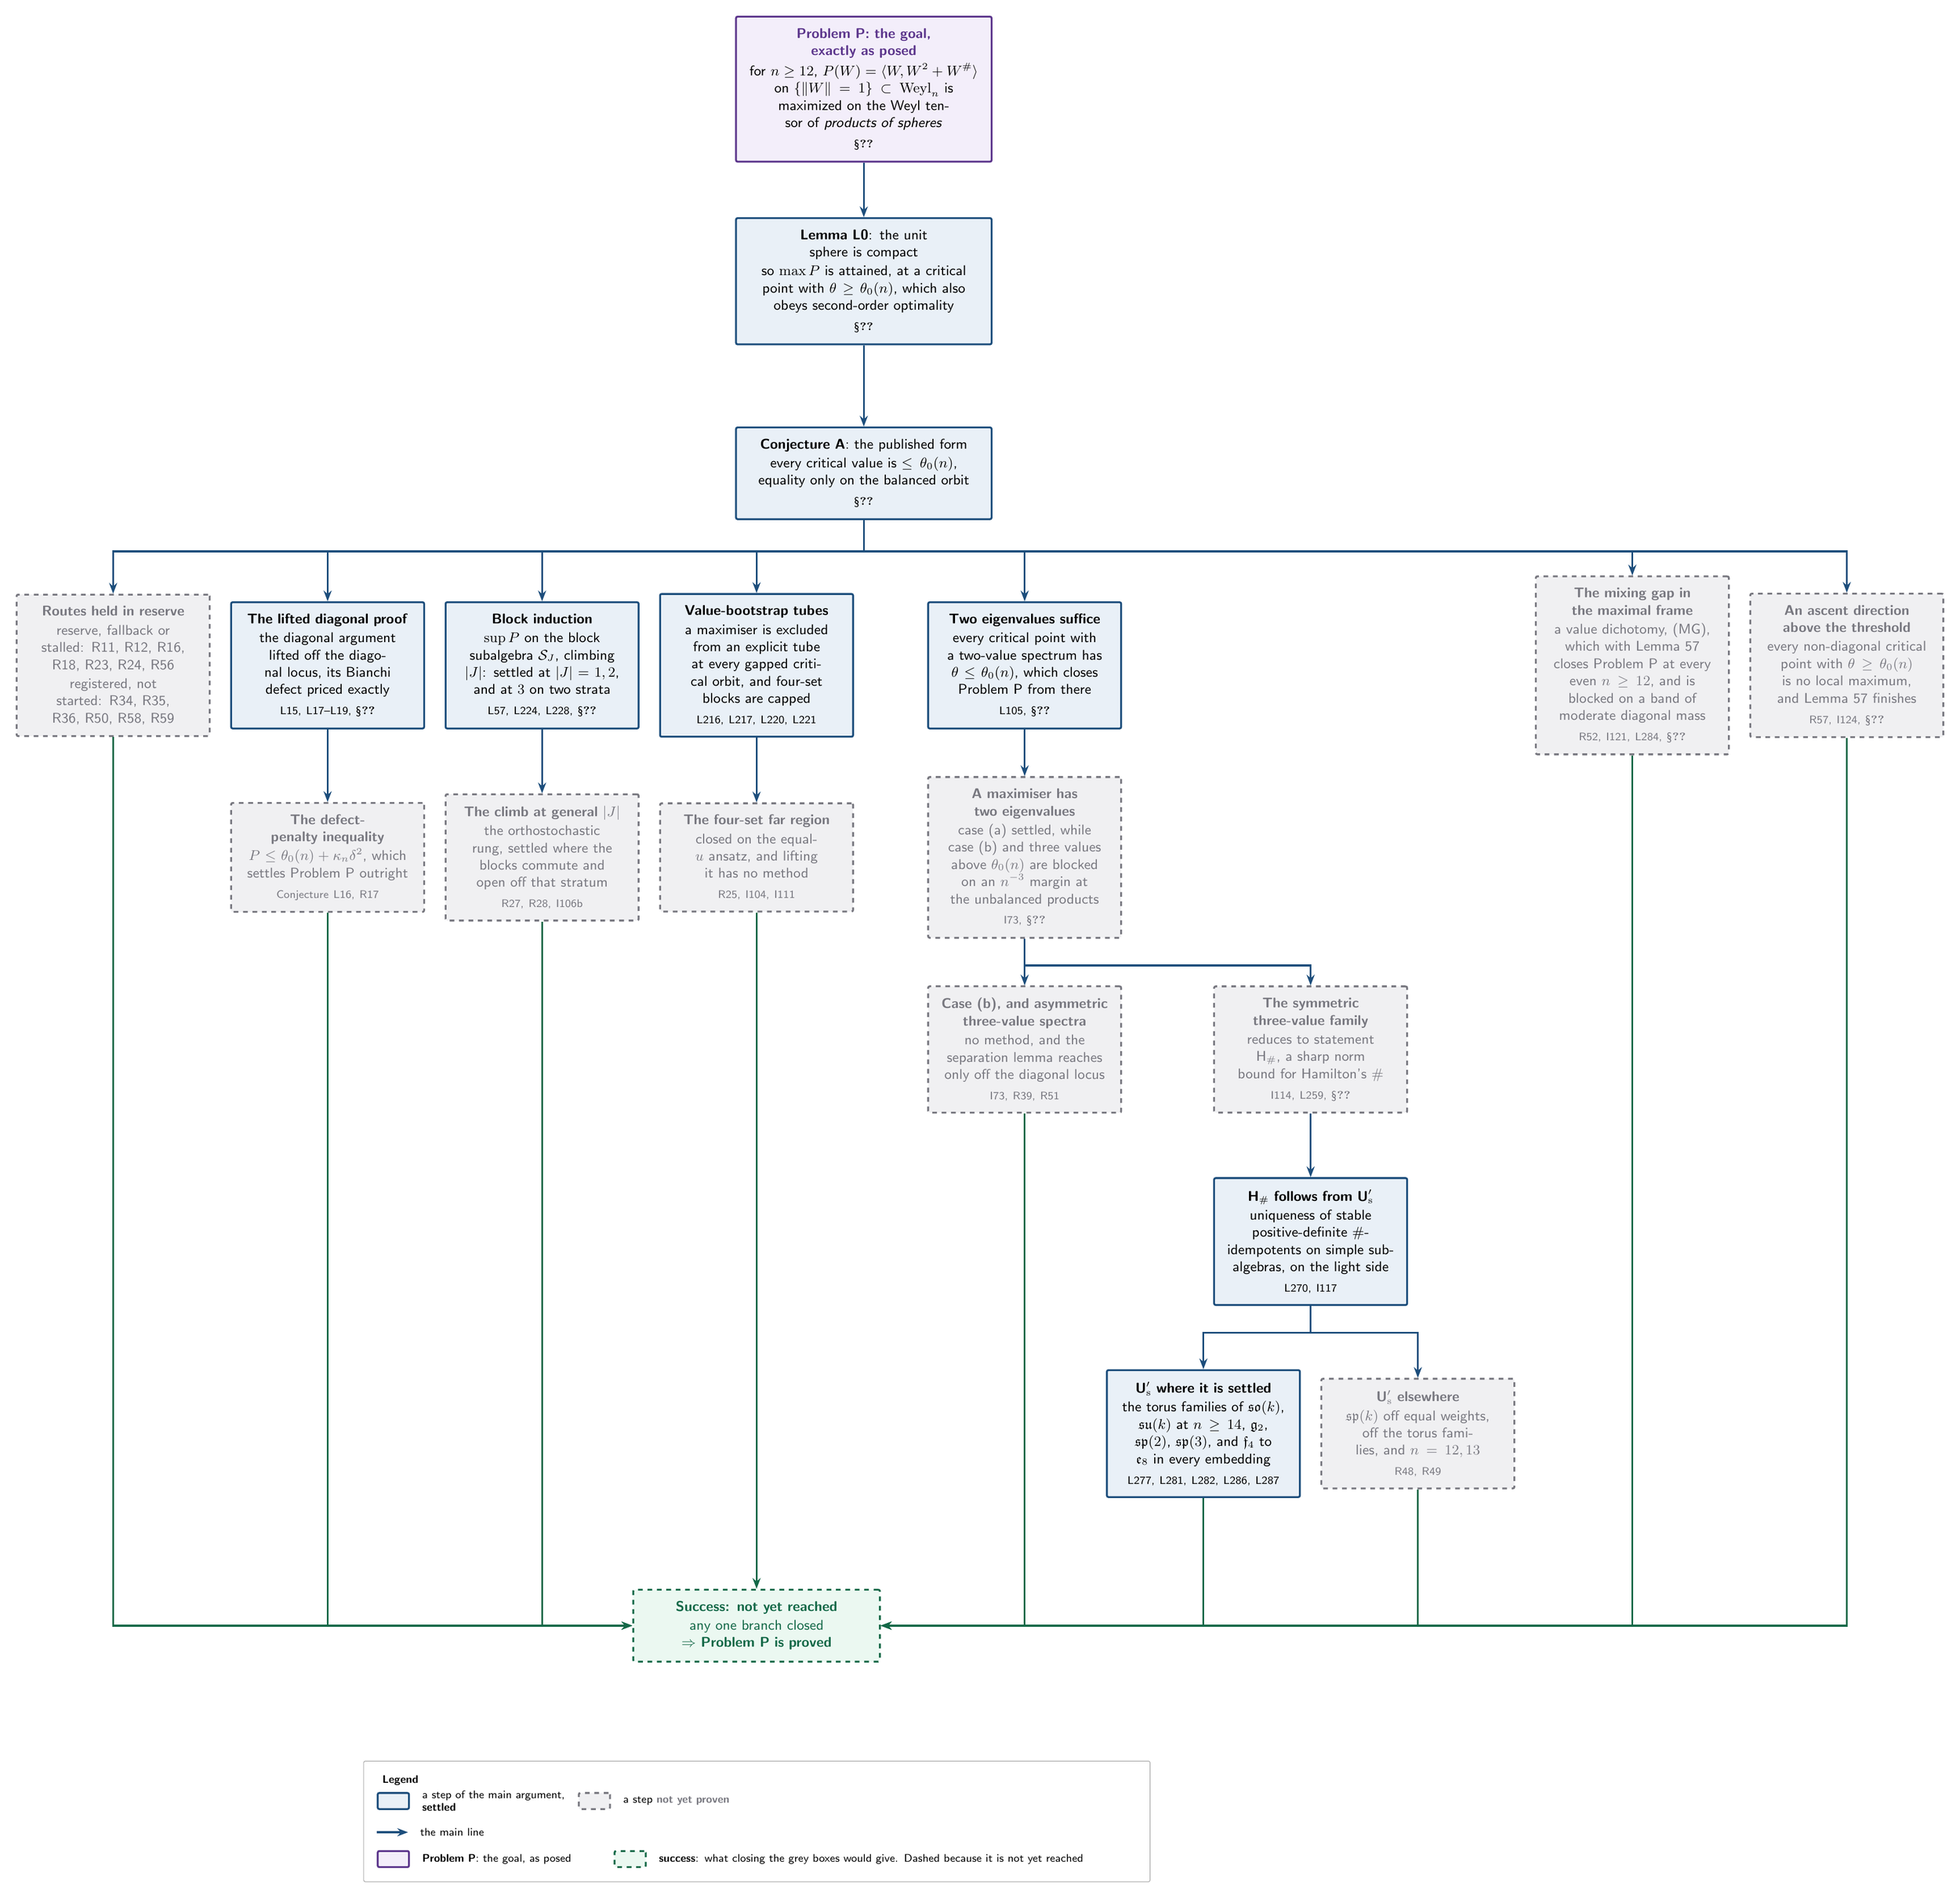
\begin{tikzpicture}[
  node distance=6mm and 9mm,
  font=\sffamily\small,
  spine/.style={draw=spineink, very thick, fill=spinebg, rounded corners=1pt,
                text width=62mm, align=center, inner sep=2.6mm},
  open/.style ={draw=openink, very thick, dashed, fill=openbg, rounded corners=1pt,
                text width=62mm, align=center, inner sep=2.6mm},
  stmt/.style ={draw=posedink, very thick, fill=posedbg, rounded corners=1pt,
                text width=76mm, align=center, inner sep=2.6mm},
  goal/.style ={draw=openink, very thick, dashed, fill=white, rounded corners=1pt,
                text width=76mm, align=center, inner sep=2.6mm},
  win/.style  ={draw=winink, very thick, dashed, fill=winbg, rounded corners=1pt,
                text width=76mm, align=center, inner sep=2.6mm},
  lem/.style  ={draw=lemink, fill=lembg, rounded corners=1pt,
                text width=40mm, align=left, inner sep=2.2mm, font=\sffamily\scriptsize},
  dead/.style ={draw=deadink, text=deadink, fill=deadbg, rounded corners=1pt,
                text width=40mm, align=left, inner sep=2.2mm, font=\sffamily\scriptsize},
  main/.style ={-{Stealth[length=2.4mm]}, spineink, very thick},
  feed/.style ={-{Stealth[length=2mm]}, lemink, dashed, thick},
  kill/.style ={-{Stealth[length=2mm]}, deadink, dashed, thick},
]

% ===================== the live routes (Figure 1, copied verbatim into Figure 3) =====================
% One branch per live strategy under Conjecture A; routes that serve a single step
% fold into that step's box, and routes held in reserve share the grey box at left.
% Rows sit at the longest-path depth from Problem P, PITCH 43mm.
\node[stmt, text width=52mm] (asked) at (0mm,0mm)
      {\textbf{\color{posedink}Problem P: the goal, exactly as posed}\\[2pt]
       for $n\ge12$, $P(W)=\langle W,W^2+W^{\#}\rangle$ on $\{\|W\|=1\}\subset\Weyl_n$ is maximized on the Weyl tensor of \emph{products of spheres}\\[2pt] {\scriptsize\S\ref{sec:problem}}};
\node[spine, text width=52mm] (compact) at (0mm,-43mm)
      {\textbf{Lemma L0}: the unit sphere is compact\\[1pt] so $\max P$ is attained, at a critical point with $\theta\ge\theta_0(n)$, which also obeys second-order optimality\\[2pt] {\scriptsize\S\ref{sec:twoforms}}};
\node[spine, text width=52mm] (restate) at (0mm,-86mm)
      {\textbf{Conjecture A}: the published form\\[1pt] every critical value is $\le\theta_0(n)$, equality only on the balanced orbit\\[2pt] {\scriptsize\S\ref{sec:twoforms}}};

\node[open, text width=38mm] (reserve) at (-168mm,-129mm)
  {\textbf{\color{openink}Routes held in reserve}\\[1pt] \color{openink}reserve, fallback or stalled: R11, R12, R16, R18, R23, R24, R56\\[1pt] registered, not started: R34, R35, R36, R50, R58, R59};
\node[spine, text width=38mm] (lift) at (-120mm,-129mm)
  {\textbf{The lifted diagonal proof}\\[1pt] the diagonal argument lifted off the diagonal locus, its Bianchi defect priced exactly\\[2pt] {\scriptsize L15, L17--L19, \S\ref{app:C}}};
\node[spine, text width=38mm] (block) at (-72mm,-129mm)
  {\textbf{Block induction}\\[1pt] $\sup P$ on the block subalgebra $\mathcal S_J$, climbing $\lvert J\rvert$: settled at $\lvert J\rvert=1,2$, and at $3$ on two strata\\[2pt] {\scriptsize L57, L224, L228, \S\ref{sec:blockinduction}}};
\node[spine, text width=38mm] (tubes) at (-24mm,-129mm)
  {\textbf{Value-bootstrap tubes}\\[1pt] a maximiser is excluded from an explicit tube at every gapped critical orbit, and four-set blocks are capped\\[2pt] {\scriptsize L216, L217, L220, L221}};
\node[spine, text width=38mm] (twoval) at (36mm,-129mm)
  {\textbf{Two eigenvalues suffice}\\[1pt] every critical point with a two-value spectrum has $\theta\le\theta_0(n)$, which closes Problem~P from there\\[2pt] {\scriptsize L105, \S\ref{sec:classsystem}}};

\node[open, text width=38mm] (l16) at (-120mm,-172mm)
  {\textbf{\color{openink}The defect-penalty inequality}\\[1pt] \color{openink}$P\le\theta_0(n)+\kappa_n\delta^2$, which settles Problem~P outright\\[2pt] {\scriptsize Conjecture L16, R17}};
\node[open, text width=38mm] (climb) at (-72mm,-172mm)
  {\textbf{\color{openink}The climb at general $\lvert J\rvert$}\\[1pt] \color{openink}the orthostochastic rung, settled where the blocks commute and open off that stratum\\[2pt] {\scriptsize R27, R28, I106b}};
\node[open, text width=38mm] (far) at (-24mm,-172mm)
  {\textbf{\color{openink}The four-set far region}\\[1pt] \color{openink}closed on the equal-$u$ ansatz, and lifting it has no method\\[2pt] {\scriptsize R25, I104, I111}};
\node[open, text width=38mm] (i73) at (36mm,-172mm)
  {\textbf{\color{openink}A maximiser has two eigenvalues}\\[1pt] \color{openink}case (a) settled, while case (b) and three values above $\theta_0(n)$ are blocked on an $n^{-3}$ margin at the unbalanced products\\[2pt] {\scriptsize I73, \S\ref{sec:classsystem}}};

\node[open, text width=38mm] (asym) at (36mm,-215mm)
  {\textbf{\color{openink}Case (b), and asymmetric three-value spectra}\\[1pt] \color{openink}no method, and the separation lemma reaches only off the diagonal locus\\[2pt] {\scriptsize I73, R39, R51}};
\node[open, text width=38mm] (sym) at (100mm,-215mm)
  {\textbf{\color{openink}The symmetric three-value family}\\[1pt] \color{openink}reduces to statement H$_\#$, a sharp norm bound for Hamilton's $\#$\\[2pt] {\scriptsize I114, L259, \S\ref{sec:statementH}}};

\node[spine, text width=38mm] (hfromu) at (100mm,-258mm)
  {\textbf{H$_\#$ follows from U$_{\mathrm s}'$}\\[1pt] uniqueness of stable positive-definite $\#$-idempotents on simple subalgebras, on the light side\\[2pt] {\scriptsize L270, I117}};

\node[spine, text width=38mm] (torus) at (76mm,-301mm)
  {\textbf{U$_{\mathrm s}'$ where it is settled}\\[1pt] the torus families of $\mathfrak{so}(k)$, $\mathfrak{su}(k)$ at $n\ge14$, $\mathfrak g_2$, $\mathfrak{sp}(2)$, $\mathfrak{sp}(3)$, and $\mathfrak f_4$ to $\mathfrak e_8$ in every embedding\\[2pt] {\scriptsize L277, L281, L282, L286, L287}};
\node[open, text width=38mm] (offtorus) at (124mm,-301mm)
  {\textbf{\color{openink}U$_{\mathrm s}'$ elsewhere}\\[1pt] \color{openink}$\mathfrak{sp}(k)$ off equal weights, off the torus families, and $n=12,13$\\[2pt] {\scriptsize R48, R49}};

\node[open, text width=38mm] (mixgap) at (172mm,-129mm)
  {\textbf{\color{openink}The mixing gap in the maximal frame}\\[1pt] \color{openink}a value dichotomy, (MG), which with Lemma~57 closes Problem~P at every even $n\ge12$, and is blocked on a band of moderate diagonal mass\\[2pt] {\scriptsize R52, I121, L284, \S\ref{sec:mixinggap}}};

\node[open, text width=38mm] (ascent) at (220mm,-129mm)
  {\textbf{\color{openink}An ascent direction above the threshold}\\[1pt] \color{openink}every non-diagonal critical point with $\theta\ge\theta_0(n)$ is no local maximum, and Lemma~57 finishes\\[2pt] {\scriptsize R57, I124, \S\ref{sec:close}}};

\node[win, text width=50mm] (win) at (-24mm,-344mm)
  {\textbf{\color{winink}Success: not yet reached}\\[1pt] \color{winink}any one branch closed $\Rightarrow$ \textbf{Problem~P is proved}};

\draw[main] (asked) -- (compact);
\draw[main] (compact) -- (restate);
\draw[main] (restate.south) -- ++(0,-7mm) -| (reserve.north);
\draw[main] (restate.south) -- ++(0,-7mm) -| (lift.north);
\draw[main] (restate.south) -- ++(0,-7mm) -| (block.north);
\draw[main] (restate.south) -- ++(0,-7mm) -| (tubes.north);
\draw[main] (restate.south) -- ++(0,-7mm) -| (twoval.north);
\draw[main] (restate.south) -- ++(0,-7mm) -| (mixgap.north);
\draw[main] (restate.south) -- ++(0,-7mm) -| (ascent.north);
\draw[main] (lift) -- (l16);
\draw[main] (block) -- (climb);
\draw[main] (tubes) -- (far);
\draw[main] (twoval) -- (i73);
\draw[main] (i73) -- (asym);
\draw[main] (i73.south) -- ++(0,-6mm) -| (sym.north);
\draw[main] (sym) -- (hfromu);
\draw[main] (hfromu.south) -- ++(0,-6mm) -| (torus.north);
\draw[main] (hfromu.south) -- ++(0,-6mm) -| (offtorus.north);
\draw[main, winink] (reserve.south) |- (win.west);
\draw[main, winink] (l16.south) |- (win.west);
\draw[main, winink] (climb.south) |- (win.west);
\draw[main, winink] (far) -- (win);
\draw[main, winink] (asym.south) |- (win.east);
\draw[main, winink] (torus.south) |- (win.east);
\draw[main, winink] (offtorus.south) |- (win.east);
\draw[main, winink] (mixgap.south) |- (win.east);
\draw[main, winink] (ascent.south) |- (win.east);

% ---------------- legend
\begin{scope}[shift={($(win.south)+(-88mm,-22mm)$)}, font=\sffamily\scriptsize]
  \node[draw=black!35, fill=white, rounded corners=1pt, inner sep=3mm,
        minimum width=176mm, minimum height=27mm, anchor=north west] (leg) at (0,0) {};
  \node[anchor=north west, font=\sffamily\scriptsize\bfseries] at ($(leg.north west)+(3mm,-2mm)$) {Legend};

  \node[draw=spineink, very thick, fill=spinebg, rounded corners=1pt,
        minimum width=7mm, minimum height=3.6mm, anchor=west] (k1) at ($(leg.north west)+(3mm,-9mm)$) {};
  \node[anchor=west, text width=34mm] at ($(k1.east)+(1.5mm,0)$) {a step of the main argument, \textbf{settled}};

  \node[draw=openink, very thick, dashed, fill=openbg, rounded corners=1pt,
        minimum width=7mm, minimum height=3.6mm, anchor=west] (k2) at ($(leg.north west)+(48mm,-9mm)$) {};
  \node[anchor=west, text width=34mm] at ($(k2.east)+(1.5mm,0)$) {a step \textbf{\color{openink}not yet proven}};


  \node[draw=posedink, very thick, fill=posedbg, rounded corners=1pt,
        minimum width=7mm, minimum height=3.6mm, anchor=west] (k5) at ($(leg.north west)+(3mm,-22mm)$) {};
  \node[anchor=west, text width=42mm] at ($(k5.east)+(1.5mm,0)$) {\textbf{Problem P}: the goal, as posed};

  \node[draw=winink, very thick, dashed, fill=winbg, rounded corners=1pt,
        minimum width=7mm, minimum height=3.6mm, anchor=west] (k6) at ($(leg.north west)+(56mm,-22mm)$) {};
  \node[anchor=west, text width=110mm] at ($(k6.east)+(1.5mm,0)$) {\textbf{success}: what closing the grey boxes would give. Dashed because it is not yet reached};



  \draw[main] ($(leg.north west)+(3mm,-16mm)$) -- ++(7mm,0);
  \node[anchor=west, text width=34mm] at ($(leg.north west)+(11.5mm,-16mm)$) {the main line};


\end{scope}

\end{tikzpicture}%
\end{adjustbox}
\caption{\textbf{The live routes towards a proof, and where each one stands.} Each branch below Conjecture~A is one live strategy, read downward as a reduction, blue settled and grey not yet proven, and the grey box at the left names the routes held in reserve. \textbf{Figure~\ref{fig:closed} is this map with the failed routes added}. Figure~\ref{fig:routes-dag} reads what the results named here rest on.}
\label{fig:routes}
\end{figure}


% GENERATED by scripts/misc/result_dag_figures.py -- do not edit
\begin{figure}[H]
\centering
\begin{adjustbox}{max width=\textwidth, max totalheight=0.78\textheight}
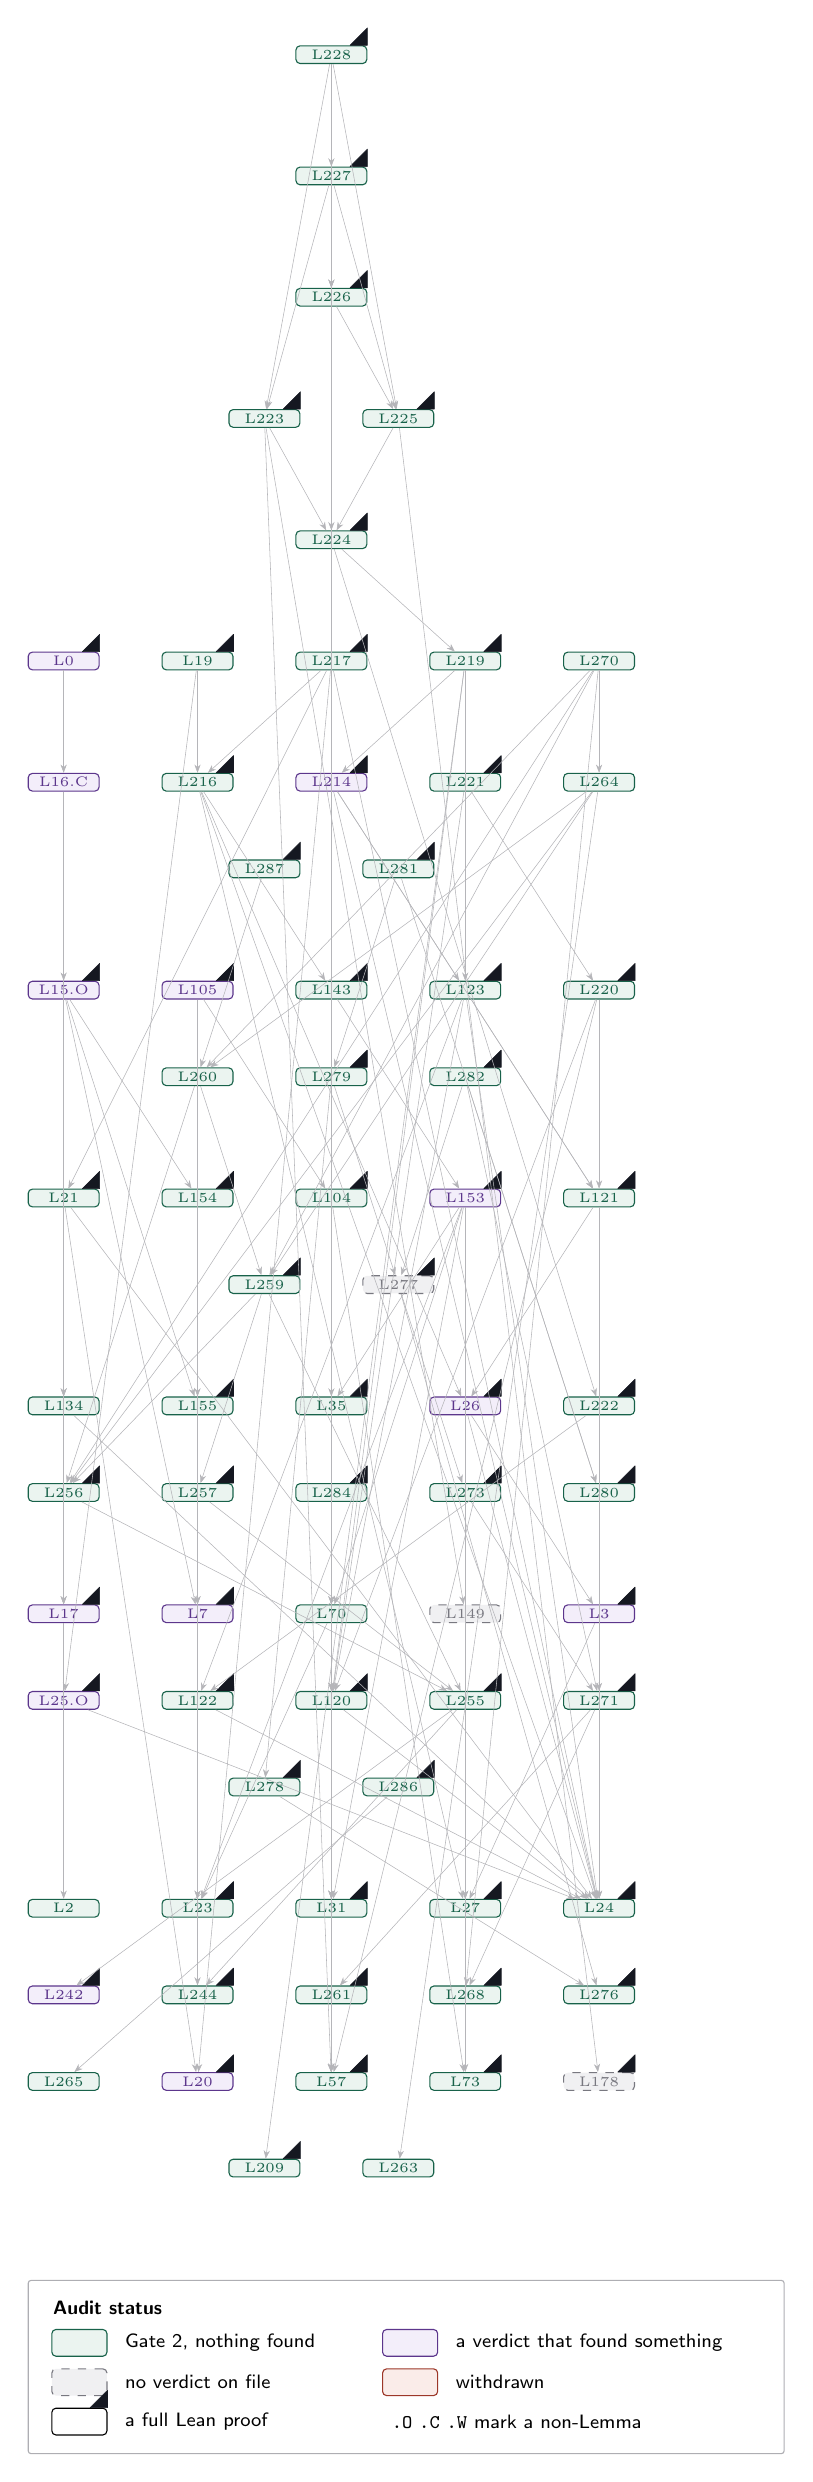
\begin{tikzpicture}[
  x=17mm,y=11mm,
  every node/.style={font=\tiny},
  res/.style={draw,rounded corners=1.5pt,inner sep=1.5pt,minimum width=9mm,align=center},
  ok/.style={res,draw=lemink,fill=lembg,text=lemink},
  gap/.style={res,draw=posedink,fill=posedbg,text=posedink},
  raw/.style={res,draw=openink,fill=openbg,text=openink,dashed},
  gone/.style={res,draw=deadink,fill=deadbg,text=deadink},
  halo/.style={res,draw=deadink,fill=deadbg,text=deadbg,inner xsep=9pt,inner ysep=7pt,minimum width=14mm,line width=.9pt},
  dep/.style={-{Stealth[length=3pt]},openink!55,line width=.2pt},
  bad/.style={-{Stealth[length=3pt]},deadink,line width=.5pt},
  lean/.style={fill=inkline,draw=inkline,line width=.2pt,line join=round},
]
\node[gap] (n0) at (-2.00,-7.00) {L0};
\node[ok] (n2) at (-2.00,-21.40) {L2};
\node[gap] (n3) at (2.00,-18.00) {L3};
\node[gap] (n7) at (-1.00,-18.00) {L7};
\node[gap] (n15) at (-2.00,-10.80) {L15.O};
\node[gap] (n16) at (-2.00,-8.40) {L16.C};
\node[gap] (n17) at (-2.00,-18.00) {L17};
\node[ok] (n19) at (-1.00,-7.00) {L19};
\node[gap] (n20) at (-1.00,-23.40) {L20};
\node[ok] (n21) at (-2.00,-13.20) {L21};
\node[ok] (n23) at (-1.00,-21.40) {L23};
\node[ok] (n24) at (2.00,-21.40) {L24};
\node[gap] (n25) at (-2.00,-19.00) {L25.O};
\node[gap] (n26) at (1.00,-15.60) {L26};
\node[ok] (n27) at (1.00,-21.40) {L27};
\node[ok] (n31) at (0.00,-21.40) {L31};
\node[ok] (n35) at (0.00,-15.60) {L35};
\node[ok] (n57) at (0.00,-23.40) {L57};
\node[ok] (n70) at (0.00,-18.00) {L70};
\node[ok] (n73) at (1.00,-23.40) {L73};
\node[ok] (n104) at (0.00,-13.20) {L104};
\node[gap] (n105) at (-1.00,-10.80) {L105};
\node[ok] (n120) at (0.00,-19.00) {L120};
\node[ok] (n121) at (2.00,-13.20) {L121};
\node[ok] (n122) at (-1.00,-19.00) {L122};
\node[ok] (n123) at (1.00,-10.80) {L123};
\node[ok] (n134) at (-2.00,-15.60) {L134};
\node[ok] (n143) at (0.00,-10.80) {L143};
\node[raw] (n149) at (1.00,-18.00) {L149};
\node[gap] (n153) at (1.00,-13.20) {L153};
\node[ok] (n154) at (-1.00,-13.20) {L154};
\node[ok] (n155) at (-1.00,-15.60) {L155};
\node[raw] (n178) at (2.00,-23.40) {L178};
\node[ok] (n209) at (-0.50,-24.40) {L209};
\node[gap] (n214) at (0.00,-8.40) {L214};
\node[ok] (n216) at (-1.00,-8.40) {L216};
\node[ok] (n217) at (0.00,-7.00) {L217};
\node[ok] (n219) at (1.00,-7.00) {L219};
\node[ok] (n220) at (2.00,-10.80) {L220};
\node[ok] (n221) at (1.00,-8.40) {L221};
\node[ok] (n222) at (2.00,-15.60) {L222};
\node[ok] (n223) at (-0.50,-4.20) {L223};
\node[ok] (n224) at (0.00,-5.60) {L224};
\node[ok] (n225) at (0.50,-4.20) {L225};
\node[ok] (n226) at (0.00,-2.80) {L226};
\node[ok] (n227) at (0.00,-1.40) {L227};
\node[ok] (n228) at (0.00,0.00) {L228};
\node[gap] (n242) at (-2.00,-22.40) {L242};
\node[ok] (n244) at (-1.00,-22.40) {L244};
\node[ok] (n255) at (1.00,-19.00) {L255};
\node[ok] (n256) at (-2.00,-16.60) {L256};
\node[ok] (n257) at (-1.00,-16.60) {L257};
\node[ok] (n259) at (-0.50,-14.20) {L259};
\node[ok] (n260) at (-1.00,-11.80) {L260};
\node[ok] (n261) at (0.00,-22.40) {L261};
\node[ok] (n263) at (0.50,-24.40) {L263};
\node[ok] (n264) at (2.00,-8.40) {L264};
\node[ok] (n265) at (-2.00,-23.40) {L265};
\node[ok] (n268) at (1.00,-22.40) {L268};
\node[ok] (n270) at (2.00,-7.00) {L270};
\node[ok] (n271) at (2.00,-19.00) {L271};
\node[ok] (n273) at (1.00,-16.60) {L273};
\node[ok] (n276) at (2.00,-22.40) {L276};
\node[raw] (n277) at (0.50,-14.20) {L277};
\node[ok] (n278) at (-0.50,-20.00) {L278};
\node[ok] (n279) at (0.00,-11.80) {L279};
\node[ok] (n280) at (2.00,-16.60) {L280};
\node[ok] (n281) at (0.50,-9.40) {L281};
\node[ok] (n282) at (1.00,-11.80) {L282};
\node[ok] (n284) at (0.00,-16.60) {L284};
\node[ok] (n286) at (0.50,-20.00) {L286};
\node[ok] (n287) at (-0.50,-9.40) {L287};
\fill[lean] (n0.north east) -- ++(-2.2mm,0) -- ++(2.2mm,2.2mm) -- cycle;
\fill[lean] (n3.north east) -- ++(-2.2mm,0) -- ++(2.2mm,2.2mm) -- cycle;
\fill[lean] (n7.north east) -- ++(-2.2mm,0) -- ++(2.2mm,2.2mm) -- cycle;
\fill[lean] (n15.north east) -- ++(-2.2mm,0) -- ++(2.2mm,2.2mm) -- cycle;
\fill[lean] (n17.north east) -- ++(-2.2mm,0) -- ++(2.2mm,2.2mm) -- cycle;
\fill[lean] (n19.north east) -- ++(-2.2mm,0) -- ++(2.2mm,2.2mm) -- cycle;
\fill[lean] (n20.north east) -- ++(-2.2mm,0) -- ++(2.2mm,2.2mm) -- cycle;
\fill[lean] (n21.north east) -- ++(-2.2mm,0) -- ++(2.2mm,2.2mm) -- cycle;
\fill[lean] (n23.north east) -- ++(-2.2mm,0) -- ++(2.2mm,2.2mm) -- cycle;
\fill[lean] (n24.north east) -- ++(-2.2mm,0) -- ++(2.2mm,2.2mm) -- cycle;
\fill[lean] (n25.north east) -- ++(-2.2mm,0) -- ++(2.2mm,2.2mm) -- cycle;
\fill[lean] (n26.north east) -- ++(-2.2mm,0) -- ++(2.2mm,2.2mm) -- cycle;
\fill[lean] (n27.north east) -- ++(-2.2mm,0) -- ++(2.2mm,2.2mm) -- cycle;
\fill[lean] (n31.north east) -- ++(-2.2mm,0) -- ++(2.2mm,2.2mm) -- cycle;
\fill[lean] (n35.north east) -- ++(-2.2mm,0) -- ++(2.2mm,2.2mm) -- cycle;
\fill[lean] (n57.north east) -- ++(-2.2mm,0) -- ++(2.2mm,2.2mm) -- cycle;
\fill[lean] (n73.north east) -- ++(-2.2mm,0) -- ++(2.2mm,2.2mm) -- cycle;
\fill[lean] (n104.north east) -- ++(-2.2mm,0) -- ++(2.2mm,2.2mm) -- cycle;
\fill[lean] (n105.north east) -- ++(-2.2mm,0) -- ++(2.2mm,2.2mm) -- cycle;
\fill[lean] (n120.north east) -- ++(-2.2mm,0) -- ++(2.2mm,2.2mm) -- cycle;
\fill[lean] (n121.north east) -- ++(-2.2mm,0) -- ++(2.2mm,2.2mm) -- cycle;
\fill[lean] (n122.north east) -- ++(-2.2mm,0) -- ++(2.2mm,2.2mm) -- cycle;
\fill[lean] (n123.north east) -- ++(-2.2mm,0) -- ++(2.2mm,2.2mm) -- cycle;
\fill[lean] (n143.north east) -- ++(-2.2mm,0) -- ++(2.2mm,2.2mm) -- cycle;
\fill[lean] (n153.north east) -- ++(-2.2mm,0) -- ++(2.2mm,2.2mm) -- cycle;
\fill[lean] (n154.north east) -- ++(-2.2mm,0) -- ++(2.2mm,2.2mm) -- cycle;
\fill[lean] (n155.north east) -- ++(-2.2mm,0) -- ++(2.2mm,2.2mm) -- cycle;
\fill[lean] (n178.north east) -- ++(-2.2mm,0) -- ++(2.2mm,2.2mm) -- cycle;
\fill[lean] (n209.north east) -- ++(-2.2mm,0) -- ++(2.2mm,2.2mm) -- cycle;
\fill[lean] (n214.north east) -- ++(-2.2mm,0) -- ++(2.2mm,2.2mm) -- cycle;
\fill[lean] (n216.north east) -- ++(-2.2mm,0) -- ++(2.2mm,2.2mm) -- cycle;
\fill[lean] (n217.north east) -- ++(-2.2mm,0) -- ++(2.2mm,2.2mm) -- cycle;
\fill[lean] (n219.north east) -- ++(-2.2mm,0) -- ++(2.2mm,2.2mm) -- cycle;
\fill[lean] (n220.north east) -- ++(-2.2mm,0) -- ++(2.2mm,2.2mm) -- cycle;
\fill[lean] (n221.north east) -- ++(-2.2mm,0) -- ++(2.2mm,2.2mm) -- cycle;
\fill[lean] (n222.north east) -- ++(-2.2mm,0) -- ++(2.2mm,2.2mm) -- cycle;
\fill[lean] (n223.north east) -- ++(-2.2mm,0) -- ++(2.2mm,2.2mm) -- cycle;
\fill[lean] (n224.north east) -- ++(-2.2mm,0) -- ++(2.2mm,2.2mm) -- cycle;
\fill[lean] (n225.north east) -- ++(-2.2mm,0) -- ++(2.2mm,2.2mm) -- cycle;
\fill[lean] (n226.north east) -- ++(-2.2mm,0) -- ++(2.2mm,2.2mm) -- cycle;
\fill[lean] (n227.north east) -- ++(-2.2mm,0) -- ++(2.2mm,2.2mm) -- cycle;
\fill[lean] (n228.north east) -- ++(-2.2mm,0) -- ++(2.2mm,2.2mm) -- cycle;
\fill[lean] (n242.north east) -- ++(-2.2mm,0) -- ++(2.2mm,2.2mm) -- cycle;
\fill[lean] (n244.north east) -- ++(-2.2mm,0) -- ++(2.2mm,2.2mm) -- cycle;
\fill[lean] (n255.north east) -- ++(-2.2mm,0) -- ++(2.2mm,2.2mm) -- cycle;
\fill[lean] (n256.north east) -- ++(-2.2mm,0) -- ++(2.2mm,2.2mm) -- cycle;
\fill[lean] (n257.north east) -- ++(-2.2mm,0) -- ++(2.2mm,2.2mm) -- cycle;
\fill[lean] (n259.north east) -- ++(-2.2mm,0) -- ++(2.2mm,2.2mm) -- cycle;
\fill[lean] (n261.north east) -- ++(-2.2mm,0) -- ++(2.2mm,2.2mm) -- cycle;
\fill[lean] (n268.north east) -- ++(-2.2mm,0) -- ++(2.2mm,2.2mm) -- cycle;
\fill[lean] (n271.north east) -- ++(-2.2mm,0) -- ++(2.2mm,2.2mm) -- cycle;
\fill[lean] (n273.north east) -- ++(-2.2mm,0) -- ++(2.2mm,2.2mm) -- cycle;
\fill[lean] (n276.north east) -- ++(-2.2mm,0) -- ++(2.2mm,2.2mm) -- cycle;
\fill[lean] (n277.north east) -- ++(-2.2mm,0) -- ++(2.2mm,2.2mm) -- cycle;
\fill[lean] (n278.north east) -- ++(-2.2mm,0) -- ++(2.2mm,2.2mm) -- cycle;
\fill[lean] (n279.north east) -- ++(-2.2mm,0) -- ++(2.2mm,2.2mm) -- cycle;
\fill[lean] (n280.north east) -- ++(-2.2mm,0) -- ++(2.2mm,2.2mm) -- cycle;
\fill[lean] (n281.north east) -- ++(-2.2mm,0) -- ++(2.2mm,2.2mm) -- cycle;
\fill[lean] (n282.north east) -- ++(-2.2mm,0) -- ++(2.2mm,2.2mm) -- cycle;
\fill[lean] (n284.north east) -- ++(-2.2mm,0) -- ++(2.2mm,2.2mm) -- cycle;
\fill[lean] (n286.north east) -- ++(-2.2mm,0) -- ++(2.2mm,2.2mm) -- cycle;
\fill[lean] (n287.north east) -- ++(-2.2mm,0) -- ++(2.2mm,2.2mm) -- cycle;
\draw[dep] (n0) -- (n16);
\draw[dep] (n3) -- (n24);
\draw[dep] (n3) -- (n27);
\draw[dep] (n7) -- (n23);
\draw[dep] (n15) -- (n7);
\draw[dep] (n15) -- (n154);
\draw[dep] (n15) -- (n155);
\draw[dep] (n16) -- (n15);
\draw[dep] (n16) -- (n17);
\draw[dep] (n16) -- (n134);
\draw[dep] (n17) -- (n2);
\draw[dep] (n19) -- (n25);
\draw[dep] (n19) -- (n216);
\draw[dep] (n21) -- (n20);
\draw[dep] (n21) -- (n24);
\draw[dep] (n21) -- (n134);
\draw[dep] (n25) -- (n24);
\draw[dep] (n26) -- (n3);
\draw[dep] (n26) -- (n24);
\draw[dep] (n26) -- (n27);
\draw[dep] (n35) -- (n70);
\draw[dep] (n70) -- (n23);
\draw[dep] (n70) -- (n31);
\draw[dep] (n104) -- (n31);
\draw[dep] (n104) -- (n35);
\draw[dep] (n104) -- (n73);
\draw[dep] (n105) -- (n23);
\draw[dep] (n105) -- (n104);
\draw[dep] (n120) -- (n24);
\draw[dep] (n121) -- (n24);
\draw[dep] (n121) -- (n26);
\draw[dep] (n122) -- (n24);
\draw[dep] (n123) -- (n24);
\draw[dep] (n123) -- (n120);
\draw[dep] (n123) -- (n121);
\draw[dep] (n123) -- (n122);
\draw[dep] (n134) -- (n17);
\draw[dep] (n134) -- (n24);
\draw[dep] (n143) -- (n31);
\draw[dep] (n143) -- (n70);
\draw[dep] (n143) -- (n153);
\draw[dep] (n149) -- (n27);
\draw[dep] (n153) -- (n23);
\draw[dep] (n153) -- (n31);
\draw[dep] (n153) -- (n35);
\draw[dep] (n153) -- (n70);
\draw[dep] (n153) -- (n73);
\draw[dep] (n154) -- (n7);
\draw[dep] (n154) -- (n155);
\draw[dep] (n155) -- (n7);
\draw[dep] (n214) -- (n24);
\draw[dep] (n214) -- (n120);
\draw[dep] (n214) -- (n121);
\draw[dep] (n214) -- (n123);
\draw[dep] (n216) -- (n24);
\draw[dep] (n216) -- (n26);
\draw[dep] (n216) -- (n27);
\draw[dep] (n216) -- (n143);
\draw[dep] (n217) -- (n20);
\draw[dep] (n217) -- (n21);
\draw[dep] (n217) -- (n24);
\draw[dep] (n217) -- (n216);
\draw[dep] (n219) -- (n120);
\draw[dep] (n219) -- (n123);
\draw[dep] (n219) -- (n209);
\draw[dep] (n219) -- (n214);
\draw[dep] (n220) -- (n57);
\draw[dep] (n220) -- (n120);
\draw[dep] (n220) -- (n121);
\draw[dep] (n221) -- (n120);
\draw[dep] (n221) -- (n220);
\draw[dep] (n222) -- (n122);
\draw[dep] (n223) -- (n57);
\draw[dep] (n223) -- (n149);
\draw[dep] (n223) -- (n224);
\draw[dep] (n224) -- (n57);
\draw[dep] (n224) -- (n120);
\draw[dep] (n224) -- (n219);
\draw[dep] (n224) -- (n222);
\draw[dep] (n225) -- (n178);
\draw[dep] (n225) -- (n224);
\draw[dep] (n226) -- (n224);
\draw[dep] (n226) -- (n225);
\draw[dep] (n227) -- (n57);
\draw[dep] (n227) -- (n223);
\draw[dep] (n227) -- (n225);
\draw[dep] (n227) -- (n226);
\draw[dep] (n228) -- (n57);
\draw[dep] (n228) -- (n223);
\draw[dep] (n228) -- (n225);
\draw[dep] (n228) -- (n226);
\draw[dep] (n228) -- (n227);
\draw[dep] (n255) -- (n244);
\draw[dep] (n255) -- (n242);
\draw[dep] (n256) -- (n255);
\draw[dep] (n257) -- (n255);
\draw[dep] (n257) -- (n244);
\draw[dep] (n282) -- (n271);
\draw[dep] (n282) -- (n277);
\draw[dep] (n282) -- (n280);
\draw[dep] (n281) -- (n280);
\draw[dep] (n281) -- (n279);
\draw[dep] (n280) -- (n271);
\draw[dep] (n279) -- (n278);
\draw[dep] (n279) -- (n277);
\draw[dep] (n278) -- (n276);
\draw[dep] (n277) -- (n273);
\draw[dep] (n277) -- (n276);
\draw[dep] (n273) -- (n271);
\draw[dep] (n271) -- (n261);
\draw[dep] (n271) -- (n268);
\draw[dep] (n270) -- (n256);
\draw[dep] (n270) -- (n260);
\draw[dep] (n270) -- (n264);
\draw[dep] (n270) -- (n268);
\draw[dep] (n270) -- (n259);
\draw[dep] (n264) -- (n260);
\draw[dep] (n264) -- (n263);
\draw[dep] (n264) -- (n256);
\draw[dep] (n264) -- (n259);
\draw[dep] (n260) -- (n259);
\draw[dep] (n260) -- (n256);
\draw[dep] (n259) -- (n257);
\draw[dep] (n259) -- (n255);
\draw[dep] (n259) -- (n256);
\draw[dep] (n284) -- (n120);
\draw[dep] (n286) -- (n265);
\draw[dep] (n287) -- (n260);
% legend: the colour convention belongs in the picture, where a reader meets it
\begin{scope}[shift={($(current bounding box.south west)+(0,-13mm)$)}]
  \node[draw=openink!60,rounded corners=1pt,minimum width=96mm,minimum height=22mm,
        anchor=north west,font=\sffamily\scriptsize] (leg) at (0,0) {};
  \node[anchor=north west,font=\sffamily\scriptsize\bfseries] at ($(leg.north west)+(2mm,-1.5mm)$) {Audit status};
  \node[ok,anchor=west,minimum width=7mm,minimum height=3.4mm,inner sep=0pt] (g1) at ($(leg.north west)+(3mm,-8mm)$) {};
  \node[anchor=west,font=\sffamily\scriptsize] at ($(g1.east)+(1mm,0)$) {Gate~2, nothing found};
  \node[gap,anchor=west,minimum width=7mm,minimum height=3.4mm,inner sep=0pt] (g2) at ($(leg.north west)+(45mm,-8mm)$) {};
  \node[anchor=west,font=\sffamily\scriptsize] at ($(g2.east)+(1mm,0)$) {a verdict that found something};
  \node[raw,anchor=west,minimum width=7mm,minimum height=3.4mm,inner sep=0pt] (g3) at ($(leg.north west)+(3mm,-13mm)$) {};
  \node[anchor=west,font=\sffamily\scriptsize] at ($(g3.east)+(1mm,0)$) {no verdict on file};
  \node[gone,anchor=west,minimum width=7mm,minimum height=3.4mm,inner sep=0pt] (g4) at ($(leg.north west)+(45mm,-13mm)$) {};
  \node[anchor=west,font=\sffamily\scriptsize] at ($(g4.east)+(1mm,0)$) {withdrawn};
  \node[res,anchor=west,minimum width=7mm,minimum height=3.4mm,inner sep=0pt] (g5) at ($(leg.north west)+(3mm,-18mm)$) {};
  \fill[lean] (g5.north east) -- ++(-2.2mm,0) -- ++(2.2mm,2.2mm) -- cycle;
  \node[anchor=west,font=\sffamily\scriptsize] at ($(g5.east)+(1mm,0)$) {a full Lean proof};
  \node[anchor=west,font=\sffamily\scriptsize] at ($(leg.north west)+(45mm,-18mm)$) {\texttt{.O} \texttt{.C} \texttt{.W} mark a non-Lemma};
\end{scope}
\end{tikzpicture}
\end{adjustbox}
\caption{\textbf{What the results of Figure~\ref{fig:routes} rest on.} Each arrow runs from a result to one it depends on, read off the record's own citations. \textbf{Figure~\ref{fig:closed-dag} is this reading for the closed routes}, and Figure~\ref{fig:full-dag} carries every numbered result.}
\label{fig:routes-dag}
\end{figure}


Figure~\ref{fig:closed}, in \S\ref{sec:closedroutes}, maps the \emph{failed} routes onto the same line, one red branch per route, positioned at the step it was aimed at.

\subsection{Where the work stands}

Nine facts fix the shape of the problem. \textbf{The full ledger (every result, with the qualification each carries) is \S\ref{sec:ledger}}. This table is the orientation, not the record.

\begin{center}
\begin{tabular}{@{}p{0.46\linewidth}p{0.48\linewidth}@{}}
\toprule
\textbf{Component} & \textbf{State} \\
\midrule
The diagonal case & \textbf{Proved at every $n\ge4$}, both parities, with its equality case (Lemma~57), so the grant carries nothing the report needs \\
The dimension threshold $n\ge12$ & Derived exactly as $n=6+2\sqrt7$ (Lemma~2), and \textbf{necessary}: $\Omega_0$ is non-invariant for $4\le n\le11$ (Lemma~44) \\
The target constant $\theta_0(n)$ & \textbf{Demanded by cone invariance} at $a=0$, independently of the sphere products (Lemma~43) \\
Conjecture~A on the compact symmetric spaces & \textbf{Proved} for every $n\ge12$, equality exactly at $S^{n/2}\times S^{n/2}$ (Lemmas~47, 48) \\
$P$ as a function of two spectra & \textbf{Proved}: $\theta=\tfrac32p_3(\mu)-\tfrac12p_3(\omega)$ (Lemma~50). The collapse to one spectrum is Lovelock's identity and reaches only $n\le5$ (Lemma~51) \\
A transfer inequality between the two cubics & \textbf{Open}, and it is what the bi-spectral route needs \\
The residual, as a value bound & \textbf{Open}: one inequality, and it closes every even $n\ge12$ (\S\ref{sec:outside}) \\
Maximizers away from the $\CP^2$ orbit & \textbf{Open}: this is the core problem \\
Odd $n$ & Open exactly where even $n$ is open: the non-diagonal half \\
\bottomrule
\end{tabular}
\end{center}{Provenance}

No single paper states the result end to end. It is B\"ohm--Wilking's ``Conjecture A'' (``Conjecture L1'' in some of the surrounding literature), sitting inside the curvature-operator programme of \cite{bw2008}, and it is referenced by name in Nienhaus's thesis work \cite{nienhaus2023}, whose Conjecture~A is the critical-point form of Problem~P. The identification, and why the two are the same statement, is \S\ref{sec:twoforms}. Partial progress in a related direction appears in \cite{xu2024}. The algebraic object $P$, the cubic form attached to the polarization of $Q$, is treated in generality by Fox \cite{fox2019}, who shows that the Weyl operators form a simple commutative nonassociative algebra whose idempotents are exactly the critical points of $P$ on the unit sphere.

\subsection{Labels, and how results are graded}\label{sec:labels}

Labels in this report are literal and are used consistently:
\begin{itemize}[nosep,leftmargin=1.4em]
\item \textbf{Lemma}: proven. Where a proof rests on a machine computation, the computation is exact (rational, integer, modular, or validated interval arithmetic) and this is stated.
\item \textbf{Observation}: verified numerically at the dimensions named, not proven.
\item \textbf{Conjecture}: a candidate statement, not proven, with the evidence for it stated.
\item \textbf{False}: a statement that does not hold, carried with the witness that settles it. These are kept because a negative is a result: it fences a route, and one that is not written down is paid for a second time. Where only a stronger reading fails, the row says which reading and the narrow form stays.
\end{itemize}

A fourth convention governs the proofs themselves. A \emph{proof} is an argument. A \emph{Verification} block is a machine computation, and it names the arithmetic it was done in, because the distinction decides what the result can carry: modular arithmetic bounds a kernel from above and so settles nondegeneracy but never degeneracy, and floating point settles neither. Every lemma below carries a proof. Where a proof leans on a step that is verified rather than argued (four coupling vanishings in Lemma~22, the cross-term grant in Lemma~18), that step is named at the point of use and never absorbed into the surrounding prose.

Every load-bearing result is rebuilt from definitions by two independent reviewers, each given the claim and not the code, working the same brief. Agreement between two implementations is the evidence a \textbf{Proven} label rests on, and disagreement between them is a result of its own, since exactly one side is then wrong. A result whose audit is owed says so at the point of use, and the debt ledger of \S\ref{sec:debt} collects them. \textbf{Nothing on that ledger is cited elsewhere as settled}. A result marked \emph{machine-checked in Lean} has its statement typed and its proof checked by the Lean kernel, resting on Lean's three standard axioms and on no \texttt{sorry}. That is a third line of evidence beside the two audits: the kernel checks every step of the argument it is given, and the one thing it cannot check, that the typed statement is the lemma as stated here, is compared by hand.


% ==============================================================================

\section{The question as it was asked, in plain terms}\label{sec:plain}

\emph{A notational warning that applies throughout: a reference of the form \S3.3 or \S3.5 always means a section of J\"ager's thesis, never of this report, whose own sections are referenced by a single number.}

\emph{This section assumes no differential geometry. It records the question exactly as it reached us, says what the objects in it are, and shows how the informal sentence becomes the formal statement of \S1. A reader who wants only that can stop at the end of this section.}

\subsection{The message}

The problem arrived as a chat message on 19 August 2026. Its mathematical content, quoted exactly as sent:

\begin{quote}
\small
\texttt{Consider the space W\_n of algebraic Weyl curvature operators in R\textasciicircum n. Let Q(W) = W\textasciicircum 2+W\textasciicircum\# be the quadratic map of Hamilton, sending W\_n to itself. Prove that the cubic P(W) = \textless W, Q(W)\textgreater{} (when restricted to W of norm 1) is maximized on the Weyl tensor of products of spheres when n \textbackslash geq 12. You may assume that this result is known when P is restricted to curvature operators that are diagonal with respect to a suitable basis of R\textasciicircum n.}
\end{quote}

\subsection{What the objects are}

\paragraph{Curvature, as an operator.} On a curved space, the curvature at a point is not a single number. It records how much the space bends in each two-dimensional direction: each little plane through the point. Packaging that data as a linear operator acting on the space of such planes gives the \emph{curvature operator}. In $n$ dimensions there are $\binom n2$ independent planes, so this is an operator on a space of that size.

\paragraph{The Weyl part.} A curvature operator splits into two pieces: an averaged part, which records how volumes are distorted, and the remainder, which records the pure change of shape. The remainder is the \emph{Weyl} part, and $\Weyl_n$ is the space of all algebraically possible ones in dimension $n$. Restricting attention to it removes the part of the curvature that any simple scaling argument would already control.

\paragraph{Hamilton's map $Q$, and why anyone cares.} $Q(W)=W^2+W^{\#}$ is the nonlinear term in Hamilton's Ricci flow (the equation that smooths a geometry out over time, and the tool Perelman used on the Poincar\'e conjecture). Under that flow the curvature operator evolves as
\[
\frac{\partial R}{\partial t}=\Delta R+Q(R),
\]
so $Q$ is precisely the reaction term: the part that decides which curvature conditions survive the flow and which are destroyed by it. Questions about $Q$ are therefore questions about what the flow preserves, which is what makes an inequality about it worth having.

\paragraph{The cubic $P$, and the unit sphere.} $P(W)=\langle W,Q(W)\rangle$ measures how much of $Q(W)$ points back along $W$ itself: how efficiently a given curvature shape reinforces itself under the flow. It is \emph{cubic}: replacing $W$ by $tW$ multiplies $P$ by $t^3$. So asking for a maximum only makes sense after fixing the size, which is what ``restricted to $W$ of norm~1'' does. The question is then about shape alone: among all curvature shapes of a fixed size, which one is most efficient?

\paragraph{The answer that is conjectured.} Take two round spheres of the same dimension and multiply them together: $S^{n/2}\times S^{n/2}$, a space that is round in two independent halves of its directions. The conjecture says its curvature shape is the winner, and that nothing else ties it, once $n\ge12$.

\paragraph{Why 12, of all numbers.} Because below that a different shape wins. Built from the complex projective plane $\CP^2$, it is a curvature shape whose efficiency is $\sqrt{3/2}\approx1.2247$ in \emph{every} dimension. It does not improve as space gets roomier. The sphere product's efficiency does improve with $n$, and it overtakes the rival at
\[
n=6+2\sqrt7\approx11.2915 .
\]
Twelve is simply the first whole number past that. This is not a threshold chosen to make a proof work: it is derived, three independent ways, in Lemma~2, and below it the conjecture is genuinely false.

\subsection{From the sentence to the statement}

Each phrase of the message corresponds to one formal object. The formal statement itself is Conjecture~A in \S\ref{sec:formal}.

\begin{center}
\begin{tabular}{@{}p{0.42\linewidth}p{0.54\linewidth}@{}}
\toprule
\textbf{As it was written} & \textbf{What it means formally} \\
\midrule
``the space $W_n$ of algebraic Weyl curvature operators'' & $\Weyl_n$: self-adjoint operators on $\Lambda^2\R^n$ obeying the first Bianchi identity with vanishing Ricci contraction \\
``$Q(W)=W^2+W^{\#}$, the quadratic map of Hamilton'' & The reaction term of Ricci flow, where $\#$ is the Lie-algebra square built from the structure constants of $\so(n)$ \\
``the cubic $P(W)=\langle W,Q(W)\rangle$'' & The cubic form whose critical points on the unit sphere are exactly the idempotents of Fox's nonassociative algebra \\
``restricted to $W$ of norm 1'' & Restriction to $\Weyl^1_n$, which is compact, so a maximizer exists, and is a critical point \\
``maximized on the Weyl tensor of products of spheres'' & The maximum is attained on the $SO(n)$-orbit of $W^{*}$, the Weyl operator of $S^{n/2}\times S^{n/2}$, of value $\theta_0(n)=\sqrt{2(n-1)(n-2)}/n$ \\
``when $n\ge12$'' & The threshold $n>6+2\sqrt7$, below which the $\CP^2$-type rival wins \\
``you may assume \dots\ diagonal with respect to a suitable basis'' & The case where $W$ is diagonal in the coordinate $2$-planes $e_i\wedge e_j$ of an orthonormal frame \\
\bottomrule
\end{tabular}
\end{center}

Two things are worth drawing out of that table, because they shape everything afterwards.

\paragraph{``Maximized on'' is a statement about a whole orbit, not a point.} Rotating a curvature shape does not change how efficient it is, so if $W^{*}$ is a maximizer then so is every rotation of it. The conjecture asserts that these rotations are the \emph{only} maximizers, which is why the report keeps track of orbits and of ``rigidity'' (whether anything else can sit next to one).

\paragraph{The granted assumption is a strong one, and it is where the difficulty hides.} ``Diagonal with respect to a suitable basis'' means the curvature does not mix the chosen directions: in a well-chosen coordinate frame, each little plane $e_i\wedge e_j$ is stretched by its own factor and nothing leaks between planes. That is the analogue of a diagonal matrix versus a general one. The natural hope is that the general case reduces to it by choosing the right frame, but \S\ref{sec:landscape} shows it does not: the actual rival maximizer is \emph{provably} not diagonalizable in any orthonormal frame, by three independent arguments.

\subsection{What turned out to be true about the granted assumption}

The last sentence of the message grants the diagonal case as known. Establishing what that grant actually buys meant finding the source, and the source is Florian J\"ager's 2016 M\"unster thesis \cite{jaeger2016}, locating which changed the shape of the problem. Its main theorem proves the diagonal case for even $n\ge16$, but the sentence immediately following it says the case $n\ge12$ is conjectural. So the assumption the problem statement grants was, in the literature, \textbf{unavailable at exactly the dimensions the conjecture turns on}, $n=12$ and $n=14$, and unavailable for odd $n$ at all.

Lemma~1 closes $n=12$ and $n=14$, from scratch. That is why \S\ref{sec:granted} comes before anything else: the foundation the rest of the work stands on had to be repaired before it could be stood on.

\subsection{How far it has got, without symbols}

\begin{itemize}[leftmargin=1.4em]
\item \textbf{The conjecture is not proved.} It remains open, as the sender predicted it would be.
\item \textbf{The foundation is repaired.} The granted assumption now genuinely holds at the dimensions where the question bites.
\item \textbf{The threshold is explained.} $n\ge12$ is derived rather than assumed, and the rival that beats the sphere product below it is identified exactly.
\item \textbf{No rival survives.} Every named candidate, including several catalogued here, is eliminated by computing its efficiency and finding it short.
\item \textbf{The conjectured winner is rigid, and so is every one of its rivals with symmetry.} Nothing else can sit next to a sphere product: it is an isolated peak, now proved rather than measured, for every way of splitting it into two factors apart from one small exception (Lemmas~26, 27). The same holds, with no exception at all, for the other symmetric family (Lemma~28). That rigidity is what makes the main line of attack work at all.
\item \textbf{The main argument has a working mechanism, and what is left is one inequality.} Because every symmetric shape is an isolated peak, the symmetric shapes form separate ``islands'' in the landscape of stationary shapes. What remains is to show that nothing off those islands climbs as high as the rival: a single bound, which would settle the whole conjecture for every even dimension from twelve upward, since the other half of the question is exactly what the problem statement hands you (\S\ref{sec:outside}).
\item \textbf{One region of the search space is closed unconditionally.} No maximizer can lie anywhere near the rival's shape, in any dimension from 12 upward (Lemma~20). This is a genuine theorem about the whole problem, not about a special case.
\item \textbf{One infinite family is settled completely.} On curvature shapes built from a subalgebra of rotations, the conjecture is \emph{proved outright}, with its equality case, in every dimension (Lemma~23). The proof is short: three identities and one observation that a sum of squares cannot be negative.
\item \textbf{The problem has a shape rather than a list.} It splits into three statements (\S\ref{sec:shape}). Two are settled: the sphere products really are ordered the way they must be, and among the shapes with the right kind of symmetry the balanced product wins. The third (that a genuine maximizer must have that symmetry in the first place) is open, and is the whole difficulty.
\item \textbf{The unknown maximizer is pinned from two sides.} Every earlier argument used only the condition that says a maximizer is a stationary point. A maximizer also has to \emph{curve downward} in every direction, and that turns out to be a clean eigenvalue bound (Lemma~24). Every curvature shape on record lacking the required symmetry fails it (Observation~25).
\item \textbf{The one inequality that remains is a well-defined question.} It quantifies over the curvature shapes that cannot be written in a ``diagonal'' form, and there is a test for that which does not depend on the coordinates you pick (Lemma~37), which matters, because a test that did would leave the set being quantified over undefined. Under it the bound is not merely satisfied but \emph{attained}, at the rival shape itself, in three independent searches.
\item \textbf{It is the diagonal condition doing the work, not the symmetry condition.} Among the shapes with zero slack there are ones climbing much higher than the rival: the sphere products themselves. What keeps them out of the remaining question is that they \emph{are} diagonal. Any proof has to carry that condition all the way through. One that uses only the slack is bounding a much larger set.
\item \textbf{Every curvature shape coming from a symmetric space is settled, at every dimension from twelve upward.} That is the whole of Cartan's classification (the complex and quaternionic projective spaces, the Grassmannians, the compact Lie groups, the exceptional spaces, and every product of them), and on all of it the balanced sphere product wins, uniquely (\S\ref{sec:symmetric}). The argument is a counting one: a symmetric space whose symmetry group is small cannot be efficient, and the only spaces with a large enough symmetry group are the sphere products themselves. It is worth saying what this does \emph{not} settle: having zero slack is a weaker condition than coming from a symmetric space, and the shapes in between are still owed.
\item \textbf{The target number and the dimension twelve are both forced from outside the sphere products.} The efficiency $P$ turns out to be one side of a criterion B\"ohm and Wilking wrote down for a different purpose (whether a family of curvature cones survives the Ricci flow), and Weyl shapes are exactly that family's extreme directions. Asking the criterion to hold at the open end of the family produces the target number on its own, with no sphere product anywhere in the derivation, and shows it must fail below dimension twelve (\S\ref{sec:cone}). So neither the constant nor the threshold is a guess read off the conjectured answer.
\item \textbf{Three attacks are open on the remaining bound, and they fail in different places.} One caps each family of shapes by a formula in its own size parameter, and is closed on the symmetric shapes by the bullet above. One is an inequality of exactly the right shape, exact at every symmetric point tested, held up by a single missing ingredient. One turns the curving-downward condition into an exclusion device, which rules out everything catalogued outside a short list. Any one of them completed settles the question.
\item \textbf{What is left is one hard thing, and it has a name.} Curvature shapes far away from the rival, with no symmetry to exploit, are untouched. The single sharp result of this kind in the literature works in dimension four for a reason that provably does not travel: there the efficiency collapses to a quantity depending only on the shape's stretching factors, and in every dimension from five upward that collapse is impossible (\S\ref{sec:collapse}). So the missing argument has to see how the stretching directions are \emph{aligned}, not only how much they stretch, and there is a family of shapes in dimension six with identical stretching factors and wildly different efficiencies to prove it.
\item \textbf{Two natural-looking claims about the landscape are false, and the report says so where each belongs.} The curving-downward condition does not pick out the winning family (it fails in both directions), and the landscape is not ``two peaks with a low valley between them'': a shape sits in that valley higher than the rival. Both are recorded next to the statements they constrain, because a negative result nobody can find is paid for twice.
\end{itemize}

The rest of this report is technical. \S\ref{sec:fenceposts} is the exception worth pointing a non-specialist at: it lists twenty-five things that have been \emph{proved not to work}, each of which cost a round of effort to establish, and reading it is the fastest way to see why the problem is hard rather than merely unfinished.

% ==============================================================================

\section{Setup and notation}

\subsection{The cubic and its critical points}

$Q$ is the diagonal of a symmetric trilinear form: writing $T(X,Y,Z)=\langle X,B(Y,Z)\rangle$ with $B$ the polarization of $Q$, full symmetry follows from $\tr(XYZ)=\tr(ZYX)$ for self-adjoint operators. Hence $P(W)=T(W,W,W)$, and Lagrange multipliers on $\Weyl^1_n$ give the criticality equation
\begin{equation}\label{eq:crit}
Q(W)\;=\;\theta\,W,\qquad \theta=P(W).
\end{equation}
So every critical value \emph{is} the value of $P$ at that point, and every maximizer is a critical point. Write $F_u(h)=\tfrac12(uh+hu)+u\#h$ for the linearisation of $Q$ at $u$, so that \eqref{eq:crit} reads $F_u u=\theta u$ and the Hessian of $P$ on the sphere is $6F_u-3\theta\,\Id$ up to normalisation.

\begin{remarkstar}
Under Fox's identification \cite{fox2019}, $F_u$ \emph{is} the multiplication operator $L(u)$ of the nonassociative algebra $(\mathrm{MC}(V^{*}),*)$, and the critical points of $P$ are its idempotents. This was verified from Fox's own tensor formula with no project code in the path, at residual $2\times10^{-16}$. The sign discrepancy $X*Y=-F_X(Y)$ is his curvature convention, under which $-\Id$ is an isometric algebra isomorphism. The identification supplies the Killing-type constant in closed form,
\[
\tr\!\big(L(x)L(y)\big)=\kappa_F(n)\,\langle x,y\rangle,\qquad \kappa_F(n)=\frac{(2n-1)(n-1)}{4}
\]
in the Frobenius normalisation, a value Fox's Remark~1.4 leaves uncomputed for $\dim V>4$, and which reproduces his $21/16$ at $\dim V=4$. It is verified at roughly $90$ points across $n=4,\dots,14,16$, including random unit Weyl operators that are nowhere near critical, so it is a property of the algebra rather than of its idempotents. It constrains nothing new here: both trace identities are arithmetic consequences of spectra already on file.
\end{remarkstar}

\subsection{The two named critical points}

\begin{itemize}[leftmargin=1.4em]
\item \textbf{The conjectured maximizer} $W^{*}$, the normalized Weyl operator of $S^{n/2}\times S^{n/2}$, with $P(W^{*})=\theta_0(n)=\sqrt{2(n-1)(n-2)}/n$. More generally the two-block product $S^k\times S^l$, $k+l=n$, is critical with value $\theta_{k,l}=\sqrt2\big(\tfrac{k-1}{k}\tfrac{l-1}{l}\tfrac{n-1}{n-2}\big)^{1/2}$.
\item \textbf{The rival} $W_{\CP^2}$, the Weyl operator of $\CP^2$ \emph{in dimension four} ($\operatorname{diag}(0,0,0,-1,-1,2)/\sqrt6$ on $\Lambda^2\R^4$), zero-padded into $\Lambda^2\R^n$. Being Ricci-flat in dimension four it stays Ricci-flat after padding, so $P(W_{\CP^2})=\thstar:=\sqrt{3/2}$ for \emph{every} $n$. It is Fox's idempotent $\mathcal S^4(\alpha)$, and the $m=2$ member of the family $\theta^2=\tfrac{(m+1)(2m-1)}{3m(m-1)}$, which is decreasing in $m$, so the rival is the extreme point of its own family rather than an isolated accident.
\end{itemize}

\subsection{Two invariants}

A notational convention, since two products share a symbol below: for symmetric $2$-tensors $h,k$ the expression $h\wedge k$ denotes the Kulkarni--Nomizu product, the operator on $\Lambda^2\R^n$ with $(h\wedge k)(e_i\wedge e_j)$ built from $h_{ik}k_{jl}-h_{il}k_{jk}$ and its symmetrisation, whereas on bivectors $\wedge$ is the exterior product as usual. Which one is meant is always fixed by the arguments.

\begin{Defn}{1}[Bianchi defect]
For a self-adjoint operator $R$ on $\Lambda^2\R^n$ let $\Alt(R)$ be its projection onto $\Lambda^4\R^n$, and set $\delta^2=\|\Alt(W_-)\|^2$, where $W_-$ is the negative spectral part of $W$. Although $W$ itself is Bianchi, its spectral parts need not be. The defect measures the failure. Every sphere product, in any frame, has $\delta^2=0$, whereas the rival has $\delta^2=1/9$ in every ambient dimension.
\end{Defn}

\begin{Defn}{2}[Graded slack]
With $\theta$ as in \eqref{eq:crit}, set
\[
S(W)\;:=\;\|\Ric(W_-)\|^2+6\delta^2-\theta\tr(W_-)-\tr(W_-^2).
\]
Lemma~7 below shows $S\ge0$ at every critical point, with $S=0$ exactly on the class whose eigenspace ranges are graded by the Lie bracket: the compact symmetric pairs. A critical point is called \emph{graded} if $S=0$ and \emph{ungraded} otherwise.
\end{Defn}

% ==============================================================================

\section{The granted hypothesis, and its repair}\label{sec:granted}

\subsection{What the assumption actually buys}

The published diagonal case is Florian J\"ager's 2016 M\"unster thesis \cite{jaeger2016}. Its Theorem~A reads, verbatim from the source:

\begin{quote}\itshape
Let $n\ge16$ be an even integer, and let $W\in\langle W\rangle_d$ with $\|W\|=1$ be given such that $W^2+W^{\#}=\theta W$ for a $\theta\ge\theta_0(n)$. Then $\theta=\theta_0(n)$, and $W$ is the normalized Weyl curvature of $S^{\frac n2}\times S^{\frac n2}$.
\end{quote}

Three features matter, and all three are consequential.

\begin{enumerate}[leftmargin=1.6em]
\item \textbf{The threshold is $n\ge16$, not $n\ge12$.} The sentence immediately after Theorem~A reads: ``The conjecture is that this is also true for all even integers $n\ge12$ and all operators $W\in\langle W\rangle$.'' So $n=12$ and $n=14$, precisely the dimensions where the conjecture first bites, were open \emph{even in the diagonal case}.
\item \textbf{Even $n$ only.} The odd analogue $S^m\times S^{m+1}$ is left explicitly conjectural.
\item \textbf{The proof is long}, roughly fifty pages, by contradiction, through a scalar-curvature gap phenomenon, chained $\tr\Ric^3/\tr\Ric^4$ estimates, and a final appeal to the classification of compact symmetric spaces.
\end{enumerate}

J\"ager's own setup coincides with the vertex matrix used throughout below: diagonal operators are hollow symmetric $n\times n$ matrices $(w_{ij})$ with $W(e_i\wedge e_j)=w_{ij}\,e_i\wedge e_j$, and the Weyl condition is exactly $\sum_i w_{ij}=0$ for all $j$.

\subsection{Lemma L1}

\begin{Lem}{1}[The granted diagonal case, repaired at the threshold dimensions]
J\"ager's Theorem~A holds for even $n=12$ and $n=14$ as well: the restriction $n\ge16$ is an artifact of rational rounding inside one lemma, not a real obstruction.
\end{Lem}

\begin{proof}
\emph{Step 1: the threshold is localised to one inequality, and one other constraint stands beside it.} Two dimension hypotheses carry Theorem~A. The one this repair moves is J\"ager's Lemma 3.5.6, which argues by contradiction: under his Assumption 2 the quantity $\mathrm{RHS}(t,v,y)$ assembled at the end of the proof of Lemma 3.5.5 must be $\ge0$ somewhere, where
\[
t=\scal(|W|),\qquad v=\tr S^4,\qquad y=(\tr S^3)^2,\qquad S=\Ric(|W|)/\|\Ric(|W|)\| .
\]
He bounds $\mathrm{RHS}$ through a chain of rational roundings ending in two quartics whose largest real roots are $14.811308$ and $14.962808$, forcing $n\ge15$ and hence even $n\ge16$. Both polynomials were located verbatim in the thesis text (grepped, not taken on trust), their roots computed by two independent algebra systems agreeing to $10^{-15}$, and the thesis's own inline checkpoints ($g(15)=-25497$, $h(15)=-59616$) reproduced exactly. He also establishes the two facts that make the chain avoidable: $\mathrm{RHS}$ is convex in $t$, so its maximum over the $\scal$-interval sits at an endpoint, and it is strictly decreasing in $y$.

\emph{Step 2: evaluating his own expression exactly already reaches $n=14$.} Keeping the same bounds and the same two case endpoints, but evaluating rather than rounding, the maximum over the feasible region is $-0.01741$ at $n=14$ and $+0.05627$ at $n=12$. The threshold moves from $14.963$ to $13.469$. All signs are certified symbolically on the exact radical expressions rather than by floating-point comparison, and a brute-force scan of the full three-variable box reproduces the endpoint maximiser at every $n$ to $10^{-8}$, so ``maximum at the endpoints'' is verified rather than assumed.

\emph{Step 3: two further roundings of his own reach $n=13$.} Lemma 3.3.6 derives $\tr S^4\le E(n):=\frac{8n^2-41n+49}{4(n+1)(n-2)(n-3)}$ and only then rounds it to $16/(8n+9)$. The proof of Lemma 3.5.5 rounds its positive-term coefficient $\frac{2\sqrt2}{\hat\theta_0(n)}\sqrt{1-\tr S^4}$ up to $2$. Keeping both exact gives $-0.01208$ at $n=13$ and $+0.02206$ at $n=12$, moving the threshold to $12.630$.

\emph{Step 4: the one new ingredient, and it closes $n=12$.} The proof bounds $y$ and $v$ \emph{separately}, and its worst case puts $y$ at its floor $1/n$ while $v$ sits at its ceiling. Those are not simultaneously achievable. Equality $y=1/n$ is equality in $\tr S\le\sqrt n$, which forces the flat spectrum $\lambda_i=1/\sqrt n$, which forces $v=1/n$ as well, far below the ceiling. Since $y$ and $v$ are moments of one positive semidefinite operator with $\|S\|=1$ and at most $n$ eigenvalues in $[0,1]$, the pair $(v,y)$ ranges over the \emph{moment body} of $S$, not over a product box.

Minimising $y$ at fixed $v$ is a two-constraint moment problem, so by Carath\'eodory its minimiser has at most three distinct nonzero eigenvalues. Sweeping that three-parameter family gives the lower envelope $y_{\min}(v)$ exactly. Because $\mathrm{RHS}$ is decreasing in $y$, evaluating along that envelope is an \emph{upper} bound for the maximum over the whole region. The inequality points the safe way.

\emph{Step 5: discharging the remaining one-dimensional problem, with certificates.} The moment problem's Lagrangian dual supplies a supporting line valid at every value of $v$ at once, and \emph{weak} duality alone licenses it, so no constraint qualification is owed. Rationalised, the resulting statement reduces to the nonnegativity of a quartic with rational coefficients, which is settled by exact root isolation. What is left is a single scalar function of $v$ on a compact interval, discharged by validated interval arithmetic over ten subintervals, each returning a proven negative upper bound. So both dimensions are machine-\emph{checked} rather than swept, and no floating-point comparison enters the conclusion.

\emph{Step 6: the second constraint, and what discharges it.} Assumption~1, $m\ge8$ and hence $n\ge16$, is a standing hypothesis of J\"ager's whole Chapter~3, and it is used again genuinely at the ideal-induction step of \S3.6, which selects an index outside a four-element set. \textbf{So the repair above is conditional on a replacement for that step}: a six-line graph argument carried in the record as Result~5b, which is unnumbered and has not been through this report's gate. Every other dimension hypothesis in the chapter is slack above $n=12$.
\end{proof}

\begin{certificate}
An independent audit rebuilt the reduction from scratch (own $\so(n)$ pair-index bookkeeping, own constrained-subspace basis by SVD nullspace, own analytic gradient checked against finite differences) and confirmed all of it. The vertex-matrix reduction $(W^2)_{ij}=\Lambda_{ij}^2$, $(W^{\#})_{ij}=(\Lambda^2)_{ij}$, Weyl $\iff$ vanishing row sums, holds to $\le1.3\times10^{-15}$ at $n=5,\dots,8$, checked in both directions against a control matrix with nonzero row sums. Global maximization over the constrained subspace with $800$--$1500$ restarts per $n$ returns exactly $\theta_0(n)$ at every even $n\in\{4,\dots,20\}$ and $\tilde\theta_0(n)$ at every odd $n\in\{5,\dots,15\}$, agreeing to $7\times10^{-16}$, \emph{including $n=12$ and $n=14$}. At $n=12$, $1500$ restarts give exactly four clusters ($S^p\times S^{12-p}$ for $p=3,4,5,6$) and pushing to $6000$ restarts still gives four. A structurally unrelated method, the gradient-free fixed-point iteration $\Lambda\mapsto\mathrm{Proj}(\Lambda^{\circ2}+\Lambda^2)$, returns the identical value set with basin fractions within two points.

One scope note is disclosed rather than glossed, and it is a live condition rather than a caveat. J\"ager's Assumption~1 stipulates $n\ge16$ as a standing hypothesis for his whole chapter, and \S3.6 uses it again where it chooses an index outside a four-element set. The quartics of \S3.5 are therefore \emph{a} binding constraint rather than the only one, and \textbf{the route through J\"ager's expression stands conditional on the replacement for that \S3.6 step}. Two reviewers, independently and on identical briefs, reached the same reading of the source.
\end{certificate}

\textbf{Lemma~1 holds outright as a corollary of Lemma~57 below}, which gives the bound and its equality case at every $n$, and the corollary is machine-checked in Lean. The proof above, through J\"ager's own expression, is an independent route, and it is that route which stays conditional on the \S3.6 replacement. The computation above covers the bulk of J\"ager's argument for odd $n$ as well, but his endgame genuinely uses evenness, and the odd case is Lemma~57's.

\subsection{The diagonal case, proved outright at every \texorpdfstring{$n$}{n}}\label{sec:alldiag}

The grant carries nothing the report needs. The diagonal case holds at every $n\ge4$, odd $n$ included, with its equality case, and the proof is three steps on the diagonal locus rather than a repair of anyone's threshold.

\begin{Lem}{57}[The diagonal theorem, all $n$, both parities]
Let $\mathcal D_n=\{S\ \text{symmetric, hollow},\ S\mathbf1=0\}$ be the vertex matrices of coordinate-diagonal Weyl operators. Then
\[
\langle Q(W),W\rangle\;\le\;\Theta_n\,\|W\|^3\qquad\text{for every diagonal }W\text{ at every }n\ge4,
\]
\[
\Theta_n^2=\frac{2(n-1)(n-2)}{n^2}\ \ (n\text{ even}),\qquad
\Theta_n^2=\frac{2(n-1)(n-3)}{(n+1)(n-2)}\ \ (n\text{ odd}),
\]
with equality exactly at $S^{n/2}\times S^{n/2}$ for even $n$ and at $S^{\lfloor n/2\rfloor}\times S^{\lceil n/2\rceil}$ for odd $n$, up to $\pm1\times S_n$ and at $n=4$ as well. At even $n$, $\Theta_n=\theta_0(n)$.
\end{Lem}

\begin{proof}
At a critical point of the diagonal problem the criticality equation is the vertex identity $S^{\circ2}+S^2=\lambda S+D$. Let $\mu=\lambda_{\max}(S)$ with unit eigenvector $v$. Three steps chain.

\emph{Step 1, and it is this report's own Dirichlet inequality.} Pairing that identity with $v\otimes v$ gives $v^{\mathsf T}S^{\circ2}v+\mu^2=\lambda\mu+\sum_ir_iv_i^2$ with $r_i=\sum_js_{ij}^2$. Since $\sum_ir_iv_i^2=\tfrac12\sum_{ij}s_{ij}^2(v_i^2+v_j^2)$, the two $S^{\circ2}$ terms combine into $\tfrac12\sum_{ij}s_{ij}^2(v_i-v_j)^2$, so $\lambda\mu=\mu^2-\sum_{i<j}s_{ij}^2(v_i-v_j)^2$. The row-sum condition gives $\sum_{i<j}s_{ij}(v_i-v_j)^2=-\mu$, and Cauchy--Schwarz yields $\lambda\le\tfrac{n-1}n\mu$.

\emph{Step 2.} $\mu=2\langle S,Z(v)\rangle$, where $Z(v)_{ij}=v_iv_j+\tfrac{v_i^2+v_j^2}{n-2}-\tfrac1{(n-1)(n-2)}$ is the projection of $(v_iv_j)$ onto $\mathcal D_n$. It is symmetric and hollow by construction, with vanishing row sums from $\sum v=0$ and $\sum v^2=1$. Hence $\mu^2\le4\|Z(v)\|^2$.

\emph{Step 3, the parity-sensitive fourth-moment lemma.} For $\sum v=0$, $\sum v^2=1$,
\[
\textstyle\sum_i v_i^4\;\ge\;\tfrac1n\ \ (n\text{ even}),\qquad \ge\;\tfrac{n^2+3}{n(n^2-1)}\ \ (n\text{ odd}),
\]
with equality at the two-value vector. This is where the parities separate, and it is the only place they do.

Chaining, $\lambda^2\le(\tfrac{n-1}n)^2\cdot4\|Z\|^2_{\max}=\Theta_n^2$.

\emph{Attainment, in one closed form covering both parities.} For any sphere product,
\[
\theta\big(S^p\times S^q\big)^2=\frac{2(n-1)(p-1)(q-1)}{(n-2)\,pq},\qquad p+q=n,
\]
from criticality with $\lambda_V=1-n$ independent of the split. Substituting $p=q=n/2$ returns the even $\Theta_n^2$ and $p,q=\tfrac{n\mp1}2$ the odd one, so the bound is attained at every $n$ and both parities. Since $(1-\tfrac1p)(1-\tfrac1q)$ grows as the factors even out, the balanced split beats every other sphere product.

\emph{From critical points to every diagonal $W$.} $\mathcal D_n$ is a linear subspace and the cubic is continuous and homogeneous, so its maximum over the compact unit sphere of $\mathcal D_n$ is attained at a point critical for the restricted problem. Since $Q$ preserves $\mathcal D_n$, that restricted criticality is the vertex identity the chain solves. The domain is a genuine bijection: on the coordinate-diagonal locus first Bianchi is automatic and Ricci-flatness is exactly $S\mathbf1=0$.
\end{proof}

\begin{certificate}
\textbf{Two independent rebuilds, cold and on identical briefs, cover the whole chain.} Each reviewer reconstructed every step symbolically in $n$ and reproduced both constants and the equality cases at $n=4,5,6$ by hand: $\sqrt3/2$, $2\sqrt2/3$, $\sqrt{10}/3$, each attained. The odd fourth-moment lemma carries two separate proofs from an earlier pair who closed it by different routes, an exact invariance rather than a smoothing argument, the quartic being \emph{constant} on the circle $\{\sum t=0,\ \sum t^2=\sigma\}\subset\R^3$.

Two links the argument uses are the domain bijection and attainment at general $n$, both established through the closed form above. \textbf{The normalisation is $\tr S^2=2$}. Read as $\|S\|=1$ under a plain Frobenius convention over ordered pairs, the chain returns $\Theta_n/\sqrt2$.

Every constant is symbolic in $n$, and no step is numerical. Free minimisation over the constraint set at $n=4,\dots,12$ matches the closed form at both parities to $10^{-9}$, and ascent on the diagonal locus at $n=5,\dots,13$ reaches exactly $\Theta_n$, attained at the balanced split, at both parities.
\end{certificate}

\paragraph{What this costs the rest of the report.} Lemma~1 repairs J\"ager's threshold at $n=12,14$ and is conditional on the \S3.6 replacement, but \textbf{Lemma~57 supersedes it unconditionally}, and the granted hypothesis with it, so nothing downstream rests on that condition. \textbf{Odd $n$ is not blocked behind the odd diagonal case}: what is open at odd $n$ is what is open at even $n$, the non-diagonal half. The route was found in an independent write-up of the same problem, audited here rather than taken on trust, and \S\ref{sec:closedroutes} records which of its claims were tested and which were not.

% ==============================================================================

\section{The landscape of critical points}\label{sec:landscape}

\subsection{Where the threshold comes from}\label{sec:threshold}

\begin{Lem}{2}[Exact dimension threshold]
The balanced sphere product overtakes the rival exactly at the root of $n^2-12n+8=0$, that is at
\[
n\;=\;6+2\sqrt7\;\approx\;11.29 .
\]
\end{Lem}

\begin{proof}
Both values are computed in closed form and compared.

\emph{The sphere products.} For $S^p\times S^q$ with unit round factors, the Kulkarni--Nomizu decomposition gives the Weyl operator explicitly on the three families of coordinate $2$-planes,
\[
w^{(11)}=1-\tfrac{2(p-1)}{n-2}+\sigma,\quad
w^{(22)}=1-\tfrac{2(q-1)}{n-2}+\sigma,\quad
w^{(12)}=-1+\sigma,\quad
\sigma=\tfrac{p(p-1)+q(q-1)}{(n-1)(n-2)} .
\]
This operator is diagonal in coordinate $2$-planes, so $P$ is evaluated by Hamilton's diagonal formula $(Q(W))_{ij,ij}=\lambda_{ij}^2+\sum_{k\ne i,j}\lambda_{ik}\lambda_{jk}$. At the balanced split the normalized value is $\theta_0(n)=\sqrt{2(n-1)(n-2)}/n$. A sweep over all integer splits $2\le p\le n-2$ for $6\le n\le30$ confirms that the balanced split (or $|p-q|=1$ for odd $n$) uniquely maximizes $P$ among two-factor products at every $n$.

\emph{The rival.} On a fixed $4$-plane $V\subset\R^n$ with orthogonal complex structure $J$, consider the tensors supported on $V$ built from the round-sphere pattern and the $J$-correction. The first Bianchi identity cuts the three available coefficients down to a two-parameter family (the constraint matrix has rank $1$), and within it the ratio $s:t=1:(-1)$ is \emph{identically} Ricci-flat on $V$. Such a tensor therefore equals its own Weyl part with no projection, and it is critical in every ambient dimension: every bracket term in $W^{\#}$ that touches $V^\perp$ multiplies a vanishing entry, so $Q$ cannot see the extra coordinates. Hence $P/\|W\|^3=\thstar=\sqrt{3/2}$ for every $n\ge4$, verified directly at $n=4,\dots,12$ at relative residual $<10^{-15}$.

\emph{The comparison.} $\theta_0(n)=\thstar$ reads $2(n-1)(n-2)/n^2=3/2$, i.e.\ $n^2-12n+8=0$, i.e.\ $n=6\pm2\sqrt7$. The relevant root is $6+2\sqrt7\approx11.2915$, and $\theta_0$ is increasing, so the sphere product wins exactly for $n\ge12$: the numerator $n^2-12n+8$ is $-3$ at $n=11$ and $+8$ at $n=12$, and the root is irrational, so no integer attains the crossing and it is strict on both sides.

\emph{At odd $n$ the real crossover is a different number.} $\Theta_n^2\ge\tfrac32$ reads $4(n-1)(n-3)\ge3(n+1)(n-2)$, that is $n^2-13n+18\ge0$, with root $\tfrac{13+\sqrt{97}}2\approx11.4244$. The integer threshold $12$ survives at both parities, but only the conclusion is parity-free, not the root.
\end{proof}

The equation is derived rather than fitted: both inputs are $n$-uniform closed forms obtained without reference to any threshold, so the crossing is not circular. A caution recorded during this work: the naive ``$\CP^2$ Weyl tensor zero-padded into $\R^n$'' is critical only at $n=4,5$ (relative residual $0.22$--$0.24$ at $n=6,7,8$), so the competitor is the Ricci-flat member of the family above, not the literal padding of a genuine Fubini--Study curvature.

Three routes reach the quadratic (Fox's abstract idempotents, a coordinate-level Tachibana-trick computation, and a from-scratch explicit tensor construction), and they share their inputs. Each is a sphere-product value, a rival value, and one forced line of algebra. The Tachibana route derives $\theta_0(n)$ and does not compute the rival at all. \textbf{So the quadratic has three derivations of $\theta_0(n)$ behind it and two of $\thstar$, and $\theta(\mathcal S^4(\alpha))=\sqrt{3/2}$ is a single point of failure for every appearance of the polynomial.} That value is proved: on a fixed $4$-plane $\su(2)_+$ is a subalgebra, so $W^{\#}$ stays inside $\Lambda^+$ under padding and $Q(W)=\theta W$ holds exactly at every $n\ge4$, with $\theta$ independent of $n$. It reproduces the conjecture's integer threshold $n\ge12$ exactly rather than approximately, and it says that below the crossover the rival genuinely wins, so the $\CP^2$ exception in the conjecture's statement is real rather than a proof artifact.

\subsection{The cone the problem sits in, and the constant it demands}\label{sec:cone}

Problem~P is the extremal case of a cone-invariance question, and the identification fixes both the constant and the dimension hypothesis from outside the sphere products. B\"ohm--Wilking's programme asks which closed convex $O(n)$-invariant cones of algebraic curvature operators are preserved by the Ricci-flow ODE $\dot R=\Phi(R)=R^2+R^{\#}$. Beitz \cite{beitz2018} attaches to the quotient $F(R)=\|R\|^2/\|\mathrm{ric}(R)\|^2$ the family
\[
\Omega_a\;=\;F^{-1}\Big(\big(-\infty,\tfrac4{n-2+4a}\big]\Big),\qquad a\in[0,\tfrac n4],
\]
and states the conjecture that every member is invariant. Invariance is the pointwise condition $G(R):=dF_R(\Phi(R))\le0$ on the boundary, and expanding the quotient rule turns it into
\begin{equation}\label{eq:criterion}
G(R)\le0\iff\underbrace{\langle R,\Phi(R)\rangle}_{=\,P(R)}\;\le\;F(R)\,\big\langle\mathrm{ric}(R),\mathrm{ric}(\Phi(R))\big\rangle .
\end{equation}
\textbf{$P$ is the left-hand side of that criterion.} A Weyl operator has $\mathrm{ric}=0$, which is where $F$ blows up, so Weyl operators are the extremal directions of the whole family, and the maximization Problem~P poses is the hard direction of the cone question rather than a separate problem. The criterion is algebraic and pointwise: it is the static statement equivalent to dynamical invariance, and $\Weyl_n$ is where it bites hardest.

\paragraph{Which end of the family is settled, and how much of it that is.} The two ends of $a\in[0,\tfrac n4]$ are different objects. In decomposition form \cite[p.~96]{beitz2018}, $R\in\Omega_a$ reads $\tfrac{4a-n}4\|R_I\|^2+a\|R_{\mathrm{ric}_0}\|^2+(\tfrac{n-2}4+a)\|R_W\|^2\le0$, so $\Omega_a$ is empty above $a=n/4$; at $a=n/4$ it is the single ray $\R_{>0}\cdot I$, where $\Phi(I)=(n-1)I$ makes invariance immediate; and as $a\to0$ it opens to $\tfrac{n-2}n\|R_W\|^2\le\|R_I\|^2$ with $R_{\mathrm{ric}_0}$ unconstrained, which carries the content. Beitz's Lemma 6.3.16 proves invariance on $[\tfrac n4-\varepsilon,\tfrac n4]$, a neighbourhood of the ray, by showing $I$ is a local maximum of $G$. Xu \cite{xu2024} makes $\varepsilon$ explicit as $1/n$ for $n\ge11$. That is a proved fraction $4/n^2$ of the parameter interval ($2.78\%$ at $n=12$, $1.56\%$ at $n=16$, shrinking as $n$ grows), and both published attacks sit at the degenerate end. \textbf{Problem~P's target $a=0$ is the far end}, and the whole interior is untouched.

\begin{Lem}{43}[The criterion at $a=0$ demands exactly $\theta_0(n)$]
On the slice $R_{\mathrm{ric}_0}=0$ the invariance criterion \eqref{eq:criterion} at $a=0$ collapses with no residue to
\[
\langle W,Q(W)\rangle\;\le\;\theta_0(n)\,\|W\|^3,\qquad \theta_0(n)=\frac{\sqrt{2(n-1)(n-2)}}n .
\]
So the constant of Problem~P is what cone invariance requires, independently of any sphere product.
\end{Lem}

\begin{proof}
Write $R=cI+W$ with $W$ Weyl. Three published facts do the work. B\"ohm--Wilking's Lemma 2.1 gives $R+R\#I=(n-1)R_I+\tfrac{n-2}2R_{\mathrm{Ric}_0}$ with $\langle W\rangle$ in the kernel, so $W\#I=-W$ and $\Phi(I,W)=\tfrac12(IW+WI)+W\#I=0$. Their equation (6), $\mathrm{Ric}(\Phi(R))_{ij}=\sum_k\mathrm{Ric}_{kk}R_{kijk}$, gives $\mathrm{Ric}(W)=0\Rightarrow\mathrm{Ric}(\Phi(W))=0$, so $\Phi$ preserves $\Weyl_n$, using also that $\Phi$ preserves the first Bianchi identity, without which $\Phi(W)$ could carry a $\Lambda^4$ component. Hence $\Phi(cI+W)=c^2(n-1)I+\Phi(W)$ and every cross term of the cubic vanishes: $\langle W,\Phi(I)\rangle=(n-1)\langle W,I\rangle=0$, and $\langle I,\Phi(W)\rangle=0$ because $\Phi(W)$ is again Weyl. So $\langle R,\Phi(R)\rangle=c^3(n-1)\|I\|^2+\langle W,Q(W)\rangle$. On the right of \eqref{eq:criterion}, $\|\mathrm{ric}(I)\|^2$ cancels between $F$ and the pairing, leaving $\langle W,Q(W)\rangle\le c(n-1)\|W\|^2$.

Normalising $\|W\|=1$, the $\partial\Omega_0$ constraint together with $\|I\|^2=\dim\Lambda^2\R^n=n(n-1)/2$ gives $c=\tfrac1n\sqrt{2(n-2)/(n-1)}$, whence $c(n-1)=\sqrt{2(n-1)(n-2)}/n=\theta_0(n)$. The collapse needs only bilinearity, $\Phi(I,W)=0$ and $\scal(Q(W))=0$. The total symmetry of $T(A,B,C)=\langle A,\Phi(B,C)\rangle$ is B\"ohm--Wilking equation (5) and is not load-bearing here. One further input is named: invariance $\Rightarrow G\le0$, where \cite{beitz2018} Lemma 2.3.4 supplies the converse, and which holds through $\tfrac d{dt}\scal=2\|\mathrm{ric}\|^2>0$.
\end{proof}

\begin{certificate}
Both sides compared as squares, $2(n-1)(n-2)/n^2$, in exact rational arithmetic. Two reviewers on identical briefs confirmed every step. One recomputed $\theta$ on sphere-product Weyl parts from scratch with no cone and no $\|I\|^2$ anywhere, obtaining $\theta_{p,q}^2=\tfrac{2(n-1)}{n-2}\big(1-\tfrac{n-1}{pq}\big)$, maximal at $p=q$ and equal to $\theta_0(n)^2$: two disjoint routes to the same constant. The bound $\theta_0(n)$ holds at every $n$, but it is \emph{attained} only at even $n$, the best odd product giving $\tfrac{2(n-1)(n-3)}{(n-2)(n+1)}$, which reproduces $\tfrac{40}{27}$, $\tfrac{120}{77}$, $\tfrac{21}{13}$ at $n=11,13,15$.
\end{certificate}

\paragraph{Attribution, and what it leaves as this report's own.} The criterion, the function $G$, and the expansion \eqref{eq:criterion} are published twice in the sources: Beitz defines $F$ at (6.24), gives $dF_R(S)$ at (6.25), and opens Lemma 6.3.16 with ``we consider the function $G:R\mapsto dF_R(\Phi(R))$''; Xu displays the same expansion at (3.1)--(3.4) and calls it the main task. What Lemma~43 contributes is the block-by-block accounting that identifies the constant, not the bridge.

\paragraph{Conventions across the three sources, which do not agree.} Beitz and this report use the same inner product, $\|I\|^2=\dim\Lambda^2=n(n-1)/2$, forced by her Remark 1.1.7 and independently by $F(I)=2/(n-1)$ at the $\Omega_{n/4}$ endpoint. Her $\mathrm{ric}$ carries a factor $\tfrac12$ against \cite{bw2008}, which cancels in Lemma~43 because $F\langle\mathrm{ric},\mathrm{ric}\,\Phi\rangle$ is invariant under rescaling $\mathrm{ric}$, and is load-bearing for any figure quoting $\|\mathrm{ric}\|$ or $\scal$ across the two. Xu's $\mathrm{Ric}$ is twice Beitz's, which is why Xu records $F(I)=\tfrac1{2(n-1)}$ against her threshold $2/(n-1)$. And \cite{bw2008} defines $P=\tfrac13\langle R,Q(R)\rangle$, a factor $3$ against this report's $P$.

\begin{Lem}{44}[$n\ge12$ is necessary, not merely sufficient]
$\Omega_0$ is \emph{not} invariant for $4\le n\le11$. The witness is explicit: zero-padded $W_{\CP^2}$ has $\theta=\thstar$ in every ambient dimension, and the operator $cI+W$ it defines at the pinned $c$ sits on $\partial\Omega_0$ (the Weyl tensor itself does not, having $\mathrm{ric}=0$ where $F$ blows up), so the criterion of Lemma~43 fails there exactly when $\theta_0(n)<\thstar$, that is when $n^2-12n+8<0$.
\end{Lem}

\noindent The conjecture's dimension hypothesis is therefore forced by an exhibited object rather than assumed, and Lemma~43 is sharp at $a=0$. The polynomial $n^2-12n+8$ of Lemma~2 is what decides it, reached here by a route with no sphere product in it. The witness is Nienhaus's \cite{nienhaus2023}.

\begin{Lem}{45}[Off the slice: five surviving triples, and one new coupling]
For general $R=cI+Y+W$ with $Y=R_{\mathrm{ric}_0}$, five of the ten distinct triples of the cubic vanish and five survive:
\[
\langle R,\Phi(R)\rangle=\underbrace{c^3(n-1)\|I\|^2+3c\langle I,\Phi(Y)\rangle+\langle Y,\Phi(Y)\rangle}_{W\text{-even}}
+\underbrace{3\langle W,\Phi(Y)\rangle+\langle W,Q(W)\rangle}_{W\text{-odd}} .
\]
Against the slice exactly one new coupling appears, the triple $(Y,Y,W)$, equal to $\tfrac3{n-2}\langle W,\mathrm{Ric}_0\wedge\mathrm{Ric}_0\rangle$. Every $I$--$W$ pairing vanishes. The $\Omega_0$ constraint depends only on $\|W\|$, so $cI+Y-W\in\Omega_0$ whenever $cI+Y+W$ is, and demanding the criterion at both signs gives the two-sided bound
\[
\big|\mathrm{LHS}_{\rm odd}-\mathrm{RHS}_{\rm odd}\big|\;\le\;\mathrm{RHS}_{\rm even}-\mathrm{LHS}_{\rm even},
\qquad \mathrm{LHS}_{\rm odd}=3\langle W,\Phi(Y)\rangle+\langle W,Q(W)\rangle .
\]
\end{Lem}

\noindent \textbf{Off the slice the $a=0$ criterion is not Conjecture~A alone}: $\langle W,Q(W)\rangle$ enters as one of three pieces of an odd part bounded on both sides. Setting $Y=0$ kills the new coupling and $\mathrm{RHS}_{\rm odd}$ together and returns Lemma~43, which is the consistency check. \emph{Scope:} $a=0$ leaves $R_{\mathrm{ric}_0}$ unconstrained, so the cone conjecture is strictly more than Conjecture~A, of which Conjecture~A is the $R_{\mathrm{ric}_0}=0$ slice. What is settled is that the constant is right, not that the two statements coincide.

\emph{Attribution.} The five-term expansion is Xu's Lemma 2.8, equation (2.34), term for term and including the coefficient $\tfrac3{n-2}$, which he attributes to Huisken's proof of Theorem 3.3 \cite{huisken1985} where it is not stated as an independent lemma. The parity argument on top of it is this report's.

\subsection{The conjectured maximizer is a genuine peak}

\begin{Obs}{3}[Local maximality off the diagonal locus]
$W^{*}$ is a strict local maximum of $P$ on $\Weyl^1_n$ modulo its orbit, verified by full Hessian diagonalization at $n=6,\dots,16$. At $n=12$ ($\dim\Weyl_{12}=1638$): zero positive eigenvalues and exactly $36$ zero eigenvalues, matching $\dim SO(12)\cdot W^{*}$, confirmed by two independently implemented pipelines.
\end{Obs}

\begin{certificate}
Full Hessian diagonalization at $n=6,\dots,16$. At $n=12$, where $\dim\Weyl_{12}=1638$, two independently implemented pipelines agree: zero positive eigenvalues, exactly $36$ zero eigenvalues, matching $\dim SO(12)\cdot W^{*}$. The five rational eigenvalue families were fitted on $n=6,\dots,14$ and then confirmed exactly on a held-out $n=16$ recomputed by a second sparse route.
\end{certificate}

The spectrum is derived rather than fitted. $F_{W^{*}}$ commutes with the stabiliser $SO(k)\times SO(l)$, so splitting $\Weyl_n$ by that group's Casimir block-diagonalises it, and \emph{each Casimir block carries exactly one Hessian eigenvalue}: the isotypic decomposition is the eigenspace decomposition, and the five rational families fitted earlier are its block eigenvalues.

\begin{center}
\begin{tabular}{@{}lll@{}}
\toprule
$n$ & block dimensions & $(6F-3\theta)/\theta$ on each \\
\midrule
$8$  & $1,16,54,148,81$        & $+3,\;0,\;-1,\;-3,\;-5$ \\
$10$ & $1,25,28,100,420,196$   & $+3,\;0,\;-\tfrac34,\;-\tfrac32,\;-3,\;-\tfrac92$ \\
$12$ & $1,36,40,225,936,400$   & $+3,\;0,\;-\tfrac35,\;-\tfrac95,\;-3,\;-\tfrac{21}5$ \\
\bottomrule
\end{tabular}
\end{center}

The structure is legible: $+3$ sits on the one-dimensional block spanned by $W^{*}$ itself; the zero eigenvalue sits on a block of dimension $k^2$, the orbit tangent $\R^k\otimes\R^k$; the negatives are rationals with denominator $k-1$.

\textbf{The block statement is derived, not read off the table.} That each Casimir block carries exactly one Hessian eigenvalue follows from a Casimir master formula in which every block-dependence cancels (\S\ref{sec:nondeg}), and two independent reviewers rebuilt it from definitions. \emph{What does not survive is the reading that the closed forms in $k$ were themselves a derivation}: matching them against tabulated rows is a fit, and a fit is blind to families absent from the table. Two such families exist here, and only the first Bianchi identity kills them.

\subsection{Why the diagonal case does not generalize by itself}

The obvious move (diagonalize $W$ spectrally and invoke the granted result) fails because the two notions of ``diagonal'' are different objects. The granted result needs diagonality in \emph{coordinate $2$-planes} $e_i\wedge e_j$, which is what makes the $\so(n)$ structure constants sparse, whereas a generic spectral eigenbasis of $W$ on $\Lambda^2\R^n$ is essentially never of that form. Three standard reduction tools were checked and found insufficient: sign-flip averaging onto the diagonal locus is norm-decreasing and $P$ is a cubic, so no Jensen-type inequality transfers; Palais's principle of symmetric criticality proves $W^{*}$ critical for free but gives necessity, not maximality; and the B\"ohm--Wilking cone-invariance route arrives at Problem~P rather than reducing it, because its static form is the criterion \eqref{eq:criterion}, whose pure-Weyl slice at $a=0$ is exactly the statement being proved (\S\ref{sec:cone}).

Moreover, universal lifting is \emph{false}. Fox's $\mathcal S^4(\alpha)$, the presumed global maximizer for $4\le n\le11$, is provably never coordinate-diagonalizable in any orthonormal frame, by three independent arguments (a Pl\"ucker rank argument on decomposable bivectors, an exact off-diagonal residual floor of $1/\sqrt2$ under global optimization, and a representation-theoretic argument on unitary isotropy), and global polarity fails by dimension count already at $n=4$.

% ==============================================================================

\section{The shape of the problem, and the strategies}\label{sec:shape}

\subsection{The published form, and why it is the same statement}\label{sec:twoforms}

The first step of the argument is a change of form, taken early because everything downstream is easier in the second form. It is a step, not a reframing: what is being proved throughout is Problem~P.

One finding comes with it, and it changes what a solution would mean: \textbf{Problem~P is a known open conjecture}, not an exercise. It is \textbf{Conjecture A}, stated on \textbf{page 7} of Jan Nienhaus, \href{https://arxiv.org/abs/2311.02404}{\emph{Towards Finding the Second Best Einstein Metric in Low Dimensions}}, \href{https://arxiv.org/abs/2311.02404}{\textbf{arXiv:2311.02404}} \cite{nienhaus2023} (on \href{https://arxiv.org/pdf/2311.02404\#page=7}{page 7 of the PDF}), where it is attributed to Wilking and sits inside the B\"ohm--Wilking curvature-operator programme \cite{bw2008}. It appears once more, in a cone-invariance formulation, in Beitz's thesis \cite{beitz2018}. \textbf{No proof exists, here or in the literature.}

The published statement differs from Problem~P in exactly one place, and settling that comes before anything else, because the whole argument is organised around it, and because it costs nothing. Problem~P quantifies over \emph{every} unit Weyl operator, whereas the literature quantifies over critical points only, and names the maximizer and its value explicitly. Quoted verbatim:

\begin{quote}
\small
\textbf{Conjecture A.} Let $W\in\Weyl_n$ be a unit Weyl curvature operator that is a \textbf{critical point} of $P(R)=\langle R^2+R^{\#},R\rangle$ among $\Weyl^1_n=\{W\in\Weyl_n\mid\|W\|=1\}$. If either $n\ge12$, or $8\le n\le11$ and $W\notin SO(n).W_{\CP^2}$, we have $P(W)\le P(W^{\mathrm{crit}}_{\mathrm{sym}})$.
\end{quote}

\begin{Lem}{0}[Problem~P and Conjecture~A are the same statement]
Problem~P holds if and only if it holds at every critical point, that is, if and only if Conjecture~A holds.
\end{Lem}

\begin{proof}
One direction is trivial, the unit sphere's critical points being among its points. For the other, $\Weyl^1_n$ is a compact subset of a finite-dimensional vector space and $P$ is a polynomial, hence continuous, so $\max P$ is \emph{attained} at some $W^{*}$, which is then a constrained maximizer and therefore a critical point, with $\theta=P(W^{*})=\max P$. If the critical-point statement holds it bounds $\theta$ by $\theta_0(n)$, and that is the maximum over all of $\Weyl^1_n$. The equality clause transfers with it.
\end{proof}

\emph{So the report may speak of either, and does.} Two consequences run through the rest of it. First, the reduction to critical points is \textbf{free}: no hypothesis is being assumed, so the two statements may be used interchangeably and this report works with whichever is convenient. Second, and less obviously, it costs one published route its purpose: the localization theorem of \cite{nienhaus2023} exists precisely to remove the criticality hypothesis outside a tube, and the argument above removes it everywhere at no cost. That is why \S\ref{app:D} is in the appendix.

There is also more available than criticality. A maximizer satisfies \emph{second-order} optimality, $\mathrm{Hess}\,P\preceq2\theta\langle\cdot,\cdot\rangle$, a constraint the attacks in \S\ref{sec:fenceposts} leave unused and which Lemma~24 turns into a sharp eigenvalue bound. The diagram below begins at exactly this point.

\subsection{The reduction that is free}

Lemma~0 has already done the reorganising: the reduction of Conjecture~A to its critical-point case is free, and a maximizer satisfies second-order optimality on top of criticality. What follows is what that buys.

Conjecture~A is then exactly: \emph{every critical value is at most $\theta_0(n)$, with equality only on the balanced orbit}. That statement decomposes into three, of which two are settled:

\begin{center}
\begin{tabular}{@{}p{0.05\linewidth}p{0.42\linewidth}p{0.47\linewidth}@{}}
\toprule
& \textbf{Claim} & \textbf{State} \\
\midrule
(G) & Every critical point with $\theta\ge\theta_0(n)$ satisfying second-order optimality is graded & \textbf{Open: the hard thing} \\
(H) & Every graded critical point with $\theta>\thstar$ is a sphere product & Proved on the subalgebra family at every $n$ (Lemma~23). \textbf{No threshold extends it}: the graded set is strictly wider than the family above every threshold (Lemma~58), so (H) needs a route that does not classify $\hh$, and none is named \\
 & \emph{and} every graded critical point is nondegenerate & \textbf{Proved across the classification} (Lemmas~27, 28), which is what makes the component argument fire \\
(I) & Sphere products obey $\theta_{k,l}\le\theta_0(n)$, equality iff balanced & \textbf{Done}: Nienhaus Proposition 2.25 plus convexity, with the equality clause from kernel-equals-orbit rigidity (Lemmas~11, 27) \\
\bottomrule
\end{tabular}
\end{center}

\paragraph{The mechanism fires, and the target has narrowed to one inequality.} Nondegeneracy across the graded classification means each graded orbit is open in $\Crit(P)$, which is the half of the component argument the compactness step actually needs. Closedness is a separate statement, reduced in \S\ref{sec:closedness} to a per-$n$ spectral gap and open there. What is owed is a \emph{value bound}, rather than a nondegeneracy proof or a classification. $\{S=0\}$ splits by coordinate-diagonality, the diagonal half is proved at every $n\ge4$ (Lemma~57), and what remains is
\[
\sup\big\{\theta:Q(W)=\theta W,\ S=0,\ W\text{ non-diagonal}\big\}\le\thstar ,
\]
which closes every even $n\ge12$ by itself. \textbf{That statement is well posed because ``non-diagonal'' has a frame-independent meaning}: Lemma~37 decides diagonality from $\ker\Phi_W$ alone, where every earlier test asked the question in a chosen frame. \textbf{The set was always well defined}: non-diagonality is $O(n)$-invariant by construction, and the frame-minimal off-diagonal mass decides it exactly for every $W$. \textbf{What Lemma~37 supplies is decidability without an $O(n)$ minimisation}: on the linear subspace $\ker\Phi_W$ the distinct-sums condition is the non-vanishing of a polynomial, so it either fails identically there or holds on a dense open set. \S\ref{sec:outside} records how far the bound has got: the sharp case is excluded with no enumeration, openness holds at every exhibited class, the supremum is \emph{attained} at $W_{\CP^2}$ across three independent hunts, and the falsifier is a single object.

\paragraph{And it is diagonality that carries the bound, not $S$.} $(\so(2k),\so(k)+\so(k))$ is a symmetric pair whose two-eigenvalue point is exactly the Weyl tensor of $S^k\times S^k$, at $\theta_0(2k)$, so $\{S=0\}$ contains points running up to $\sqrt2$, above $\thstar$ from $k=6$ on, and what excludes them from the target is that they are diagonal. Any argument for the bound must carry the diagonality hypothesis through to the end. An argument that uses only $S=0$ is bounding a set that reaches $\sqrt2$.

\paragraph{The hypothesis $\theta\ge\theta_0(n)$ in (G) is load-bearing, and dropping it makes the statement false.} $\theta$ is invariant under zero-padding, so the Weyl tensor of $\CP^2$ padded into $\R^n$ sits at $\thstar=1.2247449$ at every $n$ while $\theta_0(n)$ passes through that value at $n=6+2\sqrt7=11.29$. Below the crossover the padded point is therefore the \emph{global maximizer} and it is ungraded, at $\theta_0=1.0540926$, $1.1456439$, $1.2000000$ for $n=6,8,10$. \textbf{So ``a maximizer is graded'' holds only above the crossover, and any proof of (G) consumes it.}

\paragraph{And the second-order margin is nil, not wide.} Differentiating the $O(n)$-equivariance of $Q$ gives $2W\circ(X\cdot W)=\theta\,(X\cdot W)$ for every $X\in\so(n)$, so
\[
L_e(X\cdot W)=\tfrac12\,(X\cdot W),
\]
and \textbf{the entire orbit direction is an exact $\tfrac12$-eigenspace at every critical point.} The threshold is thus a value every critical point already attains, and padded $W_{\CP^2}$ meets it exactly: ungraded, critical, $\lambda_{\max}=\tfrac12$. \emph{A criterion separating ungraded points from graded ones must therefore read strict excess above $\tfrac12$, and the wide-margin reading (ungraded points at $\lambda_{\max}\ge\tfrac34$) is false.} Two reviewers derive the tangency independently.

\paragraph{Where the difficulty concentrates.} (G) is the whole problem, and the obstruction that retired the attacks before it is structural: \textbf{every tool that reaches symmetry-free critical points runs through invariant quantities, and invariance cannot see ungradedness.} The one body of literature that continues past that point is the extremal-idempotent calculus of Krasnov--Tkachev \cite{kt2018,tkachev2019}, whose objects are products of eigenvectors rather than invariants, which is why Lemma~24 arrives from there.

\subsection{The five strategies}

\begin{center}
\begin{tabular}{@{}p{0.12\linewidth}p{0.24\linewidth}p{0.60\linewidth}@{}}
\toprule
& \textbf{Strategy} & \textbf{State} \\
\midrule
\emph{direct} & Direct spectral/moment estimates & \textbf{Closed with a quantified negative} (Lemma~13, fence posts 1, 2, 6, 10) \\
\emph{landscape} & Census of the landscape & \textbf{Off the path}, \S\ref{app:census}: complete for every named family, but fence post F9 says no census can close the problem \\
\emph{lifting} & Lift the granted diagonal proof off the diagonal locus & \textbf{Off the path}, \S\ref{app:C}: parked behind the unreachable-population problem, though its obstruction (Lemma~15) constrains every other route \\
\emph{localization} & Localize around the rival's orbit & \textbf{Off the path}, \S\ref{app:D}: it removes a criticality hypothesis compactness gives for free, and its constant is the conjecture. Lemma~20 stands as an unconditional theorem in its own right \\
\emph{second-order} & Constrain the unknown maximizer at second order & \textbf{The live route}, running as three attacks on one target (below): family-by-family caps, closed on the symmetric class (Lemmas~47, 48); the $\lambda$-weighted bound (Lemma~41); and Lemma~24 as an exclusion device \\
\bottomrule
\end{tabular}
\end{center}

\paragraph{The live route is three attacks on one target, and they are independent of one another.} The residual bound is a single inequality, but nothing about it forces a single argument, and the three on the table fail in different places, so the diagram of \S\ref{sec:diagram} branches at that point rather than continuing as a chain.

\begin{center}
\begin{tabular}{@{}p{0.05\linewidth}p{0.30\linewidth}p{0.57\linewidth}@{}}
\toprule
& \textbf{Attack} & \textbf{Where it stands} \\
\midrule
(a) & Cap each non-diagonal family analytically & \textbf{Closed on the symmetric class} (\S\ref{sec:symmetric}): every compact Einstein symmetric space of dimension $n\ge12$ obeys $\theta\le\theta_0(n)$, equality exactly at the balanced product (Lemmas~47, 48). \emph{Owed}: the $S=0$ points that are not symmetric spaces, gradedness being the broader condition \\
(b) & The $\lambda$-weighted bound & $\theta\le|\lambda_{\min}|(4(n-1)-\Delta-G_0)/4$, sharp at all nine symmetric-space points and exactly $\theta_0(12)$ at the balanced product (Lemma~41). \emph{Blocked on}: an upper bound for $|\lambda_{\min}|$, which three literatures were assessed for and none supplies \\
(c) & Lemma~24 as an exclusion device & Every catalogued critical point outside a short list is excluded as a global maximizer, on two reviewers' independent implementations. \emph{Owed}: that the exclusion is exhaustive rather than a list \\
\bottomrule
\end{tabular}
\end{center}

\paragraph{Three of the five are off the path, and the appendix says why for each.} the direct, landscape, lifting and localization strategies all produced results, and all four are recorded in full: the direct strategy's negative in \S\ref{sec:fenceposts}, the other three in the appendix, each with a statement of why it was pursued and what keeps it out of the endgame. The main line below is (E) together with the graded machinery it rests on.

\subsection{Fallbacks, and the triggers that would switch to them}

The live route (E) is abandoned only at a named trigger: a continuous path of critical points joining a graded point to an ungraded one, or three cycles without movement. Then certified sum-of-squares with criticality multipliers at $n=12,14$, behind a feasibility gate on the invariant-ring dimension. The lifting strategy stays parked.

Each of the routes below cost one attempt rather than several, because its falsifier was written down before the work started: the extremal-idempotent fusion rule tracks primitivity rather than gradedness; the Clifford/Hurwitz--Radon cap, whose source theorem assumes a \emph{unital} algebra while $\Weyl_n$ has no unit, since $L_u=\Id$ would force $\tr(L_u)=\dim\Weyl_n>0$ against $\tr(L_x)\equiv0$; and the graphon route, whose target turned out to be the half of the diagonal problem that is already sharp.

\subsection{Block induction, and how far it has climbed}\label{sec:blockinduction}

The live route now carries a mechanism rather than three separate attacks on one target. Fix $J\subseteq[n]$ and let $\mathcal S_J$ be the fixed space of the sign flips off $J$: the subalgebra on which a Weyl tensor is a family of symmetric $\lvert J\rvert\times\lvert J\rvert$ blocks $M_a$, a curvature block $R_J$ fixed by $\sum_aM_a$, and an outer diagonal. \textbf{The claim at each width is the conjecture restricted to that width}, $\sup P=\Theta_n$ on the unit sphere of $\mathcal S_J$ attained at commuting blocks, and $\mathcal S_{[n]}=\Weyl_n$, so the induction closes the problem if it reaches the top.

\begin{Lem}{226}[$P$ on the block subalgebra, every coupling with coefficient $3$]
On $\mathcal S_J$,
\[
P=P(R_J)+\sum_a\big(\tr M_a^3+3\tr(R_J\Lambda^2M_a)\big)+\sum_{a<b}\big(K_{ab}^3+3K_{ab}\tr(M_aM_b)\big).
\]
\end{Lem}

\noindent That every coupling carries the same coefficient is what makes the width a usable induction variable: the couplings do not proliferate as $\lvert J\rvert$ grows, they only multiply.

\paragraph{Widths one and two are settled.} Lemma~57 is $\lvert J\rvert=1$. Lemma~224 is $\lvert J\rvert=2$: on $\mathcal D_n\oplus V_{jk}$ every unit $W$ has $P(W)\le\Theta_n$, with equality exactly at $e^{\varphi\xi}\cdot B$ for a Lemma~57 maximiser $B$ and a rotation of the $(j,k)$-plane. \textbf{A global maximiser lying in any such subalgebra is therefore a sphere product in another frame}, and at $4\le n\le11$ none lies there at all. Two independent audits cover it.

\paragraph{Width three is open, and two strata of it are closed.} Lemma~225 bounds each block's cubic, $\tr\big((M^0)^3\big)\le\frac{k-2}{\sqrt{k(k-1)}}\lvert M^0\rvert^3$ for trace-free symmetric $M^0$, with equality exactly at $M^0=0$ and at a simple positive eigenvalue. Lemma~228 then gives $P\le\Theta_n\lVert W\rVert^3$ on $\mathcal S_J\cap\Weyl_n$ at $\lvert J\rvert=3$ and every $n\ge4$, whenever all outer blocks but one share an eigenframe, or all but two do and those two blocks' sum joins it. \emph{What is not covered is the stratum where no such frame exists}, and that is the open step.

\paragraph{The four-set subalgebras carry the target's own bound.} Independently of the width induction, Lemma~220 gives $\theta\le\thstar$ at every unit critical point of $P$ in $\mathcal D_n\oplus V_Q$ with nonzero $V_Q$ component and $\theta>0$, for a four-set $Q$ and $n\ge5$, \textbf{with equality exactly at padded $W_{\mathbb{CP}^2}$}. So at $n\ge12$ the supremum on that subalgebra is $\Theta_n$ and is attained only on the diagonal. Lemma~221 extends it to pairwise disjoint four-sets, and to two four-sets sharing two indices under a sign condition on $\tau=\langle\nu_1\circ\nu_2,\nu_3\rangle$.

\paragraph{The route abandons itself on a named condition.} If the width step reduces to bounding the block cubics against the couplings \emph{taken separately}, fence post~F67 fences it, and the route stops there rather than being pursued. \emph{That condition was written down before the climb started}, which is why widths one and two cost one attempt each.

% ==============================================================================
% ==============================================================================

\section{$P$ as a function of two spectra}\label{sec:bispectral}

Fence post~1 says $P$ is not a function of the $\Lambda^2$-spectrum, and exhibits an isospectral family at $n=6$ on which $P$ ranges over $\{-24,0,+24\}$ to prove it. What separates that family's members is a \emph{second} spectrum, and with it $P$ becomes spectral again.

\subsection{The identity}\label{sec:bispectralid}

\begin{Lem}{50}[$P$ is bi-spectral]
Let $M$ be $W$ acting on $\Lambda^2$ with $\|M\|_F=1$ and spectrum $\mu$, and let $\mathring W$ be the curvature operator of the second kind on $S^2_0$, with spectrum $\omega$, in Li's convention $(\mathring Wh)_{ij}=\sum_{k,l}W_{iklj}h_{kl}$ \cite[eq.\ (2.2)]{li2021}. Then
\[
\theta\;=\;\tfrac32\,p_3(\mu)\;-\;\tfrac12\,p_3(\omega),
\qquad
\textstyle\sum\mu=\sum\omega=0,\quad \sum\mu^2=1,\quad\sum\omega^2=3 ,
\]
where $p_3$ is the third power sum. The index order is load-bearing: $W_{ikjl}$ in place of $W_{iklj}$ negates $\mathring W$ and turns the $-\tfrac12$ into $+\tfrac12$.
\end{Lem}

\begin{proof}
Dai--Fu's two cubic contractions of the curvature tensor \cite{daifu2023} are this report's two cubics. Writing
\[
\alpha:=W_{tpsq}W_{tpkl}W_{sqkl},\qquad \beta:=W_{tspq}W_{tjpl}W_{sjql},
\]
one has $\alpha=8\tr(M^3)$ and $\beta=2\langle M^{\#},M\rangle$ on $\Weyl_n$ at every $n\ge4$. For the second, write $B_{ijkl}=\sum_{p,q}W_{ipkq}W_{jplq}$; the sharp has entries $(M^{\#})_{(ij),(kl)}=B_{ijkl}-B_{ijlk}$, so with the ordered-pair doubling $\langle M^{\#},M\rangle=\tfrac14\sum W_{ijkl}(B_{ijkl}-B_{ijlk})$, and relabelling $k\leftrightarrow l$ turns the second sum into minus the first, leaving $\tfrac12\sum W_{ijkl}B_{ijkl}=\tfrac12\beta$. The first is the same expansion of $\tr(M^3)$, and neither uses the first Bianchi identity. Both are kernel-checked. Dai--Fu's Lemma 3.3, specialised to scalar curvature $s=0$ (legitimate, since a Weyl tensor is the curvature tensor of no metric but the lemma is an algebraic identity in $R$), gives $\tr(\mathring W^3)=\tfrac18\alpha-\beta$ and $\tr(\mathring W^2)=\tfrac34|W|^2$. Substituting into $\theta=\tr(M^3)+\langle M^{\#},M\rangle$ gives
\[
p_3(\omega)=p_3(\mu)-2\langle M^{\#},M\rangle,
\qquad\text{hence}\qquad
\langle M^{\#},M\rangle=\tfrac12\big(p_3(\mu)-p_3(\omega)\big),
\]
and adding $\tr(M^3)=p_3(\mu)$ gives the identity. The normalisations are Dai--Fu's second-order identity at $s=0$.
\end{proof}

\begin{certificate}
The dictionary $\alpha=8\tr(M^3)$, $\beta=2\langle M^{\#},M\rangle$ holds on all of $\mathrm{Sym}^2(\Lambda^2)$, not merely on $\Weyl_n$. Residual $\le5\times10^{-16}$ on random Weyl tensors at $n=4$--$7$ and at every catalogued critical point, against this report's independent implementation of $Q$. Both Dai--Fu identities were reproduced verbatim before being used.
\end{certificate}

\paragraph{What it explains.} The $n=6$ isospectral family of post~1 ($300$ tensors, one $\Lambda^2$-spectrum, $P\in\{-24,0,+24\}$) is separated by its $S^2_0$-spectra, with extreme eigenvalue $\pm2/\sqrt3$ at $P=\pm24$. And the crossover of Lemma~2 appears without being imposed: $\theta$ is $97\%$ second-kind term at $S^6\times S^6$, $87\%$ $\Lambda^2$ term at $\CP^4$, and exactly half and half at $\CP^2$. \S\ref{sec:champions} makes that quantitative.

\paragraph{The honest limit, stated before the uses.} Capping the two cubics separately by Okumura's sharp bound reaches $4.0129$ at $n=12$ against $\theta_0(12)=1.236033$: a factor $3.25$, decaying only to $3.08$ by $n=24$, so \emph{worse} than the $1.7$--$1.8\times$ of post~2. \textbf{The coupling between the two spectra is the whole problem.} What has changed is its kind: it is a coupling between the spectra of two linear images of one tensor, rather than between a spectrum and an alignment, and both images are classical operators with a literature. There is also a hard ceiling on one-sided work, and it is worth stating at the outset: $\tfrac32\max p_3(\mu)=1.4657$ already exceeds $\theta_0(12)$, so \textbf{no improvement on the $\omega$ side alone can close the conjecture in this formulation}, however sharp.

\subsection{The collapse, and the dimension it truly reaches}\label{sec:lovelock}

\begin{Lem}{51}[The collapse is Lovelock's identity, and it holds for $n\le5$]
On $\Weyl_n$ for $n\le5$, and only there, $\beta=\tfrac12\alpha$ (equivalently $\langle W^{\#},W\rangle=2\tr(W^3)$ and $\theta=3\tr(W^3)$), so the cubic is a function of the $\Lambda^2$-spectrum alone. The mechanism is
\[
\beta-\tfrac\alpha2\;=\;-\tfrac1{64}\,\delta^{a_1\cdots a_6}_{b_1\cdots b_6}\,
W_{a_1a_2}{}^{b_1b_2}W_{a_3a_4}{}^{b_3b_4}W_{a_5a_6}{}^{b_5b_6},
\]
and the generalized Kronecker delta on six indices vanishes identically when $n\le5$.
\end{Lem}

\begin{proof}
The right-hand side is a Lovelock dimensionally-dependent identity, obtained by antisymmetrising over $n+1$ indices: a totally antisymmetric object on six upper and six lower indices has no nonzero component when only $n\le5$ values are available. The equality of the two sides is derived term by term. Of the $720$ permutations in the delta, $640$ contract some factor with itself, and summing over that index first leaves a Ricci trace, which vanishes. The remaining $80$ are $\alpha$ with signed weight $16$ and $\gamma=W_{abcd}W_{aecf}W_{bfde}$ with weight $-64$, after relabelling the summation indices and applying the pair symmetries factor by factor. First Bianchi gives $\gamma=\beta-T$ and $4T=\alpha$ for $T=W_{abcd}W_{aecf}W_{bdef}$, so the contraction is $16\alpha-64\beta+16\alpha=-64(\beta-\tfrac\alpha2)$. Every step, the collapse $\theta=3\tr(W^3)$ at $n\le5$ included, is kernel-checked in Lean. The clause \emph{only there} is one witness per dimension: a diagonal $W$ with edge weights $w_{ij}$ has $\alpha=4\sum w_{ij}^3$ and $\beta=\sum w_{ij}w_{im}w_{jm}$, and the $S^3\times S^3$ weight, $3$ inside a block and $-2$ across, padded by zeros, is a Weyl weight at every $n\ge6$ with $\beta-\tfrac\alpha2=1620-360\ne0$, also kernel-checked.
\end{proof}

\begin{certificate}
The constant $-64$ is confirmed at $n=6,7,8,9$ from a direct $720$-term $S_6$ expansion. Two controls make the $n\le5$ statement a result rather than a coincidence of sampling: the samples behind it provably \emph{span} $\Weyl_4$ (rank $10$) and $\Weyl_5$ (rank $35$), so a deficient sample is not manufacturing the identity; and it holds over $64$ \emph{polarizations}, so it is an identity of symmetric trilinear forms rather than one on the diagonal. Sampled evaluations at $n=6,7$ agree with the proof's witness, which confines it at every $n\ge6$.
\end{certificate}

\paragraph{This corrects the reading of Lemma~49, in three separate places.} Lemma~49's collapse-space computation is right and was reproduced row by row. What fails is the inference drawn from it, that the collapse is rigidly $n=4$.

\begin{itemize}[leftmargin=1.5em,nosep]
\item \textbf{A quantifier inversion.} Lemma~49 asks which \emph{fixed} $T$ satisfies $\sum T\lambda\lambda\lambda=\kappa e_3$ for \emph{all} traceless $\lambda$. Collapse needs it only at the single $\lambda(W)$ that $T(W)$ comes with. Bianchi constrains the frame \emph{relative to} $\lambda$ ($54$ dimensions of traceless operators on $\Lambda^2\R^5$ against $\dim\Weyl_5=35$), so nineteen conditions are discarded. What Lemma~49 proves is that constant $T$ is the only $\lambda$-\emph{uniform} mechanism, and that decides no dimension.
\item \textbf{It never computed $n=5$.} Its table lists $N=6,7,9$, while $n=5$ is $N=10$ and is absent.
\item \textbf{Its driver is refuted.} $O(n)$-reducibility of $\Weyl_n$ is not the separating fact: $\Weyl_5$ is $O(5)$-irreducible and collapses anyway. The separating fact is the rank of the Kronecker delta.
\end{itemize}

At $n=5$ the realisable $\lambda$ are not a proper subvariety (the spectrum map's Jacobian has rank $9$ and fills the traceless hyperplane), so the slack lives in the $(\lambda,T)$ \emph{product}. The realised $T$ there is manifestly non-constant, range $[0,0.67]$ with standard deviation $0.127$, and the cubic collapses regardless. \textbf{So Huisken's constant does not travel past $n=5$ rather than past $n=4$}, and the reason is a dimension count on an antisymmetriser rather than a fact about $\so(4)$'s chirality splitting. \emph{The standing consequence for route selection is unchanged in force and sharper in statement}: a bound reaching $\theta$ through the $\Lambda^2$-spectrum alone is \emph{exact} for $n\le5$ and \emph{cannot} be sharp for $n\ge6$, the second spectrum carrying the difference.

\subsection{The maximizer's position, in closed form}\label{sec:maximiserpos}

A transfer inequality between $p_3(\omega)$ and $p_3(\mu)$ has to be sharp at the conjectured maximizer, so the maximizer's coordinates are the sharpness condition. They are exact rather than measured.

\begin{Lem}{67}[The second-kind spectrum of the balanced product]
At $S^m\times S^m$ with $n=2m$ and $m\ge2$, normalized to $\|W\|_F=1$ as an operator on $\Lambda^2$, the spectrum of $\mathring W$ in Li's $iklj$ order takes three values,
\[
\begin{array}{lll}
mA & \text{with multiplicity} & (m-1)(m+2),\\
-(m-1)A & & m^2,\\
-2m(m-1)A & & 1,
\end{array}
\qquad A=\frac1{m\sqrt{(m-1)(2m-1)}},
\]
the multiplicities summing to $2m^2+m-1=\dim S^2_0(\R^{2m})$. Hence
\[
p_3(\mu)=\frac1{m\sqrt{(m-1)(2m-1)}},
\qquad
p_3(\omega)=-\frac{4m^2-6m-1}{m\sqrt{(m-1)(2m-1)}},
\]
and $\tfrac32p_3(\mu)-\tfrac12p_3(\omega)=\theta_0(2m)$ identically in $m$.
\end{Lem}

\begin{proof}
Li's Theorem 1.8 \cite{li2022} gives the second-kind spectrum of an Einstein product: for $\Ric(g_i)=\rho_ig_i$, $\mathrm{spec}(\mathring R)$ on $M_1\times M_2$ is $\mathrm{spec}(\mathring R_1)\cup\mathrm{spec}(\mathring R_2)$ together with $0$ of multiplicity $n_1n_2$ and $-\tfrac{n_1\rho_2+n_2\rho_1}{n_1+n_2}$ of multiplicity one. Specialising to the balanced case and subtracting the Einstein part to pass from $R$ to $W$ gives the three values. The closing identity is symbolic: the residual radical resolves as $\sqrt{4m^4-12m^3+13m^2-6m+1}=2m^2-3m+1$.
\end{proof}

\begin{certificate}
Li's Theorem 1.8 verified here to $1.8\times10^{-15}$ on six sphere products built from true metrics rather than from the vertex matrix. The normalisations $\sum\omega=0$ and $\sum\omega^2=3$ hold identically in $m$, which is what Lemma~50 requires. The constant $A$ is not new: it equals this report's $\tr(W^3)=2\sqrt2/(n\sqrt{(n-1)(n-2)})$ at the balanced product, difference identically zero. Symbolic in $m$ throughout, with no floating-point step.
\end{certificate}

\paragraph{What this buys.} The sharpness condition of a candidate transfer inequality can be imposed as an equation in $m$ while the inequality is being built, instead of being checked numerically afterwards. It also makes the maximizer's $\omega$-spectrum a \emph{three-value} spectrum, the same structural simplicity the $\Lambda^2$ side has.

\subsection{The two cubics have different champions, and that is what the crossover is}\label{sec:champions}

\begin{Obs}{53}[The champion split]
Ascent in a direction $(a,b)$, maximizing $a\,p_3(\mu)+b\,p_3(\omega)$ over $\Weyl_n$ from six starts each:
\begin{center}
\begin{tabular}{@{}p{0.13\linewidth}p{0.31\linewidth}p{0.50\linewidth}@{}}
\toprule
direction & what it maximizes & where the ascent lands, $n=6,8,10$ \\
\midrule
$(0,-1)$ & the second-kind cubic alone & the \textbf{balanced sphere product}, at all three, and at $n=12$ \\
$(\tfrac32,-\tfrac12)$ & $\theta$ itself & $W_{\CP^2}$, at $\thstar=1.224745$ \\
$(1,0)$ & the $\Lambda^2$ cubic alone & $\theta_0(6)$ at $n=6$, and $\CP^4$'s $0.986013$ at $n=8$ \\
\bottomrule
\end{tabular}
\end{center}
\end{Obs}

\emph{Label caution.} Ascent bounds each direction's maximum from \emph{below} only, so what is reported is multistart convergence to a named point, which is why this is an Observation and not a Lemma. The first row is the finding: at $n=6,8,10$ the maximizer of the second-kind cubic alone is the balanced sphere product, and $\theta$ evaluates there to $\theta_0(n)$ exactly: $1.054093$, $1.145644$, $1.200000$ against the closed form.

\paragraph{So the two competitors are separated by which cubic they extremize}, and $\theta$ weights them $3:1$. $W_{\CP^2}$ wins the $\Lambda^2$ cubic, whereas the balanced sphere product wins the second-kind cubic. \textbf{The crossover $n=6+2\sqrt7$ of Lemma~2 is where the sphere product's advantage on the second cubic overtakes $\CP^2$'s on the first}. This is the first description on record that says what \emph{changes} there rather than only where.

\begin{certificate}
A positive control and a falsifier, both run. \emph{Control}: below the crossover the ascent in the $\theta$ direction returns $\thstar$, above $\theta_0(n)$ at $n=6,8,10$, which is the known and correct answer there and not a refutation of Conjecture~A, whose range is even $n\ge12$. \emph{The route's falsifier} was a realisable pair above the line $\tfrac32x-\tfrac12y=\theta_0(n)$ at $n=12$. At $n=12$ both directions land on the same point, $p_3(\mu)=0.022473$, $p_3(\omega)=-2.404646$, $\theta=1.236033=\theta_0(12)$, with $\dim\Weyl_{12}=1638$ and singular-value gap $1.6\times10^2$ against $2\times10^{-12}$. It did not fire. Consistency with Conjecture~A, not evidence for it.
\end{certificate}

\subsection{Both spectra majorize the same matrix, and what that settles}\label{sec:schurhorn}

The two spectra are not independent of each other, and the object that ties them is the vertex matrix $K_{ab}=W_{abab}$ already used in \S\ref{sec:diagonal}. Write $t=\|K\|_F^2$.

\begin{Lem}{54}[The two diagonals, and rigidity at $t=2$]
Fix a frame $F$ and take the orthonormal basis $\{\varphi_{ij},\psi_k\}$ of $S^2_0$ whose $\varphi_{ij}$ are the off-diagonal Nienhaus--Petersen--Wink vectors and whose $\psi_k$ are an \textbf{eigenbasis of $K$ on $\mathbf1^{\perp}$}. NPW's own staircase $\psi_k$ will not serve, being fixed by the frame alone. In that basis the diagonal of $\mathring W$ on the $\varphi$-block is exactly $K$, and the $\psi$-block of $\mathring W$ is exactly $-K$ restricted to $\mathbf1^{\perp}$. The diagonal of $M$ in the $\varphi$-basis of $\Lambda^2$ is exactly $K$ as well. Consequently $\sum d_\varphi^2=t/2$ and $\sum d^2=\tfrac32t$ for the full $S^2_0$ diagonal $d$, and Schur--Horn gives $\mu\succ d_\varphi$ and $\omega\succ d$. The vertex-matrix bound $\kappa^2\le2$ gives $t_F\le2$ with equality exactly when $W$ is coordinate-diagonal in \emph{that} frame, and at $t_F=2$ majorization has equal sums \emph{and} equal norms on both sides, forcing $\mu=d_\varphi$ and $\omega=d$ outright.
\end{Lem}

\begin{certificate}
Both diagonal identifications rebuilt from the definitions rather than quoted: the $\varphi$-diagonal of $M$ equals $K$ with residual exactly $0$; the $\psi$-block identity holds to $6\times10^{-17}$; $K\mathbf1=0$ to $10^{-17}$, so Ricci-flatness \emph{is} the vanishing of $K$'s row sums; and $\omega\succ d$ holds to $10^{-15}$.
\end{certificate}

\paragraph{The rigidity is a closure, not an opening, and the mechanism is generic.} At $t=2$ the Schur--Horn relaxation is not a relaxation at all but the exact value of $\theta$ at a coordinate-diagonal $W$, which is the granted diagonal case. The relaxation is also non-increasing in $t$, because the vertex class is a linear space and scaling $K$ down weakens every majorization constraint. Those three facts close the route in three lines: \textbf{any bound that is exact at $t=2$ and monotone in diagonal information is $\ge\theta_0(n)$ at every $t<2$}, with nothing specific to Schur--Horn or to Okumura about it. Two consequences are worth recording because each was reached the expensive way first.

\begin{itemize}[leftmargin=1.5em,nosep]
\item \textbf{A lower bound on the frame-optimized diagonal spread buys nothing.} With $d$ constrained only by $\sum d=0$ and $\|d\|^2\ge c$, the relaxation stays at $4.0129$ for every $c$ up to the hard ceiling $\|d\|^2\le\sum\omega^2=3$, \emph{including} at the maximum $t=2$. The free $p_3$-minimizer majorizes the flat competitor whenever $c\le3$, so this is provable rather than sampled. What the bound does consume is the \emph{bulk} cumulative sums $\sum_{k\le j}d^{\downarrow}_k$ at $j\approx D/2$: $37$ of $76$ constraints are active at $n=12$, and $j=40$ alone gives $3.1723$.
\item \textbf{Monotonicity in $t$ is a theorem, so passing it is not a validity gate.} It is also one-sided (under-exploration returns spuriously \emph{low} values, which monotonicity tolerates exactly), and it did: a first sweep reported the unconstrained value at $t=2$, where the answer is \emph{forced}, because the worst-case $d$ it used violated Ricci-flatness and so was not the vertex matrix of any Weyl tensor.
\end{itemize}

\subsection{A lower bound on the vertex matrix's most negative entry}\label{sec:minentry}

\begin{Lem}{55}[Min-entry bound, sharp for even $n$]
Let $K$ be hollow, symmetric, with zero row sums and $\|K\|_F^2=t$. Then
\[
\Big|\min_{a\ne b}K_{ab}\Big|\;\ge\;\sqrt{\frac t{n(n-1)(n-2)}},
\]
and for even $n$ the bound is attained, the extremizers being exactly the perfect matchings: $K_{ab}=(n-2)c$ on a fixed-point-free involution and $-c$ elsewhere.
\end{Lem}

\begin{proof}
Fix a row $a$, with $M=n-1$ off-diagonal entries summing to zero and $\sum_bK_{ab}^2=s_a$. For reals $y_1,\dots,y_M$ with $\sum y=0$ and $\sum y^2=s$, the configuration minimizing $|\min y|$ is $M-1$ equal negatives against a single positive, $y=(\alpha,\dots,\alpha,-(M-1)\alpha)$, giving $s=M(M-1)\alpha^2$ and hence $|\min y|\ge\sqrt{s/(M(M-1))}$. So row $a$ contains an entry of modulus at least $\sqrt{s_a/((n-1)(n-2))}$, and since $\sum_as_a=t$ some row has $s_a\ge t/n$. For the equality case, the matching configuration makes both steps tight at once and gives $\|K\|_F^2=n(n-1)(n-2)c^2$.
\end{proof}

\begin{certificate}
The matching extremizer is a genuine coordinate-diagonal Weyl tensor, Bianchi and Ricci residual $\le8\times10^{-17}$ at $t=2.000000000000$. Sharpness fails at odd $n$, ratios $\sqrt{5/3}$, $1.16024$, $1.11153$ at $n=5,7,9$. Two independent implementations, on identical briefs, agreeing.
\end{certificate}

\paragraph{What it replaces.} It is the analytic form of a sampled feasibility sweep. Combined with the $\psi$-block identity of Lemma~54 it forces $\max d$ away from zero at \emph{every} vertex matrix, so the $\omega$-side Okumura extremizer fails majorization at $j=1$ for a reason rather than in a fixed number of sampled cells. It does so for every vertex $K$ once $t>12(n-2)/((n+2)(n^2+n-4))$, which is $0.158$ at $n=6$ and $0.056$ at $n=12$.

\paragraph{Where the looseness lives, which is what a sharpening must attack.} Against random vertex matrices the ratio runs $1.93$, $2.99$, $4.83$ at $n=6,8,12$, and at the balanced sphere product's own $K$ it is \emph{exactly} $\sqrt n$. Since that product has all rows equal, the step $s_a\ge t/n$ is tight there, so \textbf{the entire loss is in the single-row step}: the row-level equality configuration (one large positive against equal negatives) is not what symmetry permits a vertex matrix to have. The sharp row-level constant, not the max-row one, is what a tightened version needs.

\subsection{What the reformulation is worth}

\begin{longtable}{@{}p{0.34\linewidth}p{0.62\linewidth}@{}}
\toprule
\textbf{Statement} & \textbf{State} \\
\midrule
\endhead
The identity itself (Lemma~50) & \textbf{Proven}, two audits on identical briefs. It makes $P$ spectral in a pair, which post~1 shows it is not in one \\
The $n\le5$ collapse (Lemma~51) & \textbf{Proven}. It corrects the reading of Lemma~49 and moves Huisken's ceiling from $n=4$ to $n=5$ \\
The maximizer's coordinates (Lemma~67) & \textbf{Proven} symbolically in $m$. It supplies a sharpness condition as an equation \\
The champion split (Obs.~53) & \textbf{Verified} at $n=6,8,10,12$ by multistart ascent. It explains what changes at the crossover \\
Rigidity at $t=2$ (Lemma~54) & \textbf{Proven}, and it \emph{closes} the Schur--Horn route, by a mechanism generic to any bound exact at $t=2$ \\
The min-entry bound (Lemma~55) & \textbf{Proven} and \textbf{sharp} for even $n$. The extremizer is a perfect matching \\
Separate caps on the two cubics & \textbf{Closed}: factor $3.25$ at $n=12$, worse than post~2's split \\
One-sided improvement on $\omega$ & \textbf{Closed}: $\tfrac32\max p_3(\mu)=1.4657>\theta_0(12)$ already \\
A transfer inequality coupling $p_3(\mu)$ to $p_3(\omega)$ & \textbf{Open, and it is what the route now needs.} No candidate is in hand \\
\bottomrule
\end{longtable}

\textbf{The route has no live lead.} What it has is a reformulation that is provably not vacuous (the supporting line $\tfrac32x-\tfrac12y=\theta_0(12)$ touches the realisable region exactly at the conjectured maximizer), together with two closures that were paid for and a correction to Lemma~49's scope. Its own falsifier did not fire.

\section{Splitting the critical set by gradedness}\label{sec:split}

Every maximizer is critical, so it suffices to control the critical set. The following inequality splits it in two.

\subsection{The compression inequality and its equality class}\label{sec:compression}

\begin{Lem}{7}[A bound at every critical point, and its equality class]
At every critical point,
\[
\theta\tr(W_-)+\tr(W_-^2)\;\le\;\|\Ric(W_-)\|^2+6\,\delta^2 ,
\]
with equality precisely when $\ran W_+\oplus\ran W_-$ is a $\mathbb Z_2$-graded subalgebra with even part $\ran W_+$, which is the condition defining a compact symmetric pair with $E_+$ the isotropy algebra \emph{when} $\ker W=0$, and is strictly weaker otherwise: at $W_{\CP^2}$ the graded condition holds while $\dim E_+=1$ is the even part of no involution of $\so(4)$.
\end{Lem}

\begin{proof}
Write $E_\pm$ for the positive and negative eigenspaces of $W$, $P_\pm$ for the orthogonal projections, and $W_\pm\succeq0$ for the spectral parts, so that
\[
W=W_+-W_-,\qquad |W|=W_++W_-,\qquad W_+W_-=0 .
\]

\emph{Step 1: compress criticality onto $E_-$.} Apply $P_-(\cdot)P_-$ to $Q(W)=\theta W$ and take the trace. On the right, $P_-WP_-=-W_-$, so the right side is $-\theta\tr(W_-)$. On the left, $P_-W^2P_-=W_-^2$, and therefore
\begin{equation}\label{eq:gc-compress}
\theta\tr(W_-)+\tr(W_-^2)\;=\;-\tr\big(P_-W^{\#}P_-\big).
\end{equation}
This is an identity at every critical point, and it is the only place criticality is used. It is also exactly where the hypothesis bites: an independent audit reformulated the whole lemma as the single exact identity $S-(T_1+2T_2+T_3)=-\tr\big(P_-(Q(W)-\theta W)P_-\big)$, whose right side vanishes precisely on the critical set. Off that set the margin runs to $-0.18$ under directed minimization at $n=6$, so criticality is load-bearing rather than decorative.

\emph{Step 2: expand $W^{\#}$ bilinearly.} Since $\#$ is symmetric and bilinear, $W=W_+-W_-$ gives
\[
W^{\#}=W_+^{\#}-2\,W_+\#W_-+W_-^{\#},
\]
so the right side of \eqref{eq:gc-compress} splits into three compressions, of which the middle one carries the sign that matters.

\emph{Step 3: $\#$-positivity.} The rank-one formula
\[
(uu^{\mathsf T})\#(vv^{\mathsf T})=\tfrac12\,[u,v][u,v]^{\mathsf T}
\]
(with the constant measured as exactly $\tfrac12$ in an independent rebuild) shows that $A\#B\succeq0$ whenever $A,B\succeq0$, since both are sums of rank-one terms with nonnegative coefficients. In particular $W_+\#W_-\succeq0$, hence
\[
\tr\big(P_-(W_+\#W_-)P_-\big)\;\ge\;0 .
\]
\textbf{This is the only inequality in the proof.} Dropping it converts \eqref{eq:gc-compress} into
\[
\theta\tr(W_-)+\tr(W_-^2)\;\le\;-\tr\big(P_-W_+^{\#}P_-\big)-\tr\big(P_-W_-^{\#}P_-\big).
\]

\emph{Step 4: the partial trace.} The two remaining compressions are partial traces of $\#$-squares of positive semidefinite operators, and collapse onto the scalar invariants of $W_-$ alone.

\emph{Step 5: the polarized scalar-curvature identity.} Lemma~15 gives, for every symmetric $R$ on $\Lambda^2\R^n$,
\[
\scal\big(R^2+R^{\#}\big)=\|\Ric(R)\|^2+6\|\Alt(R)\|^2 ,
\]
with the constant exactly $6$ in every dimension and no cross-term. Applied to $R=W_-$ this identifies the right-hand side of Step 4 as $\|\Ric(W_-)\|^2+6\delta^2$, which is the assertion. Each of the five steps was machine-verified at $10^{-14}$--$10^{-16}$ as it was written.

\emph{The equality case.} Equality holds exactly when the term dropped in Step 3 vanishes, i.e.\ when $\tr\big(P_-(W_+\#W_-)P_-\big)=0$. By the rank-one formula this is a sum of squared norms of brackets $\big\|P_-[x,y]\big\|^2$ with $x$ ranging over $E_+$ and $y$ over $E_-$, weighted by products of eigenvalues, all of which are strictly positive. So equality is equivalent to the vanishing of that one bracket condition, $[E_+,E_-]\subseteq E_-$.
\end{proof}

\begin{remarkstar}[Slack zero does not by itself mean graded]
\textbf{The equality case is not ``exactly the compact symmetric pairs''}: that reading is too strong, and two corrections separate it from the truth.

\emph{Gradedness is two conditions, not three.} The form $\langle[X,Y],Z\rangle$ is totally antisymmetric (residual exactly $0$), so of the three conditions usually written down,
\[
[E_+,E_+]\perp E_-,\qquad [E_-,E_-]\perp E_-,\qquad [E_+,E_-]\subseteq E_- ,
\]
the first and third are the same statement: $\|\Pi_{\mm}[\hh,\hh]\|^2\equiv\|\Pi_{\hh}[\hh,\mm]\|^2$ identically, measured as $16/16$, $24/24$, $32/32$. The same antisymmetry says $S=0$ counts \emph{triples} drawn from $\mm$, so it is $\binom{\dim\mm}3$ conditions, and $S\equiv0$ identically whenever $\dim\mm\le2$, there being no triples at all.

\emph{The implication still fails off the subalgebra family, but the standard witness is a padding artefact.} On the family of Lemma~23 the remaining condition holds by construction, since $E_+$ is a subalgebra there, so $S=0$ genuinely is gradedness, which is why Lemma~23 goes through. Off it the implication fails. $W_{\CP^2}$ was recorded here as the counterexample, but that reading is now corrected, since $W_{\CP^2}$ is \textbf{graded in its native dimension $4$} ($\sigma_1=1.3\times10^{-30}$, with $(\so(4),\uu(2))$ a symmetric pair), and its ungradedness at larger $n$ is manufactured by the padding. Genuine ungraded $S=0$ points exist all the same, and now have a clean source: for two-eigenvalue critical points the law $\sigma_1=3\sigma_3+\tfrac{6d}n(n^2-4d)$ gives \textbf{graded $\iff\dim\mm=n^2/4$}, so every $S=0$ point at any other $\dim\mm$ is ungraded. The triangle-free strongly regular graphs supply them explicitly: Clebsch at $n=16$ has $\dim\mm=40$, $S=0$ exactly, Ricci and Bianchi both zero, criticality residual $3\times10^{-18}$.

The inequality $S\ge0$ is untouched, but what is withdrawn is the reduction of Conjecture~A that read $S=0$ as a classification hypothesis. \S\ref{sec:outside} records what this opens up.
\end{remarkstar}

\begin{certificate}
The equality/strictness split reproduces across the whole catalogue: equality at the rival, at every two-block sphere product for any split (exact by hand), at $\CP^3$, at the $\su(m)$ family, at $\HP^2$ and at the Fox plateau (\emph{every} known critical point with value above $1$), and strict at three-block products, at the $SU(3)$ bi-invariant tensor, at the anti-graded $\delta^2=3/25$ point, and at the $\theta=0$ point. The associated fusion tables were computed in exact rationals: at the rival the Peirce spectrum of $L_u$ is $\{-1,-\tfrac12,-\tfrac16,0,\tfrac13,\tfrac12,1\}\cdot\theta$ with multiplicities $(2,16,72,155,36,18,1)$, and at the balanced sphere $\{-\tfrac13,0,\tfrac13,\tfrac12,1\}\cdot\theta$ with $(81,148,54,16,1)$. In both the Peirce cap $\theta/2$ is attained on exactly the orbit dimension, $18$ and $16$, which reconfirms the cap lemma of Lemma~13 independently.
\end{certificate}

Three by-products fall out of the same computation and are used later: $\|\Ric(W_-)\|^2+6\delta^2\ge\|W\|^2$ for every Weyl $W$ with no criticality hypothesis; $\lambda_{\max}(W_+)\le\theta$; and one-line proofs of the three block-positivity facts that the lifted chain of Lemma~18 had only observed numerically, through $X_{\mathrm{inv}}=4W_+\#W_--2\theta W_--2W_-^2$.

The hypotheses are criticality, Ricci-flatness and the first Bianchi identity. The proof uses bilinearity of $\#$, its rank-one positivity, a partial trace, the polarized identity of Lemma~15, and the convention $\scal=2\tr$. The value lies in the equality case: every known critical point with value above $1$ satisfies it (the sphere pairs, the rival, the Ricci-flat K\"ahler family, $\CP^3$, $\HP^2$), and \emph{equality is not confined to those}: it also holds at $S^2\times S^4$ with $\theta^2=15/16$ and at $\CP^4$ with $\theta^2=35/36$, both below $1$. So the graded case becomes a classification problem and the ungraded case an analytic one.

\subsection{What ``graded'' names, in three inequivalent senses}\label{sec:senses}

The word carries three meanings in this problem, and they do not nest. Each result below is stated in the sense its own proof uses.

\begin{itemize}
\item \textbf{(C) pair-graded.} $W$ is the $\ad(\pp)$-invariant Weyl operator of a symmetric pair. The invariant subspace is one-dimensional at every pair checked ($\so(k)\oplus\so(l)$ and $\uu(m)$ alike, at $n=4,6,8,10,12,13,14$), so such a $W$ is unique per pair.
\item \textbf{(A) sign-graded.} $\pp=E_+(W)$ and $\mm=E_-(W)$ span $\so(n)$, equivalently $\ker W=0$, and the bracket relations hold. This is what the defect screen tests.
\item \textbf{(B) slice-graded.} $W$ commutes with $\Lambda^2(\sigma)$ for some involution $\sigma$. The reading matters: $\sigma$ an orthogonal involution of $\R^n$ is strictly narrower than $\sigma$ an involutive automorphism of $\so(n)$, since $\Lambda^2(J)$ is an involution for a complex structure $J$ that is not one on $\R^n$.
\end{itemize}

Each of (C) and (A) implies (B), and \emph{neither implies the other}. Two witnesses separate them, and both are objects the programme already cares about: $W_{\CP^2}$ at $n=4$ is pair-graded (the $\ad(\uu(2))$-invariant subspace of $\Weyl_4$ is one-dimensional and $W_{\CP^2}$ generates it), while its kernel carries $3$ of $6$ dimensions, so it is not sign-graded; and the $n=8$ witness at $\theta=1.088948$ is sign-graded and not pair-graded. The failure of (C)$\Rightarrow$(A) is confined to $\CP^2$: the $\su(m)$ eigenvalue is $(m-2)/(2(m+1)(2m-1))$, zero exactly at $m=2$, and $\CP^3$, $\CP^4$, $\CP^5$ all have $\ker W=0$.

Two consequences are load-bearing below. \emph{The defect screen is vacuous where $\ker W\ne0$}, since it traces only over $E_+\oplus E_-$: padded $W_{\CP^2}$ reports $S=0$ while $63$ of $66$ dimensions sit in the kernel at $n=12$. And \emph{a slice grading is not unique} (the $n=8$ witness admits at least eight inequivalent $\so(3)\oplus\so(5)$ splittings, and every coordinate sphere product lies in every coordinate slice), so a quantity built from $\pp$ is a function of the pair $(W,\sigma)$ and never of $W$ alone. Masses such as $\|W|_{\pp}\|^2$ inherit this: across the witness's eight gradings it spans $[0.319349,\,0.808897]$, straddling the value the equivariant point carries.

\subsection{The graded half: settled on the balanced splits}\label{sec:gradedhalf}

\begin{Conj}{8}[The graded case as a finite check]
A graded critical point is pinned by its pair's dimensions:
\[
\theta=\frac{c_{\kk}q^2+2q^2+p^2}{(2q-p)\sqrt{pq(p+q)}},\qquad p=\dim\kk,\ q=\dim\mm,
\]
and a second identity, counting the pair's structure constants two ways, reduces $c_{\kk}$ to a tabulated Casimir ratio. So where the pinning holds the value follows from three integers and one table lookup, with no curvature operator built at any stage. Since the compact symmetric pairs are classified, the graded case is then a finite check. \textbf{The pinning is established on the balanced splits and refuted off them}, so the check as run covers that half. The enumeration also needs $n\ne8$, since at $n=8$ triality carries $S^3\times S^5$ to a graded critical point outside Cartan's list.
\end{Conj}

\begin{remarkstar}
\textbf{What the pinning needs, and where it fails.} The two-eigenvalue ansatz below is the pair's invariant Weyl operator only when the isotropy's simple ideals are interchangeable. $S^3\times S^5$ carries \emph{three} distinct $\Lambda^2$ eigenvalues, so no two-eigenvalue operator represents it, and $(\so(8),\so(3)\oplus\so(5))$ would need an irrational Casimir ratio. The formula is exact on balanced splits with $c_{\kk}=2(k-2)$, and fails at $S^3\times S^5$, $S^3\times S^7$, $S^4\times S^6$, $S^5\times S^7$, $S^3\times S^9$, $S^4\times S^8$, $S^2\times S^6$ and at $\CP^m$ for $m\ge4$. The census behind ``settles it'' screens on a single-Casimir isotropy, which rejects every unbalanced split before evaluating it. \textbf{What settles the graded half above the rival's value is Lemma~69, whose route is independent of this one.}
\end{remarkstar}

\begin{proof}
On a graded critical point on which $W$ is scalar on each of $E_\pm$, the trace-free unit-norm operator supported on $\hh$ is unique, namely $W=(q\Pi_{\kk}-p\Pi_{\mm})/\sqrt{pq(p+q)}$. Substituting into $Q(W)=\theta W$ and evaluating the structure-constant sums block by block leaves a single scalar equation, whose solution is the displayed formula with $C$ the Casimir eigenvalue of $\kk$ acting on $\mm$ in the $\so(n)$-induced normalisation. A second identity, counting the pair's structure constants two ways, expresses $C$ as a tabulated Casimir ratio, so no curvature operator need be built.
\end{proof}

The law derives two closed forms. For $(\su(m),\so(m))$, substituting $p=m(m-1)/2$, $q=(m-1)(m+2)/2$, $C=m$ gives $\theta^2=m(m+1)/((m+2)(m-1))$ identically, decreasing in $m$ with the rival as its $m=2$ member, so the rival's maximality inside that family has a structural reason. For $S^m\times S^m$, $\kk=\so(m)\oplus\so(m)$ and $\mm$ the $m^2$ mixed planes give $p=m(m-1)$, $q=m^2$, $C=2(m-1)$, returning $\theta_0(2m)$ identically for every $m$.

\begin{remarkstar}
Two limits on the reduction, both stated rather than hidden. Graded is broader than two-eigenvalue: $\HP^2$ is graded with $\dim E_+=13$, but $W$ is non-scalar on $E_+$ (the $\sype(1)$ and $\sype(2)$ ideals carry different eigenvalues), so whenever $\kk$ is non-simple the ansatz needs one scalar per simple ideal, which is what Lemma~10 supplies. And $\theta$ depends only on $(p,q,C)$ while $\delta^2$ does not: $\su(4)$ at $n=8$ and $S^3\times S^3$ at $n=6$ share $(p,q,C)=(6,9,4)$ and hence the identical $\theta$, yet carry $\delta^2=1/10$ and $0$. The defect is independent data, which is why the $(\theta,\delta^2)$ frontier is a staircase rather than a curve.
\end{remarkstar}

Sphere products are provably defect-free for every dimension and every split, since the projection onto $\mm$ is a sum over decomposable bivectors whose $4$-form parts vanish. \textbf{Which of them exceed $\thstar$ is settled in closed form}: from
\[
\theta\big(S^p\times S^q\big)^2=\frac{2(n-1)(p-1)(q-1)}{(n-2)\,pq},
\]
$\theta\ge\thstar$ holds exactly when $p,q\ge5$, which needs $n^2-7n-54\ge0$ and hence $n\ge12$, identically Lemma~69's own inequality, reached there by a different route. \textbf{Below that the inequality genuinely fails}: at $n=12$, $S^3\times S^9$ gives $1.14179$ and $S^4\times S^8$ gives $1.20156$, against $\thstar=1.224745$. Everything else either falls below or does not exist: $SO(2m)/U(m)$ and the complex Grassmannians are genuinely defective but sit below the rival; the Ricci-flat K\"ahler family touches the rival's value only at the rival itself; and $(\sype(2j),\sype(j)\oplus\sype(j))$ and $(\su(2k),\sype(k))$ carry \emph{no} graded critical point at all, the latter shown in exact arithmetic.

Two safeguards proved load-bearing: the criticality relation must be \emph{tested} against each pair's true Casimirs rather than solved for them, and the isotropy ideals must be split correctly. The versions that got either wrong produced, respectively, values above the rival for pairs carrying no critical point, and a false report that no complex Grassmannian carried one.

One subtlety had to be closed. The value depends only on the abstract pair, but the defect depends on how the isotropy algebra sits inside $\so(n)$: at $n=8$ the sphere product $S^3\times S^5$ and the quaternionic-K\"ahler operator on $\HP^2$ are isospectral at the identical value $1.115546702$, yet one has zero defect and the other does not. Two non-conjugate embeddings of a single pair require an outer automorphism, which $\so(N)$ possesses only at $N=8$ (triality), so the phenomenon is confined to one dimension, below the threshold and below the rival's value.

\begin{Lem}{10}[The reducible-isotropy families carry one critical point each]
Ricci-flatness together with the first Bianchi identity cuts each one-parameter-per-factor family down to a \emph{one-dimensional} space of Weyl operators, so the critical point in each is forced rather than found.
\end{Lem}

\begin{proof}
Ricci-flatness imposes two linear conditions on the one-parameter-per-factor family, and the first Bianchi identity imposes the rest, a constraint the count is wrong without. Together they cut each family down to a \emph{one-dimensional} space of Weyl operators. A one-dimensional subspace preserved by $Q$ forces $Q(W)=\theta W$, so ``solving criticality within the family'' is vacuous: the family contains exactly one unit Weyl operator, and the content is the verified $Q(W)=\theta W$ at $5\times10^{-16}$. A circle scan does find further stationary points, and every one of them violates Bianchi.
\end{proof}

\begin{center}
\begin{tabular}{@{}llll@{}}
\toprule
Class & $n$ & $\theta$ & graded? \\
\midrule
$\CP^m$ (Hermitian pairs), $\theta^2=\tfrac{(m+1)(2m-1)}{3m(m-1)}$ & $8,10,12,14$ & $0.986013,\ 0.948683,\ 0.924962,\ 0.908514$ & graded \\
$\HP^2$, $\sype(1)\oplus\sype(2)$ & $8$ & $1.115547$ & graded, $\delta^2\ne0$ \\
$\HP^3$, $\sype(1)\oplus\sype(3)$ & $12$ & $0.852944$ & ungraded, $S=0.6734$ \\
$\mathrm{Gr}_{\mathbb C}(2,2)$ & $8$ & $0.720082$ & ungraded, $S=0.5714$ \\
$\mathrm{Gr}_{\mathbb C}(2,3)$ & $12$ & $0.596068$ & ungraded, $S=0.9631$ \\
\bottomrule
\end{tabular}
\end{center}

All sit far below $\thstar$. The $\CP^m$ closed form is Fox's: his Lemma~10.1 constructs the idempotents $S^r(\alpha)$ from an orthogonal complex structure on an $r$-dimensional subspace and his (10.4) gives $|S^r|^2=6r(r-2)/((r+2)(r-1))$, whence $\theta(S^r)^2=2(r+2)(r-1)/(3r(r-2))$, reproducing the measured values exactly at $r=2m$ and supplying the proof the measurement lacked.

That $\HP^2$ is \emph{graded} mattered more than it looks. Had it been ungraded, the recorded ungraded ceiling would have jumped from $0.900828$ to $1.115547$, cutting the gap to $\thstar$ from $0.324$ to $0.109$ and turning the ungraded half from a loose problem into a tight one. It is graded, and all three genuinely ungraded points here sit below $0.900828$.

\paragraph{A caution about closing this by citation.} Petersen--Stanfield \cite{ps2025} compute the curvature operator of every compact irreducible symmetric space, showing the eigenvalues lie in $[0,\tfrac12]$ with one, two or three distinct nonzero values: one per simple factor of the isotropy algebra, the centre carrying $\tfrac12$, and only the complex Grassmannians \emph{able} to carry three. Their tables are what Lemma~10 is checked against, and the check reproduces their Theorem~A case by case from criticality rather than from root data. But closing the graded enumeration \emph{from} their tables is unsound: graded critical points here are indexed by symmetric \emph{pairs} $(\hh,\kk)$ with $\hh\subseteq\so(n)$, whereas they classify symmetric \emph{spaces}, and a space's Weyl operator is graded only when its isotropy is a symmetric subalgebra of $\so(n)$. Their Theorem~A is also an inclusion, not an equivalence: $\mathrm{Gr}_{\mathbb C}(2,2)$ above carries two distinct values, not three.

\paragraph{The class closes without the enumeration.} What the subsections above establish family by family is superseded in scope by \S\ref{sec:symmetric}: a single dimension count covers every compact irreducible symmetric space of rank $\ge2$ together with $\mathbb{OP}^2$, and a partition argument covers the reducible ones, so no per-class check remains owed. The enumeration is retained because it is what the closed forms and the three-eigenvalue structure were read off, and because it agrees with \cite{ps2025} case by case.

\paragraph{Gradedness is strictly weaker than symmetry.} Jensen's second homogeneous Einstein metric on $S^3\times S^3$ (non-symmetric, with a negative curvature eigenvalue that Theorem~A forbids for symmetric spaces) was the natural candidate for a high-value ungraded point. Rebuilt here, its spectrum reproduces theirs exactly as a validation gate, and its Weyl part has $\theta=\sqrt{6/5}$, criticality residual $3.0\times10^{-16}$, $\delta^2=5/48$ and $S=0$, so it is \emph{graded}. So candidate ungraded witnesses cannot be found simply by picking non-symmetric homogeneous spaces.

\begin{Lem}{69}[Above $\thstar$ the pair-graded points are sphere products with both factors at least five]
For $n\ge12$, every pair-graded critical point with $\theta\ge\thstar$ is a two-factor sphere product $S^p\times S^q$ with $p,q\ge5$, and each of those is Morse--Bott nondegenerate.
\end{Lem}

\begin{proof}
A pair-graded point is the $\ad(\pp)$-invariant Weyl operator of its pair, and that operator is unique up to scale. The one-dimensionality is an invariant count rather than an appeal to the classification: at every $\Zt$-grading of $\so(n)$,
\[
\dim\operatorname{End}^{\mathrm{sym}}_K(\Lambda^2)-\operatorname{rank}(\Alt)-\operatorname{rank}(\Ric)=1,
\]
running $3-0-2$ at $p\ge5$, $4-1-2$ at $p=4$ and $3-1-1$ at $\uu(m)$, so it is uniform over the gradings rather than checked case by case, and $p=1$ carries no pair-graded point at all. At an $\so(p)\oplus\so(q)$ pair the invariant is the sphere product's. At a $\uu(m)$ pair it is $\CP^m$'s, and those are excluded by the threshold, $\theta(\CP^m)$ running $1.054093$, $0.986013$, $0.948683$, $0.924962$ at $m=3,\dots,6$ and decreasing, so every $\uu(m)$ pair with $n=2m\ge12$ falls far below $\thstar$.

Which splits survive is one inequality. With $f(m)=\tfrac m{8(m-1)}=\tfrac18\bigl(1+\tfrac1{m-1}\bigr)$, the condition $\|W\|^2\le\tfrac16$ is $f(p)+f(q)-\tfrac n{8(n-1)}\le\tfrac16$, and the $\tfrac18$ cancels to leave
\[
\frac1{p-1}+\frac1{q-1}-\frac1{n-1}\;\le\;\frac13 .
\]
At $p=2$ and $p=3$ the left side already exceeds $\tfrac13$. At $p=4$ it reads $\tfrac1{q-1}\le\tfrac1{n-1}$, that is $q\ge n$, impossible at every $n$. At $p=5$ it is $\tfrac5{(n-6)(n-1)}\le\tfrac1{12}$, that is $n^2-7n-54\ge0$, that is $n\ge12$. Hence $p,q\ge5$, which sits strictly inside the range where $S^p\times S^q$ is Morse--Bott nondegenerate.

Three or more factors are excluded by the same budget: with $k$ factors $\|W\|^2>\tfrac18\bigl(k-1-\tfrac1{n-1}\bigr)$, which already exceeds $\tfrac16$ at $k=3$. Every factor is a sphere by the quantitative $\|W_a\|^2\ge\tfrac16$ rather than by non-vanishing, which breaks no budget on its own. And $n\ge12$ enters as the dimension at which an admissible split first exists, rather than as a hypothesis the argument consumes.

\end{proof}

The enumeration this rests on carries an exception. The $\Zt$-gradings of $\so(n)$ are $\so(p)\oplus\so(q)$ and $\uu(n/2)$ for $n\ne8$. At $n=8$, where $\Out(\so(8))=S_3$, triality adds $\spin(7)$ of dimension $21$ and $\sype(1)\oplus\sype(2)$ of dimension $13$, both acting irreducibly on $\R^8$ and so carried to no reducible $\so(p)\oplus\so(q)$ by any element of $O(8)$. The second is $\HP^2=\tau(S^3\times S^5)$ at $\theta=1.115547$. Neither reaches Lemma~69, which is stated for $n\ge12$ and above $\thstar$.

The margin the lemma leaves is smaller than the two-block gap suggests. The second eigenvalue of $L_e$ below $\tfrac12$ is $(M-2)/(2(M-1))$ with $M=\max(p,q)$, so the gap is $1/(2(M-1))$, which is $\tfrac1{12}$ at $S^5\times S^7$, decaying like $1/n$. Nondegeneracy is unaffected, but an argument that spends the margin is.

\begin{remarkstar}
Certifying the hypothesis by the defect is unsound off $\ker W=0$. Padded $W_{\CP^2}$ has $\Delta=0$ vacuously and is $\ad(\pp)$-equivariant for no symmetric subalgebra: at $n=8$ its isotropy has dimension $10$ while every $\Zt$-grading subalgebra of $\so(8)$ has dimension $12$, $13$, $16$ or $21$. The hypothesis is certified by the commutant, not by $\Delta$. At $n=12$ the dimension count alone does not decide it, $\so(6)\oplus\so(6)$ having dimension $30$ against an isotropy of $32$, and structure is needed there.
\end{remarkstar}

\subsection{Conjecture A on the compact symmetric spaces, proved}\label{sec:symmetric}

The graded critical points are the compact symmetric pairs, so the class carries Conjecture~A as a statement in its own right. It holds, with its equality case, at every $n\ge12$, and the argument is a dimension count against a quadratic quantity rather than a case analysis over Cartan's list.

\begin{Lem}{46}[At a locally symmetric Einstein space the Weyl part is critical, and $\theta$ is quadratic]
Let $R$ be the curvature operator of a locally symmetric Einstein space, $\Ric=\lambda g$, and set $W=R-cI$ with $c=\lambda/(n-1)$. Then
\[
Q(W)=\lambda W,\qquad\text{so}\qquad \theta\Big(\tfrac W{\|W\|}\Big)=\frac\lambda{\|W\|} .
\]
In Petersen--Stanfield's normalisation \cite{ps2025}, where $\lambda=\tfrac12$ for every compact irreducible symmetric space, this reads
\[
\theta^2=\frac1{4\big(\|R\|^2-(\tr R)^2/N\big)},\qquad N=\tbinom n2 .
\]
\end{Lem}

\begin{proof}
Four lines. $\nabla R=0$ gives $\Delta R=0$, and the metric shrinks homothetically under Ricci flow, so $Q(R)=\lambda R$. Next $I^{\#}=(n-2)I$ gives $Q(I)=(n-1)I$. The trilinear form $B(X,Y,Z)=\langle X\circ Y,Z\rangle$ is totally symmetric, which collapses $P(W)$ and $\lambda\|W\|^2$ to the same expression, and $R\#I=\lambda I-R$ gives $R\circ I=R\#I+R=\lambda I$. Combining, $Q(W)=Q(R)-2c\,R\circ I+c^2Q(I)=\lambda(R-cI)=\lambda W$.
\end{proof}

\begin{certificate}
Two reviewers reached the identity independently by different routes on identical briefs, and a third corroborated it exactly on four values. One route goes through the bridge identity $\lambda_i=1/(c_i+2)$ between block eigenvalues and Casimir data, and locates the residual: it vanishes precisely on $\tr R=n/4$, so the Einstein hypothesis is load-bearing rather than incidental.
\end{certificate}

\textbf{What Lemma~46 removes is the error-prone half of the computation.} $\theta$ becomes a quadratic functional of published eigenvalue tables (no structure constants, no $S$-blocks, no Casimir dictionary, no dual Coxeter numbers, no Dynkin indices), and the closed forms follow by substitution.

\begin{center}
\begin{tabular}{@{}llll@{}}
\toprule
\textbf{Class} & \textbf{$\theta^2$} & \textbf{Supremum} & \\
\midrule
$\CP^m$ & $\dfrac{(m+1)(2m-1)}{3m(m-1)}$ & $\thstar$ at $m=2$ & decreasing to $\tfrac23$ \\[6pt]
$\HP^m$ & $\dfrac{(m+2)^2(4m-1)}{9m(m-1)(2m+1)}$ & $\tfrac{56}{45}$ at $m=2$ & decreasing to $\tfrac29$ \\[6pt]
$\mathrm{Gr}_{\mathbb C}(p,q)$ & $\dfrac{(p+q)^2(2pq-1)}{pq\,(4p^2q^2-p^2-q^2-2)}$ & $\tfrac{14}{27}$ at $(2,2)$ & \\[6pt]
Type II, $G\times G/\Delta G$ & $\dfrac{4(n-1)}{n(n-3)}$, $n=\dim\mathfrak g$ & $\tfrac7{10}$ at $\su(3)$ & \\
\bottomrule
\end{tabular}
\end{center}

\noindent The Type II row is the whole class of compact simple Lie groups with their bi-invariant metrics, closed in one line: the adjoint representation has Killing constant $2$ for every $\mathfrak g$, so $\lambda=\tfrac14$ universally and $\theta$ depends on nothing but $\dim\mathfrak g$. Its $\su(3)$ value $\sqrt{7/10}=0.836660$ reproduces the report's independently computed $SU(3)$ bi-invariant point by a route needing only that dimension. The one degenerate member is $\su(2)$ at $\dim3$, which is $S^3$: constant curvature, $W=0$, no $\theta$.

\begin{Lem}{47}[The dimension lemma, and the irreducible theorem]
Normalise to Einstein constant $\tfrac12$, so $\tr R=n/4$ and the centre constant $c=\tr R/N=\tfrac1{2(n-1)}$ depends on $n$ alone. Then $\|W\|^2=\sum_id_i\lambda_i^2-\tfrac n{8(n-1)}$ over the isotropy blocks, and Cauchy--Schwarz with weights $d_i$ gives
\[
\dim\hh\;\le\;\frac{3n^2(n-1)}{2(7n-4)}\quad\Longrightarrow\quad\|W\|^2\ge\tfrac16 .
\]
The lemma covers every compact irreducible symmetric space of rank $\ge2$, and the rank-one $\mathbb{OP}^2$. Hence
\[
\boxed{\ \|W\|^2\ge\tfrac16\ \text{on every compact irreducible symmetric space, with equality exactly at }\CP^2,\ }
\]
equivalently $\theta\le\thstar$, attained only there.
\end{Lem}

\begin{proof}
The block eigenvalues are \cite{ps2025} Proposition 2.2: $\lambda_i$ with multiplicity $d_i=\dim$ of each isotropy block, $\tfrac12$ on the centre, and $0$ on the remaining $N-\dim\hh$ directions of $\Lambda^2$. Cauchy--Schwarz gives $\sum_id_i\lambda_i^2\ge(n/4)^2/\dim\hh$, and substituting the universal $c$ turns $\|W\|^2\ge\tfrac16$ into the stated dimension bound.

Each classical family reduces to a polynomial positivity statement, proved by an all-nonnegative-coefficient certificate after shifting to its first admissible rank. The twelve exceptional spaces are checked directly and mostly by an order of magnitude, $E_8/SO(16)$ having $\dim\hh=120$ against a bound of $3499$. The residue is exactly the compact rank-one spaces, and every one is already settled: $S^n$ and $\R\mathrm P^n$ have $W=0$, so $\theta$ is undefined and the conjecture's hypothesis excludes them; $\CP^m$ and $\HP^m$ have the closed forms above, with minima $\tfrac16$ at $\CP^2$ and $\tfrac{45}{224}$ at $\HP^2$; $\mathbb{OP}^2$ falls under the lemma.
\end{proof}

\begin{certificate}
Exact rational arithmetic throughout. The certificates carry \emph{strictly positive} constant terms ($616$, $48$, $7200$, $114$, $3696$, $2192$, $236$, $84$), which is what rules out a second equality case and earns ``equality exactly at $\CP^2$''. $\CP^2$ itself is confirmed from isotropy data alone: $\hh=\uu(1)\oplus\su(2)$, $\lambda=\tfrac12,\tfrac16$ with multiplicities $1,3$, giving $\tr R=1=n/4$, $c=\tfrac16$ and $\|W\|^2=(\tfrac13)^2+2(\tfrac16)^2=\tfrac16$ exactly. Two reviewers, independently and on identical briefs, rebuilt seven family closed forms from the Killing forms at residual $0$ and confirmed every claim.
\end{certificate}

\begin{Lem}{48}[The reducible case, and Conjecture A on the whole symmetric class]
The Einstein normalisation forces every factor of a product to carry the same constant $\tfrac12$, so no flat factors occur. For $M=M_1\times\dots\times M_k$ the curvature operator is block-diagonal on $\Lambda^2$ and zero on the mixed terms, so factorwise
\[
\|W\|^2=\sum_a\|W_a\|^2+B,\qquad B=\sum_af(n_a)-\frac n{8(n-1)},\quad f(m)=\frac m{8(m-1)} .
\]
$B$ depends on the partition alone. $f$ is decreasing and convex, so Jensen minimises $\sum_af(n_a)$ at the balanced split for fixed $k$, and $k f(n/k)=\tfrac{kn}{8(n-k)}$ increases in $k$. Each $\|W_a\|^2\ge0$ vanishes exactly when that factor has constant curvature. Hence the reducible minimum sits at $S^{n/2}\times S^{n/2}$, with $\|W\|^2=\tfrac{n^2}{8(n-1)(n-2)}=1/(4\theta_0(n)^2)$. Combining with Lemma~47:
\[
\boxed{\ \text{for every }n\ge12,\ \text{every compact \emph{Einstein} symmetric space of dim }n\text{ has }\theta\le\theta_0(n),\ }
\]
with equality exactly at $S^{n/2}\times S^{n/2}$ for even $n$. For odd $n$ the best split falls strictly below: at $n=13$, $\theta^2=\tfrac{120}{77}$ against $\theta_0^2=\tfrac{264}{169}$.
\end{Lem}

\paragraph{The two halves meet with no gap, and the polynomial that makes them meet is the threshold's.} The irreducible bound clears the reducible minimum precisely when
\[
\tfrac16\ \ge\ \frac{n^2}{8(n-1)(n-2)}\iff n^2-12n+8\ge0 ,
\]
which is Lemma~2's equation. The conjecture's own dimension hypothesis is therefore recovered rather than assumed: $n=12$ is the smallest integer at which the sphere-product value clears $\CP^2$'s $\thstar$, with margin exactly $\tfrac1{36}$, since $\theta_0(12)^2=\tfrac{55}{36}$ against $\tfrac{54}{36}$.

\begin{center}\itshape
Corollary. For every $n\ge12$, no compact irreducible symmetric space (nor any padding of one into $\Weyl_n$, padding leaving $\theta$ unchanged) attains the maximum of $P$. Each has $\theta\le\thstar<\theta_0(n)$, strictly.
\end{center}

\paragraph{The dimension lemma fails precisely on the maximizer, and that is structural.} The isotropy of the balanced sphere product is $\so(n/2)\oplus\so(n/2)\subset\so(n)$, of dimension $n(n-2)/4$, and it exceeds Lemma~47's threshold exactly when
\[
\frac{n(n-2)}4>\frac{3n^2(n-1)}{2(7n-4)}\iff n(n^2-12n+8)>0\iff n\ge12 .
\]
So the lemma is exactly sharp enough to eliminate every competitor and exactly too weak to reach the winner, which is why the class closes only in combination with the partition argument. It is also the fourth independent route to $n^2-12n+8$, after the value comparison of Lemma~2, the cone criterion of Lemma~44, and the meeting of the two halves above.

\paragraph{The threshold $\|W\|^2\ge\tfrac16$ is $\CP^2$'s, not the conjecture's, and the difference is decisive.} Reading Conjecture~A on the symmetric class as ``$\|W\|^2\ge\tfrac16$'' is false: $S^5\times S^7$ has $\|W\|^2=\tfrac{175}{1056}$, short of $\tfrac16$ by exactly $\tfrac1{1056}$, and $S^6\times S^6$ has $\tfrac9{55}$, both below $\tfrac16$ while \emph{satisfying} Conjecture~A. The correct quadratic form is $\|W\|^2\ge\tfrac{n^2}{8(n-1)(n-2)}=1/(4\theta_0(n)^2)$, and $1/(4\|W\|^2)=\tfrac{264}{175}$ reproduces the recorded $\theta=1.228239158$ at $S^5\times S^7$.

\paragraph{A second refutation on the same line, about which isotropies are large.} The subalgebras of $\so(n)$ exceeding the dimension bound are not $\so(n)$ and $\uu(n/2)$ alone. The sharpest is $\so(n/2)\oplus\so(n/2)$ above. At low dimension there is also $\sype(1)\oplus\sype(2)\subset\so(8)$, the isotropy of $\HP^2$, at $\dim13$ against a bound of $12.92$, next to $\dim\uu(4)=16$ and $\dim\so(8)=28$. It is the only quaternionic escape: $\HP^m$ sits inside the bound for every $m\ge3$.

\paragraph{What this closes, and what it leaves.} Attack (a) of \S\ref{sec:families} is closed \emph{on the symmetric class}: $\HP^2$ and the three-eigenvalue points, which it still owed as separate family caps, fall under Lemma~47, and no per-class programme over Cartan's list remains. \textbf{What it does not exhaust is $\{S=0\}$.} Gradedness is strictly broader than symmetry (Jensen's second homogeneous Einstein metric on $S^3\times S^3$ is non-symmetric and has $S=0$, at $\theta=\sqrt{6/5}$), so the residual of \S\ref{sec:outside} keeps a non-symmetric part that a dimension count over isotropy algebras cannot see. Beyond that lies the ungraded set, whose ceiling on record stands at $0.900828$ against $\thstar=1.224745$, a gap this section does not touch. \S\ref{sec:fenceposts} is where the reason lives.

\subsection{The ungraded half}\label{sec:ungraded}

This half is open, and the honest framing is that it is a case of a problem the source literature poses and leaves open: Fox writes that ``it would be interesting to describe completely the $G$-orbits of idempotents in subalgebras of $(\mathrm{MC}(V^{*}),*)$'', and gives such a description only for $\dim V^{*}=3,4$. Partial results are therefore the realistic target rather than a full enumeration.

\begin{Obs}{12}[The ungraded half, measured]
The strict side of Lemma~7 is measured by the slack $S$ of Definition~2. On a structured class, under two bracket conditions that hold there, the slack has a closed form,
\[
S=\tr\big(P_{E_-}W_-^{\#}P_{E_-}\big)=\tfrac12\sum_{i,j}\mu_i\mu_j\big\|P_{E_-}[v_i,v_j]\big\|^2,\qquad Wv_i=-\mu_iv_i \text{ on } E_-,
\]
so on that class the slack is exactly the bracket mass $E_-$ fails to expel, weighted by the negative spectrum. The identity is \emph{conditional} on those bracket conditions: an audit found generic critical points violating them, with ratio $11.5$ rather than $\tfrac12$. The inequality $S\ge0$ itself is untouched.
\end{Obs}

\begin{certificate}
The decomposition $S=T_1+2T_2+T_3$ underlying the closed form holds at $21$ structured points, at both saved witnesses, and at generic Levenberg--Marquardt points at $n=6$ \emph{and} at the untested odd dimension $n=7$, with worst deviation $5.7\times10^{-9}$, and that only at a witness whose own criticality residual is $4\times10^{-8}$. Two upgrades came out of the audit: the two supporting lemmas are identities of the \emph{whole} Weyl space rather than of critical points (verified at non-critical points to $3.5\times10^{-11}$), and the decomposition is equivalent to the single exact identity $S-(T_1+2T_2+T_3)=-\tr\big(P_-(Q(W)-\theta W)P_-\big)$, whose right side vanishes precisely on the critical set. Safe to treat as settled.
\end{certificate}

\paragraph{The carrier inequality: valid, Fox-sharp, and unable to separate.} A companion bound assembled from the same identities (sharp at the rival in closed form, with the crossover constant emerging as $\sqrt2\sqrt{1-\tfrac14}$ from its Ricci shape) was for a while the single statement the crux reduced to. An independent audit rebuilt it from definitions, confirmed the master identity at $\le2\times10^{-14}$ across roughly $380$ critical points spanning $n=6,\dots,24$, confirmed the Fox equality exactly in all four closed-form constants, and then \textbf{refuted the separation claim} $S>0\Rightarrow\mathrm{RHS}<\thstar$ with the third-simplest sphere product there is. The balanced family $(S^m)^3$ is zero-defect, ungraded, exactly critical, and has
\[
\mathrm{RHS}=\theta\,\frac{4m-1}{3m-1},\qquad \theta^2=\frac{(3m-1)(m-1)}{3m^2},
\]
reaching $1.234230>\thstar$ at $S^8\times S^8\times S^8$ ($n=24$) and tending to $4/3$. The witness is exact to twelve digits with criticality residual $2\times10^{-16}$. The bound keeps its place as a valid Fox-sharp fence post and loses its role as the finish, so any repair must be $n$-aware or value-aware. One regularity survives and is worth carrying: across all data, every point whose bound reaches $\thstar$ has $\theta\le0.916$.

\paragraph{The multi-block family, closed in form.} For $S^{n_1}\times\dots\times S^{n_k}$, verified symbolically for $k=2,3,4$ with symbolic block sizes and against the full $Q$ at residual $10^{-16}$,
\[
\theta^2=\frac{2(n-1)^2}{(k-1)n^2+\sum_a\frac{(n-n_a)^2}{n_a-1}},\qquad
S=\frac{3\theta^2\,e_3(n_1,\dots,n_k)}{(n-1)^2},
\]
with the vertex system solved by hand rather than by sampling:
\[
w_{ab}=-\frac{\theta}{n-1}\ (a\ne b),\qquad w_{aa}=\frac{\theta\,(n-n_a)}{(n-1)(n_a-1)} .
\]
Two consequences follow immediately: $\theta^2<2/(k-1)$ strictly, so $k\ge3$ forces $\theta<1$ for every partition and every $n$; and \emph{graded $\iff k\le2$}, since $e_3$ vanishes exactly then. The closed form reproduces every recorded number and supersedes the sampled enumeration, whose seeds had missed the uniform $(6,6,6,6)$ point and the $(12,12)$ coarsening at $n=24$. It also settles that $\theta$ is globally maximised at balanced blocks, by strict convexity of $1/(n_a-1)$.

\paragraph{Why the surviving lead closes nothing.} No counterexample exists among roughly $1500$ verified critical points, and the value $1$ is approached strictly from below and never attained. But three separate objections stand.
\begin{enumerate}[leftmargin=1.6em]
\item \emph{Gradedness and $\theta$ are perfectly confounded on this family.} Ungraded means $k\ge3$, and $\theta$ is a function of $k$ alone through $\theta^2<2/(k-1)$, with the constant $1$ being exactly $\sqrt{2/(k-1)}$ at $k=3$. So the evidence shows a \textbf{block-count} statement, not a statement about gradedness.
\item \emph{The trigger does no filtering.} The right-hand side used had dropped a factor $\sqrt{1-e^2}$. Corrected, the fraction of the family with $\mathrm{RHS}\ge\thstar$ falls from $100\%$ to $0.6\%$.
\item \emph{The complementary branch is an ungranted grant.} At every witness $\delta^2=J_4=0$, so $\mathrm{RHS}-\theta=J_5/r^2$ identically, and the statement being tested is $J_5\ge0$.
\end{enumerate}

\paragraph{$J_5\ge0$, proven on the multi-block family, where it is not needed.} Substituting the closed forms above gives, for every partition,
\[
\frac{J_5}{r^2}=\frac{\theta\,\big(4n\,e_3+8\,e_4\big)}{(n-1)\sum_a n_a(n-n_a)^2}\;\ge\;0,
\]
with equality exactly when $k\le2$. On balanced blocks this is $\theta\,m/(3m-1)>0$ for every $m$. That supersedes both the balanced-only proof and a sweep over $147{,}811$ ungraded partitions. \textbf{But the chain invokes $J_5\ge0$ only above $\theta\ge(n-3)\sqrt{2/((n-1)(n-2))}$, and $\theta^2<2/(k-1)$ caps this family below that floor}, so the proof lands off the load-bearing region. What is owed is the grant where $\theta$ is large, on families this one does not reach.

\paragraph{Why the ungraded ceiling has resisted, stated as a fact about method.} Two populations exist and they do not meet.
\begin{itemize}[nosep,leftmargin=1.4em]
\item \emph{Structured constructions} (the named families, the sphere products, $(S^m)^3$) supply everything on file above $\theta=0.512$, and enumerating all two-block sphere products and the $\CP^m$ family across $n=8,\dots,24$ gives $61$ critical points, \textbf{all graded}. So the structured population contains no ungraded members that matter.
\item \emph{Random-start search} at $n=6$ returns $155$ converged critical points, \textbf{all ungraded}, occupying $\theta\in[0.007,0.512]$, entirely below the range where the question lives. At $n=8,10,12$ random-start Levenberg--Marquardt converges nothing at all ($0$ of $80$, $0$ of $60$, $0$ of $40$), a budget failure in dimension $300$.
\end{itemize}
Continuation between them is impossible for a structural reason already established here: critical points are isolated modulo their orbits, so there is no path within $\Crit(P)$ to ascend along, and a padded seed returns its own $\theta=0.390894929$ unchanged to nine digits. Ungraded critical points do exist at $n=8,10,12$ constructively (zero-padding from $\Lambda^2(\R^6)$ preserves Ricci-flatness and first Bianchi, so a padded critical point is an exact critical point of the larger problem, residual $6\times10^{-16}$), so their absence from sweeps is a property of the search, not of the geometry.

The ceiling is $\theta\le0.9067$, against a target of $\thstar=1.224745$: a gap of about $0.32$, which makes this a \emph{loose} problem where any separating constant suffices, and which stands on $n=6$ and $n=8$ with no method currently able to test it above $n=8$.

\subsection{A population where gradedness varies freely, and Conjecture A on it}\label{sec:subalgebra}

The obstruction recorded above is that on the multi-block products, ungraded $\iff k\ge3$ while $\theta$ is a function of $k$ alone, so every observation there is consistent with a statement about \emph{block count} and can say nothing about gradedness. What was needed was a population where the two vary independently. Indexing critical points by a \emph{subalgebra} rather than by a partition supplies one, since block count is not a parameter of the construction at all.

\emph{Literature first, and it paid.} The pairs $(\so(n),\hh)$ with $\hh$ and its complement both irreducible are classified: Wolf's Theorem 11.1 and its four tables \cite{wolf1968}, with a legible modern transcription in \cite{lauret2025}. Reading the tables before deriving anything is what showed that the orthogonal-ambient non-symmetric entries all have $\dim\hh=O(n)$ against $N\sim n^2/2$, which is what made the dimension question worth asking in the first place.

For a subalgebra $\hh\subseteq\so(n)=\Lambda^2\R^n$ with $\mm=\hh^\perp$, $r=\dim\hh$ and $N=\binom n2$, set
\[
W_{\hh}=c\Big(\Pi_{\hh}-\tfrac rN\Id\Big),\qquad c=\sqrt{\tfrac{N}{r(N-r)}},
\]
the unit-norm Casimir operator of $\hh$. Write $S_{\hh\hh\hh}=\sum_{a,b,c\in\hh}\langle[\varphi_a,\varphi_b],\varphi_c\rangle^2$ over an orthonormal basis, and likewise $S_{\hh\mm\mm}$ and $S_{\mm\mm\mm}$.

\begin{Lem}{23}[Conjecture A on the subalgebra family]
Let $0<r<N$ with $\hh\not\cong\mm$, and suppose $Q(W_{\hh})=\theta W_{\hh}$. Then
\[
\theta=\frac2n\sqrt{\frac{rN}{N-r}},\qquad
S_{\mm\mm\mm}=(N-r)\Big[2(n-2)-\frac{4(n-1)r}{N}\Big],
\]
and consequently
\[
r\le\frac{n(n-2)}4,\qquad\text{hence}\qquad \theta\le\theta_0(n)=\frac{\sqrt{2(n-1)(n-2)}}n,
\]
with equality in either place exactly when $W_{\hh}$ is $\mathbb Z_2$-graded, that is when $(\so(n),\hh)$ is a symmetric pair, and among those only at the balanced split. So \textbf{the maximum of $P$ over this family is $\theta_0(n)$, attained exactly at the Weyl operator of $S^{n/2}\times S^{n/2}$.}
\end{Lem}

\begin{proof}
Write $\kappa=2(n-2)$ for the Killing constant of $\so(n)$ in this normalisation and $\sigma=1+\kappa/2=n-1$. Three identities and one non-negativity do all the work.

\emph{Three identities.} $\sum_{b,c}c_{abc}^2=\kappa$ for every $a$; and, because $[\hh,\hh]\subseteq\hh$,
\[
S_{\hh\hh\hh}+S_{\hh\mm\mm}=\kappa r,\qquad 2S_{\hh\mm\mm}+S_{\mm\mm\mm}=\kappa(N-r).
\]

\emph{The eigen-equation splits.} $W_{\hh}$ has exactly two eigenvalues, $u=c(1-r/N)>0$ on $\hh$ and $v=-cr/N<0$ on $\mm$, so $Q(W_{\hh})=\theta W_{\hh}$ is two scalar equations. Eliminating $S_{\hh\hh\hh}$ and $S_{\mm\mm\mm}$ gives $S_{\hh\mm\mm}=2\sigma r(N-r)/N$ and $\theta=\sigma ur/(N-r)$, which is the stated closed form, and back-substitution gives the stated $S_{\mm\mm\mm}$.

\emph{The non-negativity.} $S_{\mm\mm\mm}$ is a sum of squares, so $2(n-2)-4(n-1)r/N\ge0$, i.e.\ $r\le n(n-2)/4$, and $\theta$ is increasing in $r$, so $\theta\le\theta_0(n)$.

\emph{The equality case.} Equality in either place means $S_{\mm\mm\mm}=0$, i.e.\ $[\mm,\mm]\subseteq\hh$, i.e.\ $W_{\hh}$ is $\mathbb Z_2$-graded, i.e.\ $(\so(n),\hh)$ is a symmetric pair. Among symmetric pairs only the balanced split reaches the cap: $\binom p2+\binom q2=n(n-2)/4$ with $p+q=n$ forces $(p-q)^2=0$, and $\uu(m)\subset\so(2m)$ has $r=m^2\ne m(m-1)$. Equality needs $n$ even: for odd $n$ the cap is not an integer and the inequality is strict.
\end{proof}

\paragraph{Criticality is free, under three hypotheses.} With $K=N_{O(n)}(\hh)$ the \textbf{full normaliser}: (F1) $\hh$ and $\mm$ both $K$-irreducible; (F2) $(\mathrm{Sym}^2\R^n)^K=\R\,\Id$; (F3) $(\Lambda^4\R^n)^K=0$. Then (F2) makes $W_{\hh}$ Ricci-flat, (F3) makes it Bianchi-free, $Q$ preserves the Weyl space, and the $K$-invariant traceless Weyl operators are $\R W_{\hh}$, so $Q(W_{\hh})=\theta W_{\hh}$ follows rather than being assumed. Taking $K$ connected \emph{loses the equality case}: $\so(4)+\so(4)\subset\so(8)$ then fails (F1), each $\so(4)$ splitting into self-dual and anti-self-dual parts, and fails (F3) through the two block volume forms. The $O(4)\times O(4)$ reflections and the block swap restore both.

\paragraph{All three hypotheses are load-bearing, and what they exclude is the Berger list.} The subalgebras exceeding the cap are $\mathfrak g_2\subset\so(7)$ ($r=14$ against $8.75$) and $\mathfrak{spin}(7)\subset\so(8)$ ($r=21$ against $12$), each satisfying (F1) and (F2) and failing only (F3); $\so(n-1)\subset\so(n)$, failing only (F2); and $\uu(m)$, $\su(m)$, $\sype(m)+\sype(1)$ and the unbalanced splits, failing (F1). Every one of them carries a parallel $4$-form, so \textbf{(F3) says exactly that $\hh$ is not a special-holonomy algebra}, and the theorem restates as a Lie-theoretic bound:

\begin{quote}
\emph{An irreducible non-special-holonomy subalgebra of $\so(n)$ has dimension at most $n(n-2)/4$, with equality only for the balanced split.}
\end{quote}

No statement of this was located in the literature or by search.

\paragraph{What it does not reach, stated plainly.} The slack on the family is $S=\tfrac{r}{nN}\big[4(N-r)-n^2\big]$, non-negative under the same condition, so \textbf{the cap is the graded compression inequality of Lemma~7 restricted here}: a sum-of-squares re-derivation and a cross-check rather than independent leverage. The family holds no near-extremal member other than the extremum: $\theta/\theta_0$ runs $1.000$ at the balanced products and then $0.845,\ 0.730,\ 0.671,\ 0.655,\ 0.612,\ 0.598,\ 0.507,\ 0.471$. And the maximum is unique only \emph{within} the family: $W_{\CP^3}$ at $n=6$ is critical at residual $5.1\times10^{-16}$ with $\theta=\theta_0(6)$ exactly, tying $S^3\times S^3$ from outside it. The unbalanced products, $\CP^m$, $\HP^m$, the complex Grassmannians and every generic ungraded point sit outside the family.

\paragraph{Why this is the strongest partial result on file.} It is Conjecture A, with its equality case, \emph{proven outright} on an infinite population, and proven at every $n$, with no dimension threshold, no criticality assumption (criticality follows from the hypotheses), and no numerical ingredient. It is also the population the ungraded half asked for: gradedness there is the symmetric-pair condition and no block count enters, so the separation is not the confounding that makes the multi-block evidence unreadable. What it is not is a step that reaches the frontier: the family is thin, and the ungraded points that make the conjecture hard lie outside it.


\paragraph{The family does not exhaust the graded set, and no threshold repairs that.} What Lemma~23 proves on the subalgebra family cannot be extended to (H) by raising a value threshold, because the graded critical set is strictly wider than the family above every threshold the question can carry.

\begin{Lem}{58}[The graded set is strictly wider than the subalgebra family]
A Casimir $W_{\hh}=c\big(\Pi_{\hh}-\tfrac rN\Id\big)$ with $0<r<N$ has exactly \emph{two} eigenvalues, $c(1-\tfrac rN)$ on $\hh$ and $-c\tfrac rN$ on its complement. Hence no graded critical point with three or more distinct eigenvalues lies in the family, and the following do not:
\begin{center}
\begin{tabular}{@{}llp{0.22\linewidth}p{0.40\linewidth}@{}}
\toprule
Witness & $n$ & $\theta$ & Why it is not a Casimir \\
\midrule
$\CP^3$ & $6$ & $\theta_0(6)=1.054092553$ & three eigenvalues \\
$(\su(3),\so(3))$ & $6$ & $\sqrt{6/5}=1.095445115$ & three eigenvalues \\
$S^5\times S^7$ & $12$ & $1.2282390$ & isotropy $\so(5)\oplus\so(7)$ has $r=31$, and the family's value there is $1.2742878$ \\
\bottomrule
\end{tabular}
\end{center}
Since $S^5\times S^7$ sits \emph{above} $\thstar$, restricting the family by a value threshold does not recover it.
\end{Lem}

\begin{proof}
Two eigenvalues is immediate from $\Pi_{\hh}^2=\Pi_{\hh}$. For the third row, the family's value depends on $\hh$ through $\dim\hh$ alone, while a sphere product's depends on the \emph{partition}, so the two agree only where the partition is balanced, and $S^5\times S^7$ is not.
\end{proof}

\noindent\textbf{What this costs.} (H) cannot be closed by classifying $\hh$, at any threshold. Lemma~23 remains what it is, a proof on an infinite population, and stops being a step towards (H). \emph{What (H) still needs is a route that does not classify $\hh$, and none is named}, so the obligation moves to (G), which has a destination and no route. \S\ref{sec:closedroutes} records this among the closed routes.

\subsection{Second-order optimality: the one constraint no earlier attack imposed}\label{sec:secondorder}

Every inequality available here constrains the unknown maximizer only through criticality, $Q(W)=\theta W$, which is first-order information. A maximizer satisfies more than that.

\begin{Lem}{24}[Second-order optimality, as an eigenvalue bound on the multiplication operator]
Let $W$ be a critical point with $\theta=P(W)>0$, put $e=W/\theta$, and let $L_e=e\circ(\cdot\,)$ for the product $X\circ Y=\tfrac12\big(Q(X+Y)-Q(X)-Q(Y)\big)$. The Hessian of $P$ restricted to the unit sphere of $\Weyl_n$ is $6\theta\big(L_e-\tfrac12\Id\big)$. Hence if $W$ is a maximizer,
\[
\lambda_{\max}\big(L_e|_{W^\perp}\big)\;\le\;\tfrac12 .
\]
\end{Lem}

\begin{proof}
$P$ is a cubic form, so $\nabla P=3Q(W)$ and the second differential is $6\theta L_e$. The constraint $\|W\|^2=1$ contributes $-3\theta\,\Id$ through its multiplier, leaving $6\theta(L_e-\tfrac12\Id)$ on the tangent space. Since $e$ is an idempotent, $\langle e,L_ee\rangle=1$, and the orbit directions are exact $\tfrac12$-eigenvectors (differentiating $Q(W_t)=\theta W_t$ along the orbit gives $e\circ\dot W=\tfrac12\dot W$), so $\tfrac12$ is attained at every critical point and the bound is sharp.
\end{proof}

\paragraph{Scope.} The hypothesis $\theta>0$ is load-bearing: at $\uu(2)\subset\so(4)$ one has $\theta=-0.866$ and the inequality reverses. Verified through the geodesic second derivative to $10^{-10}$ and audited independently.

\paragraph{Prior art: this is not new.} The statement is Proposition 6.6 of Krasnov--Tkachev \cite{kt2018}: in any Euclidean metrised algebra an extremal idempotent satisfies $\sigma(L_c|_{c^\perp})\subseteq(-\infty,\tfrac12]$ with $1$ simple, by the same argument. It appears again as Proposition 2.5 of Tkachev's survey \cite{tkachev2019}. It was derived here independently and before the literature was found, so the derivation is retained above as confirmation, but \textbf{the credit belongs to those authors}. Their framework also identifies the whole setting: $\Weyl_n$ with the cubic $P$ is an algebra in their sense, its critical points are that algebra's idempotents, and maximizing $P$ is minimizing $\|c\|$ over them.

\begin{Obs}{25}[Every ungraded critical point on file fails that bound, except on the $W_{\CP^2}$ orbit]
Across $155$ converged critical points at $n=6$ (all ungraded, all with $\theta>0$) together with every structured ungraded point on record, $\lambda_{\max}(L_e|_{W^\perp})>\tfrac12$, except on the $SO(n)$-orbit of $W_{\CP^2}$ and its paddings, where it is exactly $\tfrac12$.
\end{Obs}

That exception is forced rather than incidental: $W_{\CP^2}$ realises $M(4)=\thstar$, so it is the maximiser at $n=4$ and Lemma~24 gives $\lambda_{\max}\le\tfrac12$ there. It is the same exception Conjecture~A carries at $8\le n\le11$. And $\lambda_{\max}(L_e|_{W^\perp})\ge\tfrac12$ holds at every critical point with $\theta\ne0$ by equivariance, so ``fails the bound'' means strictly, and the content of the observation is that equality is attained only on that orbit.

The margin that observation reports is not uniform, and where it is largest the locus is not the one the conjecture is about. On the \emph{diagonal} locus the minimum of $\lambda_{\max}(L_e)$ over $\Delta>0$ critical points fits a closed form over a census,
\[
\min\lambda_{\max}(L_e)\;=\;1+\frac1{2(n-3)(n-4)},
\]
exact across seven consecutive dimensions from a census of $571$ points ($1.011905$ at $n=10$, $1.006944$ at $n=12$, $1.003205$ at $n=16$), with every minimiser connected. \textbf{So the diagonal cushion converges to $1$}: the stronger reading $\Delta>0\Rightarrow\lambda_{\max}(L_e)\ge1$ survives on the censused diagonal points, with no slack for a lossy step. Off the diagonal locus the margin over $\tfrac12$ is $1.1027\times$, held by a point at $\theta=1.080092$, $\Delta=3.494141$ and criticality residual $7.9\times10^{-16}$. Four of the six sub-$0.56$ candidates at $n=8$ are paddings, separated by the frame-independent kernel-bivector rank, whereas a coordinate test passes all six.


\paragraph{The bound is checkable block by block, and it excludes a whole family.} At a coordinate-diagonal critical point $L_e$ is block-diagonal over the characters of the diagonal sign group: one block on the diagonal locus, $\binom n4$ blocks of dimension $2$ indexed by four-subsets, and $\binom n2$ of dimension $n-3$ indexed by pairs. The four-set block of $\{i,j,k,l\}$ has spectrum $\pm\tfrac1{2\theta}\sqrt\Sigma$ in the opposite-pair sums $A=M_{ij}+M_{kl}$, $B=M_{ik}+M_{jl}$, $C=M_{il}+M_{jk}$ of the sectional matrix, with $\Sigma=A^2+B^2+C^2-AB-BC-CA$, so Lemma~24 is one inequality per four-subset.

\begin{Lem}{126}[The four-set threshold at a sphere product]
At $S^p\times S^q$ with $n=p+q$ the nonzero four-set blocks are the $(2,2)$-splits, with the common value
\[
\mu_{p,q}\;=\;\frac{n-2}{2(p-1)(q-1)},
\]
and $\mu_{p,q}=\tfrac12$ exactly when $\tfrac1{p-1}+\tfrac1{q-1}=1$, whose only solution in integers is $p=q=3$. Consequently $\mu_{2,q}=\tfrac q{2(q-1)}>\tfrac12$ at every $q$, so \textbf{no $S^2\times S^q$ is a local maximum.}
\end{Lem}

\begin{proof}
The block form gives $\mu_{p,q}$. Setting it to $\tfrac12$ and writing $u=p-1$, $v=q-1$ gives $u+v=uv$, i.e.\ $\tfrac1u+\tfrac1v=1$, and $u=1$ forces $\tfrac1v=0$, leaving $u=v=2$. At $p=2$ the value exceeds $\tfrac12$, breaching Lemma~24.
\end{proof}

\paragraph{Where this reaches and the representation-theoretic route does not.} Lemma~27 obtains sphere-product nondegeneracy from a summand decomposition, and that decomposition over-counts at $p=2$ ($86$ against $\dim\Weyl_6=84$ at $S^2\times S^4$), so the exclusion above rests on the block structure rather than on the summands. \emph{The agreement elsewhere is exact}: the block accounting returns $\dim E(\tfrac12)=18$ at $S^3\times S^3$ against a $9$-dimensional orbit, the surplus being the nine $(2,2)$-split four-set blocks sitting at exactly $\tfrac12$. Those nine are a degeneracy of the second-order test alone: the third-order obstruction is $-0.5929271$ on the whole zero cone, so no branch of critical points emanates there.

\begin{remarkstar}
\textbf{The observation is a statement about the points on file, and it does not extend to all ungraded critical points.} Padded $W_{\CP^2}$ is ungraded and critical with $\lambda_{\max}=\tfrac12$ exactly, so the bound is attained rather than exceeded there. That is forced rather than accidental: the orbit direction is an exact $\tfrac12$-eigenspace at every critical point (\S\ref{sec:shape}), and \emph{the criterion detects non-maximality rather than gradedness}, which is the reading under which the range above is evidence.
\end{remarkstar}

On the subalgebra family, where gradedness varies with no block count present, the values are exact rationals:

\begin{center}
\begin{tabular}{@{}lllll@{}}
\toprule
point & $n$ & $\theta$ & slack $S$ & $\lambda_{\max}(L_e|_{W^\perp})$ \\
\midrule
$\so(m)\oplus\so(m)$ & $8,10,12$ & $\theta_0(n)$ & $0$ & $\tfrac12$ \\
$S^3\times S^5$ & $8$ & $1.115547$ & $0$ & $\tfrac12$ \\
$\su(3)$ adjoint & $8$ & $0.836660$ & $0.571$ & $\tfrac34$ \\
$\so(3)\subset\so(5)$ & $5$ & $0.828079$ & $0.180$ & $\tfrac34$ \\
$\so(5)$ adjoint & $10$ & $0.717137$ & $0.889$ & $\tfrac56$ \\
multi-block $k\ge3$, four points & $9$--$12$ & $0.638$--$0.829$ & $0.73$--$1.09$ & $1$ \\
\bottomrule
\end{tabular}
\end{center}

The value $1$ across the multi-block products records that the idempotent is not primitive.

\paragraph{What it does not say, and the correction matters.} \textbf{This is not a characterisation of gradedness.} Two \emph{graded} families violate the bound as well: $S^2\times S^{n-2}$ at $\tfrac12+\tfrac1{2(n-3)}$, and $\uu(m)\subset\so(2m)$ at $\tfrac{m+2}{2(m+1)}$, the latter including $W_{\CP^3}$, which is graded, sits at $\theta_0(6)$ exactly, and yet fails to be a local maximizer. So the criterion detects \emph{non-maximality}, and any attempt to make it an equivalence with $S>0$ is ruled out.

\paragraph{The characterisation built on it is refuted in both directions, and the refutation is what leaves the useful statement behind.} The conjecture (that equality in Lemma~24 picks out the orbits, up to triality at $n=8$, of two-block sphere products with $p,q\ge3$ together with $\CP^2$) was tested and failed at both ends, two reviewers agreeing independently on identical briefs.

\begin{center}
\begin{tabular}{@{}p{0.30\linewidth}p{0.62\linewidth}@{}}
\toprule
\textbf{Direction} & \textbf{Witness} \\
\midrule
Saturation does not imply the list & Padded $\HP^2$ saturates at exactly $\tfrac12$ at $n=8,10,12$, criticality residual $1.4\times10^{-15}$. The record's ``padded $\HP^2$ violates at $1.0172$'' came from Weyl-projecting the \emph{full} curvature tensor in dimension $10$, which is a different operator \\
\addlinespace
The list does not imply saturation & Padded \emph{sphere products} (the conjecture's own family) violate, at exactly $\tfrac12+\tfrac1{2(n-3)}$: $0.6$ at $n=8$, $0.571428$ at $n=10$, $0.555556$ at $n=12$ \\
\bottomrule
\end{tabular}
\end{center}

Padding acts oppositely on the two families, so no reading of ``family member'' saves both directions at once. \textbf{The triality identification survives, and on stronger evidence than before}: $\tau$ was built explicitly as the spin representation on $\Delta_+=\mathbb O$, exactly orthogonal, and the $O(8)$-invariant Casimir of the top eigenspace separates the orbits: $(-2,-2,-2,0^5)$ for $S^3\times S^5$ against $(-\tfrac34)^{\times8}$ for both its triality image and $\HP^2$. So $\HP^2$ and $S^3\times S^5$ are isospectral, one diagonal and one not, and \textbf{that mechanism exists only at $n=8$}, where the diagonal maximum $\sqrt{21/16}=1.145644$ is below $\thstar$ anyway.

\paragraph{What Lemma~24 is instead: an exclusion device, and it is worth more than the characterisation was.} One direction of the bound needs no classification at all: a critical point that violates it is not a global maximizer, full stop. Applied across the catalogue, on both reviewers' independent implementations, it excludes $\CP^m$ for $m\ge3$ (at $\tfrac{m+2}{2(m+1)}$ exactly), $S^2\times S^{n-2}$, the $C_5$ blow-up (at $1.20601133$), every product with three or more blocks, $\HP^3$, $\mathrm{Gr}_{\mathbb C}(2,2)$, $\mathrm{Gr}_{\mathbb C}(2,3)$, five real Grassmannians, $SO(8)/U(4)$, $Sp(3)/U(3)$, $SO(6)/U(3)$, $Sp(2)/U(2)$, $SU(4)/SO(4)$, $SU(3)/SO(3)$, $\CP^5$, the $\su(3)$ bi-invariant, and thirteen of the fourteen $8$-cycle circulants.

\textbf{The saturating set across everything tested is: two-block sphere products with $p,q\ge3$, $\CP^2$, $\HP^2$, and paddings of the last two.} \emph{Owed}: a proof that the exclusion is exhaustive, rather than a list of the points it has been run on. \emph{Falsifier}: a critical point outside that set saturating with $1$ simple. $\HP^2$ was exactly that, so the falsifier has already fired once.

\begin{remarkstar}[Excess is a theorem, and the $E(\tfrac12)$ multiplicity refines nothing]
Differentiating $Q(W_t)=\theta W_t$ along an orbit gives $e\circ\dot W=\tfrac12\dot W$, so \emph{every orbit tangent lies in $E(\tfrac12)$} and the excess $\dim E(\tfrac12)-\dim(\text{orbit})$ is non-negative for structural reasons. Adding ``and the excess vanishes'' to the discriminator separates nothing: excess $0$ holds at the saturating $S^4\times S^4$ \emph{and} at the violating $\CP^3$ and $\CP^4$. The two non-zero rows are the already-known exceptions: $S^3\times S^3$, the degenerate split Lemma~27 excludes, and the $\circ$-decomposable $[3,3,3]$. So the second-order discriminator is the eigenvalue bound alone.
\end{remarkstar}

\begin{remarkstar}[A standing filter, withdrawn]
A tempting filter on candidate bounds reads: \emph{a bound tight at $W_{\CP^2}$ has no room left, so it cannot separate anything from $\thstar$}. The inference is unsound, and the target statement itself is the counterexample: ``$\theta\le\thstar$ on the band'' is tight at $W_{\CP^2}$ and separates the band by definition, so taken literally the filter rejects the theorem the programme is proving. What survives is the opposite reading: $W_{\CP^2}$ is the \emph{named equality model} and the target is a gap statement, and tightness at an equality model is what a sharp proof looks like.
\end{remarkstar}

\paragraph{Why it is nevertheless the live route.} Conjecture~A needs only one direction: that an ungraded critical point with $\theta\ge\theta_0(n)$ cannot be a maximizer. Three candidate constructions of the violating direction are already eliminated (rank-two directions are capped at $0$, $K$-invariant directions are multiples of $W$, and the slack's own subspace $\mathrm{Sym}^2(\mm)$ is strictly negative), leaving a collective direction in a nontrivial $K$-module, which at the $\su(3)$ point is exactly the $d_{abc}$ family of the symmetric invariant cubic.

\subsection{The eigenspace-pair test, in closed form}\label{sec:pairtest}

The collective direction is sought first among \emph{pair directions}. For two eigenvectors $\psi_\alpha,\psi_\beta$ of $e$ on $\Lambda^2$, put $X=\pi_{\Weyl_n}(\psi_\alpha\odot\psi_\beta)$. Lemma~24 then gives one inequality per pair, $\langle X,e\circ X\rangle\le\tfrac12\lVert X\rVert^2$ at a maximizer. The target on this line is that a maximizer has exactly two eigenvalues, since every critical point with two eigenvalues has $\theta\le\theta_0(n)$ by the nonnegativity of the bracket tensor alone, so the pair test is the instrument for excluding three or more.

\begin{Lem}{234}[The projected pair quotient in closed form]
Let $n\ge5$, $e\in\Weyl_n$ arbitrary, $u,v\in\Lambda^2$ orthonormal with matrices $U,V$, $Y_0=u\odot v$ and $X=\pi_{\Weyl_n}Y_0$. With $h=\mathrm{Ric}(Y_0)=-\tfrac12(UV+VU)$ and $\omega=(Y_0)_{[ijkl]}$,
\[
\langle X,e\circ X\rangle=\langle Y_0,e\circ Y_0\rangle-\frac{1}{2(n-2)}\sum e_{ijkl}h_{ik}h_{jl}-\frac38\sum e_{ijkl}\,\omega_{ijab}\,\omega_{klab},
\qquad
\lVert X\rVert^2=\tfrac12-\frac{\lvert h\rvert^2}{n-2}-\lVert\omega\rVert^2_{\mathrm{op}} .
\]
\end{Lem}

\begin{proof}
Since $e\circ\Weyl_n\subseteq\Weyl_n$, the complement $N=Y_0-X$ satisfies $\langle X,e\circ X\rangle=\langle Y_0,e\circ Y_0\rangle-\langle N,e\circ N\rangle$, and $N=h\owedge g/(n-2)+\omega$. The cross term between the Ricci and the totally skew parts is an $O(n)$-equivariant map whose only candidate is killed by the Bianchi identity. The Ricci term is read off a diagonal $h$ through the diagonal $R^\#$ formula and extended by equivariance, giving $\tfrac1{2(n-2)}$. The space of $O(n)$-equivariant maps $S^2\Lambda^4\to\Weyl_n$ is at most one-dimensional by the first fundamental theorem, and evaluating at a volume form $\omega=s\,\mathrm{vol}_B$ gives $\tfrac38$. At $n=5$ both sides vanish.
\end{proof}

\emph{The count in the last step is taken under $O(n)$}: under $SO(8)$ the tensor $\omega_{ijab}(\star\omega)_{klab}$ is a second invariant. Two reviewers audited the lemma independently.

\begin{Lem}{233}[The pair quotient at a two-block sphere product]
At $S^p\times S^q$, every pair direction built from two coordinate planes lies in a sum of the summands of Lemma~27's decomposition, so its projected quotient is a combination of Lemma~27's eigenvalues: $\mu_{p,q}=\frac{n-2}{2(p-1)(q-1)}$ for disjoint planes one in each block, $0$ for disjoint planes in one block, and $\frac{q}{2(p-1)(n-3)}$ for two planes of the $p$-block sharing an index.
\end{Lem}

All three values sit below $\tfrac12$ except $\mu_{2,q}$, which is Lemma~126's $S^2\times S^q$ saddle. \textbf{The pair inequalities are strictly weaker than second-order optimality.} At a critical point with ten distinct eigenvalues at $n=8$ and $\theta=1.088948$, $\lambda_{\max}(L_e|_{W^\perp})=0.608885$, so the point is a saddle, while the largest pair quotient is $0.492123$ and every pair inequality holds. The unstable direction lies outside every eigenspace-pair span, so the pair test can exclude a critical point with three or more eigenvalues only in combination with the first-order rows, never alone.

\begin{Lem}{235}[The quintic corrections cancel from two combinations, at three values]
Let $W$ be a unit maximizer whose $e$ has three eigenvalues $\varepsilon_1<\varepsilon_2<\varepsilon_3$, with gaps $p=\varepsilon_2-\varepsilon_1$ and $q=\varepsilon_3-\varepsilon_2$, and let $S_{ab}\le0$ be the pair inequality summed over the eigenspaces $E_a$, $E_b$. Then
\[
p\,S_{12}+(p+q)\,S_{13}\le0,\qquad q\,S_{23}+(p+q)\,S_{13}\le0
\]
are exact inequalities in the class data (eigenvalues, multiplicities, the bracket totals $\tau_{abc}$ and one Gram parameter $G_{12}$). Every nonnegative combination of $S_{12},S_{13},S_{23}$ free of the two quintic moments of Lemma~234's corrections is a nonnegative combination of these two.
\end{Lem}

\begin{Lem}{236}[The gap-weighted pair sum is spectral]
For every unit $W\in\Weyl_n$ with $\theta=P(W)\ne0$, writing $s_{\alpha\beta}=\langle X,e\circ X\rangle-\tfrac12\lVert X\rVert^2$ at $X=\pi_{\Weyl_n}(\psi_\alpha\odot\psi_\beta)$,
\[
\sum_{\alpha,\beta}(\varepsilon_\alpha-\varepsilon_\beta)^2s_{\alpha\beta}=\frac{n+4}{6}\Big[(n-1)\tr e^3-(n-3)\tr e^2\Big].
\]
Consequently a unit maximizer satisfies $(n-1)\tr W^3\le(n-3)\theta$.
\end{Lem}

\textbf{The consequence is inert above $\sqrt{3/2}$}: Okumura's bound on $\tr W^3$ makes it automatic whenever $\theta\ge\sqrt{3/2}$ at $n\ge11$, and the maximal torus attains equality at $n=6,8$. So the only part of the pair test that is free of $G_{12}$ says nothing in the range the conjecture is about, and what the test can still say at three values sits in Lemma~235's two inequalities.

\begin{Lem}{237}[The Ky Fan bracket cap]
For a unit $X_0$ and orthonormal $X_1,\dots,X_r$ in $\so(n)$, $\sum_j\lVert[X_0,X_j]\rVert^2\le\kappa_r$, the largest sum of $r$ top eigenvalues of $-\mathrm{ad}_X^2$ over unit $X$, with $\kappa_1,\kappa_2=2,4$ for $n\ge4$ and $\kappa_4,\kappa_6=6,8$ for $n\ge6$. Along the spectral ray of a relaxation witness at $n=12$ that satisfies every linear class constraint with the pair cap (\S\ref{sec:pairfences}), the class system with these caps gives $\theta\le\frac{83\sqrt{21}}{294}\approx1.29372$ exactly, at every $n$.
\end{Lem}

\begin{proof}
Ky Fan's maximum principle applied to $-\mathrm{ad}_{X_0}^2$, whose root-slot spectrum is the one in the proof of Lemma~31, each slot of multiplicity two. The ray ceiling is an exact dual certificate on the class rows together with the cap $3P_{00}+3P_{02}\le8$.
\end{proof}

\begin{Lem}{238}[A seven-frame's bracket total, and the isotropic bound $42$]
Let $X_1,\dots,X_7$ be orthonormal in $\so(n)$, $Q_i=-X_i^2$, $P=\sum_iQ_i$ with $d=\operatorname{rank}P$, and $T=\sum_{i\ne j}\lVert[X_i,X_j]\rVert^2$. With $r=\min(7,d-1)$,
\[
T\le\Big(1-\frac1r\Big)\big(196+2\tr P^2\big)-168,
\]
and when $P$ is a multiple of the identity on its range, $T\le42$. The bound $42$ is attained at $d=8$ by the octonion frame and at $d=7$ by the complement of $\mathfrak g_2$ in $\so(7)$.
\end{Lem}

The anisotropic remainder contains a frame at $42$ as well, the pencil frame $X_i=u\wedge w_i$ through one common vector, where the inequality above loses. Lemma~238's identity and its bound at $r=7$ are machine-checked in Lean. Lemmas~233--238 each carry two independent audits. \textbf{The class-level pair test at three values cannot close the question} (\S\ref{sec:pairfences}): Lemma~237 moves the relaxation witness without removing it.

\subsection{Beyond the pair test: the three-value class system}\label{sec:classsystem}

A two-value spectrum is settled outright, and that is what makes the number of eigenvalues a route to Problem~P.

\begin{Lem}{105}[Two eigenvalues suffice]
Let $W$ be a unit $\theta$-critical point whose spectrum takes exactly two values, $u>0$ with multiplicity $r$ and $-w<0$ with multiplicity $N-r$. Then
\[
\theta\ \le\ \min\Big\{(n-1)w,\ \frac{(n-2)u^2-2uw-w^2}{w}\Big\}\ \le\ \theta_0(n),
\]
with equality in the second inequality exactly at $r=n(n-2)/4$, which forces $u/w=n/(n-2)$ and $n$ even, the balanced sphere product's spectrum. At odd $n$ the inequality is strict.
\end{Lem}

Two reviewers rebuilt the reduced system independently, and the lemma, its equality case and the odd-$n$ strictness are machine-checked in Lean at the operator. So Problem~P follows from one statement: \emph{a global maximiser has a two-value spectrum}. The rest of this subsection and the next test that statement at three values.

At three eigenvalues the pair test becomes linear constraints on \emph{class data}: the eigenvalues and multiplicities, the bracket totals $\tau_{abc}$ between eigenspaces, and isotropy parameters $G_{ab}$. The results below show that at $n=12$ no constraint at that level excludes a three-valued critical point above $\sqrt{3/2}$, and then turn to single eigenspaces and to pairs of them.

\begin{Lem}{240}[The seven-frame lemma]
For $X_0,\dots,X_6$ orthonormal in $\so(n)$, any $n$, with $\langle X,Y\rangle=-\tfrac12\tr XY$,
\[
T=\sum_{i\ne j}\lVert[X_i,X_j]\rVert^2\le54.064 .
\]
\end{Lem}

The proof splits on the top eigenspace of $-\mathrm{ad}_{X_i}^2$ at an element of small row deficit, which is always a triangle of three planes or a star through one vector.

\begin{Lem}{239}[The seven-frame lemma, triangle side]
If some $X_i$ has row deficit $8-\sum_{j\ne i}\lVert[X_i,X_j]\rVert^2<0.277$ and the six largest eigenvalues of $-\mathrm{ad}_{X_i}^2$ are the positive slots of three of its planes, then $T\le53.05$.
\end{Lem}

The star side is a separate count. Two reviewers audited each side independently, and the star count was repaired and re-audited with margin $0.0106$. The best frames known total $42$ (Lemma~238), so Lemma~240 is not sharp. Added to the capped class system it puts the ray ceiling of \S\ref{sec:pairfences} below $\sqrt{3/2}$, and the next two results show that this does not close the class system.

\begin{Lem}{241}[An exact point of the capped class system off the ray]
At $n=12$ the spectrum $e=(-\tfrac15,0,\tfrac15)$ with multiplicities $(7,52,7)$, so $\theta=5/\sqrt{14}\approx1.336$, carries class values that satisfy, in exact rational arithmetic, the first-order rows, the pair caps, the Ky Fan caps of Lemma~237, the seven-frame cap of Lemma~240 for every composition, the Gram constraints, the per-pair inequalities and Lemma~235's window. Hence no argument using only these class-level constraints excludes a three-valued critical point above $\sqrt{3/2}$ at $n=12$.
\end{Lem}

\begin{Lem}{242}[An exact point under every valid seven-frame cap]
At $n=12$ the spectrum $e=(-\tfrac3{20},0,\tfrac3{20})$ with multiplicities $(12,42,12)$, so $\theta\approx1.361$, satisfies the same constraints with every seven-frame class total at most $\tfrac{1172}{33}\approx35.5$. Since orthonormal seven-frames attain $42$, no valid sharpening of Lemma~240 excludes it.
\end{Lem}

Both are points of the relaxation, not Weyl tensors, and each rests on one audit. Lemma~242's point is not realisable, and the constraint that excludes it is a subspace cap rather than a frame cap:

\begin{Lem}{243}[The Gaussian subspace cap]
Let $X_1,\dots,X_k$ be orthonormal in $\so(n)$, $P=\sum_i(-X_i^2)$ and $T=\sum_{i\ne j}\lVert[X_i,X_j]\rVert^2$. Then
\[
T\le\Big(1-\frac1r\Big)\big(4k^2+2\tr P^2\big)-4k(k-1),\qquad r=\min(k,n-1).
\]
Applied to a union of eigenspaces it is a constraint linear in the class values $(\tau,G)$.
\end{Lem}

It excludes Lemma~242's point and keeps Lemma~241's, and it is machine-checked in Lean. With every class constraint, this one included, a bounded screen at $n=12$ still finds $190$ of the $2080$ multiplicity triples with a feasible direction just above $\theta_0(12)$.

\paragraph{Single eigenspaces.} Criticality also holds vector by vector. For a unit $x$ in an eigenspace $E_c$, write $b_{ab}(x)$ for its bracket weight between $E_a$ and $E_b$.

\begin{Lem}{244}[The per-vector rows, and a ceiling on the symmetric family]
At a critical point with three eigenvalues, every unit $x\in E_c$ satisfies
\[
\sum_{a,b}b_{ab}(x)=n-2,\qquad\sum_{a,b}\lambda_b\,b_{ab}(x)=-\lambda_c,\qquad\sum_{a,b}\lambda_a\lambda_b\,b_{ab}(x)=\lambda_c(\theta-\lambda_c),
\]
with Ky Fan caps on the weights. On the symmetric family, eigenvalues $(-a,0,a)$ with $a=1/\sqrt{2p}$ and multiplicities $(p,N-2p,p)$, every unit $x$ in the negative eigenspace gives $\theta\le\big(\min(\kappa_{p-1}(x),\kappa_p(x)-2,n-4)-1\big)/\sqrt{2p}$.
\end{Lem}

At $n=12$ this excludes every symmetric point above $\theta_0(12)$ with $p\ge17$, and it bars equal-angle elements from the negative eigenspace at $p=12$.

\begin{Lem}{245}[Isotropy, capped direction by direction]
Let $W$ be a Weyl tensor with three eigenvalues $\lambda_0<\lambda_1<\lambda_2$ and put $A_c=\sum_{\psi\in E_c}\psi\psi^{\mathsf T}$ on $\mathbb R^n$. For every unit $x$ the weights $a_c=\langle A_cx,x\rangle$ satisfy $a_0+a_1+a_2=n-1$, $\sum_c\lambda_ca_c=0$ and $a_c\ge0$, so each $a_c$ is at most the largest value $h_c$ of that coordinate on the resulting segment. In particular, if $E_c\supseteq e\wedge U$ with $U\perp e$, then $\dim U\le h_c$.
\end{Lem}

The bound is sharp at $S^5\times S^7$, where it is attained by stars in all three eigenspaces. On the symmetric family, $h_0=h_2=\tfrac{n-1}2$, so a star eigenspace must be small, but both single-eigenspace results together leave a window of stars open for large $n$ (post F77, \S\ref{sec:pairfences}). Closing it needs two eigenspaces at once:

\begin{Lem}{246}[Isotropy of two eigenspaces together]
With $A_c$ as in Lemma~245, the $A_c$ commute, and for any two classes $a\ne b$, the eigenvalues $\beta_1,\dots,\beta_n$ of $A_a+A_b$ satisfy
\[
\beta_j\le\sum_{i\ne j}\min(1,\beta_i)\qquad\text{for every }j .
\]
Consequently, if an extreme eigenspace is a star $E_0=e\wedge U$, then $\lambda_1<0$, and $\lambda_1>0$ for a star $E_2$. So on the symmetric family, and whenever $\lambda_1=0$, no extreme eigenspace is a star, at every $n$.
\end{Lem}

This removes every configuration in post F77's window. What remains owed on this line is the reach beyond stars, to near-decomposable eigenspaces, which the per-vector caps admit. Lemmas~243 to 246 each carry two independent audits.

\paragraph{The pair operator, traced over eigenspaces.} A second use of the per-vector rows traces them over whole eigenspaces, giving nine linear rows in the traces $t_{abc}=\tr(P_aB_{bc})$ of the bracket operators, and tests the pair operator on $\pi_{\Weyl_n}(E_0\odot E_2)$ against Lemma~24's bound.

\begin{Lem}{247}[The pair operator's bracket part on the symmetric family]
On the symmetric family, eigenvalues $(-a,0,a)$ with $\dim E_0=\dim E_2=p$, $a=1/\sqrt{2p}$ and $\kappa=\theta\sqrt{2p}$, put $D=\tfrac12(t_{222}-t_{002}+p)$. The nine traced rows give
\[
16D=(n-5-\kappa)\,p-4t_{000}-t_{011}-4t_{122},
\]
and the bracket part $B_{\mathrm{lead}}$ of the pair operator has $\lambda_{\max}(B_{\mathrm{lead}})\ge T/p$ for a trace $T$ with $2T/p-\tfrac12=-D/(p\kappa)$. So wherever $\theta\sqrt{2p}>n-5$, the bracket part exceeds Lemma~24's bound $\tfrac12$ by at least $(\kappa-(n-5))/(16\kappa)$.
\end{Lem}

\textbf{The hypothesis is never met at a critical point} (post F78): the rows also give $4t_{000}+4t_{001}+t_{011}=(n-5-\kappa)p$, so every point of the rows with nonnegative traces has $\kappa\le n-5$. The certificate extends to general three-value spectra, where on the slice $\lambda_1=0$ it can fire only when $\lvert\lambda_0\rvert>\lambda_2$, and there the window it leaves is nonempty.

\begin{Lem}{248}[The operator ceiling]
Let $W$ be a unit critical point with eigenvalues $\lambda_{\min}=-a<0<b=\lambda_{\max}$, any number of distinct values. Then
\[
a\,(\theta+a+2b)\ \le\ (n-2)\,b^2 ,
\]
and more generally $\lambda_c(\theta-\lambda_c+2b)+(n-2)b^2\ge0$ for every eigenvalue $\lambda_c$. At $a=b$ this is $\theta\le a(n-5)$.
\end{Lem}

It is a closed-form ceiling on $\theta$ from the two extreme eigenvalues alone, and it is the ceiling behind post F78. Traced over the extreme eigenspace it is a nonnegative combination of the rows and the traces, so it adds no exclusion to a class-level test that already carries both. Lemmas~247 and 248 each carry two independent audits and are machine-checked in Lean with the traced rows as hypotheses.

\paragraph{The symmetric family at $n=12$.} On the symmetric family (eigenvalues $(-a,0,a)$, $a=1/\sqrt{2p}$, $\kappa=\theta\sqrt{2p}$, $m=\dim E_1$) the per-vector rows sharpen through the spectrum of $-\ad_x^2$, and at $n=12$ they cut the multiplicity to a window.

\begin{Lem}{249}[The per-vector ceiling through the smallest eigenvalues of $-\ad_x^2$]
Every unit $x\in E_0$ gives $\kappa\le n-5-\tfrac12\mu_m(x)=\tfrac12\kappa_{2p}(x)-3$, with $\mu_m(x)$ the sum of the $m$ smallest eigenvalues of $-\ad_x^2$ on $\so(n)$ and $\kappa_{2p}(x)$ the sum of the $2p$ largest.
\end{Lem}

It dominates both terms of Lemma~244's ceiling and is tight at post F77's star, so it closes no window by itself. What it does close is the top of $p$ at $n=12$, one value at a time.

\begin{Lem}{250}[No critical point above $\theta_0(12)$ with $p=16$]
At $n=12$ every symmetric critical point with $p=16$ has $\theta<\theta_0(12)$.
\end{Lem}

\begin{Lem}{251}[No critical point above $\theta_0(12)$ with $p=15$]
At $n=12$ every symmetric critical point with $p=15$ has $\theta<\theta_0(12)$.
\end{Lem}

\begin{Lem}{252}[The coupled fourth moment, and $p=14$]
At every symmetric three-value critical point, averaging over the unit sphere of $E_0$,
\[
(p+2)\,\mathbb E\tr x^4+2\,\mathbb ER_1=2n-\tfrac3p\lVert\Omega_0\rVert^2,\qquad\text{so}\qquad\mathbb E\big[(p+2)\tr x^4+\mu_m(x)\big]\le2n .
\]
At $n=12$ every symmetric critical point with $p=14$ has $\theta<\theta_0(12)$.
\end{Lem}

\begin{Lem}{253}[$\kappa\le p-2$ at every $n$, and the window at $n=12$]
On the symmetric family at every $n$, $\kappa\le p-2$. At $n=12$ a symmetric three-value critical point above $\theta_0(12)$ has $8\le p\le13$.
\end{Lem}

Each argument pairs Lemma~249 at one element with a sphere average of $\tr x^4$, which is small, and a connectivity argument that forces every element of $E_0$ into one type, where $\tr x^4$ is large. Each lemma carries two independent audits, and each scalar step is machine-checked in Lean. Two steps rest on exact enumerations: the $p=14$ case checks $1{,}700{,}820$ edge structures by integer elimination, and the $p=7$ case every seven-subset of $D_6$'s roots. \emph{On the open window $8\le p\le13$ every admissible element is near-decomposable}, so what remains there is a rigidity statement for a $p$-dimensional space of near-decomposable $2$-forms, and the next subsection reduces the whole family to a single norm bound instead.

\subsection{The symmetric family reduces to statement \texorpdfstring{H$_\#$}{H\#}}\label{sec:statementH}

The per-vector line above works one element of $E_0$ at a time. Summed over the whole of $V=E_0\oplus E_2$ it becomes a statement about the subspace, and then about Hamilton's $\#$ on $\mathrm{Sym}^2\so(n)$ alone, with the Weyl tensor gone. Throughout, $F(A,B,C)=\langle A\#B,C\rangle$ on $\mathrm{Sym}^2\so(n)$ with the Frobenius norm, $N=\dim\so(n)$, and $\mathcal M(V)=\sum_{u,v,w}\langle[u,v],w\rangle^2$ over an orthonormal basis of $V$, the internal bracket mass.

\begin{Lem}{255}[The symmetric family reduces to an internal-mass cap]
Let $W$ be a unit critical point with spectrum $(-a,0,a)$, $a=1/\sqrt{2p}$, and $d=2p=\dim V$. Then $\theta\le\mathcal M(V)/(2d^{3/2})$, and $\mathcal M(V)\le8d^{3/2}$, so $\theta\le4$.
\end{Lem}

So the family's two-value question at $n$ follows from the \emph{internal-mass cap}: every subspace $V\subseteq\so(n)$ of dimension $d$ has $\mathcal M(V)<2\theta_0(n)\,d^{3/2}$. On subalgebras the cap holds with room.

\begin{Lem}{256}[The internal-mass cap on subalgebras]
For $n\ge9$ and every Lie subalgebra $\hh\subseteq\so(n)$ of dimension $d$, $\mathcal M(\hh)/d^{3/2}\le2(n-2)/\sqrt N$, the value of $\so(n)$ itself. Hence a symmetric three-value critical point whose $E_0\oplus E_2$ is closed under the bracket has $\theta\le\sqrt2(n-2)/\sqrt{n(n-1)}<\theta_0(n)$.
\end{Lem}

\begin{Lem}{257}[The cap follows from a quartic bound]
For every subspace $V$ of dimension $d$ with projector $\Pi$, $\mathcal M(V)\le2\sqrt d\,\lVert\Pi\#\Pi\rVert_F$, with equality on simple subalgebras. So the symmetric family at $n\ge12$ follows from the \emph{quartic bound} $\lVert\Pi\#\Pi\rVert_F\le(n-2)d/\sqrt N$ for every rank-$d$ projector.
\end{Lem}

\begin{Lem}{258}[The quartic bound on coordinate subspaces]
For every graph on $n\ge3$ vertices with $e$ edges, $\sum_{i<k}\operatorname{codeg}(i,k)^2\le(n-2)^2e^2/N$, with equality among graphs with an edge exactly at $K_n$. So the quartic bound holds on every subspace spanned by coordinate planes $e_i\wedge e_j$.
\end{Lem}

The quartic bound is false at $n\le8$, where $\Lambda^2_+\subset\so(n)$ violates it, and three independent Grassmannian screens at $n=9$ to $12$ find no violator. The three statements so far are one statement:

\begin{Lem}{259}[Statement H$_\#$]
Let $\kappa_n=\sup F(X,X,X)/\lVert X\rVert^3$ on $\mathrm{Sym}^2\so(n)$. \emph{(1)} The constant is also the norm of $\#$ as a bilinear map,
\[
\kappa_n=\sup_{X,Y\ne0}\frac{\lVert X\#Y\rVert}{\lVert X\rVert\lVert Y\rVert},
\]
and the quartic bound, the internal-mass cap and the symmetric family (where $\theta=F(W,W,W)$) each follow from \textbf{statement H$_\#$},
\[
\kappa_n=\frac{n-2}{\sqrt N}\qquad(n\ge9),
\]
which is false for $4\le n\le8$. \emph{(2)} Every symmetric orthogonal automorphism $\sigma$ has $\sigma\#\sigma=(n-2)\sigma$, so $I$ and every involutive $\mathrm{Ad}_g$ attain $(n-2)/\sqrt N$, and $I$ is a strict local maximum for $n\ge7$. \emph{(3)} Every $\#$-idempotent $C$ ($C\#C=C$) of trace $s$ satisfies H$_\#$, in the form $\lVert C\rVert^2\ge N/(n-2)^2$, unless $-\tfrac n{2(n-2)}<s<\tfrac{(n-1)(n-4)}{2(n-2)}$.
\end{Lem}

H$_\#$ is the sharp norm of $\#$ on symmetric operators, and its equality set is strictly larger than $\{I\}$, which is why no lossy step can prove it. Lemmas~255 to 259 each carry two independent audits, and the scalar cores of Lemmas~255 to 258 are machine-checked in Lean.

\paragraph{H$_\#$ as a bound on idempotents.} At a maximiser $X$ of $F$ on the unit sphere, $C=X/F(X)$ is a $\#$-idempotent with $\lVert C\rVert=1/\kappa_n$, so H$_\#$ is a lower bound on the norm of idempotents.

\begin{Lem}{260}[H$_\#$ is a norm bound on positive-definite idempotents]
$\kappa_n$ is attained on the positive semidefinite cone, and the range of a positive semidefinite idempotent is a semisimple subalgebra $\hh$, on which it is a positive-definite idempotent of $\hh$'s own $\#$. So H$_\#$ for $n\ge9$ is the bound $\lVert C\rVert^2\ge N/(n-2)^2$ on positive-definite idempotents of compact semisimple subalgebras of $\so(n)$. Every such idempotent satisfies $\tr(CK)\le d$, $K=\bigoplus_ic_i\Pi_i$ over the simple ideals ($\Pi_i\#\Pi_i=c_i\Pi_i$), with equality exactly at $\bigoplus_i\Pi_i/c_i$.
\end{Lem}

The idempotents $\bigoplus_i\Pi_i/c_i$ meet the bound by Lemma~256, so H$_\#$ would follow from uniqueness (U): \emph{these are the only positive-definite idempotents}. U holds on two families and fails in general.

\begin{Lem}{261}[U on the coordinate-diagonal family]
If $C=\sum_{i<k}a_{ik}\,e_{ik}e_{ik}^{\mathsf T}$ on $\so(n)$ has every $a_{ik}>0$ and $C\#C=C$, then $C=I/(n-2)$.
\end{Lem}

\begin{Lem}{262}[U on symmetric-pair families]
For a symmetric pair $\mathfrak g=\kk\oplus\pp$ of a compact simple $\mathfrak g$ ($I\#I=cI$) whose $\kk$ has one induced Casimir value, the idempotents of the form $aP_\kk+bP_\pp$ are $0$, $P_\kk/c_\kk$, $I/c$ and $\sigma/c$.
\end{Lem}

\begin{Lem}{263}[U is false]
On an isotropy-irreducible two-component family $aP_\kk+bP_\pp$ a second positive-definite idempotent exists exactly when $\mathrm{Cas}_\kk(\pp)<\tfrac12\mathrm{Cas}_\kk(\kk)$. At $SU(3)\subset G_2$, $C=\tfrac9{28}P_{\su(3)}+\tfrac3{28}P_\pp$ is a positive-definite idempotent on $\mathfrak g_2$ other than $I/4$, of squared norm $\tfrac{351}{392}>\tfrac78$.
\end{Lem}

\begin{Lem}{267}[U fails on $\so(n)$ itself]
For every $n\ge7$, under $SU(2)_+\times SU(2)_-\times O(n-4)\subset SO(n)$ the idempotent equations on $a_+P_++a_-P_-+a_sP_s+bP_V$ have a solution with $a_+\ne a_-$, a positive-definite idempotent on $\so(n)$ other than $I/(n-2)$. It is heavier than $I/(n-2)$, and unstable.
\end{Lem}

Both counterexamples are heavier than the identity's multiple, and both are unstable, which is the property a maximiser cannot have.

\paragraph{Stability replaces uniqueness.} Call an idempotent $C$ \emph{stable} when $\langle C\#H,H\rangle\le\tfrac12\lVert H\rVert^2$ for every $H\perp C$, the second-order condition at a maximum of $F$.

\begin{Lem}{264}[H$_\#$ follows from U$_{\mathrm s}$]
The idempotent of a maximiser is stable. On a compact semisimple $\hh$ with two or more simple ideals no positive-definite idempotent is stable. Hence H$_\#$ at $n\ge9$ follows from \textbf{U$_{\mathrm s}$}: on a compact simple $\hh$, every stable positive-definite idempotent equals $I/c$. On every two-component ansatz whose ambient algebra is $\so(n)$, $n\ge7$, U$_{\mathrm s}$ holds.
\end{Lem}

\begin{Lem}{265}[Where $I/c$ is stable]
On a compact simple $\hh$, $I\#\cdot$ acts on each irreducible $V\subseteq\mathrm{Sym}^2\hh$ by $c-\mathrm{Cas}_V/4$, so $I/c$ is stable exactly when no component's Casimir falls below the adjoint's. This holds strictly on $\so(n)$ ($n\ge7$), $\mathfrak g_2$, $\mathfrak f_4$, $\mathfrak e_6$, $\mathfrak e_7$, $\mathfrak e_8$ and $\su(2)$, with equality on $\su(m)$, $m\ge3$, and fails on $\sype(m)$, $m\ge2$.
\end{Lem}

\begin{Lem}{266}[Two constraints on the maximiser]
$F$ vanishes on the orbit tangents of every idempotent, so a third-order condition at a maximum binds only off the orbit. A maximiser supported on a simple $\hh\subsetneq\so(n)$ has $\tr C\le d/\mathrm{Cas}_\hh(V)$ for every $\hh$-irreducible $V\subseteq\hh^\perp$.
\end{Lem}

\begin{Lem}{270}[H$_\#$ needs only the light side]
On a compact simple $\hh$ with $I\#I=cI$, $d=\dim\hh$, let $C\ne I/c$ be a positive-definite idempotent with $\tau=\tr C$ and $q=\lVert C\rVert^2$. The projection of $I$ onto $C^\perp$ destabilises $C$ exactly when $q(2c\tau-d)>\tau^2$, which forces $q>d/c^2$. Hence H$_\#$ at $n\ge9$ follows from \textbf{U$_{\mathrm s}'$}: \emph{every stable positive-definite idempotent on a compact simple $\hh$ has $\lVert C\rVert^2\ge d/c^2$}, which asks nothing of idempotents heavier than $I/c$.
\end{Lem}

\paragraph{The torus families.} Fix a maximal torus of $SO(2m)$ and write a torus-invariant operator as $C=A\oplus\bigoplus_\alpha\mu_\alpha I_{R_\alpha}$, with $A$ on the Cartan and a scalar $\mu_\alpha$ on each root plane. With $U_{ij}=\mu_{\varepsilon_i-\varepsilon_j}$, $V_{ij}=\mu_{\varepsilon_i+\varepsilon_j}$, $P=U+V$, $Q=U-V$ and $d_i=\sum_l(U_{il}^2+V_{il}^2)$, every family above becomes matrix inequalities in $(P,Q)$.

\begin{Lem}{268}[The torus-invariant idempotents of $\so(2m)$]
$C$ is a positive-definite idempotent exactly when $A=2\sum_\alpha\mu_\alpha^2u_\alpha u_\alpha^{\mathsf T}$, $u_\alpha=\alpha/\sqrt2$, and $\mu>0$ solves $\mu_\alpha=4\mu_\alpha^3+\mu_\alpha\sum_{\beta\sim\alpha}\mu_\beta^2+\sum_{\beta\pm\gamma=\pm\alpha}\mu_\beta\mu_\gamma$.
\end{Lem}

\begin{Lem}{271}[The torus system in $P$ and $Q$]
Every torus-invariant $C$ has $\lVert C\rVert^2=\lVert A\rVert^2+\tfrac12\lVert P\rVert^2+\tfrac12\lVert Q\rVert^2$ and
\[
F(C,C,C)=3\sum_iA_{ii}d_i-3\sum_{i\ne j}A_{ij}P_{ij}Q_{ij}+\tfrac12\tr P^3+\tfrac12\tr Q^3 .
\]
The idempotent system is $P_{ij}(1-d_i-d_j-2Q_{ij}^2)=(P^2)_{ij}$ with its mirror under $P\leftrightarrow Q$, and $Q=0$ only at $I/c$.
\end{Lem}

Lemmas~269 and 272 are two further constraints on these solutions: a sufficient test for instability, and a Perron-root bound on the Cartan weights. The one that carries H$_\#$ is this:

\begin{Lem}{273}[H$_\#$ on the torus slice from one matrix inequality]
Put $b^2=\tfrac12(\lVert P\rVert^2+\lVert Q\rVert^2)$, $T=\tfrac12(\tr P^3+\tr Q^3)$, $g^2=\sum_id_i^2+\sum_{i\ne j}P_{ij}^2Q_{ij}^2$ and $\lambda_m=\sqrt{2m}\,(m-2)/(m-1)^{3/2}$. For $m\ge5$,
\[
\textbf{(J1)}\qquad T+\lambda_m\,g^2\le\lambda_m\quad\text{whenever }b=1
\]
implies H$_\#$ on the torus slice: $F(X)\le\kappa\lVert X\rVert^3$ for every torus-invariant $X\in\mathrm{Sym}^2\so(2m)$, $\kappa=2(m-1)/\sqrt{m(2m-1)}$. At $m=4$ H$_\#$ itself fails on the slice, at the torus-invariant $\Lambda^2_+$ point.
\end{Lem}

\paragraph{J1 is proved.} J1 is a cubic-quartic inequality in two symmetric zero-diagonal matrices, with equality at the uniform point and at the $\Lambda^2_+$ edge. Its proof reads each row of $U^2$ as a random walk with transition weights $U_{ij}^2/D_i$, $D_i=\sum_jU_{ij}^2$.

\begin{Lem}{274}[J1 at $Q=0$]
For real symmetric zero-diagonal $W\ne0$, $m\ge3$, with $D_i=\sum_jW_{ij}^2$ and $S=\lVert W\rVert^2$,
\[
\tr W^3\le K_m\,\frac{S^2-\sum_iD_i^2}{\sqrt S},\qquad K_m=\frac{\sqrt m\,(m-2)}{(m-1)^{3/2}},
\]
with equality at $J-I$. It contains the traceless cubic bound, and it is J1 on the face $Q=0$.
\end{Lem}

\begin{Lem}{275}[J1 on the face $P=Q$]
For real symmetric zero-diagonal $U$, $m\ge4$, with $x_{ij}=U_{ij}^2$, $\tr U^3\sqrt S\le\lambda_m\sum_{i\ne j}(D_iD_j-x_{ij}^2)$.
\end{Lem}

\begin{Lem}{276}[The decoupled walk inequality]
Let $m\ge7$, $\kappa=\lambda_m^2$, and let $w$ be a symmetric nonnegative $m\times m$ matrix with zero diagonal and total mass $1$, with row sums $\pi_i$, $q_{ij}=w_{ij}/\pi_i$ and $s=\sum_i\pi_i^2$. Then for every choice of $\gamma_{ij}\in[0,1]$, one per ordered pair,
\[
\sum_{i,j}\Big[w_{ij}(1-q_{ij})\big(1+\gamma_{ij}(1-2q_{ij})\big)+\kappa w_{ij}^2(1-\gamma_{ij}^2)\Big]\le\kappa(1-s).
\]
\end{Lem}

\begin{Lem}{277}[J1 for $m\ge7$, and H$_\#$ on the torus slice of $\so(2m)$]
J1 holds for every $m\ge7$. Hence $F(C)\le\kappa\lVert C\rVert^3$ for every torus-invariant $C\in\mathrm{Sym}^2\so(2m)$, $2m\ge14$, and every torus-invariant positive-definite idempotent there has $\lVert C\rVert\ge1/\kappa$.
\end{Lem}

The odd case runs the same chain one size up. Bordering the root matrices by the short-root weights $w_i/\sqrt2$ embeds the slice of $\so(2m+1)$ in that of $\so(2m+2)$.

\begin{Lem}{280}[The cubic form on the torus slice of $\so(2m+1)$]
With $w_i=\mu_{\varepsilon_i}$ on the short root planes,
\[
\lVert C\rVert^2=\lVert A\rVert^2+\lVert U\rVert^2+\lVert V\rVert^2+2\lVert w\rVert^2,\quad F(C)=3\sum_iA_{ii}(d_i+w_i^2)-3\sum_{i\ne j}A_{ij}P_{ij}Q_{ij}+T+3\,w^{\mathsf T}Pw .
\]
\end{Lem}

\begin{Lem}{281}[H$_\#$ on the torus slice of $\so(2m+1)$]
For $m\ge7$ every torus-invariant $C\in\mathrm{Sym}^2\so(2m+1)$ has $F(C)\le\frac{2m-1}{\sqrt{m(2m+1)}}\lVert C\rVert^3$, which is H$_\#$ at odd $n\ge15$.
\end{Lem}

Its inputs are the odd walk inequality (Lemma~278) and the odd J1 (Lemma~279), each the even statement with one distinguished vertex added. Smaller algebras then embed:

\begin{Lem}{282}[Every $\so(k)$ torus slice obeys the ambient bound]
Let $M\ge7$ and $\kappa_{2M}=2(M-1)/\sqrt{M(2M-1)}$. Every torus-invariant $C$ on $\so(2m)$ with $m\le M$, and on $\so(2m+1)$ with $m+1\le M$, has $F(C)\le\kappa_{2M}\lVert C\rVert^3$.
\end{Lem}

\begin{Lem}{283}[The $\su(k)$ torus family sits in $\so(2k)$'s slice]
An operator on $\su(k)$ invariant under $SU(k)$'s torus, extended by zero to $\so(2k)$, is invariant under $U(k)$'s torus, a maximal torus of $SO(2k)$, and keeps its cubic form. So for $k\le M$, $M\ge7$, it obeys $F(C)\le\kappa_{2M}\lVert C\rVert^3$.
\end{Lem}

So \textbf{the torus families of the standardly embedded $\so(k)$ and $\su(k)$ ask nothing more of H$_\#$ at any $n\ge14$}, since $\kappa_n$ increases in $n$ and H$_\#$ at $n$ asks of a proper subalgebra only the ambient constant. Lemmas~260 to 276 and 278 to 283 each carry two independent audits. Lemma~277 is a Lean proof whose statement's fidelity a reviewer confirmed. Lemmas~276 to 283 are proved in Lean on the standard three axioms, Lemma~283 at the level of $\so(2k)$ with the embedding step argued in prose.

\paragraph{Trace floors.} Where the torus count fails, a lower bound on the trace does the work, since pairing $C\#C=C$ with $I$ bounds the norm below by the trace.

\begin{Lem}{287}[An absolute trace floor]
Every nonzero positive semidefinite $\#$-idempotent $C$ on a compact simple $\hh$, in the metric where $I\#I=cI$, has $\tr C\ge h^\vee/c$ and $\lVert C\rVert^2\ge h^\vee/c^2$. In an embedding $\hh\subset\so(n)$ of Dynkin index $j$, $\lVert C\rVert^2\ge j^2/h^\vee$, so where $j^2\ge\tfrac34h^\vee$ and $n\ge9$, H$_\#$ asks nothing of $\hh$, on or off the torus. This covers $\mathfrak f_4$, $\mathfrak e_6$, $\mathfrak e_7$ and $\mathfrak e_8$ in every embedding, $\mathfrak g_2$ in every embedding other than $7$ plus trivial summands, and every $\hh$ in its adjoint embedding.
\end{Lem}

\begin{Lem}{286}[$\mathfrak g_2$'s torus family]
On $\mathfrak g_2$ every $\#$-idempotent with $\tr C\ge\tfrac{12}7$ has $\lVert C\rVert^2\ge\tfrac{36}{49}$, which is H$_\#$'s requirement at every $n\ge9$, and every positive-definite torus-invariant idempotent of $\mathfrak g_2$ has $\tr C\ge2$. So H$_\#$ asks nothing more of $\mathfrak g_2$'s torus family, and the same row argument does the same for $\sype(2)$'s and $\sype(3)$'s.
\end{Lem}

\begin{Lem}{285}[$\sype(k)$'s equal-weight sector]
On $\sype(k)$'s torus family, every positive solution of the idempotent equations whose short weights on $\varepsilon_i-\varepsilon_j$ and $\varepsilon_i+\varepsilon_j$ agree is $I/c$, at every $k$.
\end{Lem}

$I/c$ is unstable on $\sype(k)$ (Lemma~265), so U$_{\mathrm s}'$ holds on $\sype(k)$'s torus family wherever every positive solution has equal short weights. That is proved near $I/c$ and open globally. Lemmas~285 to 287 each carry two independent audits, and their row arguments are machine-checked in Lean.

What H$_\#$ still needs is U$_{\mathrm s}'$ on the classical algebras and on $\mathfrak g_2\subset\so(7)$ at index one, where the trace floor falls short. Three cases are open: the torus families of $\sype(k)$ for $k\ge4$, off the equal-weight sector; an idempotent invariant under no maximal torus of its own algebra; and $n=12,13$, where the $\so(12)$ slice's walk inequality at $m=6$ rests on one machine certificate that no numbered result covers.

\subsection{The mixing gap in the maximal frame}\label{sec:mixinggap}

A second route to Problem~P bypasses the eigenvalue count. In an orthonormal frame maximising the diagonal mass $\lVert\pi_{\mathcal D}W\rVert^2$, with $A=\pi_{\mathcal D}W$ the diagonal part and $\rho$ the critical value, the \emph{mixing gap} is the value dichotomy
\[
\textbf{(MG)}\qquad\rho\le\max\Big\{\sqrt{3/2},\ \frac{P(A)}{\lVert A\rVert^3}\Big\}.
\]
With Lemma~57, which gives $P(A)\le\theta_0(n)\lVert A\rVert^3$ at even $n$, (MG) is Conjecture~A at every even $n\ge12$ with no further input. (MG) and the route are due to an outside author, who reduces (MG) to two conjectures of their own, a closed cyclic trichotomy and a quantitative statement in the nonclosed case, and closes neither. Their exact variance formula is checked here on this report's objects:

\begin{Lem}{284}[The mixing-gap variance identity]
Let $W\in\Weyl_n$ be a unit critical point, $Q(W)=\rho W$ with $\rho\ne0$, and fix any orthonormal frame. Write $W=A+B$ with $A=\pi_{\mathcal D}W$, $t=\lVert A\rVert$, $b=\lVert B\rVert$, $0<t<1$, and split $B=\sum_UB_U$ over the nontrivial sign characters of the frame, $p_U=\lVert B_U\rVert^2$. Put $q_\perp=Q(A)-\tfrac{P(A)}{t^2}A$, write $Q(A,B_U)=\lambda_UB_U+Y_U$ with $Y_U\perp B_U$, and let $\bar\lambda=\sum_Up_U\lambda_U/b^2$. With
\[
z=\frac{A/t-tW}b,\qquad\mathcal U=\tfrac12I+\tfrac12W\otimes W-\rho^{-1}L_W,\qquad\eta=\langle z,\mathcal Uz\rangle,\qquad C=(\mathcal U-\eta)z,
\]
\[
\rho^2t^2b^2\lVert C\rVert^2=\lVert q_\perp\rVert^2+\sum_U\lVert Y_U\rVert^2+\sum_Up_U(\lambda_U-\bar\lambda)^2,\qquad\bar\lambda=\rho t^2\big(\eta+\tfrac12\big).
\]
\end{Lem}

Neither the choice of frame nor global maximality enters. Two reviewers confirmed it independently, and it is proved in Lean over any real inner product space, with the character facts as hypotheses. Its scalar part, $\eta\ge0$ at $\rho>0$, is the frame-split inequality $P(A)\le\tfrac\rho2t^2(1+t^2)$. \textbf{What it adds is the split of $\lVert C\rVert^2$ into three independent nonnegative defects}, so a proof of (MG) must use all three together: a bound on $\lVert q_\perp\rVert$ alone, which separates $P(A)$ from the coupling, is exactly the shape fence post F67 closes. \textbf{The route is blocked on a band of moderate diagonal mass.} Padded $W_{\CP^2}$ lies in it as a local maximum below $\theta_0(n)$ (post F73), so an argument there must use the value $\theta\ge\theta_0(n)$, and the balanced product rotated by $\tfrac\pi4$ across its matched planes sits at diagonal mass $t^2=\tfrac1n$ with value $\theta_0(n)$ (post F81), so only the maximality of the frame, at fourth order across several planes at once, separates small diagonal mass from the maximiser.

\subsection{Conjecture~L16 as a stability constant, and what is settled at its two equality points}\label{sec:stability}

Conjecture~L16 is a quantitative-stability statement, and reading it as one localises what it owes. Writing $\delta^2(W)=\|\mathrm{Alt}(W_-)\|^2$ for the defect and $\kappa_n=9(\sqrt{3/2}-\theta_0(n))<0$ for $n\ge12$, the conjecture asserts $P\le\theta_0(n)+\kappa_n\delta^2$ on the unit sphere, so its constant is
\[
  \kappa^*_n\;=\;\sup_{\delta(W)\neq0}\ \frac{P(W)-\theta_0(n)}{\delta(W)^2}\ \le\ \kappa_n .
\]
The supremum is the largest of three scenario constants: the limit on approach to the balanced orbit $SO(n)\cdot W^*$, the limit at the $\CP^2$-type competitor, and the value at an interior critical point of the ratio. The third \emph{is} the conjecture. The first two are local statements at the points where L16 is already an equality, and both are now settled.

This is the shape of the Bianchi--Egnell constant read backwards for a maximum: the local constant bounds the global one and need not equal it.

\begin{Lem}{133}[The balanced-orbit threshold, in closed form, \emph{audit pending}]
Let $n=2m\ge12$ and let $W^*$ be the unit-norm Weyl tensor of $S^m\times S^m$. Over directions $H\in T_{W^*}S$ with $D(\mathrm{Alt}\,W_-)_{W^*}[H]\neq0$,
\[
  \kappa_n^{\mathrm{Hess}}\;=\;\sup\ \frac{\tfrac12\mathrm{Hess}(P|_S)_{W^*}[H,H]}{\|D(\mathrm{Alt}\,W_-)_{W^*}[H]\|^2}\;=\;\frac{27}{2}\,\theta_0(n)\Big(\frac{2}{n-2}-\frac12\Big),
\]
attained on Lemma~26's direction in every $(2,2)$-split four-subset, and $\kappa_n^{\mathrm{Hess}}\le\kappa_n$ strictly for every $n\ge12$, the comparison reducing to $\theta_0(n)\big(\tfrac3{n-2}+\tfrac14\big)\le\sqrt{3/2}$. So Conjecture~L16 is not refuted at its own conjectured maximizer.
\end{Lem}

The denominator is supported on the $(2,2)$-split four-set blocks alone: $\mathrm{Alt}$ carries no diagonal or pair content, the $(4,0)$-splits are annihilated by the Daleckii--Krein multiplier and the $(3,1)$-splits by the first Bianchi identity, and on what remains Lemma~121's block gives the numerator. The Daleckii--Krein coefficient multiplies precisely the entry $\mathrm{Alt}$ annihilates, and the weight relating signed coordinates to the Frobenius norm cancels between numerator and denominator, so no normalisation convention enters. At $n=6$ the formula returns~$0$, which is where the four-set blocks meet $\tfrac12$ at $S^3\times S^3$.

\begin{Lem}{140}[The defect's first-order response is a $\tfrac12$-contraction, \emph{audit owed}]
Let $H\in\Weyl_n$ with $\|H\|=1$, let $g_1$ be the first-order coefficient of $\mathrm{Alt}(W_-)$ along $V+tH$ at any base point $V$, and let $W_-=\tfrac12(|W|-W)$. Then $\|g_1\|^2\le\tfrac14$.
\end{Lem}

The proof bounds $g_1$ without computing it. Since $H$ satisfies the first Bianchi identity, $\mathrm{Alt}(H)=0$, so $g_1=\mathrm{Alt}(Z+\mu H)$ for every scalar $\mu$. The Daleckii--Krein multiplier of $x\mapsto x_-$ has range of length one, so centring at $\mu=\tfrac12$ halves every entry, and on a kernel block the exact identity $D_-+\tfrac12D=\tfrac12|D|$ gives the same factor. \textbf{The constant is therefore independent of the sign convention for $W_-$}, both conventions having a multiplier range of length one, which matters, because a collision between those conventions is what refuted four earlier lemmas on this route.

\begin{Lem}{141}[The penalised second variation at the balanced orbit, with the sharp constant, \emph{audit owed}]
At $W^*$ with $n=2m\ge12$, the form $Q(H)=\tfrac12\mathrm{Hess}(P|_S)_{W^*}[H,H]-\kappa_n\|D(\mathrm{Alt}\,W_-)[H]\|^2$ satisfies, on $T_{W^*}S\cap T_{W^*}\mathcal O^\perp$,
\[
  Q(H)\;\le\;-c_n\|H\|^2,\qquad c_n\;=\;\frac{3\,\theta_0(n)}{n-2},
\]
and the constant is attained, on the within-factor pair block.
\end{Lem}

$Q$ is additive over the sign-character blocks and the defect response vanishes off the $(2,2)$ four-sets, so the pair block binds. On the four-sets the block ratio is monotone in the share of a direction's weight carried by the defect-active part, and its maximum sits at Lemma~133's own bound. \emph{The intersection with $T_{W^*}S$ is load-bearing: $H=W^*$ is orthogonal to the orbit and gives $Q=+3\theta_0$.}

\begin{Lem}{143}[A dimension-free-in-order bound on the cubic form]
For every $n$ and every $W\in\Weyl_n$ with $\|W\|=1$,
\[
\lvert P(W)\rvert\;\le\;1+\sqrt{n-2}.
\]
\end{Lem}

\begin{proof}
$P$ is odd and the sphere compact with $\nabla P=3Q$, so $\sup\lvert P\rvert=\sup P$ is attained at a critical point, where $\theta\le\lambda_{\max}p+B_5$ with $p=\sum_{\lambda>0}\lambda^2$ and $B_5=\tfrac12(\sum_\alpha\langle T_\alpha\mu,\mu\rangle^2)^{1/2}$. The first term is at most $1$. For the second, the pair cap $\sum_\gamma T_{\alpha\beta\gamma}=\|[v_\alpha,v_\beta]\|^2\le2$ with $\mu_\beta\mu_\gamma\le\tfrac12(\mu_\beta^2+\mu_\gamma^2)$ gives $\langle T_\alpha\mu,\mu\rangle\in[0,2]$, so $\sum_\alpha\langle T_\alpha\mu,\mu\rangle^2\le2\sum_\alpha\langle T_\alpha\mu,\mu\rangle\le4(n-2)$ by the Killing row mass, whence $B_5\le\sqrt{n-2}$.
\end{proof}

\emph{This improves the $\Theta(n)$ bounds above to $O(\sqrt n)$, and $O(\sqrt n)$ is the order that matters below. It does not improve on the marginal linear programme of \S\ref{sec:fenceposts}, whose feasible set it contains and which measures $\approx0.80\sqrt{n-2}$. What it adds is a closed form at every $n$.}

\begin{Lem}{145}[The tube about the balanced orbit]
At $W^*=S^{m}\times S^{m}$, $n=2m$, Conjecture~L16 holds on a tube about $SO(n)\cdot W^*$ of radius $\Omega(n^{-3/2})$.
\end{Lem}

\begin{proof}[Structure of the argument]
The spectrum of $W^*$ is two-valued with no kernel, so the gap at zero is $g_n=\lvert\lambda_-\rvert=\tfrac2n\sqrt{(n-2)/(2(n-1))}=\Theta(1/n)$ and $W\mapsto W_-$ is real-analytic on the ball of radius $g_n$. The Riesz projection onto the negative spectral part is holomorphic on a complex ball of radius $\rho<g_n/2$, and keeping the Frobenius norm on the perturbation alone ($\|ABC\|_2\le\|A\|_\infty\|B\|_2\|C\|_\infty$) gives a Cauchy supremum $M=O(g_n)$, hence $\|A^{(k)}\|=O(n^{k-1})$. The leading remainder term of $(\delta^2)'''=2\langle A''',A\rangle+6\langle A'',A'\rangle$ vanishes at $A(0)=\Alt(W^*_-)=0$, so $C_\delta=O(n)$. With Lemma~141's attained margin $c_n=3\theta_0(n)/(n-2)$ the radius is $\inf_H c(H)/C(H)=\Omega(n^{-3/2})$. \emph{The estimate is conservative in its analyticity radius, and Lemma~147 gives the range it lies in. The exponent is not claimed sharp.}
\end{proof}

\emph{The infimum over directions is what a tube radius is, and it is not the direction-uniform quotient $c_n/\sup_H C(H)$, which is $\Theta(n^{-2})$. Every ingredient is uniform in $H$, and the geodesic segments from the orbit fill the tube, so nothing is extended from rays.}

\begin{Lem}{148}[The defect vanishes identically on the margin summand]
Let $m\ge3$ and $n=2m$. At $W^*$, let $H$ lie in the joint $\lambda_m$-eigenspace (the Weyl image of \emph{both} copies of $S^2_0(\R^m)$ together, of dimension $(m+2)(m-1)$), with the diagonalising frame chosen after $H$. Then $W^*$ and $H$ are simultaneously diagonal on coordinate $2$-planes, hence so are $W(t)=W^*+tH$ and $W(t)_-$, and therefore
\[
\Alt\big(W(t)_-\big)=0\qquad\text{for every }t .
\]
This is an exact algebraic identity on the affine subspace $W^*+\Sigma$, using no spectral gap, no analyticity and no $\ker W^*=0$: $\Alt$ lands in $\Lambda^4$, whose components need four distinct indices, and a coordinate-diagonal operator has none. The branch that vanishes there is the second alone: at $w=0$ the first branch is present and equals $c_p/S\le 3/(n-2)$, and it is what caps the route.
\end{Lem}

\emph{So the summands on which Lemma~27 places the off-orbit margin maximum contribute no defect at all, and the tube radius is decided on the mixed directions: those with a component outside them, whose analyticity radius is $\Theta(g_n)$ rather than $\Omega(n^{-1/2})$. \textbf{Lemma~149 prices exactly those.}}

\begin{Lem}{147}[The radius tracks the cubic form's supremum, and the route is capped]
Write $\sup\lvert P\rvert=\Theta(n^\beta)$. Then $r_n\gtrsim n^{-1-\beta}$, and $\beta$ ranges over the closed interval $[0,\tfrac12]$: $\beta\ge0$ because $\sup\lvert P\rvert\ge P(W^*)=\theta_0(n)\uparrow\sqrt2$, and $\beta\le\tfrac12$ by Lemma~143. So the radius lies in $[n^{-3/2},n^{-1}]$, and $\Theta(n^{-1})$ caps this route.
\end{Lem}

\emph{At $\beta=\tfrac12$ the value $n^{-3/2}$ is confirmed and is pinned by the $P$-side branch alone. At $\beta=0$ the value $n^{-1}$ rests on Cauchy constants that are not pinned, and $\Theta(n^{-1})=\Theta(g_n)$ puts the tube at the order of the analyticity radius itself, which is where those constants decide it. The cap is independent of all of that: the $P$-side branch bounds itself, $c_p/\sup\lvert P\rvert\le3/(n-2)$.}

\begin{Lem}{149}[No direction is both low-margin and high-operator-norm]
Let $n=2m$ with $m\ge6$, and split $H=H_s+H_r$ with $H_s$ in the joint $\lambda_m$-eigenspace (\emph{both} copies of $S^2_0(\R^m)$) and $w=\|H_r\|$. Then $\|H\|_{op}\le a_0n^{-1/2}\sqrt{1-w^2}+w$ and the margin satisfies $c(H)\ge c_p+\rho^{\mathrm{eff}}_nw^2$ with $\rho^{\mathrm{eff}}_n=3\theta_0\tfrac{n-8}{2(n-2)}-\tfrac29|\kappa_n|$, so $\|A''\|=O(n^{1/2}+nw)$ and the defect branch of the radius is $\Omega(n^{-1})$ \emph{uniformly in} $w\in[0,1]$. Hence the bound of Lemma~147 holds over every direction of $T_{W^*}S\cap T_{W^*}\mathcal O^\perp$.
\end{Lem}

\begin{proof}
Writing that branch as $g(w)=\sqrt{c+w^2}/(A+Bw)$ with $c=\kappa/n$, $A=n^{1/2}$, $B=n$, one has $\operatorname{sign}g'(w)=\operatorname{sign}(wA-Bc)$, so $g$ has a single interior minimum at $w^*=Bc/A$, where $g(w^*)=\sqrt c/\sqrt{A^2+B^2c}=\tfrac1n\sqrt{\kappa/(1+\kappa)}$. The endpoints give $\sqrt\kappa/n$ and $\asymp1/n$.
\end{proof}

\emph{The content is that a direction of margin $\Theta(1/n)$ is forced to have $w\lesssim n^{-1/2}$, hence $\|A''\|=O(n^{1/2})$: low margin and high operator norm cannot occur together. The range $m\ge5$ is needed: the smallest off-summand margin, $3\theta_0(m-3)/(2(m-1))$, vanishes at $m=3$ and ties with $c_p$ at $m=4$.}

\paragraph{What the tube does not do.} At either exponent it contains no competitor and covers a vanishing fraction of the sphere, and at $\Theta(n^{-1})$ it is of the order of the analyticity radius itself. \emph{So the cap is a limit on this method rather than on the problem, and the statement it yields is local in a strong sense.}


\paragraph{What the two local scenarios leave.} At the balanced orbit the tube of Lemma~145 is unconditional: Lemma~143 supplies the bound on $\sup\lvert P\rvert$ that the remainder needs, and $O(\sqrt n)$ is what makes the tube unconditional rather than contingent on an unproved constant. \emph{An absolute bound $\sup\lvert P\rvert=O(1)$ would move the radius to $\Theta(n^{-1})$ by Lemma~147, and that is the end of this route rather than a step along it. What decides whether it is reachable is the mixed directions of Lemma~148: the summand carrying the margin contributes no defect at all, so the remainder is governed off it, and no estimate on the record covers those directions. The radius above is therefore a lower bound and not an equality.} At the competitor the corresponding statement reduces, through Lemma~140, to a single bound on the defect's second-order growth. Four formulations of that bound are closed (\S\ref{sec:fenceposts}), and what defeats them is a structural feature of the competitor rather than of the problem: it has a kernel of dimension $\binom n2-3$, so the zero-eigenvalue locus passes through it, while the balanced product has no kernel at all and $W\mapsto W_-$ is real-analytic on a ball about it.

\subsection{Nondegeneracy at the sphere products, proved}\label{sec:nondeg}

Observation~3's nondegeneracy claim is a scan: the eigenvalue that threatens to reach $\tfrac12$ is measured split by split, so it covers no range of $n$ at once. Two lemmas close that, and they run in opposite directions: one exhibits the dangerous eigenvector, the other bounds everything else.

\begin{Lem}{26}[The dangerous eigenvalue of the two-block spectrum, in closed form]
Let $n=p+q$ with $p,q\ge2$, let $\pi$ be a coordinate $2$-plane inside the $p$-block and $\rho$ one inside the $q$-block, and let $X=\phi_\pi\odot\phi_\rho$ with its $\Lambda^4$ component removed. Then $X\in\Weyl_n$ and, for the sphere product's $e$,
\[
e\circ X=\mu X,\qquad \mu=\frac{n-2}{2(p-1)(q-1)},\qquad \mu\ge\tfrac12\iff(p-2)(q-2)\le1 .
\]
So the family reaches $\tfrac12$ exactly at $p=2$, where it gives the excess $\tfrac1{2(n-3)}$, and at $(p,q)=(3,3)$, where it is an equality. For $p,q\ge3$ other than $(3,3)$ the gap is $1/(2\max(p,q)-2)$.
\end{Lem}

\begin{proof}
$X$ is supported on the three pairings of four indices, with coefficients $\tfrac23,\tfrac13,-\tfrac13$ and $\|X\|^2=\tfrac43$. In $T_{ab}=\sum_{m,r,t}c_{amr}\varepsilon_rc_{brt}X_{tm}$ the plane $r$ is determined by $a$ and $m$ as the third side of a triangle, so no sum over the ambient index set survives and the verification is \emph{finite}. Enumerating every plane type over a universe of the four core indices plus two spare indices in each block (enough, since a pair of planes spans at most four indices) gives $e\circ X=\mu X$ identically in $p$ and $q$.

Holding the three block values $\varepsilon_{PP},\varepsilon_{QQ},\varepsilon_{PQ}$ as free symbols, the same computation yields $e\circ X=\lambda X$ for \emph{any} three-block diagonal operator, with $\lambda=\tfrac12(\varepsilon_{PP}+\varepsilon_{QQ})-\varepsilon_{PQ}$. Criticality enters only through $Q(W_{p,q})=\tfrac{n-1}{pq}W_{p,q}$, which fixes the three values and collapses $\lambda$ to $\mu$.
\end{proof}

\paragraph{What it does not reach, and this is the point.} An exhibited eigenvector bounds $\lambda_{\max}$, and one multiplicity, from \emph{below}. The statements nondegeneracy needs (that $(3,3)$ is the \emph{unique} split reaching $\tfrac12$, and that $\dim E(\tfrac12)=pq$) are upper bounds on the rest of the spectrum, which no eigenvector supplies. That gap is what the next lemma closes, by bringing in the representation theory.

\begin{Lem}{27}[Sphere products are Morse--Bott nondegenerate]
Let $p,q\ge3$ with $(p,q)\ne(3,3)$ and $n=p+q$. Then $\lambda_{\max}(L_e|_{W^\perp})=\tfrac12$ at $W_{p,q}$, attained exactly on the orbit tangent, so $\dim E(\tfrac12)=pq=\dim(\text{orbit})$ and $S^p\times S^q$ is Morse--Bott nondegenerate.
\end{Lem}

\begin{proof}
Nienhaus's Proposition 4.6 and the display following it decompose
\[
\Weyl_n=\langle W\rangle\oplus\Weyl_p\oplus\Weyl_q\oplus(\R^p\!\otimes\!\R^q)\oplus S^2_0(\R^p)\oplus S^2_0(\R^q)\oplus(S^2_0\!\otimes\!S^2_0)\oplus(\Lambda^2\!\otimes\!\Lambda^2)\oplus(X_p\!\otimes\!\R^q)\oplus(X_q\!\otimes\!\R^p),
\]
with $X_m$ the $O(m)$-irreducible of Young label $[2,1]$ and $\dim X_m=m(m^2-4)/3$. The ten dimensions sum to $\dim\Weyl_n$ identically in $p,q$.

The Young labels are pairwise distinct for every $p,q\ge3$, so the decomposition is \textbf{multiplicity-free}. Since $e$ is $O(p)\times O(q)$-invariant, $L_e$ is equivariant, and since $L_e$ is symmetric, the $\mathbb C$ and $\mathbb H$ Schur cases cannot occur. So $L_e$ acts as a \emph{scalar} on each summand, and each summand's value \emph{is} an eigenvalue rather than a lower bound for one. That is the step the earlier scan could not supply.

The ten values: $1$ on $\langle W\rangle$; $\tfrac12$ on $\R^p\otimes\R^q$, the orbit tangent; $\lambda_m=(m-2)/(2(m-1))<\tfrac12$ on $S^2_0(\R^m)$; $-\mu$ and $+\mu$ on the two tensor summands, by Lemma~26; and $0$ on the remaining four. Then
\[
\tfrac12-\mu=\frac{(p-2)(q-2)-1}{2(p-1)(q-1)}>0\qquad\text{for }p,q\ge3,\ (p,q)\ne(3,3),
\]
so $\tfrac12$ is attained on the orbit summand alone.
\end{proof}

\paragraph{Both former grants are discharged.} $L_e$ vanishes on $\Weyl_p$ and $\Weyl_q$ by two independent proofs. On $X_p\otimes\R^q$ it vanishes by an index computation \emph{uniform in $p,q,n$}: writing the bilinear sharp as $\mathrm{Sym}_{\text{pair}}\Alt_{ij}H$ and specialising $X=I_p$, Ricci-flatness enters exactly once, to force the partial trace to vanish, and a six-case exhaustion leaves one live case in which the first Bianchi identity is used twice to give $-V/2$. The companion summand follows. The multiplicity-freeness at $p,q\le4$, asserted rather than proved in the source, is supplied by exact $O(m)$-commutant computation at $m=3,4$: every $\mathrm{End}=1$ and every cross-$\mathrm{Hom}=0$, including $\R^3$ against $\Lambda^2(\R^3)$ and $S^2_0$ against $X_3$, which share dimensions. The case $p,q\ge5$ is proved in the source.

\paragraph{The excluded case is a theorem, not an observation.} At $(3,3)$, $\mu=\tfrac12$ exactly and $\dim E(\tfrac12)=18$ against orbit dimension $9$. This is an \textbf{eigenvalue coincidence, not representation mixing}: under $O(3)$, $\Lambda^2(\R^3)\cong\R^3\otimes\det\not\cong\R^3$, measured as $\dim\mathrm{Comm}_{O(3)^2}=2$ against $\dim\mathrm{Comm}_{SO(3)^2}=4$, so Schur permits no mixing and the two summands carry $\tfrac12$ separately. A symbolic solve over all $45$ summand pairs finds it the only such coincidence with $p,q\ge3$, \emph{over all $p,q$} rather than over a tested range.

\begin{certificate}
Audited by four independent reviewers on identical briefs, agreeing on every verdict. Two proved the $\Weyl_p$ vanishing independently, and both refuted the mechanism first proposed for the $(3,3)$ exception. The closed form of Lemma~26 was first found numerically by two further reviewers independently of each other, then proved.
\end{certificate}

The graded classification has one other family, and it behaves better than the sphere products.

\begin{Lem}{28}[The $\CP^m$ family is nondegenerate at every $m\ge3$]
For every $m\ge3$ the $\uu(m)$-invariant line in $\Weyl_{2m}$ is spanned by a critical $W_{\CP^m}$ with $\theta^2=\frac{(m+1)(2m-1)}{3m(m-1)}$, and
\[
\dim E(\tfrac12)=\dim(\text{orbit})=m(m-1),\qquad
\lambda_{\max}\big(L_e|_{W^\perp}\big)=\frac{m+2}{2(m+1)}=\tfrac12+\frac1{2(m+1)} .
\]
So $\CP^m$ is Morse--Bott nondegenerate and, since $\lambda_{\max}>\tfrac12$, is \emph{not} a maximiser.
\end{Lem}

\begin{proof}
$\Weyl_{2m}\otimes\mathbb C$ is $U(m)$-multiplicity-free, so Schur fixes one eigenvalue per summand exactly as in Lemma~27. What replaces the case-by-case evaluation is a closed form. Writing $e$ as a combination of the three $U(m)$-isotypic projectors of $\Lambda^2\R^{2m}$ (with coefficients \emph{rational} in $m$, because the surd in $\theta$ cancels)
\[
e=-\frac1{2m-1}P_{\mm}+\frac{m-2}{(m+1)(2m-1)}P_{\su(m)}+\frac{2(m-1)}{2m-1}P_\omega ,
\]
and using $\sharp(vv^{\top},X)=-\tfrac12D(v)XD(v)$, every block value collapses onto the $U(1)$ charge, so no mixing angle enters and
\[
\lambda_S=1-\frac{c_S+q_S^2}{4(m+1)},\qquad c_S=\sum_i\nu_i(\nu_i+m+1-2i),\quad q_S=\sum_i\nu_i,
\]
with $\nu$ the summand's highest weight as a $GL(m)$ weight. Nondegeneracy is then arithmetic: $\lambda_S=\tfrac12$ exactly when $c_S+q_S^2=2(m+1)$, and across the summands that quantity takes the values $0$, $2m$, $2(m+1)$, $4(m-1)$, $4m$, $4(m+1)$, $4(m+4)$. It holds identically on the orbit. Among the rest only $4(m-1)$ can meet it, at $m=3$ alone, precisely where that summand's dimension $\tfrac{m^2(m+1)(m-3)}4$ vanishes. So $E(\tfrac12)$ \emph{is} the orbit at every $m\ge3$, with no exception. This is cleaner than the sphere products, where $(3,3)$ is genuine.
\end{proof}

\begin{certificate}
The critical row was reached three independent ways: the charge collapse above, a hand assembly $\frac{-(m+4)+3(m+1)+5(2m-1)}{3(m+1)(2m-1)}=\frac2{m+1}$, and explicit highest-weight vectors of weight $\varepsilon_1+\varepsilon_2-\varepsilon_{m-1}-\varepsilon_m$, exact in two primes at $m=3,\dots,9$. Measured confirmation at $m=3,\dots,7$, with $\theta^2$ exact to $m=12$. Audited by two reviewers on identical briefs.
\end{certificate}

\paragraph{The spectrum is derived rather than fitted, and the derivation found something a fit could not.} Writing $c=6\lambda-3$ for the constrained Hessian against the $L_e$ eigenvalue (an identity, since $P$ is cubic), Morse--Bott nondegeneracy reads \emph{$c=0$ on the orbit tangent and nowhere else}. The five families are
\[
c_{A_m}=\frac{-3}{m-1}\ (m=p,q),\qquad c_B=-3+\frac3{p-1}+\frac3{q-1},\qquad c_C=-3,\qquad c_D=-3-\frac3{p-1}-\frac3{q-1},
\]
and they follow from a Casimir master formula, $\lambda=1-\tfrac{\mathrm{Cas}_p}{4(p-1)}-\tfrac{\mathrm{Cas}_q}{4(q-1)}$, obtained by splitting the bilinear form block by block: the three block constants collapse to a common $1-\tfrac1{n-1}$, so \textbf{every dependence on which block a vector sits in cancels}. That derives the standing assertion of \S\ref{sec:landscape} (that each Casimir block carries exactly one Hessian eigenvalue) as a cancellation rather than an observation. Only $c_B$ can vanish, at $\tfrac1{p-1}+\tfrac1{q-1}=1$, i.e.\ $(p-2)(q-2)=1$, whose only solution with $p,q\ge3$ is $p=q=3$.

\begin{remarkstar}[What a fitted family list cannot see, and it was nearly fatal]
Two further families in the ambient $S^2\Lambda^2V$ also have vanishing $c$: $\Lambda^4V_1$ at $c=3(7-p)/(p-1)$, zero at $p=7$, and $\Lambda^3V_1\otimes V_2$ at $c=3(4-p)/(p-1)$, zero at $p=4$. \textbf{Both are killed by the first Bianchi identity}, each occurring once in $S^2\Lambda^2V$ and once in $\Lambda^4V$. Had either survived, $S^7\times S^q$ and $S^4\times S^q$ would be degenerate and Lemma~27 false. A family list obtained by fitting tabulated rows cannot know what is missing from the rows, so the earlier fitted version never ruled them out. \emph{This is the argument for deriving a spectrum even when a fit already reproduces every row on file.}
\end{remarkstar}

\paragraph{Two scope corrections, both narrowing what the lemma may be used for.} \emph{(i)} At $p=2$ the summand $S^2_0(\R^p)$ drops out of $\Weyl_n$ entirely, which is why a ten-summand count overshoots there by exactly $2$. $S^2\times S^q$ \emph{is} nondegenerate, but $c_B=3/(q-1)>0$, so \textbf{it is not a local maximum}: a live exception that a blanket statement over $p,q\ge2$ hides. \emph{(ii)} $c=0$ characterises the \emph{criterion}, not degeneracy. The direction the isolation argument uses is $\ker\mathrm{Hess}=\text{orbit tangent}\Rightarrow$ nondegenerate. The converse fails, so calling $S^3\times S^3$ ``the failure'' overstates: what fails there is the criterion, with kernel $18$ against orbit $9$.

\paragraph{Consequence: the openness half of the component argument fires.} Nondegeneracy is proved across the \emph{whole} graded classification (two-block sphere products for $p,q\ge3$ except $(3,3)$ by Lemma~27, and the $\CP^m$ family with no exception by Lemma~28), so every orbit in it is open in $\Crit(P)$. \textbf{The closedness half is a separate statement and it is where the argument stands}: \S\ref{sec:closedness} is that statement, and what it reduces to. What the component argument then leaves is \S\ref{sec:outside}.

\subsection{Closedness of the graded set: what it reduces to}\label{sec:closedness}

The component argument has two halves. Openness is Lemmas~27 and 28. Closedness was carried for some time as ``$\{S=0\}$ is closed'', and \textbf{that substitution is not available}: $S=0$ is necessary for gradedness and not sufficient, $W_{\CP^2}$ being the standing witness ($S=0$ and ungraded once padded). So the closed set is the wrong set, and the graded set's own closedness has to be argued.

\paragraph{Two facts settle the rival's orbit outright, and neither goes through $S$.} Two independent implementations, on identical briefs, agree on both.

\begin{enumerate}[leftmargin=1.8em,nosep]
\item \textbf{$W_{\CP^2}$'s orbit is a union of connected components of $\Crit(P)$}, from the Hessian. Padded $W_{\CP^2}$ is Morse--Bott nondegenerate: $\ker\mathrm{Hess}$ equals the orbit exactly at $n=6,8,10$, excess $0$ ($10=10$ at $n=6$ and $18=18$ at $n=8$, measured separately by each implementation). So $\Crit(P)$ is \emph{locally exactly the orbit} there.
\item \textbf{$S$ is identically zero on $\Crit(P)$ there, and does not jump.} Perturb-and-project gives $S\approx10^{-46}$ after projection against $20.6$--$44.9$ on the sphere, every point landing on the orbit at distance $\le7.4\times10^{-12}$ against raw distance up to $0.048$. Since $S$ is $O(n)$-invariant and $\Crit(P)$ is locally the orbit, $S$ is \emph{necessarily} constant there. \emph{The jump is a sphere phenomenon}: perturbations taken on the unit sphere with no projection back to the critical set do see one, and $\dim\mm$ jumps $2\to14$ at $n=8$ there because padding contributes $25$ zero eigenvalues. On $\Crit(P)$ there is nothing to jump.
\end{enumerate}

\paragraph{The general statement reduces to a spectral gap, and the reduction is the usable form.} Gradedness can fail in a limit only by an eigenvalue reaching zero. Hence
\[
\text{the graded critical set is closed}
\iff
\text{a lower bound on }\min|\lambda|\text{ over it.}
\]
That is checkable and needs no enumeration, which is what recommends it. \textbf{Two scope corrections are forced before it can be used, and together they change what must be proved.}

\begin{itemize}[leftmargin=1.5em,nosep]
\item \textbf{It must be the smallest \emph{nonzero} modulus.} A padded graded critical point has $\min|\lambda|=0$ exactly ($S^3\times S^3$ padded to $n=8$ and $n=12$ carries $13$ and $51$ zero eigenvalues, $S^4\times S^4$ padded to $n=12$ carries $38$), and paddings of graded points are graded, so the raw infimum is $0$ and the statement is vacuous. Padding leaves the \emph{nonzero} spectrum untouched, which is what makes the repair salvageable: the smallest nonzero modulus at $S^3\times S^3$ is $0.210818511$ at $n=6$, $8$ and $12$ alike. The quantity is the gap of $W$ on $(\ker W)^{\perp}$, padding-invariant by construction.
\item \textbf{It cannot be uniform in $n$, and the conjectured maximizer is the witness.} At the balanced product the smallest nonzero modulus is $\sqrt2(n-2)/\big(n\sqrt{(n-1)(n-2)}\big)\sim\sqrt2/n\to0$, exactly at $n=6,8,10,12,16$ (deviation $\le1.4\times10^{-17}$). Any usable statement is \emph{per $n$}. This is fence post~27.
\end{itemize}

\begin{Obs}{56}[At fixed $n$, the named graded families have a floor, and it is not the set's floor]
Among the products, the smallest gap at fixed $n$ is attained at the most unbalanced factorisation: $0.062994$ at $S^3\times S^7$ for $n=10$, $0.038925$ at $S^3\times S^9$ for $n=12$, with the balanced product (the conjectured maximizer) at the \emph{largest} gap of the family. The mechanism is elementary: the vertex entries of $S^p\times S^q$ are $-q/(p-1)$, $-p/(q-1)$ and $1$, so the smallest modulus is $p/(q-1)$, i.e.\ $3/(n-4)$ at $p=3$ before normalisation. Multi-block products interleave rather than extending the trend, $S^3\times S^3\times S^3\times S^3$ at $0.0580$ sitting between $S^3\times S^9$ and $S^4\times S^8$.
\end{Obs}

\paragraph{The candidate falsifier that stood here is dead, and it died of a sign convention.} A critical point at $n=6$ inside $\sigma=\mathrm{diag}(1,1,1,-1,-1,-1)$, at $\theta=0.418198$ with gap $2.2\times10^{-3}$, was recorded as having $S=0$ and so as sitting a hundredfold below $S^3\times S^3$'s gap. Normalized to $\theta>0$ it has $S_{\mathfrak{mmm}}=21.5213$ and $S_{\mathfrak{hhm}}=7.1738$, with $\dim\mm=10$: \textbf{it fails the first condition outright and never needed the second}. The subspace dimension $45$ and the $355$ of $400$ convergences stand, but every $S$ that hunt reported does not.

\textbf{The mechanism is general and worth stating once.} $\theta$ is cubic, so $W$ and $-W$ are both critical with opposite $\theta$, and under the flip $\hh$ and $\mm$ exchange, and every block mass with them. A hunt reporting $|\theta|$ while measuring $S$ on whichever sign its solver returned has its two columns in different conventions. One line exhibits it: at $S^3\times S^3$, sign $+1$ gives $\theta=-1.054093$ with $S_{\mathfrak{mmm}}=12$, and sign $-1$ gives $\theta=+1.054093$ with $S_{\mathfrak{mmm}}=S_{\mathfrak{hhm}}=0$.

\begin{certificate}
Adjudicated by a third implementation computing every block mass as a \emph{matrix commutator} in $\so(n)$ under $\langle A,B\rangle=\tfrac12\tr(A^{\mathsf T}B)$, sharing no machinery with the hunt, agreeing to every printed digit with an independent implementation reached separately. Two controls and a sum rule run every time: $S^3\times S^3$ must come out graded ($S_{\mathfrak{mmm}}=S_{\mathfrak{hhm}}=0$ exactly, $\dim\mm=9$); padded $W_{\CP^2}$ must come out ungraded at $\theta=\thstar$ with $S_{\mathfrak{mmm}}\approx0$, $\dim\mm=2$ and $S_{\mathfrak{hhm}}=4(n-4)$ \emph{exactly} ($0,4,8,12,16,20$ at $n=4,\dots,9$, a closed form rather than a measured figure, since without a kernel tolerance the same operator gives $\dim\mm$ anywhere in $\{3,\dots,9\}$ according to which LAPACK routine is called); and $S_{\mathfrak{mmm}}+3S_{\mathfrak{mmh}}+3S_{\mathfrak{mhh}}+S_{\mathfrak{hhh}}=2N(n-2)$, from total antisymmetry and the row marginal $2(n-2)$, residual $\le2\times10^{-13}$ at all $355$ points. \textbf{Both controls failed on the first build, and that is how both bugs were found}: a grading test passes silently in either convention, so nothing in the measured output would have shown either.
\end{certificate}

\paragraph{A second convention trap, in the $\hh/\mm$ split itself.} A padded operator has a large exact kernel and \texttt{eigh} returns those eigenvalues at $\pm10^{-17}$, so a bare $\lambda<0$ test scatters half of it into $\mm$. Padded $W_{\CP^2}$ at $n=6$ then reports $\dim\mm=5$ and $S_{\mathfrak{mmm}}=2.64$ against the true $2$ and $3\times10^{-64}$. \textbf{Zeros belong to $\hh$, and the split needs a tolerance to put them there.}

\paragraph{Across four gradings the search finds no graded point at all, and the control shows that is a fact about the search.} Sweeping $\sigma(1,5)$, $\sigma(2,4)$, $\sigma(3,3)$ and the complex structure $J$, invariant subspaces of dimension $49$, $44$, $45$, $48$, at $400$ random starts each: $1493$ converged critical points, \emph{zero} passing the full grading test.

\begin{certificate}
\textbf{The zero is forced, and the mechanism is degeneracy.} Inside $\sigma(3,3)$ the criticality map's Jacobian has $\ker J=9$ against an orbit of $0$ at $S^3\times S^3$, excess $9$, and $\ker J=6$ against an orbit of $6$ at every random-start point, excess $0$. \textbf{Every graded point at $n=6$ is a degenerate zero and every ungraded one found is nondegenerate}, so a residual-cutoff root-finder cannot reach the former: $0$ of $1205$ is structural, and no amount of compute changes it. Two audits on identical briefs, one reporting excess $0$ at all $122$ of its own ungraded points, and reproduced here independently.
\end{certificate}

\paragraph{This rescopes post~13 rather than repeating it, and it makes isotropy enumeration necessary.} Random starts reach the top of $\theta$ perfectly well: under gradient \emph{ascent} they reach $\theta_{\max}=\thstar$ from $100$ of $100$ starts in full $\Weyl_6$, and $59$--$60$ of $60$ per cone. What fails is \textbf{root-finding on the criticality equation}, which is blind to degenerate zeros by construction. And ascent does not rescue the census either: $S^3\times S^3$ is a \emph{degenerate saddle}, with zero positive Hessian directions but $\theta$ taking both signs at cubic order on the $9$ null directions transverse to its orbit. \textbf{Neither general-purpose method can reach a graded point}, so a search over isotropy subalgebras is not a convenience but the only route left.

\textbf{What the sweep does settle.} Twenty-four points across three cones have $S_{\mathfrak{mmm}}$ at $10^{-30}$ with $S_{\mathfrak{hhm}}$ nonzero ($17.0000$ at the smallest-gap one, $\theta=0.104886$), carrying \emph{no kernel and no padding}. The only prior witness for ``$S=0$ does not imply graded'' was padded $W_{\CP^2}$, whose ungradedness is manufactured by the padding, and both audits of it said so. \emph{That objection is answered.}

\textbf{So the floor question is blocked on method rather than on evidence.} A graded critical point is one with a symmetry, so a search over isotropy subalgebras reaches them by construction where a random start provably cannot. No such search has been run.

\begin{center}
\begin{tabular}{@{}p{0.40\linewidth}p{0.56\linewidth}@{}}
\toprule
\textbf{Step} & \textbf{State} \\
\midrule
Graded orbits are open in $\Crit(P)$ & \textbf{Proven} across the classification (Lemmas~27, 28) \\
$W_{\CP^2}$'s orbit is a union of components & \textbf{Proven} from the Hessian at $n=6,8,10$, excess $0$ \\
$S\equiv0$ on $\Crit(P)$ near that orbit & \textbf{Proven}. The jump is a sphere phenomenon and not one on $\Crit(P)$ \\
``$\{S=0\}$ closed'' as a substitute for closedness & \textbf{False}: $S=0$ is necessary for gradedness and not sufficient \\
Closedness $\iff$ a nonzero-gap bound, per $n$ & \textbf{Proven as a reduction}. The bound itself is \textbf{open} \\
A uniform-in-$n$ bound & \textbf{Refuted}: the balanced product's gap is $\sim\sqrt2/n$ \\
A per-$n$ floor from the named families & \textbf{Verified} for products. Whether it describes the whole set is \textbf{untouched} \\
The $n=6$, gap $2.2\times10^{-3}$ point as a falsifier & \textbf{False.} Its recorded $S=0$ was $S$ on $-W$. At $\theta>0$ it has $S_{\mathfrak{mmm}}=21.5213$ and fails the first condition \\
A census of the graded set by root-finding & \textbf{Closed structurally.} Graded points are \emph{degenerate} zeros, excess $9$ against $0$ at every ungraded point, so a residual-cutoff solver cannot reach them at any compute \\
A census by gradient ascent & \textbf{Closed too.} $S^3\times S^3$ is a degenerate saddle, so ascent passes it by. Only isotropy enumeration remains \\
\bottomrule
\end{tabular}
\end{center}

\emph{Closedness may not be on the critical path at all}: the compactness step needs only that the graded set be open, which is Lemmas~27 and 28. That is the reason the value bound of \S\ref{sec:outside} is the route this report pursues.

\paragraph{The spectral gap's floor is at $p=2$, and it has a closed form.} Two reviewers, independently and on identical briefs, place the attainment point one block lower than a $p\ge3$ reading suggests. For $p<q$ the gap is
\[
\mathrm{gap}(p,q)=\sqrt{\frac{2p(p-1)}{q(q-1)(n-1)(n-2)}},
\]
strictly increasing in $p$, so the minimum sits at $p=2$ at every $n\ge6$, by monotonicity, with no sweep. $S^2\times S^{n-2}$ is an admissible Weyl operator and is where the floor is attained, so a floor quoted at $p=3$ is reading the closed form off the wrong block.

\subsection{The residual, and what it asks for}\label{sec:outside}

With nondegeneracy proved across the graded classification, each graded orbit is open in $\Crit(P)$. Granting the closedness of \S\ref{sec:closedness}, the graded set is then a union of connected components. The question that remains is what the rest of $\{S=0\}$ looks like near $\theta_0(n)$, and the target is a \textbf{value bound} rather than a classification (a classification being both unavailable and unnecessary, for the reasons below). \emph{The value bound does not depend on the closedness}, which is why it is stated first and pursued on its own.

\paragraph{The split that makes the residual small.} $\{S=0\}$ divides by coordinate-diagonality, and \textbf{the diagonal half is granted by the problem statement} for even $n\ge12$: that is exactly what Lemma~1 secured at the threshold dimensions. So what is owed is one inequality on the other half:
\[
\sup\big\{\theta\;:\;Q(W)=\theta W,\ S=0,\ W\text{ non-diagonal}\big\}\;\le\;\thstar .
\]
\textbf{That closes every even $n\ge12$ on its own}, since $\thstar<\theta_0(n)$ there. Every known such point respects it, the closest being the rival $\mathcal S^4(\alpha)$ at exactly $\thstar=0.9909\,\theta_0(12)$, the same orbit the localization strategy localizes on. Its falsifier is a single object: a non-diagonal $S=0$ critical point above $\thstar$.

\paragraph{The statement is well posed because diagonality is decided frame-independently.} Tested in a chosen frame, ``non-diagonal'' names a set that depends on the frame, and the supremum above has no definite meaning. The criterion below removes the dependence.

\begin{Lem}{37}[Diagonality is decided by a single kernel]
For $W\in\Weyl_n$ let $\delta_A(X)=AX+XA$ for symmetric $A$, and let $\Phi_W(A)=[W,\delta_A]$. Then $W$ is diagonal in \emph{some} orthonormal frame if and only if some $A\in\ker\Phi_W$ has pairwise-distinct sums $a_i+a_j$. In particular $\dim\ker\Phi_W<n$ certifies non-diagonality outright.
\end{Lem}

\begin{proof}[sketch]
$W$ is diagonal in the frame diagonalising a symmetric $A$ with distinct eigenvalue sums exactly when $W$ commutes with $\delta_A$, since the $a_i+a_j$ are then the distinct eigenvalues of $\delta_A$ on $\Lambda^2$ and its eigenspaces are the coordinate $2$-planes. Commuting is $\Phi_W(A)=0$. Conversely a diagonalising frame produces such an $A$. The dimension certificate follows because a diagonal $W$ admits an $n$-parameter family of such $A$.
\end{proof}

\begin{remarkstar}[Two things the criterion does not do]
$\delta_{\Id}(X)=2X$, so $\Id\in\ker\Phi_W$ always and $\dim\ker\Phi_W=1$ forces $\ker\Phi_W=\R\cdot\Id$ \emph{exactly}: $\CP^3$ and $\CP^5$ have literally the same kernel. That value is generic: it holds at every $\CP^m$ and at random Weyl tensors whose $\theta$ differ by an order of magnitude, so the invariant separates diagonal from non-diagonal cleanly and separates nothing else. This is fence post~22: \textbf{use $\ker\Phi_W$ to define the target set, not to bound $\theta$ on it}. And the dimension corollary alone is not enough: implemented by itself it wrongly calls padded $W_{\CP^2}$ diagonal, contradicting that point's own rank-$4$ simple eigenvector, so the distinct-sums search is load-bearing.
\end{remarkstar}

\paragraph{It is diagonality that carries the bound, not $S$.} For any symmetric pair $(\mathfrak g,\kk)$ inside $\so(n)$ the two-eigenvalue point $a\Pi_{\kk}+b\Pi_{\mm}$ has $S=0$ identically, since $[\mm,\mm]\subseteq\kk\perp\mm$. Taking $(\so(2k),\so(k)+\so(k))$ returns \emph{the Weyl tensor of $S^k\times S^k$}, at $\theta_0(2k)^2=2-3/k+1/k^2$, which exceeds $\thstar$ from $k=6$ on and tends to $\sqrt2$. \textbf{So $\{S=0\}$ contains points running up to $\sqrt2$, and what keeps them out of the target is that they are diagonal.} An argument that uses only slack zero is bounding a set that reaches $\sqrt2$, so the diagonality hypothesis has to be carried to the end, and Lemma~37 is the tool for carrying it.

\paragraph{Why completeness was the wrong target.} Enumerating the non-diagonal $S=0$ points cannot be done and need not be: unitary isotropy is sufficient for membership but never necessary, and orthogonal direct sums manufacture an infinite unlisted family with $S=0$ (five verified at $n=12$, all at $0.65$--$0.70\,\theta_0$). A value bound does not care how many there are.

\textbf{Sums can be dropped from the search entirely, and the reason is one line.} $\circ$-orthogonality is automatic across disjoint blocks, since $[\so(n_1),\so(n_2)]=0$ kills the polarised $\#$; $Q$ maps block-supported operators into the same block, so criticality of the sum \emph{forces} criticality of each summand rather than assuming it; and $S(W)=S(W_1)+S(W_2)$. Hence $\theta^{-2}=\theta_1^{-2}+\theta_2^{-2}$ and $|\theta|<\min_i|\theta_i|$ strictly. \textbf{So the supremum over the non-diagonal $S=0$ set is attained at block-indecomposable points.}

\paragraph{Under the criterion the target was censused, and it is attained rather than merely satisfied.}

\begin{Obs}{40}[The surviving target, measured]
Over the catalogued critical points, decided by Lemma~37 rather than by frame inspection, $\sup\{\theta:Q(W)=\theta W,\ S=0,\ W\text{ non-diagonal}\}=\thstar$, \textbf{attained at $W_{\CP^2}$ and at every padding of it} (margin $-6.7\times10^{-16}$). Diagonal controls are correctly excluded, $S^5\times S^7$ at $1.228239$ among them. Three independent hunts agree: a $26$-space symmetric-space sweep, and closure sweeps at $n=6$ and $n=8$ both topping out at padded $\CP^2$.
\end{Obs}

\begin{certificate}
Double precision, with every row passed through a criticality screen that refuses non-critical input, a fix forced by an earlier table in which three published rows sat at criticality residual $0.11$--$0.22$, where the conditions being tested have no content. The diagonality verdict is integer-valued where the dimension and rank certificates decide it. Where they are silent the distinct-sums search decides it, and its failure certifies non-diagonality with probability one, the distinct-sum locus being Zariski-open. \emph{That last branch is load-bearing rather than a fallback}: $\CP^2+\CP^2$ embedded at $n=12$ has no simple eigenvalue and $\dim\ker\Phi_W=n$ exactly, so both certificates are silent, and a census folding the undecided case into ``diagonal'' would drop such points from the target set.
\end{certificate}

\paragraph{What that census does and does not license, after audit.} \textbf{Its bound survives, but its characterisation is refuted.} The claim ``the non-diagonal $S=0$ points are $\CP^m$, its paddings and $\circ$-orthogonal sums'' is false, and at least two further families lie outside it:

\begin{longtable}{@{}p{0.30\linewidth}p{0.08\linewidth}p{0.24\linewidth}p{0.30\linewidth}@{}}
\toprule
\textbf{Point} & $n$ & $\theta$ & \textbf{Why it escapes the list} \\
\midrule
\endhead
$\HP^2=Sp(3)/(Sp(2)\!\cdot\!Sp(1))$ & $8$ & $\sqrt{56/45}=1.115547$ & Triality at $n=8$: isospectral to $S^3\times S^5$, one diagonal and one not \\
\addlinespace
$(\su(m),\so(m))$, $m\ge3$ & $2m$ & $1.095445$, $1.035098$, $1.024695$ at $m=3,5,6$ & A K\"ahler family the list never contained, capped in closed form by Lemma~38 \\
\bottomrule
\end{longtable}

$\HP^2$'s certificate is analytic rather than numerical: its top eigenspace is spanned by the quaternionic structures $I,J,K$, and every non-zero $aI+bJ+cK$ is an invertible quaternion, hence of bivector rank $8$. The record's earlier rank certificate was structurally blind to this, inspecting only \emph{simple} eigenvalues where this one has multiplicity $3$. $\HP^2$'s own analytic cap is Lemma~47's, together with the closed form $\theta^2(\HP^m)=\tfrac{(m+2)^2(4m-1)}{9m(m-1)(2m+1)}$, decreasing from $\tfrac{56}{45}$ (\S\ref{sec:symmetric}).

\paragraph{The sharp case is excluded with no enumeration at all.} Writing $S(W)=\sum_{\lambda<0}c'^2_{\alpha\beta\gamma}$, total antisymmetry gives $\dim\mm\le2\Rightarrow S=0$ identically, since there are no triples. Padded $W_{\CP^2}$, the sharp point at $\thstar$, has spectrum $(2,-1,-1)/\sqrt6$ and lives in precisely that stratum. Maximising $\theta$ over $\Weyl_n$ with the third-most-negative eigenvalue driven to zero returns \textbf{exactly $\thstar$ at $n=6,8,10,12$}. Since $\thstar<\theta_0(12)=1.236033$:
\[
\textbf{at }n=12\textbf{ a maximizer cannot have fewer than three negative eigenvalues.}
\]
Padded $W_{\CP^2}$ is the only catalogued point in that stratum (every other $S=0$ point has $\dim\mm\ge6$), so the nearest competitor, at $0.9909\,\theta_0(12)$, is excluded without listing anything. In the complementary stratum the best found is $1.0560$ at $n=6$ and $1.1315$ at $n=8$, well under $\thstar$, though only one start in three or four cleared both constraints, so those are lower bounds rather than suprema.

\paragraph{Openness holds at every class that has been exhibited.} Five classes of diagonal $S=0$ point are covered: the sphere products by Lemma~27; padded points, nondegenerate at the top, with $E(\tfrac12)$ \emph{equal} to the orbit at $S^6\times S^6$ padded $12\to14$ and $S^5\times S^5$ padded $10\to12$ (principal cosines $1.000000000000$); multi-block products, which carry $S>0$ by the triangle count below; the subalgebra family, whose only $S=0$ member is the balanced product; and the $C_5$ blow-up, settled by the third-order obstruction.

\paragraph{The slack is a triangle count.} For multi-block products,
\[
S=3\sum_{a<b<c}n_an_bn_c=3\times\#\{\text{triangles of the negative block graph}\},
\]
exact on all $437$ products with $n\le20$ and on $62$ partitions to $n=34$. \textbf{So $S=0$ exactly when that graph is triangle-free.} Multi-block \emph{sphere} products have complete negative graphs, so they never achieve it, making $S>0$ for $k\ge3$ a theorem rather than a measurement. The blanket statement over all multi-block critical points is nonetheless false: of $3767$ scanned at $n=9,\dots,16$, forty-one are indecomposable with $S=0$, all at $k=5$ and all $C_5$ blow-ups. The reason none occurs at $k=3$ or $4$ is structural: the negative graph must be connected, triangle-free and non-bipartite, and $C_5$ is the smallest such graph. Being $5$-block, they sit below $\theta_0/2$.

\paragraph{One classification claim withdrawn, at no cost to the route.} ``Every diagonal $S=0$ critical point is a blow-up'' is \textbf{false}: at $n=8$ two are \emph{circulants} on the $8$-cycle, with $w$ depending only on cyclic distance, at $\theta=0.5557$ and $0.0823$, residual $8\times10^{-16}$. Blow-ups are the imprimitive case. The right invariant is vertex-transitivity, not a block partition. Both values sit far below $\theta_0(8)=1.145644$, so this costs the classification and not the route, which is the second time the same lesson has been paid for, and the reason the target is now a value bound.

\paragraph{Decomposable points, and the cap they need.} The harmonic-square law's real hypothesis is $\circ$-orthogonality, $W_A\circ W_B=0$, not disjointness of index blocks, and it \emph{implies} Frobenius orthogonality rather than assuming it. Where it applies, criticality forces $\theta=a\theta_A=b\theta_B$ with $a^2+b^2=1$, whence
\[
\frac1{\theta^2}=\sum_i\frac1{\theta_i^2},
\]
verified at twenty-five held-out block sums to $9\times10^{-16}$: three and four blocks, unequal dimensions, decomposable blocks, scattered coordinates, ambient padding. Hence $|\theta|<\min_i|\theta_i|$, the absolute values being necessary since $(+\mathrm{Fox})\oplus(-\mathrm{Fox})$ at $n=8$ gives $\theta=+0.866$ against $\min_i\theta_i=-1.2247$. Every $\circ$-summand of a critical $W$ lies in $E(1)$ of $L_e$, so $\dim E(1)=1$ \emph{proves} indecomposability: it holds at the sphere products, at $\CP^m$, at padded $W_{\CP^2}$ and at the $C_5$ blow-up, while every direct sum splits. What is owed here is an a priori $M(n)\le\sqrt3$, which would give $|\theta|\le M(n)/\sqrt2\le\thstar$ at every decomposable point.

\paragraph{A refuted constant, kept because it shows what the hypothesis costs.} The bound this was pursued for (``every decomposable critical point has $\theta\le\sqrt3/2$'') fails twice over. Its hypothesis, $\theta_i\le\thstar$ for $n_i\le11$, \emph{is the open low-dimensional half of Conjecture~A}: proved outright only at $n_i=4$, where $P=9(\det W^++\det W^-)$ on $\Weyl_4$ gives $\max P=\thstar$ exactly. And the constant is false from $n=16$: $S^6\times S^6$ on twelve coordinates plus $W_{\CP^2}$ on four gives $\theta=0.869988927484$ at residual $2.7\times10^{-16}$, with a second witness at $n=20$ reaching $0.885202$. What survives is weaker in hypothesis and stronger in reach: $\theta/\theta_0\le0.706$ for every $n\ge12$, requiring only $\theta_i<\sqrt2$.

\paragraph{$S$ is not a distance, and the trap is worth one sentence.} \textbf{The multi-block products cannot be excluded on the size of their slack}, which is a non sequitur: perturbing padded $W_{\CP^2}$, an exact $S=0$ point, by $10^{-6}$ gives $S\in[11.3,22.2]$, so openness fails through a \emph{sequence} and the value of $S$ at any one point carries no topological information. What excludes those points is $\theta$: $P$ is constant on connected components of $\Crit(P)$, and $\sup\theta/\theta_0$ over $k$-block products is $1/\sqrt{k-1}$.

\paragraph{The one uniformity that is not available.} Any padding of a seed from $n_0$ gives $\min_{\lambda\ne1/2}|\lambda-\tfrac12|=\tfrac1{2(n_0-1)}$, \emph{independent of the target dimension}, agreed to seven digits by three methods. Padding the balanced product freezes $\theta$ while the ambient bound rises, so $\theta/\theta_0\to1$ and the gap $\to0$ together. This costs less than it appears: Conjecture~A is a per-dimension statement, at fixed $n$ only the seeds $n_0\le n$ contribute, all with gap $\ge\tfrac1{2(n-1)}$, and compactness supplies a constant $c_n>0$ that may depend on $n$. \textbf{No argument may rest on a spectral gap or a $\theta$-margin uniform in $n$}. It is a constraint on the shape of the argument, not on its conclusion.



\paragraph{The $\mathrm{ad}$-form, and the sub-question it leaves behind.} Wilking's Lie-algebraic form
\[
\langle M^{\#}x,y\rangle=-\tfrac12\tr\big(\mathrm{ad}_xM\,\mathrm{ad}_yM\big),\qquad x,y\in\so(n),
\]
is the operator-level handle fence post~33 asks for. Cauchy--Schwarz on the trace closes nothing: it produces a norm-only bound, and those overshoot by $3.25\times$: separate Okumura caps on the two cubics reach $4.0129$ at $n=12$ against $\theta_0(12)=1.236$. \textbf{The reason is that the bound never uses that $M$ is a Weyl tensor}: $M$ is not a general element of $S^2(\so(n))$, and taking norms discards the first Bianchi identity along with the $\Lambda^4$ component it kills.

\emph{So what is owed is not a sharper inequality on the same data.} It is an identity: express $\langle M^{\#},M\rangle$ through the $\mathrm{ad}$-form so that the $\Lambda^4$ component \emph{separates}, making Bianchi visible as the vanishing of a named term rather than an unused hypothesis. That is a statement about the structure constants of $\so(n)$ paired against a tensor of known symmetry type, checkable by hand once found. It is the right shape of obstruction: post~33 rules out two moments with a support bound, and post~23 rules out any \emph{linear} identity coupling the two spectra's invariants at $n\ge6$ while leaving inequalities open.

\subsection{The degree-six invariant certificate, settled at $n=5$}\label{sec:sos}

The named fallback is a sum-of-squares certificate for
\[
G_{\mu,n}(W)=\Theta_n^2\|W\|^6-\langle Q(W),W\rangle^2+\mu\big(\|W\|^2\|Q(W)\|^2-\langle Q(W),W\rangle^2\big),
\]
whose second bracket is $\|W\wedge Q(W)\|^2$ and vanishes at every critical point. A certificate at one dimension settles Conjecture~A there. \textbf{At $n=5$ the certificate exists and is exhibited.}

\begin{Lem}{61}[$M(5)=\sqrt{3/2}$, the global maximum on $\Weyl_5$]
$F_5=\tfrac32\|W\|^6-9\operatorname{tr}(W^3)^2$ is a sum of squares of cubics vanishing on the $O(5)$-orbit of $W_0$, the padded $W_{\CP^2}$. Hence $\lvert\theta\rvert\le\sqrt{3/2}$ on $\Weyl_5$, with equality on that orbit. The equality set is not identified.
\end{Lem}

\begin{proof}[sketch]
Three facts compose. \emph{The target is reachable}: the map $\mu$ from Gram matrices to sextics has rank $13$ on the orbit-constrained space, so $\dim\mathrm{ANN}=1$, the single obstruction is $A(W_0^6)$, and $F_5\perp A(W_0^6)$ because $F_5(W_0)=0$. \emph{The witness exists}: an explicit rational Gram, positive definite. \emph{Agreement is identity}: every coordinate of the Gram-to-sextic map is an $O(5)$-invariant sextic, as is $F_5$, and both lie in the $14$-dimensional $(\mathrm{Sym}^6\Weyl_5)^{O(5)}$, on which evaluation at the sample points is injective: $120$ explicit invariant sextics have rank $14$ against a cap of $14$ there. So a Gram reproducing $F_5$ at those points reproduces it identically.
\end{proof}

\begin{certificate}[Exact, at every step]
The rows of the system are computed modulo four primes near $2^{40}$ and lifted to $\mathbb Q$ by the Chinese remainder theorem and rational reconstruction, unique by a margin of $2.26\times10^{-14}$. The family is an exact particular solution plus an exact $34$-dimensional kernel, each checked against all $40$ equations. The certificate is a rational combination of those, hence a member by construction. Positive definiteness is verified by two routes sharing no code (Sylvester minors, and characteristic polynomials with alternating coefficients), and holds for both packings of the off-diagonals, with $\lambda_{\min}>21/1000$ certified over $\mathbb Q$. No floating-point step enters the verification.
\end{certificate}

\paragraph{The bound is sharp and attained, not slack.} $F_5\ge0$ is exactly $|\operatorname{tr}(W^3)|\le\|W\|^3/\sqrt6$, a maximisation on the $35$-sphere. Three thousand Riemannian gradient ascents from random starts, both signs, all reach $0.4082482904639=1/\sqrt6$, at one critical value with negative semidefinite Hessian. The maximiser's $\Lambda^2$ spectrum is $(-2,1,1,0^7)$. Over $\mathbb Z$: $\|W_0\|^2=24$, $\operatorname{tr}(W_0^3)=48$, and $6\cdot48^2=13824=24^3$.

\paragraph{The block structure, and why separation is a theorem.} $\mathrm{Sym}^3(\mathcal W_5)$ carries $24$ blocks under $O(5)$, and \textbf{the \emph{pair} $(C_2,C_4)$ separates all $24$, which is forced, with no table and no case check}. By Harish-Chandra, $Z(U(\so(5)))\cong S(\hh)^{W(B_2)}=\R[p_2,p_4]$. For dominant $\lambda$ the shift $\ell=\lambda+\rho$ is \emph{strictly} dominant automatically, $\rho=(\tfrac32,\tfrac12)$ having strictly positive decreasing entries, so a regular $\ell$ meets the open chamber once and the infinitesimal character separates every dominant $B_2$ weight. Exactly two power sums suffice, of degrees $2$ and $4$. Beyond $p_4$ Newton makes the rest redundant.

\textbf{No single quartic is distinguished, so ``the quartic generator'' names nothing.} $z_4'=z_4+\alpha z_2^2+\beta z_2+\gamma$ generates for \emph{every} choice of constants, and the choices differ in what they separate on their own: at $\alpha=-\tfrac12$ the image takes only $18$ values on the $24$ blocks. \textbf{And $C_2^2$ does not separate nothing}: it separates exactly the $21$ classes $C_2$ itself does, $c_2$ taking $21$ distinct values with three collisions, at $30$, $40$ and $60$. \emph{What is forced is the pair, not a degree and not any one quartic.} The trivial multiplicity is $1$ at $n=5$ and $2$ from $n\ge6$, which is the parity-sensitive Lovelock collapse of Lemma~51 seen in the block count.

\begin{Lem}{59}[The certificate's necessary condition is one dimension count]
Let $K$ be the span cut out by the orbit constraint and let $\mathrm{ANN}$ be the invariant sextics $F$ with $\mathrm{Cat}_F(K,K)=0$. Apolarity gives $\langle F,\mu(B)\rangle=\langle\mathrm{Cat}_F,B\rangle$, so, for $\mu_K$ the restriction of $\mu$ to the invariants supported on $K$,
\[
\mathrm{rank}(\mu_K)=14-\dim\mathrm{ANN},\qquad F_5\in\mathrm{image}(\mu_K)\iff F_5\perp\mathrm{ANN}.
\]
$\mathrm{Cat}$ is injective on the invariant sextics (the unrestricted $\mu$ is surjective, so its adjoint is injective), placing a copy of the $14$ inside the $65$ invariant symmetric forms on $\mathrm{Sym}^3$. The forms vanishing on $K\times K$ number $29$, counted block by block: an odd-$\lambda_2$ block dies entirely, $K$ containing all of $M_\lambda$; an even one keeps $u\otimes v+v\otimes u$, $K$ having codimension $1$ there. So $65=36+29$ splits the invariant forms into those supported on $K$ (the unknowns) and those killing $K\times K$.
\end{Lem}

\begin{Lem}{62}[$\dim\mathrm{ANN}=1$, so the rank is $13$]
Order-$1$ vanishing at $W_0$ caps the restricted rank at $13$: a product of two cubics of $K$ vanishes at $W_0$, and evaluation there is a nonzero functional on the $14$. A sampled rank is bounded above by the true one, and reducing modulo $p$ can only lower it further (the $40$ evaluation points being exact rationals fixed before any prime is chosen, so what is reduced is the reduction of a rational matrix), so a sampled rank \emph{attaining} $13$ forces equality. It attains it, at four primes, and exactly over $\mathbb Q$. Hence $\dim\mathrm{ANN}=1$, spanned by $A(W_0^6)$, and $F_5\perp\mathrm{ANN}$.
\end{Lem}

\noindent The cap is conditional on the copies being identified equivariantly, and the multi-probe Schur test is what supplies that. A family identified non-equivariantly can sample \emph{above} its own rank.

\noindent\textbf{Every dimension of $\mathrm{ANN}$ is a coincidence}: a generic $14$ meets a generic $29$ inside a $65$ in $14+29-65=-22$ dimensions. \emph{The one obstruction guaranteed to exist is exactly the one $F_5$ passes.} $A(W_0^6)$'s catalecticant is the orbit \emph{average} of the rank-one forms $(f,g)\mapsto f(gW_0)g(gW_0)$, of rank $3570$. It kills $K\times K$ because every $f\in K$ vanishes on the whole orbit, not merely at $W_0$. The rank-one form itself is not $O(5)$-invariant and is the catalecticant of no invariant sextic.

\paragraph{The obstruction criterion without catalecticants.} $\mathrm{Sym}^6$ is spanned by sixth powers, so the invariant sextics are spanned by the projections $A(v^6)$. Apolarity makes $\mathrm{Cat}_{v^6}$ the rank-one form $(f,g)\mapsto f(v)g(v)$, and averaging over the group gives $\mathrm{Cat}_{A(v^6)}(f,g)=\int_{O(5)}f(gv)g(gv)$. Hence
\[
A(v^6)\in\mathrm{ANN}\iff v^3\in C,\qquad C=\mathrm{span}\{(gW_0)^3\},
\]
and the cone over $W_0$'s orbit contributes the one direction. $W_0$ is a smooth point of $V(K)$ ($\dim\operatorname{span}\{\nabla f(W_0):f\in K\}=28$, so the tangent space has dimension $7$, the orbit cone's), and $160$ ascents, forty of them over $\mathbb C$, find no $v$ with $v^3\in C$ off that cone.

\paragraph{Two scope points the machinery carries.} The unknowns are \emph{real symmetric}:
\[
\dim\mathrm{Sym}^2(\mathrm{Sym}^3\Weyl_5)^{O(5)}=65,\qquad \dim\Lambda^2(\mathrm{Sym}^3\Weyl_5)^{O(5)}=24,
\]
summing to the $89$ a Hermitian ansatz over $\mathbb Q(i)$ offers, so $24$ directions are gauge, though which $24$ is not the imaginary coordinates of that basis, the identification holding only in a basis real for the real structure, where $h$ would be real symmetric and is measured otherwise. And positive definiteness is read in the $G$ coordinates because the ansatz matrix meets them by a \emph{congruence} by the multiplicity Gram, which is positive definite. A congruence preserves definiteness in both directions.

\subsection{The certificate at $n\ge12$: the block structure is built}\label{sec:sos12}

Conjecture~A at $n\ge12$ needs the same construction one dimension up, and the block data is computed rather than quoted.

\begin{Lem}{63}[The $n=12$ block table]
$\dim\Weyl_{12}=1638$, the irreducible of highest weight $(2,2,0,0,0,0)$ for $D_6$. $\mathrm{Sym}^3(\Weyl_{12})$ carries $77$ $SO(12)$ constituents with $191$ multiplicities. Twelve are chiral, in six pairs with $\lambda_6\ne0$ at multiplicities $2,1,1,1,1,1$, and an orientation-reversing element fuses each pair into one $O(12)$ block. So $O(12)$ sees $\mathbf{71}$ blocks and $\mathbf{184}$ multiplicities, with $\sum m_\lambda d_\lambda=\binom{1640}3=733\,813\,080$.
\end{Lem}

\noindent Four independent routes agree on $1638$ (the Weyl dimension formula, Freudenthal, Littlewood restriction with Jacobi--Trudi, and Sage), and three on the decomposition, the third being Racah's alternating sum over $W(D_6)$, which reproduces all $191$ multiplicities and proves completeness. Six invariants separate the $71$ blocks, the sixth being $p_{12}$ or equivalently $\mathrm{Pf}^2$: the two are different polynomials, $\mathrm{Pf}^2$ vanishing where $p_{12}=261\,453\,379$, but generate the same extension of $\mathbb Q[p_2,\dots,p_{10}]$.

\paragraph{The table is stable from $n=12$, and $12$ is the threshold.} $\Weyl_n$ is the partition $(2,2)$, so a Newell--Littlewood product of three has at most six rows; a partition labels an $O(n)$ irreducible exactly when $\lambda'_1+\lambda'_2\le n$; and across the constituents $\max(\lambda'_1+\lambda'_2)=12$, at $(2,2,2,2,2,2)$. Koike--Terada carries this from labels to multiplicities. So no modification rule fires for $n\ge12$ and the decomposition cannot move.

\begin{certificate}[Four independent routes]
Littlewood's inverse restriction formula in the ring of symmetric functions gives $71/184/477$ and reproduces $64/182/493$ at $n=10$; the Weyl character formula block by block gives $70/183$ at $n=11$, $77/191$ at $n=12$ and $71/184$ at $n=13$ with zero mismatches; $\sum m_\lambda\dim_{O(n)}=\binom{\dim\Weyl_n+2}{3}$ holds at $n=12,13,14,16,18$ and \emph{fires} at $n=10$; and the same identity confirms the $n=4k$ boundary for $\mathrm{Sym}^2$ at $n=8$ and $\mathrm{Sym}^4$ at $n=16$. The boundary is pinned by the Weyl tensor itself: $\dim\Weyl_3=0$ where $\lambda'_1+\lambda'_2=n+1$, and $\dim\Weyl_4=10=n$.
\end{certificate}

\paragraph{What stability does \emph{not} give, and this is the report's own correction.} It fixes the \textbf{shape} of the certificate problem at every $n\ge12$: which blocks, which multiplicities, how many unknowns. It does \textbf{not} make the constraint data $n$-independent: the $89$ invariant sextics, the covariants and the orbit constraint are computed at a given $n$. \emph{So a certificate built at $n=12$ settles Conjecture~A at $n=12$, and transferring it upward is a separate question.}

\begin{Lem}{64}[The transfer mechanism]
Fix $d\ge1$ and let $F$ be an $O(n_0)$-invariant form of degree $d$ on $\Weyl_{n_0}$. For every $n\ge n_0$, $F$ has an $O(n)$-invariant extension to $\Weyl_n$. When $n\ge n_0\ge k_B(d)$, the presentation degree of $\{\mathrm{Sym}^d\Weyl_n^*\}$ over the signed permutation groups $\{B_n\}$, it is the unique $B_n$-invariant extension. The first fundamental theorem writes $F$ as a combination of complete contractions, each of which restricts correctly under padding because every slot sits on a Weyl factor, and Proposition~2.9 gives uniqueness. With $SO$ in place of $O$, uniqueness holds as stated and existence holds when $n_0$ is odd or $n_0\ge4d$.
\end{Lem}

\noindent\textbf{Equivariance was therefore never the obstruction.} What the mechanism needs is a value of $k_B(d)$, which is finite with none known, and $\{\Weyl_n\}$ is generated in degree exactly $4$ over $B_n$ with $\mathrm{Sym}^\ell$ in degree $4\ell$, so $k_B\ge24$ for the degree-six certificate. \emph{The dimension-free machinery of Levin--Chandrasekaran does not apply to $\{O_n\}$ at all}: it is defined only for finite-index subgroups, and $O(d)\times O(n-d)$ has infinite index, so no module over $\{O_n\}$ has a presentation degree while the theorems require one.

\paragraph{The certificate's own target is not freely described.} With $A=\lVert W\rVert^6$, $B=\langle Q(W),W\rangle^2$ and $C=\lVert W\rVert^2\lVert Q(W)\rVert^2$ (each the same contraction at every $n$), the target is $\Theta_n^2A-B+\mu(C-B)$, and its only $n$-dependence is that scalar. A restriction-compatible extension carries $\Theta_{n_0}^2$ unchanged, and $\Theta_n^2$ is strictly increasing, so the extension asserts $\theta\le\Theta_{n_0}$. \textbf{It is worse than false}: $C-B$ vanishes \emph{exactly} at the balanced product, where $Q(W)=\theta W$, so the extension is negative there for \emph{every} $\mu$ and the description set is \textbf{empty}. Writing $n$ as a contraction does not repair it: $I_n$ is freely described but its trace is not, $\mathrm{tr}(I_{n+1})=n+1$ while $\mathrm{tr}(P(I_{n+1}))=n$. \emph{Scope: $2-\Theta_n^2>0$ always, so the non-sharp target $2A-B+\mu(C-B)$ \emph{is} freely described. This bites the sharp constant alone.}

\paragraph{Owed, and it is the binding constraint.} The $184$ covariants are $7$ of $71$ blocks, and \textbf{none is built here}: the extraction produces vectors rather than diagrams, and three steps rest on their independence as functions. \emph{The cost is not what blocks it}: extraction by composition runs at roughly three units per dimension and grows linearly, so a sampling route is affordable. What is missing is the construction.

\paragraph{A certificate at $n=12$, built outside this project.} An outside project built the covariants and the certificate, and it replays here end to end.

\begin{Lem}{254}[Conjecture~A at $n=12$, on an outside certificate]
On $\Weyl_{12}$, with the full four-index norm,
\[
f_{12}(R)=\tfrac{55}{36}\lvert R\rvert^6-\langle Q(R),R\rangle^2
\]
is a sum of $170$ positive rational multiples of squared norms of $O(12)$-equivariant cubic maps, over $65$ of the $71$ blocks of Lemma~63. Hence $\langle Q(R),R\rangle\le\Theta_{12}\lvert R\rvert^3$ on $\Weyl_{12}$, attained at $S^6\times S^6$, so $M(12)=\Theta_{12}$.
\end{Lem}

\begin{certificate}
The identity is verified exactly, over $\mathbb Q$ and at two primes near $10^6$, against a $22{,}915\times477$ table of sextic invariants built by the outside project. It was replayed here from the parent archives with every validator passing, and on a second backend. \textbf{The qualification travels with every use of the lemma}: the translation from Gram coordinates to polynomials (the contraction seeds, the seminormal bases and the block scales $\kappa_\lambda$) is independently checked only for the target and for blocks of output rank at most $4$, and the outside project recorded and corrected two errors in exactly that layer. An independent computation of the $71$ scales $\kappa_\lambda$ is the check that would lift it. No reviewer verdict is on file.
\end{certificate}

The equality case is not claimed: that the balanced orbit is the only maximiser at $n=12$ does not follow, as it does not for Lemma~61. And the certificate is one a reader cannot check by hand, so the construction this subsection owes stands: a certificate at $n=12$ settles $n=12$, and the transfer upward is the question of Lemma~64.

\begin{Lem}{65}[The seed is the inclusion padded by cups]
Let $n\ge1$ and let $\lambda$ be an $O(n)$-admissible label with $|\lambda|\in\{0,2,\dots,12\}$. Write $k=(12-|\lambda|)/2$, let $\iota_\lambda\colon V_\lambda\hookrightarrow V^{\otimes|\lambda|}$ be the inclusion and $\mathrm{cup}=\sum_ae_a\otimes e_a$. Then $\iota_\lambda\otimes\mathrm{cup}^{\otimes k}$ is a nonzero element of $\mathrm{Hom}_{O(n)}(V_\lambda,V^{\otimes12})$, so the seed need not be searched for. Admissibility makes $V_\lambda$ nonzero and holds whenever $|\lambda|\le n$.
\end{Lem}

\begin{certificate}
Two reviewers, independently and on identical briefs, built $\iota_\lambda$ at non-trivial $\lambda$ rather than at the two smallest labels only, and the lemma holds at every block. At $16$ of the $71$ blocks $|\lambda|=12$, so $k=0$ and the seed is the inclusion $\iota_\lambda$ with no cups. The rank identity behind the count is $\dim\nu(B_f(n))=\sum_\lambda m_\lambda(n)^2$ over \emph{restricted} up--down tableaux, matching at every pair tested, and it is unconditional in $n$: no threshold enters.
\end{certificate}

\paragraph{The seed does not close the obligation, and the gap is a search.} The chain runs seed $\to$ a spanning set of $23!!=316{,}234{,}143{,}225$ elements $\to$ the \emph{existence} of a combination. Only the first link is supplied. \textbf{A spanning set of that size is not a construction}, and the deliverable is a readable proof rather than a certificate nobody can check.

\paragraph{Restitution accounts for none of the difficulty.} The classical name for the diagonal restriction is restitution, and Weyl settles its kernel, but polarization accounts for $0$ of the $10{,}393$ kernel dimensions, which are the non-symmetric complement. The three-slot rank is $2$ at $n=12$ as well, so restitution costs nothing and buys nothing. \emph{A gate that shipped alongside the earlier reading tested a scale-sensitive tolerance rather than the claim.}

\subsection{The stratum with at most two negative eigenvalues}\label{sec:stratum}

The sharp case of the residual lives where $S=0$ holds vacuously. Total antisymmetry makes $S$ a count of triples drawn from $\mm$, so $\dim\mm\le2$ forces $S=0$ with nothing to check, and the rival, with spectrum $(2,-1,-1)/\sqrt6$, sits exactly there. Bounding $\theta$ on that stratum therefore excludes the nearest competitor with no enumeration at all. It is settled at one positive eigenvalue and open beyond.

\begin{Lem}{29}[One positive and two negative eigenvalues cap $\theta$ at $\thstar$]
Dimension-free, and attained at $(2,-1,-1)/\sqrt6$, i.e.\ at padded $W_{\CP^2}$.
\end{Lem}

\begin{proof}[sketch]
Three of the four sign-blocks of the cubic vanish structurally. The pair cap bounds the fourth, and trace-freeness collapses the estimate to a single closed form with one maximum.
\end{proof}

Lemma~29 covers one positive eigenvalue, and the descent that would reduce the general case to dimension four is what Lemma~34 refutes. The stratum closes directly instead, at any number of positives and any dimension.

\begin{Lem}{35}[At most two negative eigenvalues caps $\theta$ at $\thstar$]
Let $W\in\Weyl_m$ have unit norm and at most two negative eigenvalues, at any number of positive ones and any $m$. Then $\theta\le\thstar$. Content and sharpness both begin at $m=4$.
\end{Lem}

\begin{proof}[sketch]
In an orthonormal eigenbasis, writing $T_{\alpha\beta\gamma}=\langle[v_\alpha,v_\beta],v_\gamma\rangle^2$,
\[
\theta=\sum_\alpha\lambda_\alpha^3+3\!\!\sum_{\alpha<\beta<\gamma}\!\!T_{\alpha\beta\gamma}\lambda_\alpha\lambda_\beta\lambda_\gamma,
\]
an identity that needs no Weyl hypothesis, though it does need $\lVert W\rVert=1$, the display being $P(W)$. Relax $T$ to any nonnegative totally symmetric tensor with row marginals $m-2$ and pair caps $\sum_\gamma T_{\alpha\beta\gamma}\le2$: the problem becomes a transportation relaxation. Dropping the row marginals leaves a \emph{pair-capped triangle packing} on the support alone (free of $m$, which is what makes the bound dimension-free), and the sharp harmonic-mean dual (Lemma~42) bounds that by $\thstar$. The closing one-variable inequality is machine-checked in Lean: in closed form on $(0,\tfrac13]$, by an exact factorisation with a double root at the endpoint $\sqrt{2/3}$, and by rational interval arithmetic in the kernel between; validated interval arithmetic at $200$ bits is an independent check. The lemma as a whole, from the eigenframe to the bound and for at most two negative eigenvalues including one and none, is machine-checked in Lean.
\end{proof}

\paragraph{The dual step of that chain is an argument, not a computation.} It is linear-programming weak duality, and the whole of it is four lines. The first interval and the endpoint band close symbolically, the endpoint through the factorisation, and every endpoint constant reproduces by hand; the middle interval closes by rational interval arithmetic that the Lean kernel carries out, which is mechanical rather than readable. The argument as written covers exactly two negative eigenvalues. The one-negative case is the boundary of that family.

\begin{Lem}{42}[The sharp dual weight]
Let $\lambda_P$ be at least three positive eigenvalues and let
\[
M(\lambda_P)\;=\;\max\Big\{\textstyle\sum_{\alpha<\beta<\gamma}t_{\alpha\beta\gamma}\lambda_\alpha\lambda_\beta\lambda_\gamma\;:\;t\ge0,\ \sum_{\gamma\notin\{\alpha,\beta\}}t_{\alpha\beta\gamma}\le2\ \text{for every pair}\Big\}.
\]
Then $3M(\lambda_P)\le h\,(s^2-u)$, with $h$ the harmonic mean of the three largest positives, $s=\sum\lambda$ and $u=\sum\lambda^2$. \textbf{The constant cannot be improved.}
\end{Lem}

\begin{proof}
The dual is $\min\,2\sum_{\alpha<\beta}z_{\alpha\beta}$ subject to $z_{\alpha\beta}+z_{\beta\gamma}+z_{\alpha\gamma}\ge\lambda_\alpha\lambda_\beta\lambda_\gamma$ on every triple, $z\ge0$. Try the product weight $z_{\alpha\beta}=c\,\lambda_\alpha\lambda_\beta$. Dividing a triple constraint by $\lambda_\alpha\lambda_\beta\lambda_\gamma>0$ turns it into $c\big(\lambda_\alpha^{-1}+\lambda_\beta^{-1}+\lambda_\gamma^{-1}\big)\ge1$, that is $c\ge\tfrac13H$ with $H$ the harmonic mean of that triple, since $\sum\lambda^{-1}=3/H$. The harmonic mean is increasing in each argument, so the binding triple is the three largest positives and $c=h/3$ is feasible. Weak duality then gives $M\le2\sum_{\alpha<\beta}z_{\alpha\beta}=2\cdot\tfrac h3\cdot\tfrac{s^2-u}2$.

For sharpness, take $k$ equal positives $\lambda$: then $h=\lambda$ and $s^2-u=k(k-1)\lambda^2$, so the bound reads $3M\le k(k-1)\lambda^3$. It is attained: $t_{\alpha\beta\gamma}=2/(k-2)$ on every triple has pair marginal $(k-2)\cdot\tfrac2{k-2}=2$, hence is feasible, and $\sum t=\binom k3\tfrac2{k-2}=k(k-1)/3$.
\end{proof}

\begin{remarkstar}[Two constants, each easy to state wrongly]
The feasibility threshold is $\mu\ge2/(3\sum\lambda^{-1})$, not $\mu\ge2/\sum\lambda^{-1}$: under the normalisation $z=\mu\cdot\tfrac32\lambda_\alpha\lambda_\beta$ the multiplier is $c=\tfrac32\mu$, so the shorter form is off by a factor $3$. \textbf{The prose gloss that replaced it was worse}: ``at least the harmonic mean of the triple'' is $\tfrac92$ times the true threshold, and taking $\mu=h$ gives $3M\le\tfrac92h(s^2-u)$, four and a half times weaker than the lemma. The lemma itself is unaffected by either: what establishes it is the argument above. The exhibited maximiser is also a repair: the first version of the sharpness paragraph derived the same \emph{upper} bound twice and never exhibited a feasible $t$, which both reviewers caught independently.
\end{remarkstar}

\paragraph{What this settles.} \textbf{The sharp stratum of the residual is excluded at every even $n\ge12$}, without enumeration and without the descent Lemma~34 refuted, since $\thstar<\theta_0(n)$ from $n=12$. Two independent audits cover it: one on the reduction and the packing bound, one on the residual inequality, where interval arithmetic replaces the grid certificate with a proof.

The remaining machinery is what turns a small eigenspace into a small support, and it is Lie-theoretic rather than analytic.

\begin{Lem}{30}[A small negative eigenspace forces a small support]
Ricci-flatness is the positive-semidefinite identity $\sum_\alpha\lambda_\alpha v_\alpha^{\mathsf T}v_\alpha=0$, so every eigenvector \textbf{with nonzero eigenvalue} has its image in $U=\operatorname{im}v_{N-1}+\operatorname{im}v_N$. When $\dim U<n$ the tensor is a padding of a $\Weyl_{\dim U}$ one, in a single step.
\end{Lem}

\begin{Lem}{31}[The bracket cap, characterised]
For orthonormal $X,Y\in\so(n)$, $\|[X,Y]\|^2=2$ exactly when they anticommute, both have rank $4$ with every singular value $1/\sqrt2$, and their images agree. The root system gives $\max_Y\|[X,Y]\|^2=(s_1+s_2)^2$, and Cauchy--Schwarz forces the rest.
\end{Lem}

\begin{Lem}{32}[A bivector's centraliser collapses to a line]
For $m\ne3$ and skew $x$ with $\mathfrak c=\mathfrak z(x)\cap x^\perp$, one has $\mathfrak z(\mathfrak c)\cap\mathfrak c^\perp=\R x$, unless $x$ is a multiple of a complex structure on a $4$-plane, where it is an $\su(2)$. Three root-system lines, uniform in the singular values.
\end{Lem}

\begin{Lem}{33}[One eigenvalue of one sign forces the tensor to vanish]
If $W\in\Weyl_m$ has a \textbf{one-dimensional} eigenspace on one side (exactly one eigenvalue counted \emph{with multiplicity}), and that eigenvector is not a complex-structure multiple on a $4$-plane, then $W=0$.
\end{Lem}

The lever is a Weitzenb\"ock-type identity: $\sum_\alpha\lambda_\alpha N_{v_\alpha}=0$ with $N_v=2\,v\otimes v-\operatorname{ad}(v)^2\succeq0$, whose per-eigenvector splitting turns the statement into the centraliser containment of Lemma~32. \textbf{This answers the question item B0 had been reduced to}: no rank-$3$ element at even $m\ge6$ has a full-rank minority eigenvector, so the object that $520$ earlier ascent starts had hunted does not exist. The padded $\Weyl_4$ family is the only boundary case.

\paragraph{And the reduction those lemmas were serving is refuted.}

\begin{Lem}{34}[Full support with two negative eigenvalues, at $m=6$ and $m=8$]
Two padded signature-$(2,1)$ $\Weyl_4$ tensors on $4$-planes sum to a $\Weyl_m$ element with $\dim U=m$. In general position they reach $\theta=+0.485$.
\end{Lem}

So ``no element with $\dim\mm\le2$ has $\dim U=m$'' is \textbf{false}, and the descent through Lemma~30 does not close this stratum. What the refutation cost was the \emph{route}, not the statement: Lemma~35 proves the same bound directly, and the measured $\sup\theta=\thstar$ at $m=6,8,10,12$ is now a theorem rather than an observation.

\paragraph{Nothing is owed here any more.} What was owed (the bound with two or more positive eigenvalues alongside at most two negative) is Lemma~35.


\begin{Lem}{72}[The rank-three stratum, closed in three lines for every $n$]
Let $W$ be a critical point of $\Weyl_n$ with exactly one positive and two negative eigenvalues. Then its spectrum on the support is $(2,-1,-1)/\sqrt6$ and $\theta(W)=\sqrt{3/2}$.
\end{Lem}

\begin{proof}
Write the spectrum $(\lambda_1,-a,-b,0,\dots)$ with $a,b>0$. Since $T$ vanishes on repeated indices the only live entry is $T:=T_{1,N-1,N}$, and the criticality rows $(W^{\#})_{\beta\beta}=\lambda_\beta(\theta-\lambda_\beta)$ at $\beta=1,N-1,N$ read
\[
Tab=\lambda_1(\theta-\lambda_1),\qquad T\lambda_1b=a(\theta+a),\qquad T\lambda_1a=b(\theta+b),
\]
three expressions for one number. Equating the last two gives $a^2(\theta+a)=b^2(\theta+b)$, so either $a=b$ or $\theta=-(a^2+ab+b^2)/(a+b)$. On the second branch $\theta+a=-b^2/(a+b)$ and the middle equation returns $T=-ab/\lambda_1^{2}<0$, impossible for $T=c^2$, while $T=0$ fails it outright. Hence $a=b$, and $\tr W=0$ gives $\lambda_1=2a$, the first two equations give $\theta=3a$ and $T=2$, and $\|W\|=1$ fixes $6a^2=1$.
\end{proof}

\paragraph{Remark.}
The stratum is \emph{overdetermined}: the rows give $r$ equations against $\binom r3$ live entries, so $T$ is overdetermined at rank $3$, determined at rank $4$, and free from rank $5$ on. That is why this stratum closes and no other does. The same rows also settle what was recorded as a conjectured bridge across $0<\delta<0.005$: the per-row Bianchi balance $\sum_{\alpha\ne\beta}\lambda_\alpha\epsilon_{\alpha\beta}=0$ forces all three pair caps to saturate, and rows $N-1$ and $N$ added give the bridge as an identity.

\subsection{What $S=0$ costs the negative eigenspace, and what it does not buy}\label{sec:horns}

Lemma~35 closes one end of the residual. The other end turns out to be closed too, and by an unexpected route: the slack condition is a statement in extremal graph theory in disguise.

\begin{Lem}{36}[$S=0$ caps the negative eigenspace at $\lfloor n^2/4\rfloor$]
Slack zero says the negative eigenspace $\mm$ is \emph{isotropic} for the Cartan $3$-form $\langle[x,y],z\rangle$ on $\so(n)$, and such a subspace has dimension at most $\lfloor n^2/4\rfloor$, attained by the balanced symmetric pair.
\end{Lem}

This is a continuous analogue of \textbf{Mantel's theorem} (a triangle-free graph on $n$ vertices has at most $\lfloor n^2/4\rfloor$ edges, with the balanced complete bipartite graph extremal), and the correspondence is exact rather than decorative: $S=0$ reads as triangle-freeness of the negative graph, and the extremal configuration is the balanced split in both settings. Two reviewers prove the cap independently, by different routes. Rigidity at the cap holds for even $n$ and is open for odd $n$.

\paragraph{Both ends of the stratum are settled, and the middle was read as a slope between them. That reading is refuted.} The residual is stratified by $\dim\mm$:

\begin{center}
\begin{tabular}{@{}p{0.26\linewidth}p{0.32\linewidth}p{0.34\linewidth}@{}}
\toprule
\textbf{Stratum} & \textbf{Value there} & \textbf{Status} \\
\midrule
$\dim\mm\le2$ & $\thstar=1.2247$, attained at padded $W_{\CP^2}$ & \textbf{Closed} by Lemma~35, at every $m$ \\
\addlinespace
$3\le\dim\mm<\lfloor n^2/4\rfloor$ & reaches $1.228239$ at $S^5\times S^7$ and $1.324617$ at $S^{11}\times S^{13}$ & \textbf{$\theta\le\thstar$ here is FALSE} \\
\addlinespace
$\dim\mm=\lfloor n^2/4\rfloor$ & $\theta_0(n)$, the conjectured maximizer itself & \textbf{Closed} by Lemma~36, with rigidity at even $n$ \\
\bottomrule
\end{tabular}
\end{center}

\paragraph{Why the two closed ends do not make the middle low.} The natural reading of a stratum capped at both ends (\emph{two horns and a low middle}, with $\theta\le\thstar$ on $\{S=0,\ 3\le\dim\mm<\lfloor n^2/4\rfloor\}$) is false, and $S^5\times S^7$ at $n=12$ settles it alone: $\theta=1.228239158>\thstar$, $\dim\mm=35<36$, $S_{\mm\mm\mm}=0$ exactly, criticality residual $4\times10^{-16}$. \textbf{No floating point is load-bearing in that witness}: built over $\mathbb Q$, $Q(W)$ is exactly diagonal with $Q(W)_{aa}/W_{aa}=\tfrac{11}{35}$ at all $66$ entries, so $\theta^2=\tfrac{264}{175}$ and the excess over $\tfrac32$ is exactly $\tfrac3{350}$. Between $25$ and $28$ catalogued band points exceed $\thstar$ at $n\le24$.

\textbf{And the band is asymptotically extremal rather than low.} Along $S^{n/2-1}\times S^{n/2+1}$ the ratio $\theta/\theta_0(n)$ runs $0.9937$, $0.9976$, $0.9988$, $0.9997$, $0.99996$ at $n=12,16,20,30,60$, with $\theta^2\to2$: there is no gap between the middle of the band and the cap in either coordinate. The stratum is inhabited by named points, not only by search output: $\CP^m$ lies in it for every $m\ge3$, provably, since $\dim\mm=m(m-1)$ satisfies $3\le m(m-1)<m^2$.

\textbf{The missing hypothesis is diagonality.} Every witness above is a \emph{diagonal} point. Slack zero plus a dimension bracket does not constrain $\theta$, whereas slack zero plus non-diagonality is the statement of \S\ref{sec:outside}. Lemmas 35 and 36 are unaffected: each caps its own end of the stratum, and neither says anything about the middle.

\paragraph{The middle cannot inherit either end's argument either, and that much is proved rather than suspected.} Two obstructions are on record.

\emph{The cap's rigidity does not propagate downward.} Maximal isotropic subspaces of the Cartan $3$-form occur at \emph{many} dimensions: at $n=6$ all $211$ edge-maximal triangle-free graphs give maximal isotropics, at dimensions $5,7,8,9$, and generic isotropics at $d=5,6,7$ are maximal too. So the $3$-form is unlike a quadratic form, and the middle stratum is not made of proper subspaces of a symmetric pair.

\emph{And Lemma~35's machinery provably cannot be reused.} It would be reusable if $S=0$ were inert in that relaxation: $S=0$ is exactly $T=0$ on $(-\,-\,-)$ triples, whose products are negative, so a maximiser looks as though it empties them anyway. \textbf{That ignores the row marginals.} At the relaxation's own maximising spectrum at $n=6$ the $(-\,-\,-)$ mass is $12.000000$, and imposing $S=0$ renders that spectrum \emph{infeasible}: with most indices negative, the marginal $\sum_{\beta\gamma}T_{\alpha\beta\gamma}=2(n-2)$ forces mass into $(-\,-\,-)$ because a negative index has nowhere else to put it. The relaxation is blind to $S=0$ only where $S=0$ is slack. What survives is the operational content and it is unaffected: with the vector identity \emph{and} $S=0$ both imposed the optimum still reaches $1.306498$ against $\thstar$, down from $1.5305$ on marginals alone but over. \textbf{So the next argument must use $S=0$ through something other than the bracket tensor's marginals}, and Lemma~36 is the first channel found that does.

\subsection{Capping the non-diagonal families analytically}\label{sec:families}

Enumeration was the wrong target and a value bound is the right one, but a value bound over an uncountable set still has to be assembled from somewhere. The route that has moved is to \textbf{cap each family by a closed form in its own parameter}, which is a proof on that family rather than a data point.

\begin{Lem}{38}[Two families capped, in closed form and strictly decreasing]
For the $\CP^m$ family,
\[
\theta^2\;=\;\frac{(m+1)(2m-1)}{3m(m-1)},
\]
strictly decreasing in $m$ with maximum $\tfrac32$ at $m=2$. For the K\"ahler family of the symmetric pair $(\su(m),\so(m))$ inside $\so(2m)$, with $p=\dim\kk=\binom m2$ and $q=\dim\mm=\binom{m+1}2-1$,
\[
\theta^2\;=\;\frac{m(m+1)}{(m-1)(m+2)}\;=\;\frac X{X-2},\qquad X=m(m+1),
\]
again strictly decreasing, with maximum $\tfrac32$ at $m=2$. \textbf{The $m=2$ member of the second family is $W_{\CP^2}$ itself.}
\end{Lem}

\begin{proof}[sketch, second family]
Take the two-eigenvalue graded ansatz $W=a\Pi_{\kk}+b\Pi_{\mm}$ with $ap+bq=0$ and $a^2p+b^2q=1$. Two of the four block masses vanish identically from the symmetric-pair relations $[\kk,\kk]\subseteq\kk\perp\mm$ and $[\mm,\mm]\subseteq\kk\perp\mm$: $S_{\kk\kk\mm}=0$ and $S_{\mm\mm\mm}=0$. The second is \emph{why} slack zero holds along the whole family. The survivors have closed forms, $S_{\kk\kk\kk}=(m-2)p$, the Killing form of $\so(m)$, and $S_{\kk\mm\mm}=mq$. Then $\theta=\tr(W^3)+\tfrac12\big[a^3S_{\kk\kk\kk}+3ab^2S_{\kk\mm\mm}\big]$, and eliminating $b=-ap/q$ and $a^2=q/(p(m^2-1))$ gives the stated form identically in $m$. Monotonicity is immediate from $X/(X-2)$.
\end{proof}

\paragraph{The equality case stops being a coincidence.} $W_{\CP^2}$ is the smallest member of an infinite family along which $\theta$ decreases monotonically to $1$. \textbf{That is a structural statement about the conjectured boundary point, and it is what this attack buys.} What it does not buy is a cap: the family's own supremum is $\thstar$, attained, so the closed form can never bound the class \emph{strictly} below the target. \emph{The cap is $\thstar$ and not $\sqrt{6/5}$}, which is what the family gives from $m=3$ up. The $m=2$ member is the point that sets the threshold, and a reading that starts the family at $m=3$ omits it.

\begin{Lem}{39}[The two-eigenvalue formula for an arbitrary symmetric pair]
Nothing in the derivation above used $\su(m)$. For \emph{any} symmetric pair $(\mathfrak g,\kk)$ inside $\so(n)$ with $p=\dim\kk$, $q=\dim\mm$, the two-eigenvalue point has $S_{\kk\kk\mm}=S_{\mm\mm\mm}=0$ identically and
\[
\theta^2\;=\;\frac{\big(S_{\kk\kk\kk}q^2+3S_{\kk\mm\mm}p^2-2p^3+2pq^2\big)^2}{4p^3q(p+q)^3}.
\]
When $\mathfrak g$ is simple with Killing constant $c$, $S_{\kk\kk\kk}+S_{\kk\mm\mm}=cp$, so $\theta$ depends on four invariants only: $p$, $q$, $S_{\kk\kk\kk}$, $c$. The constant is classical table data, $c=2h^\vee(\mathfrak g)/I_\rho$, dual Coxeter number over Dynkin index.
\end{Lem}

\begin{certificate}
Confirmed on $16$ symmetric pairs across five Cartan series. The Killing constant was checked intrinsically as $-B/\langle\cdot,\cdot\rangle$ at four independent points: $\mathfrak g_2\subset\so(7)$ returns $8$; $\so(3)$ on $\mathrm{Sym}^2_0(\R^3)$, where the index is far from $1$, returns exactly $2/5$; every adjoint representation returns $2$. \emph{A normalisation trap, recorded because it is easy to fall into}: the indices here are \emph{half} the standard Dynkin index of the complexified representation, so applying the rule with indices taken from the usual tables gives every $c$ wrong by a factor $2$. And $S_{\kk\kk\kk}=c_{\kk}p$ fails whenever $\kk$ is not simple (a centre contributes nothing, and every Hermitian symmetric pair has one), the correct form being $S_{\kk\kk\kk}=\sum_ic_i\dim\kk_i$ over the simple ideals.
\end{certificate}

\paragraph{The reduction this invited is dead in principle, and that is worth more than a failed attempt.} Four invariants and Cartan's finite list read as a finite arithmetic problem. It is not one, for three separate reasons, all established at Gate~2.

\begin{enumerate}[leftmargin=1.8em,nosep]
\item \textbf{Admissibility is provably not a function of the four invariants.} $(\so(6),\so(2)+\so(4))$ and $(\su(4),\mathfrak s(\uu(2)+\uu(2)))$ share $(p,q,S_{\kk\kk\kk},S_{\kk\mm\mm})=(7,8,24,32)$ and share $\theta^2=9245/8232$, yet fail differently: one on Ricci-flatness, one on Bianchi. So no function of those invariants decides whether the ansatz is a Weyl tensor at all.
\item \textbf{The representation is a free infinite parameter.} $(\su(2),\uu(1))$ on one, two and three copies of $\mathbb C^2$ keeps $(p,q)=(1,2)$ while $\theta^2$ runs $3/2$, $2/3$, $25/54$.
\item \textbf{Semisimple $\mathfrak g$ with non-isomorphic factors has no single $c$.} $\so(3)+\so(5)$ inside $\so(8)$ gives $c\in\{2,6\}$ and the Killing relation fails outright.
\end{enumerate}

Of $16$ pairs built, only \emph{three} pass Ricci-flatness, Bianchi and criticality together. \textbf{So the real content of ``which pairs threaten $\thstar$'' is which $(\mathfrak g,\kk,\rho)$ give a Weyl operator at all}, a question the reduction never posed, and the unrestricted maximum over the class is $\sqrt2$, not $\thstar$. \emph{Scope, stated plainly}: all of this is the \textbf{two-eigenvalue} ansatz. $\CP^m$ and $\HP^2$ have three distinct eigenvalues and are not of this form. What covers them, and every eigenvalue count at once, is the quadratic reformulation of Lemma~46.

\subsection{The $\lambda$-weighted bound, and the one ingredient it lacks}\label{sec:lambdabound}

The second attack is an inequality of the right shape (an upper bound on $\theta$ that \emph{decreases} in the ungradedness), and it is the one such bound the programme has. Two reviewers derived it independently, and it appears in none of the literature searched.

\begin{Lem}{41}[A $\lambda$-weighted identity, and the bound it gives]
Write $g_\gamma=\lVert[\mathrm{ad}(v_\gamma),W]\rVert^2$ in an eigenbasis of $W$. Then
\[
\sum_\gamma\lambda_\gamma g_\gamma\;=\;-4\,\theta(W),
\]
in two lines from $A(W)=2W$ and the definition of $\#$. With $g_\gamma\ge0$ and $\sum_\gamma g_\gamma=4(n-1)$ this gives
\[
\theta\;\le\;|\lambda_{\min}|\cdot\frac{4(n-1)-\Delta-G_0}{4},\qquad G_0:=\sum_{\gamma\in\ker W}g_\gamma ,
\]
with equality exactly when $g$ is supported on the $\lambda_{\min}$ eigenspace.
\end{Lem}


\begin{certificate}
The identity holds to $12$ digits at $n=5,6,7,8,10$ and at residual $\le4\times10^{-15}$ over $14$ catalogued points. The bound is never violated, worst margin $7\times10^{-16}$. \textbf{Equality holds at all nine symmetric-space points} (the four sphere products, $\CP^{2,3,4}$ and both padded points) and \textbf{at the balanced product the bound returns $1.236033=\theta_0(12)$ exactly, so it is sharp at the conjectured maximizer}. Slack appears only where $\Delta>0$: $0.671$ against $0.894$ at the $C_5$ blow-up, and $1.2$--$1.4$ at random Weyl tensors.
\end{certificate}

\begin{Lem}{66}[No maximizer is $\circ$-decomposable]
Call $W$ \emph{$\circ$-decomposable} if $W=\sum_{i=1}^ka_iA_i$ with $k\ge2$, each $A_i$ a unit element of $\mathrm{Weyl}_n$, $\sum_ia_i^2=1$, every $a_i\ne0$, and $A_i\circ A_j=0$ for $i\ne j$. Then for $n\ge4$ no maximizer of $P$ on the unit sphere of $\mathrm{Weyl}_n$ is $\circ$-decomposable.
\end{Lem}

\begin{proof}
$A_i\circ A_j=0$ makes $P$ additive: $P(W)=\sum_ia_i^3P(A_i)$. Each $A_i$ is a unit element of $\mathrm{Weyl}_n$ and $P$ is odd, so $\lvert P(A_i)\rvert\le M(n)$, and $M(n)>0$ at $n\ge4$ because $S^k\times S^l$ with $k,l\ge2$ has $P=\theta_{k,l}>0$ (Nienhaus, Proposition~2.25). Hence
\[
P(W)\;=\;\sum_ia_i^3P(A_i)\;\le\;M(n)\sum_i\lvert a_i\rvert^3\;\le\;M(n)\max_i\lvert a_i\rvert\;<\;M(n),
\]
using $\sum_i\lvert a_i\rvert^3\le\max_i\lvert a_i\rvert\sum_ia_i^2=\max_i\lvert a_i\rvert$, and $\max_i\lvert a_i\rvert<1$ because $\sum a_i^2=1$ with $k\ge2$ and every $a_i\ne0$.
\end{proof}

The absolute values are load-bearing: with $a_i^3$ in place of $\lvert a_i\rvert^3$ the chain fails at any negative coefficient. The pieces' support dimensions never enter.


\paragraph{What blocks it, and what has been ruled out as a source.} $|\lambda_{\min}|$ is uncontrolled, so the question is two-variable in $(\Delta,\lambda_{\min})$, and at random points the bound reaches $1.367$ at $n=8$, above $\thstar$. Three sources were assessed for the missing ingredient and none supplies it as an eigenvalue estimate: sharp Weitzenb\"ock/PIC2 estimates (fence post~21: blind to $\lambda_{\min}$, and $2.5$--$7.8\times$ short quantitatively), the curvature operator of the second kind, whose sphere theorems bound the \emph{smallest} eigenvalues from \emph{below} and so run in the wrong direction, and the $\uu(m)$-isotypic decomposition of Lemma~28 (exact but $\CP^m$-specific). \textbf{The second of those is not closed as a source of structure, only as a source of this estimate}: the operator carries half of $\theta$ exactly (Lemma~50), which is \S\ref{sec:bispectral}. \textbf{The untried lever that is named rather than hoped for is whether $|\lambda_{\min}|$ can be traded against $\Delta$}, since the bound needs only the \emph{product} controlled.

\begin{remarkstar}[$\theta$ is a named invariant, and its constant is convention-sensitive]
$\Theta_3(W)=-2\,\theta(W)$, the stable cubic of Weingart's graphical calculus, proportional at every $n$ with a universal constant and no Ricci correction, verified independently twice. \textbf{The constant is $-2$ under Definition 6.1's normalisation}, and it moves to $-8$, $-32$ or $+32$ under a dropped factor $\tfrac14$ or a flipped bracket sign. The magnitude is convention-dependent, but the sign is not, since $\Theta_3$ is cubic. That matters beyond bookkeeping: fence post~19's conclusion turns on this sign, so the convention in use must always be named. The identification opened Ge's sharp-Weitzenb\"ock literature to the search, where $q_2(W)=-2W$ on Weyl tensors was verified at $10^{-16}$ (their operator is ours), and it is fence post~21 that closes the route regardless.
\end{remarkstar}

\paragraph{A per-direction cap sharpens the bound pointwise and cannot close it.} Substituting Petersen--Wink's Proposition 1.7 into a \emph{single} $g_\gamma$ rather than into the $\lambda$-weighted sum, and using $T\ge0$ with the row marginal $\rho_\alpha=2(n-2)$, gives
\[
g_\gamma\;\le\;2(n-2)\,(\lambda_{\max}-\lambda_{\min})^2 .
\]
This sits \emph{outside} $\{g\ge0,\ \sum g=4(n-1)\}$, which is the only information Lemma~41 uses. Since $\sum_{\mm}g=4(n-1)-\Delta-G_0$ exactly and the cap is smaller than $4(n-1)$, mass is forced off the bottom eigenvalue and water-filling turns it into a valid sharpening: $15$--$25\%$ against the a priori bound, $2$--$12\%$ against the $\Delta$-aware one, and enough to put every random-point maximum tested below $\thstar$.

\textbf{It costs nothing at the maximizer, and that is the obstruction rather than the recommendation.} The cap is saturated \emph{exactly} at $S^k\times S^k$ for $k=3,\dots,10$ (slack $0.0000$), so the capped bound returns $\theta_0(2k)$ to machine precision and no sharpening of it can gain anything where the problem is hard. All the slack sits at random Weyl tensors, which are not the live band. \emph{And the class is already closed}: the cap is built from $T\ge0$ and one marginal, so it lives inside fence post~10's transportation class, ceilinged at $1.60$/$2.29$/$2.49$ at $n=6,8,12$.

\textbf{Two-moment refinements are strictly stronger and change nothing where it matters.} Expanding $g_\gamma=2\sum_\alpha\lambda_\alpha^2R_{\gamma\alpha}-2Q_\gamma$ with $Q_\gamma=\sum_{\alpha\beta}\lambda_\alpha\lambda_\beta T_{\gamma\alpha\beta}$ and using the per-row identity $\sum_\beta\lambda_\beta R_{\gamma\beta}=-2\lambda_\gamma$ as a constraint gives a genuinely $\gamma$-dependent cap. Bounding the two terms separately cancels the gain exactly, $\mathrm{Rf}_\gamma-U=(a-b)(\lambda_{\max}^2-\lambda_{\min}^2)$, whereas spending both moments jointly in one LP does not, beating both caps by $17$--$33\%$ and dominating the uniform cap everywhere: ratios $0.857$ at $S^3\times S^5$, $0.917$ at $S^4\times S^6$, $0.945$ at $S^5\times S^7$. \emph{The gain is exactly $0$ at every balanced product}, and the LP is inside post~10's class again.

\textbf{So the term to attack is $Q_\gamma$, and its equalities are definitional.} The two exact constraints $\sum_\gamma Q_\gamma=-2\|W\|^2$ and $\sum_\gamma\lambda_\gamma Q_\gamma=2\langle W^{\#},W\rangle$ hold at \emph{random} Weyl tensors too, so criticality contributes nothing and the second is the definition of $\#$ in the eigenbasis. Contracted against weight $1$ and weight $\lambda$ they return $\sum g=4(n-1)$ and $\sum\lambda g=-4\theta$, both already held. The one Weyl-specific input is the per-row identity, and it is weaker than it looks: $\Pi_{\mathcal W}(\mathrm{ad}(v)^2)=-2\,\Pi_{\mathcal W}(vv^{\mathsf T})$ holds for \emph{every} unit $v\in\so(n)$, eigenvector or not, so it is one linear identity restating trace-freeness. \emph{And the natural inequality on $Q_\gamma$ is fenced}: $Q_\gamma=\lambda^{\mathsf T}A\lambda$ with $A=T_{\gamma\cdot\cdot}\ge0$ symmetric with prescribed marginals, and minimizing that is a transportation problem, post~10 exactly. \textbf{This exhausts the per-direction cap from inside that structure. Whether it exhausts the $\lambda$-weighted attack as a whole is a route-status claim and is not made here.}

\subsection{The three relations on the bracket data, and what they cannot decide}\label{sec:pinned}

Write $T_{abc}=\langle[v_a,v_b],v_c\rangle^2$ in an eigenframe of $W$: nonnegative, totally symmetric, vanishing when two indices coincide. Three relations hold per index, and they are the whole of what the Killing form, Ricci-flatness with first Bianchi, and criticality give:
\[
\text{(A)}\ \sum_{b,c}T_{abc}=2(n-2),\qquad
\text{(B)}\ \sum_{b,c}\lambda_bT_{abc}=-2\lambda_a,\qquad
\text{(C)}\ \sum_{b,c}\lambda_b\lambda_cT_{abc}=2\lambda_a(\theta-\lambda_a).
\]
(A) and (B) are B\"ohm--Wilking's Lemma 2.1 read as $I\#I=(n-2)I$ and $W\#I=-W$. (C) is the diagonal of $W^{\#}=\theta W-W^2$. \textbf{The list is complete}: no fourth per-index relation exists, the four candidate sources (first Bianchi, the square-producing contractions of Jacobi, the off-diagonal criticality block, and the quartic Casimir) being empty by termwise vanishing, by averaging back to (C), and by circularity through $Q$ preserving $\Weyl_n$.

Row $a$ of (A) makes $\mu_a:=T_{a\bullet\bullet}/2(n-2)$ a probability measure on pairs, and (B), (C) become expectations against it. Since an expectation lies in the range of what it averages, each row yields a necessary condition, and the two extreme rows recover both of this programme's standing spectral bounds:

\begin{Lem}{73}[A spectral necessary condition on all of $\Weyl_n$]
For every $W\in\Weyl_n$, critical or not, the spectrum satisfies $\lambda_{\max}\le(n-2)\lvert\lambda_{\min}\rvert$ and $\lvert\lambda_{\min}\rvert\le(n-2)\lambda_{\max}$. The constant $n-2$ is not improvable: it is attained at $\CP^m$ for every $m$, where $\lambda_{\max}/\lvert\lambda_{\min}\rvert=2(m-1)=n-2$, and at every maximal torus.
\end{Lem}

\begin{proof}
Row $a$ of (B) reads $\mathbb E_{\mu_a}\big[\tfrac{\lambda_b+\lambda_c}2\big]=-\lambda_a/(n-2)$, and the averaged quantity lies in $[\lambda_{\min},\lambda_{\max}]$, so $-\lambda_a/(n-2)$ does too, for every $a$. Only (A) and (B) are used, and neither involves $\theta$. The saturating cases have $E_{\max}$ abelian, so $[E_{\max},E_{\max}]=0$ and $[E_{\max},\cdot]\subseteq E_{\min}$.
\end{proof}

\paragraph{Remark.}
Tracelessness alone gives only $N-1$ in place of $n-2$, for every $n\ge3$. The condition is slack at every sphere product, so it cuts away from the extremum rather than toward it.

Applying the same calculus to (C) at the $\lambda_{\min}$ row gives $\theta\le\lambda_{\min}+(n-2)\lambda_{\max}$, and at the $\lambda_{\max}$ row, using $\lambda_b\lambda_c\le\big(\tfrac{\lambda_b+\lambda_c}2\big)^2$ and $\mathbb E[X^2]\le(\lambda_{\min}+\lambda_{\max})\mathbb E[X]-\lambda_{\min}\lambda_{\max}$, gives $\theta\le(n-1)\lvert\lambda_{\min}\rvert$. \textbf{Both standing bounds are one system read at opposite ends}, neither an independent result.

\begin{Lem}{70}[The deficiency identity]
At a critical point of unit norm, for every unit $v\in E_{\min}(W)$,
$\theta=\lambda_{\min}+(n-2)\lambda_{\max}-D(v)/\lvert\lambda_{\min}\rvert$ with $D(v)=\tfrac12\sum_{a,b}(\lambda_a\lambda_b-\lambda_{\min}\lambda_{\max})c_{vab}^2\ge0$, the nonnegativity needing $\tr W=0$, and the identity itself needing $\lVert W\rVert=1$, because its left side is scale-invariant and its right homogeneous of degree one. Equality holds exactly when $\ad(v)$ is supported on $E_{\min}\otimes E_{\max}$, and it forces $\dim E_{\min}\ge n/2$ and $\dim E_{\max}\ge(n-2)/2$, both attained at $W_{\CP^2}$ at $n=4$.
\end{Lem}

\begin{Lem}{71}[Saturation forces the balanced product]
Let $n\ge5$ and let $W$ be a critical point saturating Lemma~70. Then $\so(n)=\hh\oplus\mm$ is a symmetric pair with $\hh=[\mm,\mm]$, $W$ has exactly two eigenvalues, and $W$ is the Weyl tensor of $S^{n/2}\times S^{n/2}$. Consequently $\theta=\theta_0(n)$, and no critical point saturates at odd $n\ge5$.
\end{Lem}

\begin{proof}
Saturation gives $[\mm,\mm]\subseteq\hh$, $[\mm,\hh]\subseteq\mm$ and $[\mm,\rr]=0$ for $\rr$ the remaining eigenspaces. Then $\mathfrak{g}'=\mm+[\mm,\mm]$ is a subalgebra, $\rr$ centralises it, and $\hh$ normalises it since $[\hh,[\mm,\mm]]\subseteq[[\hh,\mm],\mm]+[\mm,[\hh,\mm]]\subseteq[\mm,\mm]$. So $\mathfrak{g}'$ is an ideal, and $\so(n)$ is simple for $n\ge5$ and $\mm\ne0$, whence $\mathfrak{g}'=\so(n)$, $[\mm,\mm]=\hh$ and $\rr=0$. Writing $p=\tfrac n2+t$, $\dim(\so(p)\oplus\so(q))=\tfrac{n^2}4+t^2-\tfrac n2$, so the required $\dim\hh=\tfrac{n(n-2)}4$ forces $t=0$. $\mathfrak u(n/2)$ has the wrong dimension, and $\dim\mathfrak{g}^\theta$ is an $\Aut$-invariant so triality adds none at $n=8$. Finally $\dim\mm=n^2/4$ must be an integer.
\end{proof}

\paragraph{Remark.}
$n=4$ is the sole exception, $\so(4)$ being the only non-simple $\so(n)$, and $W_{\CP^2}$ realises it: $\mathfrak{g}'$ is one $\so(3)$ factor and $\rr$ the other. Lemma~71 \emph{classifies} rather than bounds: its hypothesis is the scalar equation $\theta=\lambda_{\min}+(n-2)\lambda_{\max}$, so verifying it presupposes $\theta$, and at a non-saturating point its only content is the already-weak Lemma~70.

\paragraph{What the three relations cannot decide.} Maximising $\theta$ over $T\ge0$ subject to (A), (B), (C) with the spectrum free returns $1.340542$ at $n=6$, against a true maximum of $\sqrt{3/2}=1.224745$. Relation (B) is what closes most of the gap (the same programme without it returns $1.590$, and the marginal relaxation of post~10 returns $1.606$), \textbf{and the class still fails}. The failure has a published shape: in the analogous nilsoliton problem the linear system in the squared structure constants admits a positive-dimensional family of nonnegative solutions on which the Jacobi identity selects a single point, and Jacobi is quadratic and sign-dependent in those constants, hence not a function of $T$ at all. Two non-isometric algebras in dimension~$6$ share their $T$. \textbf{The binding condition is orthonormal-\emph{frame} realizability, not the Jacobi identity}: in $\so(n)$ Jacobi is automatic, the structure constants being $\so(n)$'s own rather than unknowns. What $T$ fails to determine is the algebra itself, two non-isometric algebras in dimension~$6$ sharing their $T$, and the first free contraction $\sum\lambda_a^2\lambda_b^2T_{abc}$ is no way around it: at a two-eigenvalue spectrum $\lambda^2$ is affine in $\lambda$, and the balanced product has two eigenvalues, so that contraction is spectrum-determined exactly where the conjecture is decided.

\subsection{The diagonal half has left curvature entirely}\label{sec:diagonal}

The other half of the residual (diagonal $S=0$ points other than the balanced product) has turned into a problem with no curvature in it. On the diagonal locus $\Weyl_n$ is $\{w$ symmetric, hollow, with vanishing row sums$\}$, and
\[
\theta(w)=\sum_{a<b}w_{ab}^3+3\!\!\sum_{\text{triangles}}\!\!w_{ab}w_{bc}w_{ca},
\]
under zero row sums and unit norm, with $S=0$ reading as \emph{triangle-freeness of the negative graph} and the balanced product as the complete-bipartite weight. Equivalently $\theta=\tfrac12\big(\sum_{a,b}M_{ab}^3+\tr M^3\big)$ for symmetric $M$ with $M\mathbf1=0$, $\tr M=0$, $\tr M^2=2$.

\begin{Lem}{68}[The symmetry defect on the diagonal locus, in closed form]
On the diagonal locus, with $M$ the curvature matrix of $W$,
\[
g_{ab}=2\|M_a-M_b\|^2-4M_{ab}^2,
\]
so $\Delta=0$ exactly when the positive graph's components are twin cliques with non-positive off-block entries. At a critical point the entries obey $g_{ab}=2(s_a+s_b)-4\theta M_{ab}$, an equality at every twin pair, and $\theta\|M\|_1=\sum_ad_a^+s_a-\tfrac12\Delta$: defect converted into a $\theta$ deficit, exactly there.
\end{Lem}

The deficit does not close the half on its own: the entry cap is an equality at every balanced product, so no entry-free relaxation of it can separate them. A falsifier hunt over triangle-free seed graphs reproduces the recorded ceilings exactly at $n=10$ and $n=12$ and raises the $n=12$ ceiling to $0.716134$, a factor $1.71$ below the target.

\paragraph{Why the two halves cannot be separated.} The spectral half alone caps $\tfrac12\tr M^3$ at $1.2309$ against $\theta_0(12)=1.2360$ (\textbf{$99.6\%$ of the target}), and the balanced product attains that spectral cap \emph{exactly}, from $M\mathbf1=0$ and the two trace conditions alone, with no graph condition and no $S=0$. So what is owed is one trade-off, $E-E_0\le T_{\max}-T$, between the entrywise and spectral shares. Both carry the same constant $c_n=(n-3)/\sqrt{(n-1)(n-2)}$, and bounding them separately cannot work.

\paragraph{Criticality compresses to an $n\times n$ equation.} The multiplier vanishes and
\[
M^{\circ2}+M^2=\theta M+\operatorname{diag}(s_i),\qquad s_i=\sum_jM_{ij}^2 ,
\]
a complete characterisation of diagonal critical points, verified at $10^{-16}$. The vertex system of \S\ref{sec:gradedhalf} is its block-constant restriction. Criticality is load-bearing rather than decorative: over $15{,}000$ random admissible $M$ the residual quantity reaches $3.50$ against a target of $2$, so a proof must feed in this equation and not merely the linear constraints.

\paragraph{The residual as a Poincar\'e inequality.} Contracting at the top eigenvector reduces the statement on the vertex-transitive locus to the single inequality
\[
\sum_{i,j}M_{ij}^2(u_i-u_j)^2\;\ge\;\frac{2\mu_1^2}{n},
\]
the Dirichlet energy of $M$'s top eigenvector against the weights $M_{ij}^2$, with \textbf{equality at both sphere products}, to nine digits, and strict at the $C_5$ blow-up. Its tersest form is $\mu_1(M)^2+2\nu_2(\tfrac n2M^{\circ2})\le\tr M^2$, again with equality exactly at the sphere products.

\paragraph{The rigidity is an association scheme, and on its two-class case the half is settled.} Feeding criticality back in gives $M^{\circ2}=\theta M-M^2+\tfrac2nI$ on the vertex-transitive locus: \emph{the Hadamard square is a quadratic polynomial in $M$}, which is exactly the rigidity behind strongly regular graphs. The algebra $\mathrm{span}\{I,M,\dots\}$ contains $J$ and is Hadamard-closed at $10^{-15}$ at both balanced products (two-class, strongly regular) and at the $C_5$ blow-up (three-class), while the non-vertex-transitive $S^4\times S^8$ fails closure at $0.18$.

\textbf{On the two-class locus the diagonal half is settled}: $\theta$ is an explicit function of the parameters $(n,k,\lambda,\mu)$, and maximising over every feasible parameter set returns exactly $\theta_0(n)$ at $K_{n/2,n/2}$, at every even $n$ from $6$ to $24$. The enumeration runs over a \emph{superset} of realisable strongly regular graphs, so it holds a fortiori. And the two halves meet: the spectral cap is attained only by three distinct eigenvalues, which under the rigidity \emph{is} the two-class case, so cap-attaining implies closed, and otherwise there is a strict spectral deficit to spend against $E-E_0$.

\begin{Obs}{144}[No two-class point lies in the band except the balanced product]
Every strongly regular graph gives a critical point of the diagonal locus, with $\theta(\Gamma)=\lvert1+\lambda-\mu\rvert\sqrt{2(n-1)/(nk(n-1-k))}$. The imprimitive graphs give $\theta=\sqrt{2(n-1)(g-1)/(n(n-g))}$, \emph{maximised uniquely at $g=n/2$}, which is the balanced product. The primitive ones satisfy $\theta<\tfrac12$ over the range examined.
\end{Obs}

\begin{certificate}
The imprimitive half is proved. The primitive half is a census: every parameter set to $n\le200$, maximum $0.4758$. The non-sphere supremum is $0.7059\,\Theta_v$ over $v\le300$. \emph{The label is Observation because a uniform bound over all primitive parameter sets is owed.}
\end{certificate}

\emph{Granting the screened half, the falsifier a two-class point could have supplied cannot exist.}

\paragraph{Owed.} The branch with three or more classes (the $C_5$ blow-up sits there, at $0.6708$) and the non-vertex-transitive points, where the rigidity fails outright.

\subsection{$P$ as a Rayleigh quotient}\label{sec:rayleigh}

The newest reformulation is one line, and it may be the whole conjecture in disguise. In an eigenbasis of $W$, with the structure constants transported there,
\[
P=\sum_\alpha\lambda_\alpha^3+\tfrac12\sum c'^2_{\alpha\beta\gamma}\lambda_\alpha\lambda_\beta\lambda_\gamma=\big\langle\lambda,M(\lambda)\lambda\big\rangle,
\qquad
M(\lambda)_{\alpha\beta}=\delta_{\alpha\beta}\lambda_\alpha+\tfrac12\sum_\gamma c'^2_{\alpha\beta\gamma}\lambda_\gamma ,
\]
with $M$ symmetric because $c'^2$ is symmetric in its first two indices. Since $\|\lambda\|=1$ this gives $\theta\le\lambda_{\max}(M(\lambda))$, and \textbf{at a critical point $\theta$ is an eigenvalue of $M$ rather than merely bounded by one}, since $Q(W)=\theta W$ is diagonal in the eigenbasis, so $M\lambda=\theta\lambda$ exactly.

The cubic has become a quadratic form whose matrix depends on the point, and the identity is exact. \textbf{But it is a restatement rather than a route, and the reason is worth recording as a rule.} Writing $\langle x,Mx\rangle=\langle L_WX,X\rangle$ for $X$ diagonal in $W$'s eigenframe shows $\lambda_{\max}(M)$ is the top eigenvalue of $L_W$ on the eigenframe-diagonal algebra $\mathcal D$.

\textbf{Lemma~24 does not reach that algebra, and the equality needs a separate argument.} Its cap lives on $\Weyl_n\cap W^\perp$, while $\mathcal D$'s elements are generically neither trace-free nor Bianchi ($\tr(v_\alpha\otimes v_\alpha)=1$ where every Weyl operator is trace-free), and at a generic $W$ in $n=6$ the intersection $\mathcal D\cap\Weyl_6$ is $\R W$ alone, so everything beyond the free direction sits outside Lemma~24's reach. \textbf{On the diagonal locus the equality is proved.} Coordinate-diagonal operators are hollow symmetric $S$, Weyl exactly when $S\mathbf 1=0$, so the non-Weyl complement is $\{S_{ij}=u_i+u_j\}$, with no cross term between the two parts, and there the Rayleigh quotient is at most $\tfrac12\lambda_{\max}(\Lambda)<1/\sqrt2$, $\Lambda$ the hollow matrix of $W$'s entries. Hence, with $M$ formed in the coordinate frame, $\lambda_{\max}(M)=\theta$ at every coordinate-diagonal global maximizer, where Lemma~24 caps the Weyl part and $\theta\ge\thstar>1/\sqrt2$, and at every $S^m\times S^m$ with $m\ge2$, where a Cauchy--Schwarz bound caps the Weyl part with no maximality assumed. \emph{In general the equality is owed a cap at level $\theta$ on the part of $\mathcal D$ orthogonal to $\Weyl_n$, which is nowhere on record, and at repeated eigenvalues $M$ depends on the eigenframe.}

\textbf{And $\sup_W\lambda_{\max}(M)\le\theta_0(n)$ is not stronger than Conjecture~A.} The record measures $\sup\lambda_{\max}(M)=M(n)$ at $n=6,8,10$, so the two suprema agree rather than one dominating; at odd $n\ge13$ the target is $\Theta_n<\theta_0(n)$, which makes the $\theta_0$ form \emph{weaker}; and below $n=12$ it is simply false, $M(n)\ge\sqrt{3/2}>\theta_0(n)$ there. \emph{The pointwise statement at maximizers is the conjecture itself, which is the honest reading and the one the remark below states as a rule.}

\begin{remarkstar}[A bound tight at the extremum is the original problem]
Replacing a hard maximisation by a pointwise upper bound looks like progress the moment the bound is easier to write down, and the question of how much was given away goes unasked. \textbf{The cheap test is one evaluation}: if the bound is tight at the known or conjectured extremiser, its global supremum equals the original one, and proving it is at least as hard. A reformulation can still earn its place by connecting the problem to machinery that already exists, but that is a different claim, and it has to be made separately.
\end{remarkstar}

Retired as a shortcut. Its identities stand, and the ratio $\lambda_{\max}(M)/\theta=1.206011$ at the $C_5$ blow-up matches the recorded $\lambda_{\max}(L_e|_{W^\perp})$ there.

% ==============================================================================

% ==============================================================================

\section{the direct strategy closed, and the fence posts}\label{sec:fenceposts}

\begin{Lem}{13}[The spectral-moment method is the wrong invariant]
Studying the multiplication operator $L_u\colon H\mapsto B(u,H)$ gives $\tr(L_W)=0$, $\tr(L_W^2)=\tfrac{(n-1)(2n-1)}4\|W\|^2$, and a Peirce cap at $\lambda/2$ on $u^\perp$ attained on a subspace of dimension exactly $\dim(O(n)\cdot u)$. Together these yield $\lambda^2(1+\tfrac{k_0}4)\le\tfrac{(n-1)(2n-1)}4$ from criticality alone. Since $k_0\le\binom n2$, the method's ceiling is $\lambda\le2-o(1)$ against a true $\sqrt2$, an excess of $58.9\times$ at $n=12$ and $3.09\times$ asymptotically, with the fourth moment reaching only $14\times$ even granting an oracle.
\end{Lem}

\begin{proof}
Let $\lambda=P(u)$ at a critical point $u$ and let $k_0=\dim\big(O(n)\cdot u\big)$. The three ingredients are: $u$ is itself an eigenvector of $L_u$ with eigenvalue $\lambda$; the Peirce cap gives $\langle L_uH,H\rangle\le\tfrac\lambda2\|H\|^2$ for every $H\perp u$ at a local maximum, and it is \emph{attained} on a subspace of dimension exactly $k_0$; and $\tr(L_u^2)$ is the fixed constant above. Summing squares of eigenvalues over the $\lambda$-eigenvector and the $k_0$-dimensional cap eigenspace,
\[
\lambda^2+\tfrac{\lambda^2}4k_0\;\le\;\tr(L_u^2)=\tfrac{(n-1)(2n-1)}4 ,
\]
which is the stated inequality. Since $k_0\le\binom n2$, the best conclusion the method can ever reach is $\lambda\le2-o(1)$, against the true value $\sqrt2$.
\end{proof}

The diagnosis is structural rather than a matter of tuning: $\tr(L_W^2)$ is \emph{constant} in $W$ on the unit sphere, so it carries no information beyond the norm, and no refinement of a method built on it can distinguish one unit Weyl operator from another. The fourth moment reaches only $14\times$ even granting an oracle for the unknown quantities.

\paragraph{The third moment closes the route completely, and the closure is arithmetic.} $\tr(L_x^3)$ is determined by the two cubic invariants, so the moment data available is exhausted at order three: a fourth universal identity does not exist. The constraint the third moment places on $b=\langle W^{\#},W\rangle$ is $b\le 2n\theta/(n-1)+4\theta^3/(n^2-1)$, and it is \emph{dominated} by one line: $\sum\lambda^2=\|W\|^2=1$ forces $|a|\le1$, hence $b=\theta-a\le\theta+1$, which is smaller at every $n\ge6$ ($2.24$ against $2.75$ at $n=12$). \textbf{So the moment hierarchy adds nothing after the second moment, and its remaining orders are unavailable rather than merely weak.}

\paragraph{The extremal-idempotent calculus does not extend here either.} Euler--Jacobi requires finitely many simple roots and no nonzero $2$-nilpotents, and \emph{both} hypotheses fail on $\Weyl_n$: the $O(n)$-orbit of an idempotent is a positive-dimensional family of idempotents, so the root set is infinite; and $\Weyl_n^{\mathbb C}$ carries nonzero $2$-nilpotents, since complex orbits of idempotents are positive-dimensional hence unbounded. \emph{No equivariant form of the identity exists in the literature: global-residue extensions handle isolated degenerate zeros and never positive-dimensional ones.} Lemma~24 continues to arrive from \cite{kt2018} as a pointwise eigenvalue bound, which is the part of that calculus this problem can use.

\begin{remarkstar}
One genuine by-product survives the closure of this route, and it is a theorem about the problem rather than about the method. The cubic $O(n)$-invariants on $\Weyl_n$ are spanned by $\tr(W^3)$ and $\langle W^{\#},W\rangle$ in \emph{every} dimension. Only their rank changes, being $1$ at $n=4,5$ (where $\langle W^{\#},W\rangle=2\tr(W^3)$ identically) and $2$ for $n\ge6$. The proof combines Weyl's first fundamental theorem (which reduces every cubic invariant to one of $1728$ complete contractions of $W^{\otimes3}$, in $5$ orbits under $S_3\times D_4^3$), monotonicity of the invariant space under zero-extension, the Newell--Littlewood count $N_{(2,2),(2,2),(2,2)}=2$ in the stable range, and exact integer arithmetic on the full symmetric polarization at $n=4,5,6$.
\end{remarkstar}

\subsection{Why the one sharp bound in the literature stops at \texorpdfstring{$n=5$}{n=5}}\label{sec:collapse}

Exactly one sharp constant $\thstar$ exists in the consulted literature: Huisken's Lemma 3.5 \cite{huisken1985}, proved on $\Weyl_4$. It is worth stating why it does not travel, and how far it does. \textbf{The ceiling is $n=5$, not $n=4$}, and the mechanism is a dimension count on an antisymmetriser (Lemma~51) rather than the chirality splitting of $\so(4)$, which explains $n=4$ and cannot reach $n=5$.

\paragraph{At $n=4$ the cubic is spectral.} $\so(4)=\so(3)\oplus\so(3)$ splits $W$ into chiralities $W^{\pm}$, each a symmetric \emph{trace-free} operator on $\so(3)$, and on a $3$-dimensional ideal the structure constants are a multiple of the volume form, so $\#$ restricts to a multiple of the adjugate, concretely $c^{\pm}=\mp\sqrt2\,\varepsilon$ and $\#=2\operatorname{adj}$ on each chirality. Since $\langle\operatorname{adj}A,A\rangle=3\det A$ and $\tr(A^3)=3\det A$ for trace-free $3\times3$ $A$,
\[
\langle W^{\#},W\rangle=6\big(\det W^{+}+\det W^{-}\big)=2\tr(W^3),\qquad\text{so}\qquad \langle Q(W),W\rangle=3\tr(W^3),
\]
a purely spectral quantity. Lemma 3.5 then has a two-line proof (Okumura's sharp bound at $m=3$ on each chirality, then $a^{3/2}+b^{3/2}\le(a+b)^{3/2}$), giving $\thstar$ with the $\CP^2$ equality case for free, and Huisken's own enumeration of stationary points by Lagrange multipliers is not load-bearing. \emph{A norm caution}: his $|W|$ is the full tensor norm and this report's $\|W\|$ the operator norm on $\Lambda^2$, with $|W|=2\|W\|$, so his $\sqrt6/4\,|W|^3$ is $\thstar\|W\|^3$ here.

\begin{Lem}{49}[The collapse space, and its dimension]
Write $\theta=\sum_\alpha\lambda_\alpha^3+3\sum_{\alpha<\beta<\gamma}T_{\alpha\beta\gamma}\lambda_\alpha\lambda_\beta\lambda_\gamma$ in an eigenframe, with $T_{\alpha\beta\gamma}=\langle[v_\alpha,v_\beta],v_\gamma\rangle^2$. The condition that $\theta$ reduce to a multiple of $\sum_\alpha\lambda_\alpha^3$ is \emph{linear in $T$}, so the collapsing configurations form a subspace, and its dimension is governed by the number of independent trace conditions the spectrum obeys, which is the number of irreducible summands of $\Weyl_n$. Under a single such condition the collapse space is exactly one-dimensional, $T$ constant, at every $N\ge4$, and constant $T$ is not realised by any $\so(n)$.
\end{Lem}

\begin{proof}
A Weyl tensor is trace-free, so $p_3=3e_3$ modulo $(e_1)$ with both sides squarefree, and the question is for which $T$ the squarefree cubic $\sum_{\alpha<\beta<\gamma}T_{\alpha\beta\gamma}\lambda_\alpha\lambda_\beta\lambda_\gamma$ equals $\kappa\,e_3$ on the relevant $\lambda$-space. That is a linear system in the $\binom N3$ unknowns $T_{\alpha\beta\gamma}$, solved exactly below.

Constant $T$ is unrealisable. The row marginal $\sum_{\beta\gamma}T_{\alpha\beta\gamma}=2(n-2)$ would force $t=\tfrac{16}{(n+1)(n^2-n-4)}$, but $T_{\alpha\beta\gamma}$ vanishes on every triple whose bracket is orthogonal to $v_\gamma$, and in $\so(n)$ most triples are of that kind: the standard basis gives $T\in\{0,1\}$, and $\su(3)$ in the Gell-Mann basis gives $T\in\{0,\tfrac14,\tfrac34,1\}$ with $47$ of its $56$ triples at $0$.
\end{proof}

\begin{certificate}
Exact linear algebra over $\mathbb Q$ on the $\binom N3$-dimensional $T$-space.
\begin{center}
\begin{tabular}{@{}ll@{}}
\toprule
$\lambda$-space & collapse dimension of $\binom N3$ \\
\midrule
$N=6$, one global trace condition & $\mathbf1$ of $20$ \\
$N=6$, two conditions $(3+3)$ (the $\so(4)$ chirality case) & $7$ of $20$ \\
$N=6$, three conditions $(2+2+2)$ & $14$ of $20$ \\
$N=7$, one global & $\mathbf1$ of $35$ \\
$N=7$, two $(3+4)$ & $10$ of $35$ \\
$N=9$, three $(3+3+3)$ & $38$ of $84$ \\
\bottomrule
\end{tabular}
\end{center}
\end{certificate}

\paragraph{What Lemma~49 settles, and what it does not.} $\Weyl_4=\mathcal W^{+}\oplus\mathcal W^{-}$ carries \emph{two} independent trace conditions, giving the $7$-dimensional collapse space that the chirality splitting lives in, whereas $\Weyl_n$ is $O(n)$-irreducible for every $n\ge5$, so there is exactly one condition and the collapse space is the single line $T\equiv\text{const}$, which $\so(n)$ does not realise. \textbf{That is a statement about $\lambda$-uniform mechanisms and it decides no dimension.} Collapse needs $\sum T\lambda\lambda\lambda=\kappa e_3$ only at the single $\lambda(W)$ that $T(W)$ comes with, and Lemma~51 shows the cubic does collapse at $n=5$, where $\Weyl_5$ is $O(5)$-irreducible and the realised $T$ is manifestly non-constant. So irreducibility is not the separating fact, but the rank of the six-index Kronecker delta is (\S\ref{sec:lovelock}). \textbf{What is true in both readings is that the mechanism dies at $n=6$}, and that an extension past it would have to be an \emph{approximate} collapse ($T$ near constant, giving a bound rather than an identity). The $n=6$ isospectral family of post~1 measures the distance to be covered: one spectrum, and $P$ ranging over $\{-24,0,+24\}$. \emph{The second spectrum is what covers it}, and \S\ref{sec:bispectralid} is that statement.

\medskip
The following proven or machine-verified negatives delimit what any new attempt must clear. There are thirty-one, and a route that one of them already kills is the most expensive kind of proposal, because it looks new.

Each post states the negative that holds, and where a natural stronger reading of it is false, the post says so in place: posts 17, 18 and 19 hold with reasoning or hypotheses different from the ones they invite, and post F20 holds only in a narrower form than its name suggests. \textbf{A post is kept at its number even when it is the narrow form that survives}, because a negative that disappears from the list is paid for a second time.

\begin{enumerate}[leftmargin=1.8em]
\item \textbf{A bound reaching $P$ only through $\tr(W^3)$ cannot close the gap.} At the conjectured maximizer essentially all of $P$'s value sits in $\langle W^{\#},W\rangle$, the structure-constant term, which depends on eigenspace \emph{alignment} rather than on the spectrum, while the Tachibana/H\"older estimates bound $\tr(W^3)$ alone, and there $\tr(W^3)/P=\tfrac2{(n-1)(n-2)}$, an identity rather than a scan. \emph{The witness is exhibited rather than argued}: at $n=6$ there is a family of $300$ diagonal Weyl tensors sharing the $\Lambda^2$-spectrum $(1^6,0^3,(-1)^6)$, all with $\|W\|^2=12$, $\tr(W^3)=0$ and trivial stabiliser, on which $P$ takes the values $-24$, $0$, $+24$ with counts $60/180/60$. So \textbf{$P$ is provably not a function of the spectrum}. \emph{Scope, and it is narrow}: that says no spectral \emph{function} determines $P$, but a spectral \emph{bound} can still be sharp, and at $n=4$ one is (Lemma~49). The post says nothing about bounds on $\langle Q(W),W\rangle$ taken whole. Post F23 is that route.
\item \textbf{The two separately-sharp cubic bounds overshoot by $1.7$--$1.8\times$} at all $95$ integers $n\in[6,100]$, \emph{and all of the slack sits in the $\tr(W^3)$ bound}. At the balanced sphere product the vertex bound is exactly saturated:
\[
\frac{B_{\#}}{\theta_0}=\frac{n(n-3)}{(n-1)(n-2)}=1-\frac2{(n-1)(n-2)},\qquad \frac{\tr(W^3)}P=\frac2{(n-1)(n-2)},
\]
the two summing to $1$ identically. The $\tr(W^3)$ bound is sharp for arbitrary trace-free operators and loose on Weyl tensors by at most $2.32\times$ at $n=8$ and $2.39\times$ at $n=12$. Using only \emph{attained} values, any term-by-term route overshoots by $f(n)=\tfrac{n(n-3)}{(n-1)(n-2)}+\tfrac{n\sqrt3}{6\sqrt{(n-1)(n-2)}}$, which is unimodal, peaks at $n=11$, and decreases to the \emph{limit} $1+\tfrac{\sqrt3}6=1.2886\ldots$ from above (exactly, $f(323)>\tfrac{129}{100}>f(324)$). It is a limit and not a floor: $f(4)$, $f(5)$ and $f(6)=\tfrac{9+\sqrt{15}}{10}$ lie strictly below it, and $n=6$ is inside the live range, so the figure applies from $n\ge7$. \textbf{A proof needs a joint sharp bound on $\langle Q(W),W\rangle$, not a term-by-term sum}, and hunting compatible extremal profiles is the wrong repair, the profiles already coinciding.
\item \textbf{Universal lifting is false}, proven three independent ways, and global polarity fails by dimension count already at $n=4$.
\item \textbf{{\L}ojasiewicz constants are astronomically large}, so that route cannot produce a usable separation.
\item \textbf{Chain-tightening caps at $\delta^2\lesssim10^{-3}$}, short of what the defect-penalty route required.
\item \textbf{Spectral moments of $L_W$ are the wrong invariants} (Lemma~13), $58.9\times$ short at $n=12$.
\item \textbf{Every candidate inequality must see the crossover $n=6+2\sqrt7$.} An inequality that does not change character there is bounding the wrong thing, since below the crossover the rival genuinely wins.
\item \textbf{The sharp (II)-side bound is Fox-sharp but does not separate}: $(S^m)^3$ reaches $1.234230>\thstar$ at $n=24$. Any repair must be $n$- or value-aware.
\item \textbf{Marginal relaxations of the bracket tensor cannot bound $P$.} Writing $P$ in the eigenframe through $T_{abc}=c_{abc}^2$ and imposing every constraint the true tensor satisfies (nonnegativity, total symmetry, row marginals $2(n-2)$, pair caps $2$, and $\tr(W^{\#})=-1$) still leaves a linear-programming optimum above $\theta_0$ by a factor near $0.80\sqrt{n-2}$. What the constraints omit is frame-realizability, which is the original problem. A route that relaxes alignment into marginals is already dead.
\item \textbf{Enumeration cannot close the problem: a bound is needed, not a census.} The critical set is exponentially large and mostly symmetry-free: $20$ unpenalized restarts at $n=6$ gave $17$ distinct critical values, every one with trivial stabilizer. And spectral structure is not a reliable signal of group-theoretic origin: a zero-defect critical point was found with three distinct eigenvalues of multiplicities $5,6,4$ and yet a trivial stabilizer.

\item \textbf{Splitting $P$ into its two terms cannot bound $M(n)$ below $1+\sqrt2$}, where $M(n)=\max\{P(A):A\in\mathcal W_n,\ \lVert A\rVert=1\}$ is the global maximum, positive at every $n\ge4$ and distinct from the diagonal maximum $\Theta_n$. At unit norm $\tr W^3\le1$, but the $\#$ term carries almost all of $P$ where $P$ is large ($\langle W,W^{\#}\rangle=1.2136$ against $\tr W^3=0.0225$ at $S^6\times S^6$), and it tends to $\sqrt2$ as $n\to\infty$. Any route to $\sqrt3$ must treat the two terms together.

\item \textbf{A single flatness inequality cannot cap $M(n)$.} The threshold $y_*(n)$ solving $\sqrt y+(n-2)y=\sqrt3$ is $0.1363$ at $n=12$ against a floor of $0.1231$, and \emph{six of the eight} catalogued critical points exceed it. The flat and low-rank regimes need separate arguments.

\item \textbf{Multistart root-finding cannot census the diagonal $S=0$ set, and the reason is structural.} Degenerate critical points have singular Jacobians, so Newton never lands on them: the $C_5$ blow-up is diagonal, exactly critical, triangle-free and block-constant, and an honest census at $n=10$ must return it. It never does. Likewise $1200$ starts on $\Weyl_6$ reached a maximum of $0.408$ with $\CP^3$ (an $n=6$ critical point at $\theta^2=10/9$ with $S=2\times10^{-30}$) never appearing. \textbf{Random-start Newton does not reach the high-$\theta$ basin, so such an enumeration is evidence of completeness in neither direction.}

\item \textbf{Dropping Ricci-flatness is safe for the bound and fatal for $\theta$.} The same maximisation over the curvature-operator subspace instead of $\Weyl_n$ returns $\sqrt{2(n-1)/n}$ with $S=0$ exactly: the \emph{round sphere}, $W=I/\sqrt N$, which has no negative eigenvalues and is not Ricci-flat. Since $\sqrt{2(n-1)/n}>\theta_0(n)$, relaxing to Bianchi alone would manufacture a refutation of the conjecture out of a tensor that is not a Weyl tensor.

\item \textbf{$\lambda_{\max}(M)$ cannot be certified from $T$'s marginals.} Adding the full vector identity $R\lambda=-2\lambda$ to the transportation relaxation ($N$ linear equations, of which $\tr(W^{\#})=-1$ is the single $\lambda$-contraction) moves the $n=6$ optimum from $1.722739$ to $1.413614$, an $18\%$ cut, and \textbf{the tightening does not scale}: at $n=8$ it is $1.4\%$ while the overshoot grows from $1.63\,\theta_0$ to $2.00\,\theta_0$. At the padded $W_{\CP^2}$ spectrum the relaxation returns exactly $\thstar$ under both constraint sets, so the whole overshoot sits at spectra that are not Weyl spectra. Frame-realizability has to enter.

\item \textbf{The two-negative full-support stratum is measure zero, so no sampling method can census it.} With the two negative eigenvectors fixed, existence is an exact convex feasibility problem, and random draws over every rank profile at $m=6$ return $0/36$ feasible, \emph{including the profile where a witness demonstrably exists}. Objects in this stratum must be constructed, and any negative result from a search over it is a statement about the search.

\item \textbf{The three per-index relations on the bracket tensor are complete, and no fourth exists.} Writing $P$ in the eigenframe through $T_{abc}=c_{abc}^2$, the relations are Killing row mass $\sum_{bc}T_{abc}=2(n-2)$, the per-row identity $\sum_{bc}\lambda_bT_{abc}=-2\lambda_a$, and criticality $\sum_{bc}\lambda_b\lambda_cT_{abc}=2\lambda_a(\theta-\lambda_a)$. Together they pin every contraction $\sum\lambda_a^p\lambda_b^q\lambda_c^r T_{abc}$ with two exponents at most $1$, and the four hunting grounds for a fourth (Bianchi, Jacobi's square-producing contractions, the off-diagonal criticality block, and the quartic Casimir) are each closed, the last three by termwise vanishing, by averaging to criticality, and by circularity through $Q$ preserving $\Weyl_n$. \emph{The consequence for the route is a ceiling rather than an inertness}: the full pinned relaxation reaches $1.5$--$3.7\times\thstar$, so \textbf{a successor must use a $\{2,2,0\}$ moment or higher}, and naming its lever's weight pattern decides the matter in advance.

\item \textbf{Only the \emph{unweighted} generator sum is inert, and it needs $n\ge5$.} Summing Petersen--Wink's $\lVert[\mathrm{ad}(v_\gamma),W]\rVert^2$ over an orthonormal basis of $\so(n)$ returns the Casimir constant $4(n-1)$, which is not new information: it follows from the Killing-form row marginal $2(n-2)$ and $A(W)=2W$. The scoping is load-bearing at both ends. \emph{The hypothesis}: at $n=4$ the adjoint of $\so(n)$ is reducible and tracing separately over $\Lambda^2_\pm$ gives different answers while the total stays pinned. \emph{The scope}: the very next weight is not inert at all, since $\sum_\gamma\lambda_\gamma g_\gamma=-4\theta$ returns $\theta$ itself, which is Lemma~41.

\item \textbf{Integrating $\theta$ over a manifold gives a lower bound, and the conjecture is pointwise-algebraic}, so the Weitzenb\"ock route is closed. \emph{The sign recorded here was inverted and the hypothesis was too weak.} With the corrected constant $\Theta_3=-2\theta$, Weingart's Lemma 6.3 gives on a compact \emph{Ricci-flat} (not merely parallel-Ricci) manifold $\int\theta=\tfrac12\lVert\nabla R\rVert^2\ge0$. The route stays closed for the opposite reason to the one recorded.

\item \textbf{Only the \emph{uniform single-plane} third moment fails to determine $\theta$.} The wider reading, that $\theta$ is not a closed form in sectional-curvature moments at all, is false, because a second independent point of the cubic $2$-plane exists: the three-plane correlation
\[
\Phi=\mathbb E_{x,y,z}\big[\sec(x,y)\,\sec(y,z)\,\sec(z,x)\big],
\]
which gives $\theta=c_n\Psi_3+\tfrac5{72}\Phi$ exactly. What the post does say is sharp: $\Psi_3$ alone does not determine $\theta$, since $S^3\times S^3$ and $\CP^3$ share $\theta^2=\tfrac{10}9$ \emph{exactly} while their $\Psi_3$ differ by a factor of \emph{exactly} $13.5$, computed by Wick sums with no sampling. \textbf{The wide form is stated here because it is what an attempt on this route reaches for first.}

\item \textbf{Sectional-curvature machinery cannot deliver $|\lambda_{\min}(W)|$.} The sharp Weitzenb\"ock/PIC2 literature is the natural source, and the identification is real: $q_2(W)=-2W$ on Weyl tensors, verified at $10^{-16}$, so their operator is ours. But every estimate in that family is phrased in \emph{sectional} curvature, and at the K\"ahler points $\lambda_{\min}$ is attained on the \textbf{non-decomposable} K\"ahler-form bivector that no $2$-plane witnesses: $K_{\min}=-0.079$ against $\lambda_{\min}=-0.211$ at $\CP^3$, and $-0.042$ against $-0.141$ at $\CP^4$. \textbf{So the machinery is blind at exactly the points that set the $\thstar$ threshold}, and it is quantitatively $2.5$--$7.8\times$ short besides.

\item \textbf{$\ker\Phi_W$ decides diagonality and carries no information about $\theta$.} Lemma~37's operator is the first frame-independent grip the programme has had on diagonality, and it was named as the handle for \emph{characterising} the non-diagonal $S=0$ set. Measured, it does not track $\theta$: $\dim\ker\Phi_W=1$ is the generic value, holding at every $\CP^m$ \emph{and} at random Weyl tensors whose $\theta$ differ by an order of magnitude, and since $\Id\in\ker\Phi_W$ always, that value forces $\ker\Phi_W=\R\cdot\Id$ exactly, so no refinement of the kernel can separate them. \textbf{Use it to define the target set, not to bound the functional on it.}

\item \textbf{The published bound on $\langle Q(W),W\rangle$ taken whole owes a factor growing like $n/\sqrt2$, not a constant.} Xu's Lemma 2.14 never splits the cubic and gives $|\langle Q(W),W\rangle|\le\sqrt{(n^2-1)(n-2)/n}\,\|W\|^3$, overshooting $\theta_0$ by $\sqrt{n(n+1)/2}$ ($\sqrt{10},\sqrt{21},\sqrt{78},\sqrt{210}$ at $n=4,6,12,20$). Posts 1 and 2 do not cover it, since they concern the split. The whole loss is localised: his (2.53) and (2.54) are identities, and (2.55) applies $\sqrt{(N-1)/N}\,\|W\|$ to every $\xi^{pqrs}$ independently, as if each could simultaneously be $W$'s top eigenvector. Writing $M=\sum\xi\otimes\xi$, a positive semidefinite operator with $\tr M=16(n-1)\|W\|^2$ and $\tr(WM)=-16\langle Q(W),W\rangle$, the conjecture reads exactly $|\tr(W\widehat M)|\le\theta_0(n)\|W\|/(n-1)\sim\sqrt2\|W\|/n$ with $\widehat M=M/\tr M$, against the $\approx\|W\|$ that (2.55) supplies. Needed over used is $0.2108$, $0.1124$, $0.0688$, $0.0280$ at $n=6,12,20,50$. \textbf{Closing it means using that $M$ is quadratic in $W$}, which is the alignment information (2.55) discards. As a statement about $\theta$ the $M$-form is Conjecture~A rewritten, neither easier nor harder. What it supplies is the measurement.

\item \textbf{The collapse of $P$ to a spectral quantity is confined to $n\le5$, and no classification of the structure constants changes that.} \emph{The dimension was corrected from $n=4$ to $n\le5$ at Gate~2, and the driver with it.} Lemma~51 gives the true mechanism: $\beta-\tfrac\alpha2$ is a Lovelock dimensionally-dependent identity whose six-index Kronecker delta vanishes identically for $n\le5$, so the cubic is a function of the $\Lambda^2$-spectrum alone there and at no larger $n$. Lemma~49's collapse-space computation is right (a subspace of $T$-space whose dimension is the number of irreducible summands of $\Weyl_n$, two at $n=4$ and one at every $n\ge5$), but it counts $\lambda$-\emph{uniform} mechanisms and therefore decides no dimension: $\Weyl_5$ is $O(5)$-irreducible, its realised $T$ is non-constant, and it collapses regardless. \textbf{The post is kept because the negative it names holds}, one dimension further out than it said. \emph{And the missing ingredient is not an invariant theory of the bracket $3$-form}: there is exactly one such form per $n$, known in closed form, so nothing is being classified; the forms obey the Jacobi identity and so sit inside the Cartan--Killing classification, finite in every dimension; the relevant group is $\mathrm{Aut}(\so(n))\subset O(N)$, an eigenframe change, not $GL_N$; and \textbf{moduli do not preclude bounds}, since $n=4$ carries $\tfrac{n^2(n^2-13)}{12}=4$ moduli \emph{and} a proved sharp bound. The moduli count $\tfrac{n^2(n^2-13)}{12}$ is correct arithmetic ($4,25,69,272,1572$ at $n=4,5,6,8,12$), and orbits at the maximizers are \emph{smaller} than generic ($n^2/4$ and $4n-14$ against $n(n-1)/2$), so their slices are larger, $1602$ and $1604$ against $1572$ at $n=12$.

\item \textbf{A sample that cannot contain the target is not evidence about the target.} Four long runs at $n=6,8,10,12$ screened $2{,}060{,}095$ Weyl tensors for a falsifier of $\sup\{\theta:Q(W)=\theta W,\ S=0,\ W\text{ non-diagonal}\}\le\thstar$, and \emph{zero} lay in the target set: none was critical, the sampler taking $60$ fixed-step gradient steps and finishing at residual $\approx4\times10^{-2}$ against a $10^{-8}$ tolerance, and none had $S=0$, which is measure zero for random draws in any case. So the runs could not have produced a falsifier however long they ran, and the recorded maximum pressing to $10^{-5}$ below $\thstar$ at $n=6$ is the global supremum over $\Weyl_6$, already known, and says nothing about $\{S=0\}$. \textbf{Before a sample is quoted as evidence, check that the sample can contain the thing being looked for}. A screen applied afterwards does not rescue a population that never met the hypothesis. Here the screen was present and refused every point. What was missing was noticing that it refused \emph{all} of them.

\item \textbf{Improving the second-kind side alone cannot close the conjecture, and a bound exact at the coordinate-diagonal end cannot either.} Both negatives come from the bi-spectral form $\theta=\tfrac32p_3(\mu)-\tfrac12p_3(\omega)$ (Lemma~50) and both are provable rather than sampled. \emph{One-sided}: $\tfrac32\max p_3(\mu)=1.4657$ already exceeds $\theta_0(12)=1.236033$, so however sharp an $\omega$-side estimate becomes, the $\mu$ term alone overshoots. \emph{Exact-at-the-end}: writing $t=\|K\|_F^2\le2$ for the vertex matrix, $t=2$ holds exactly when $W$ is coordinate-diagonal, the Schur--Horn relaxation is forced to $\theta$ there by equal sums and equal norms (Lemma~54), and it is non-increasing in $t$ because the vertex class is a linear space. \textbf{So any bound that is exact at $t=2$ and monotone in diagonal information is $\ge\theta_0(n)$ at every $t<2$} (three lines, and nothing in them is specific to Schur--Horn or to Okumura). \emph{Two corollaries worth naming separately}: a \emph{lower} bound on the frame-optimized diagonal spread is worth exactly nothing, the relaxation staying at $4.0129$ for every constraint level up to the hard ceiling; and monotonicity in $t$ is a theorem, so passing it is not a validity gate, because it tolerates under-exploration exactly, which is the failure mode it met.

\item \textbf{No bound of the form $\theta\le\Pi/4$ closes the target}, with $\Pi=|\lambda_{\min}|(4(n-1)-\Delta-G_0)$ built from the two contractions $\sum g=4(n-1)$ and $\sum\lambda g=-4\theta$. The obstruction is the reverse of looseness: the slack is exactly
\[
\Pi-4\theta=\sum_{\mm}\big(|\lambda_{\min}|-|\lambda_\gamma|\big)g_\gamma+\sum_{\mathfrak p}\lambda_\gamma g_\gamma,
\]
both terms non-negative, vanishing exactly when $\Delta=0$ and $g$ is carried by the $\lambda_{\min}$ eigenspace. \textbf{Those are the graded points}: every eigenvector outside that eigenspace is then an infinitesimal symmetry. At $\CP^m$ the symmetries number $m^2$ against multiplicity $m(m-1)$, at $S^k\times S^k$ they number $\dim(\so(k)\oplus\so(k))$ against $k^2$, in both cases the isotropy and the tangent space of the symmetric pair. So $\Pi/4=\theta$ identically on the graded half, measured slack $\le1.7\times10^{-15}$ across the catalogue, and there the bound is the target \emph{restated} rather than relaxed. \textbf{It is strictly slack only on the ungraded half}, which is (G). \emph{A separate, weaker negative}: $\Pi$ is outright unbounded on $\{S=0$, non-diagonal, critical$\}$ via $\perp$-sums, criticality forcing $1/\theta^2=\sum1/\theta_i^2$, but those points cannot be maximizers, so that is not what closes the route.

\item \textbf{A uniform-in-$n$ spectral gap on the graded critical set does not exist, and the conjectured maximizer is the witness.} Closedness of the graded set reduces to a lower bound on the smallest \emph{nonzero} eigenvalue modulus over that set (nonzero because padding a graded critical point leaves it graded and contributes exact zeros, so the raw infimum is $0$ and the uniform statement is vacuous). On the nonzero spectrum the reduction survives padding, and there the balanced sphere product supplies the shrinking sequence: its smallest nonzero modulus is $\sqrt2(n-2)/\big(n\sqrt{(n-1)(n-2)}\big)\sim\sqrt2/n\to0$, exactly at $n=6,8,10,12,16$. \textbf{Any usable form of the statement is per~$n$.} \emph{Whether a per-$n$ floor read off the named families describes the whole graded set is open, and is blocked on method rather than evidence}: every graded point at $n=6$ is a \emph{degenerate} zero of the criticality equation (excess $9$, against $0$ at every ungraded point found), so a residual-cutoff root-finder cannot reach one at any compute, and gradient ascent cannot either, $S^3\times S^3$ being a degenerate saddle (\S\ref{sec:closedness}, and post F13 rescoped).

\item \textbf{No mass on $\pp$ separates the pair-graded critical points from the merely sign-graded ones.} $\|W|_{\pp}\|^2$ is not a function of the point: the $n=8$ witness admits at least eight inequivalent $\so(3)\oplus\so(5)$ splittings, and the value spans $[0.319349,\,0.808897]$ across them, straddling the one the equivariant point carries. At the equivariant point itself the value is $(p^2+q^2-n)/((n-1)(n-2))$ exactly (confirmed at eleven pairs from $n=6$ to $14$), and that is a Cauchy--Schwarz floor, saturated because Schur makes $W$ scalar on each simple factor. The floor carries no information off that locus, the block traces not being invariants of the pair. \emph{A successor separates the two by a quantity that is not a mass, and names its splitting.}

\item \textbf{The $\pp$-internal cross-block is not a usable test direction.} It vanishes by Schur exactly at equivariance, which makes it look like the structural quantity the previous post asks for. At the $n=8$ witness $57.7\%$ of its mass lies outside $\Weyl_n$, and after projecting back and removing the $W$-component its Rayleigh quotient is $-0.290085$, against the $\tfrac12$ a certificate needs and the $0.608885$ attained there. \emph{On this problem $\Delta>0$ enters as a hypothesis about the isotropy and never as a supply of test directions (the sixth route to close for that reason).}

\item \textbf{Lemma~23's bound does not extend off the two-eigenvalue family in the form $\theta\le\frac2n\sqrt{rN/(N-r)}$ with $r=\dim E_+$.} The obstruction is padding: $\theta$ and $\dim E_+$ are padding-invariant while the bound behaves like $\frac2n\sqrt r$, so \emph{every} critical point with $\theta>0$ breaks it once padded far enough: $S^4\times S^4$ already at $n=10$, $0.809040$ against $1.145644$. The bound factors as $\theta\le(n-1)|\lambda_{\min}|$, which holds at every critical point, composed with $|\lambda_{\min}|\le\sqrt{r/(N(N-r))}$, a claim of linear algebra with no curvature in it, and all the failure is in the second. The first is the $\lambda$-weighted bound of Lemma~41, whose equality class is already characterised: the slack vanishes exactly when $\Delta=0$ and $g$ is carried by the $\lambda_{\min}$ eigenspace. \emph{A successor states what its bound does when $W$ has a kernel, since $\dim E_+$ then measures the support rather than the space.}

\item \textbf{No per-row condition closes three or more distinct eigenvalues.} The complete per-row condition is a convex-hull membership (the row point $R_i=\big(\tfrac{-\nu_i}{n-2},\tfrac{\nu_i(\theta-\nu_i)}{n-2}\big)$ lying in the hull of the pair-points a multiplier uses), and at $n=12$ the spectrum with multiplicities $(30,20,16)$ satisfies every per-row condition while exceeding what the route needs. \emph{So the remaining content of the bracket-tensor route is cross-row.}

\item \textbf{The per-row multiplier calculus is a plane geometry, and it cannot close $d=3$.} A row multiplier is an affine $\ell(X,Y)$ against six pair-points ($P_{jj}=(\nu_j,\nu_j^2)$ on the parabola $Y=X^2$ and $P_{jk}=(\tfrac{\nu_j+\nu_k}2,\nu_j\nu_k)$ strictly below it), annihilating exactly the types on its line, with right-hand side $(n-2)\ell(R_i)$. Only a line through at least two of the six can forbid, and counting them settles the apparatus: of the $\binom62=15$ two-point lines the three tangents consume $9$, leaving \textbf{six per row and $27$ in all}. A tangent forbids a three-subset, lying in $7$ of the $\binom{10}4=210$ candidate supports, and a two-point line forbids one, so at most $9\times7+18=81$ die and \textbf{at least $129$ survive}. \emph{The argument is a count of the identities themselves and uses no enumeration of what they cut.}

\item \textbf{The half-flat single-four-set family carries exactly one critical point, so no exclusion theorem can come from it.} On that family $P$ is an $SO(3)$-invariant cubic on traceless symmetric $3\times3$ matrices, hence $\theta=9\det V_+$ for the self-dual block $V_+$. The gradient of $\det$ on the sphere forces two equal eigenvalues, so $\pm W_{\CP^2}$ is the only member, and the second-order condition can be evaluated nowhere else in it. \emph{A successor must clear a family with more than one critical point in it.}

\end{enumerate}

The isolation route's second link carries eight closures, and they are one closure with eight faces. \textbf{The pair clause is an equality wherever the orbit vector is nonzero} ($\widetilde N o=(\theta+M_{jk})o$ at every pure critical point), so no lossy estimate can certify it there, and orbit-free pairs are $45$--$78\%$ of all pairs rather than a thin exceptional set. \textbf{The inequality $\lambda_{\max}(\widetilde N)\le\theta+M_{jk}$ is false at padded pairs}, where the bound is exactly tight, and it was never what the clause asked: the clause is the separation $\theta+M_{jk}\notin\operatorname{spec}(\widetilde N|_{\mathbf1^\perp})$ off the orbit direction, which survives padding. \textbf{Conditions of the form $\langle(\widetilde N-T)y,x\rangle=0$ are inert} for every $y$, since $\ker\perp\operatorname{ran}$ makes them hold on the eigenspace by construction. \textbf{And every rearrangement of the pair-clause data is that eigen-equation restated}: the four-set discrepancy as orbit-vector differences, the extension of the orbit vector to all of $[n]$, the constant-residual reading, the approximate-eigenvector reading. Two checks catch such a rearrangement before a cycle is spent: whether the new form uses a quantity the old did not, and whether it beats the incumbent at one recorded point.

The four-set clause's own closures are three. \textbf{Concentration is refuted in both masses}: $m_4\ge\tfrac12$ does not force $\theta<\sqrt{3/2}$ ($S^5\times S^{43}$ is in band at $\theta=1.2636$ with $m_4=0.5012$), and neither does the row-mass reading, since four rows there carry $73\%$ of the total. \textbf{Both projection repairs fail in opposite ways}: onto $\mathcal D_n$ the result has support on all of $[n]$, so only $\Theta_n$ applies; onto the four-supported slice the extremal concentrator is orthogonal to a $2$-plane and the projection is identically zero. \textbf{And the complement coupling is determined by $\theta$ and four within-set row sums}, $X=\theta\sigma-\tfrac12\sum_{a\in S}\rho_a^2$, so reaching outside the four-set through it imports nothing.

Four posts bound what a successor may attempt on the operator itself. \textbf{The spectral gap has no $\Lambda^2$ analogue}: $\operatorname{tr}W=0$ and $\|W\|=1$ give $0<\lambda_{\max}<1<\theta$, so every unit Weyl operator in the band has an eigenvalue in $(0,\theta)$, criticality not needed. Lemma~129's gap is a statement about the $n\times n$ sectional matrix, and the two spectra are different objects, the $\Lambda^2$ one being the multiset of the sectional matrix's \emph{entries} on the diagonal locus. \textbf{And re-bounding $H=\mathrm{Ric}^*(\mathrm{Ric}(|W|))$ by trace data cannot close $J_5\ge0$}: any such bound is blind to $H$ scalar, where the cross term vanishes exactly, and carries a factor $\Theta(n^2)$. The recorded Cauchy--Schwarz is already the joint one, with $H$ inside its own coefficients, and the gap-commutator certificate, which vanishes on the commuting class, dominates it.

The remaining two close the $\#$-calculus rewrite of that same grant. \textbf{The three-term form $\langle X_{\mathrm{inv}},|W|\rangle+\tr(X_{\mathrm{inv}}\#|W|)-3\langle X_{\mathrm{inv}},\mathrm{Alt}(|W|)\rangle$ has zero $\Lambda^4$ content}: $\#I$ acts by $2$ on $\Lambda^4$, so the third term is exactly the counter-term and cancels it identically, leaving no defect information to extract beside $\tr D=6\|\mathrm{Alt}\|^2$; and the $\#$-trace collapses against $W$ or $I$ by $W\#I=-W$ and $I\#I=(n-2)I$, so $\tr(X_{\mathrm{inv}}\#W_-)$ is the one pairing carrying content. \textbf{The polarised scalar-curvature identity returns $J_5$ at every argument built from $W$'s spectral parts}, and the reason is a rank count: $\mathrm{Ric}(W)=0$ with $\mathrm{Ric}(W_\pm)=g$ makes $\mathrm{Ric}$ rank one on $\operatorname{span}\{W_+,W_-\}$, so evaluating the identity against $X_{\mathrm{inv}}$ at $B=\alpha W_++\beta W_-$ gives $\tfrac{\alpha+\beta}4J_5$ and nothing else. The $|W|$ and $W_-$ readings are therefore one instance, and $B=W$ gives zero, which is $W\#I=-W$ again. \emph{So the grant survives as a question about signed bracket weight ($\tr(X_{\mathrm{inv}}\#W_-)=\tfrac12\sum x_i\mu_j\|[u_i,v_j]\|^2$ with $x_i$ indefinite), and that is one of three unsigned terms rather than the whole of it.}

Four further posts close the stability-constant reading of Conjecture~L16 (\S\ref{sec:stability}), and three of them concern the competitor rather than the problem. \textbf{A partition argument cannot replace the two-regime comparison}: $P$ is additive only across orthogonal-support blocks, and a block sum of Weyl tensors is Weyl only on the granted diagonal locus, while the sphere and both champion orbits are compact so no scale parameter exists. \textbf{The $\ell_{a,b}$ transformation law is the identity on Weyl tensors}: $\mathrm{Ric}(W)=0$ gives $\ell_{a,b}(W)=W$ and $D_{a,b}(W)=0$ for every $(a,b)$, and on the spectral parts every term is a polynomial in $\mathrm{Ric}(W_\pm)$ alone, which the rank-one post already closes.

\textbf{At the competitor, no bound on $\delta^2$ alone reaches its second-order coefficient by any of three named routes.} A ceiling $\delta^2\le C$ with $C>\tfrac19$ leaves slack at the base point that absorbs any coefficient; global concavity of $\delta$ is impossible, $\delta$ being nonnegative, $1$-homogeneous and even, and the line-restricted version fails wherever it would say anything new, since a concave function cannot grow quadratically while $\delta^2(u+tH)/t^2\to\delta^2(H)$; and $u$ is not a local maximum of $\delta^2$ on the first-order equality cone, the zero-padded flat carrying $\delta^2=\tfrac3{25}>\tfrac19$ inside it. \emph{What defeats every attempt here is a feature of the competitor: it has a kernel of dimension $\binom n2-3$, so the zero-eigenvalue locus passes through it and the second derivative of $\delta^2$ carries a distributional atom that no pointwise identity can see.}

\emph{At the balanced orbit, by contrast, no such ceiling holds.} A tube of radius $\Theta(n^{-2})$ follows from the second-order margin and a Taylor remainder, but the exponent is not forced: the margin is attained on a pair block, where the defect's response vanishes identically, so the resolvent estimate that bounds the remainder is inert along the very direction that binds. What sets the exponent there is instead the crude bound $\sup\lvert P\rvert\le n-1$, and every critical point on record has $\sup\lvert P\rvert=O(1)$.

Fence post F34 has a positive counterpart worth stating, since it is a closed form the literature lacks: a candidate sharp bound on $\langle W^{\#},W\rangle$ exists and is exactly saturated by the balanced sphere product at every even $n$ tested.

\begin{Conj}{14}[Bound on $\langle W^{\#},W\rangle$]
For $W$ diagonal in coordinate $2$-planes, $\langle W^{\#},W\rangle=\tfrac12\tr(\Lambda^3)$ for the vertex matrix $\Lambda$, and Ricci-flatness forces $\Lambda\mathbf1=0$. The sharp bound on $\mathbf1^\perp$ then gives
\[
\langle W^{\#},W\rangle\;\le\;\sqrt2\cdot\frac{n-3}{\sqrt{(n-1)(n-2)}}\,\|W\|^3 ,
\]
saturated by the balanced sphere product at every even $n$ from $6$ to $20$, with the extremal spectral profile matching the theoretical one to six digits at $n=100$. \emph{What is unproven is the general case}: the identity is a fact about that frame rather than a tensorial one, and it does not survive rotation as stated.
\end{Conj}

\subsection{Three closures on the block induction}\label{sec:blockfences}

\paragraph{Freeing two outer blocks at fixed norms, in arbitrary diagonal fields, fails (post F68).} The fixed-norms form of the two-block step is false as stated over arbitrary fields $A$ and $C$: at $A=\diag(\sqrt2,-\sqrt2,0)$ and $C=\tfrac5{\sqrt2}\diag(0,1,-1)$ with $\lvert U\rvert=\lvert V\rvert=1$ an explicit witness beats it. \emph{The mechanism is majorisation}: for fixed $V$ the best $U$ makes a convex invariant, hence Schur-convex, function of $\tfrac94V^2+A$, largest when $V$'s squares are ordered like $A$'s diagonal. \textbf{What it does not touch is the block problem itself}, where the fields are built from the blocks rather than arbitrary, so a successor must use how they are built.

\paragraph{A condition on the Lagrange fields can be criticality restated (post F69).} A field defined by the criticality equation it came from yields conditions that are that equation again, and substituting the field's own form is the test that detects it. \textbf{Five instances are on record}, each reading as a second-order input and each vacuous on substitution. \emph{The target it appeared to supply, $[\hat U,C]=0$ at every global maximum, is untouched and still open.}

\subsection{Three closures around the four-set corner}\label{sec:fourfences}

\paragraph{No local-to-global theorem for forms on spheres applies to $P$ (post F73).} Padded $W_{\mathbb{CP}^2}$ is a spurious local maximum: its second variation is negative semi-definite on $W^{\perp}$ with excess $0$, which makes it a genuine local maximum, while $\theta=\sqrt{3/2}<\theta_0(n)$ for $n\ge12$ makes it spurious. \textbf{The higher-order conditions are vacuous there for the same reason}, excess $0$ making the third-order condition $T(e,e,e)=0$ and the fourth-order inequality carry no content. \emph{The exclusion is for arguments over the whole space}: one confined to a stratum the competitor is not in is untouched, which is what the four-set work below is.

\paragraph{The diagonal ceiling on $P(D)$ reaches $n\le10$ and misses $n=11$ (post F74).} Criticality forces $P(D)$ to an exact value on the four-set subalgebra, a function of two parameters on the equal-norm locus, while $D$ lies in $\mathcal D_n$ where the diagonal theorem caps $P$ at $\Theta_n\|D\|^3$, a cap unavailable for $W$ itself. \textbf{A configuration dies when the forced value exceeds the cap}, so what governs is the \emph{minimum} of the forced ratio over the admissible range, floored by the higher of two conditions rather than either alone. The shares excluded run $65.6, 56.5, 41.4, 30.8, 13.7$ per cent at $n=6,\dots,10$ and zero at $n\ge11$. \emph{Conjecture~A is proved at every $n\ge12$, so $n=11$ is the case the route must reach}, and the supremum of the forced ratio there is $1.21559$ against $\Theta_{11}=1.21716$, short by $0.13\%$.

\paragraph{Counting equations against unknowns cannot exclude the symmetric shape (post F75).} The scalar shadow of the diagonal equation is the sum of three of the six block equations rather than a seventh, given unit norm and the vanishing of $\langle D\circ D,N\rangle$; and $\theta-2L_{q_a}$ is invertible on the equal-projection locus, so each $\nu_a$ is determined by the other two and the system is square. \textbf{The component along $\nu_a$ is the pinning identity and already fixes that block's angle}, so counting the transverse components against the same unknowns double-spends them: the honest count is six equations against five unknowns. \emph{An exclusion at the symmetric shape must therefore come from the size of the solution the system has}, which is what closes it: the attainable $\tau$ there is capped at $1/\sqrt3$ of its bound against a floor of $0.5943$, so no admissible configuration exists. Two independent derivations, on identical briefs.

\paragraph{The $x\to\kappa_i$ link is real, sharp, and too small (post F70).} The identity $p+p'=\tfrac13\sum_{a<b\in Q_1}D_{ab}$ holds at every $D\in\mathcal D_n$, and in the span both $p$ and $p'$ are pinned, so the link exists and the sign of $x$ is not the obstacle. \textbf{It is a factor $1.65$ short}: at the surviving point it supplies $60.8\%$ of the $0.0148$ deficit, with every factor already at its own extreme, which over-estimates the joint maximum because the factors are coupled. Two independent audits, each rebuilding the ceiling from the definitions before folding it.

\subsection{Four closures at three eigenvalues}\label{sec:pairfences}

\paragraph{The class-level summed pair test cannot close three eigenvalues (post F76).} A relaxation witness at $n=12$, with multiplicities $(4,59,3)$, $e$-values $(-\tfrac17,0,\tfrac4{21})$ and $\theta=\tfrac{\sqrt{21}}2$, satisfies the whole three-value class system in exact rational arithmetic: the first-order rows, the pair caps, the Gram interval, and Lemma~235's two inequalities. \textbf{Modulo the rows, the summed test adds one moment}, and linear class-level data with the pair cap do not bound $\theta$ once a kernel is allowed, which the witness itself shows. The Ky Fan caps of Lemma~237 exclude the witness point but not its spectral ray, which still reaches $\tfrac{83\sqrt{21}}{294}\approx1.294$ exactly. \emph{A successor must carry an ingredient the ray violates}: a sharper cap for the three-plus-three partner profile (below $\approx7.724$ closes the ray at $\sqrt{3/2}$), a cap on a seven-frame's bracket total, or the unsummed per-pair inequalities, where Lemma~234's non-locality lives.

\paragraph{Each eigenspace tested on its own leaves a window of stars open from $n=19$ (post F77).} On the symmetric family $(-a,0,a)$ with $a=1/\sqrt{2p}$, let the negative eigenspace be a star $e\wedge U$ with $\dim U=p$. The per-vector system of Lemma~244 is feasible at $\theta=(p-3)/\sqrt{2p}$, which exceeds $\theta_0(n)$ once $p\ge9$, and Lemma~245 admits the star when $p\le\tfrac{n-1}2$. \textbf{So for $9\le p\le\tfrac{n-1}2$, non-empty from $n=19$ and growing linearly in $n$, a star passes both single-eigenspace tests}, and the window is empty at $12\le n\le18$. \emph{A successor must use the eigenspaces jointly}, which Lemma~246 does for stars; near-stars remain.

\paragraph{The traced rank certificate excludes no symmetric three-value critical point (post F78).} Lemma~247 fires wherever $\theta\sqrt{2p}>n-5$, and the traced rows with nonnegative traces force $\theta\sqrt{2p}\le n-5$ at every point they admit, so on the symmetric family the region where it fires holds no critical point. \emph{A certificate for the symmetric bulk must fire at $\theta\sqrt{2p}\le n-5$}, which needs an upper bound on $D=\tfrac12(t_{222}-t_{002}+p)$ that the traced rows do not supply. Off the symmetric family the certificate survives, and only where $\lvert\lambda_0\rvert>\lambda_2$.

\paragraph{The Bianchi identity, traced against the class four-forms, is rows already held (post F79).} On the symmetric family the first Bianchi identity reads $\Omega_0=\Omega_2$ in $\Lambda^4$, with $\Omega_c=\sum_{\psi\in E_c}\psi\wedge\psi$. Its three pairings $\langle\Omega_0-\Omega_2,\Omega_c\rangle=0$ are exactly three of the nine traced rows, and $\lVert\Omega_0-\Omega_2\rVert^2$ is their combination, so \textbf{traced Bianchi adds nothing to the rows}. \emph{A successor must use Bianchi pointwise}, as four-forms contracted against vectors or restricted to subspaces, or through class-level forms beyond the $\Omega_c$, each of which brings unknowns outside the rows.

\subsection{Two closures past three eigenvalues}\label{sec:latefences}

\paragraph{Uniqueness of positive-definite $\#$-idempotents is false (post F80).} At $SU(3)\subset G_2$, $C=\tfrac9{28}P_{\su(3)}+\tfrac3{28}P_{\pp}$ is a positive-definite idempotent on $\mathfrak g_2$ other than $I/4$ (Lemma~263), and Lemma~267 gives one on $\so(n)$ itself for every $n\ge7$. \textbf{So no argument deriving $C=I/c$ from $C\#C=C$ and $C\succ0$ alone can hold}, and neither can any pairing of the idempotent equation that uses nothing else. \emph{A successor must use more than positivity}: the second-order condition $C\#\cdot\le\tfrac12$ on $C^\perp$ that a maximiser's idempotent satisfies (Lemma~264), or the norm itself, and it must reach the idempotents lighter than $I/c$ (Lemma~270).

\paragraph{Small diagonal mass is separated from the maximiser only by the maximal frame (post F81).} Rotate the balanced product of $S^m\times S^m$, $n=2m$, by $\tfrac\pi4$ in the $m$ planes pairing its two factors. The result is critical with value $\theta_0(n)$, has no pair part, and has diagonal mass exactly $t^2=\tfrac1n$. \textbf{So at $n\ge12$ no strict bound at small diagonal mass follows from criticality and the sign-character sectors alone.} The witness frame is a critical point of the diagonal mass with negative semidefinite Hessian, and no single-plane rotation raises its diagonal mass, while rotating all matched planes together does, at fourth order. \emph{A successor must use the maximal frame at fourth order across several planes at once.}

% ==============================================================================

\section{How far along the programme is}

\subsection{Ledger}\label{sec:ledger}

\begin{longtable}{@{}p{0.40\linewidth}p{0.16\linewidth}p{0.38\linewidth}@{}}
\toprule
\textbf{Statement} & \textbf{Label} & \textbf{Qualification} \\
\midrule
\endhead
The two forms of Conjecture~A are equivalent (Lemma~0) & Proven & Compactness. Costs nothing, and retires one published route \\
Diagonal case at $n=12,14$ (Lemma~1) & \textbf{Proven} & A corollary of Lemma~57, machine-checked in Lean. The independent route through J\"ager's own expression (exact and validated interval arithmetic) stays conditional on a replacement for the source's \S3.6 step \\
$M(5)=\sqrt{3/2}$ (Lemma~61) & \textbf{Proven} & An exact rational sum-of-squares certificate for $F_5$, positive definite over $\mathbb Q$ by two routes sharing no code. \textbf{$M(5)$ is the \emph{global} maximum on $\Weyl_5$}. The diagonal maximum is $\Theta_5=2\sqrt2/3$, and $n=5$ lies outside Conjecture~A's $n\ge12$ clause \\
$\dim\mathrm{ANN}=1$, so the rank is $13$ (Lemma~62) & \textbf{Cap proven but equality an Observation} & Order-$1$ vanishing at $W_0$ caps the rank at $13$, and that half is proved. \textbf{Equality rests on one sampled mod-$p$ rank}, at four primes: an Observation at the ranks sampled, so the route's live half is measured rather than derived \\
The certificate's necessary condition (Lemma~59) & \textbf{Proven} & $\mathrm{rank}=14-\dim\mathrm{ANN}$, and $F_5$ is orthogonal to $A(W_0^6)$, the one obstruction guaranteed to exist \\
No second sixth-power obstruction (Obs.~60) & \textbf{Verified} & $160$ ascents, forty over $\mathbb C$, none off the orbit cone. $W_0$ is a smooth point of $V(K)$, tangent dimension $7$ \\
The $n=12$ block table (Lemma~63) & \textbf{Proven} & $71$ blocks, $184$ multiplicities, $\sum m_\lambda d_\lambda=\binom{1640}3$. $\dim\Weyl_{12}=1638$ four ways, the decomposition three \\
Stability from $n=12$, threshold sharp & \textbf{Proven} & $\max(\lambda'_1+\lambda'_2)=12$ at $(2,2,2,2,2,2)$, so no modification rule fires above. Four independent routes, and the identity \emph{fires} at $n=10$ \\
The transfer mechanism (Lemma~64) & \textbf{Proven} & Equivariance was never the obstruction. \emph{But} $k_B\ge24$, and Levin--Chandrasekaran does not apply to $\{O_n\}$ at all (infinite index, no presentation degree) \\
A certificate at $n=12$ transfers upward & \textbf{Open} & Stability fixes the \emph{shape} at every $n\ge12$, not the constraint data. The sharp target is \emph{not} freely described: the extension's description set is \textbf{empty} \\
The $n\ge12$ covariants & \textbf{Partial} & $7$ of $71$ blocks built here. \emph{The construction emits vectors in a weight space, not diagrams} (the binding constraint, on which three steps rest). \emph{Audit pending} \\
$M(12)=\Theta_{12}$ (Lemma~254) & \textbf{Proven, on an outside certificate} & An exact certificate over $65$ blocks, replayed here end to end on two backends. Its conventions are independently checked only up to output rank $4$, no reviewer verdict is on file, and the equality case is not claimed \\
The graded set is wider than the subalgebra family (Lemma~58) & \textbf{Proven} & A Casimir has two eigenvalues. Three witnesses have three or sit off the family, one of them above $\thstar$. Closes (H) by classification at any threshold \\
The diagonal theorem at every $n$ (Lemma~57) & \textbf{Proven, both parities} & Three steps on the vertex locus, every constant symbolic in $n$. Two reviewers rebuilt the whole chain cold on identical briefs, and attainment at both parities follows from a closed form for every sphere product \\
The branching clause, and the isolation it gives (Lemma~128) & \textbf{Proven} & The orbit tangent lies in the pair blocks, so nondegeneracy is a finite list of block conditions. A nondegenerate orbit is isolated, and the isolation upgrades to a uniform separation. Two reviewers, independently, on identical briefs \\
Every two-block sphere product at $n\ge12$ clears the criterion (Cor.~128.1) & \textbf{Proven} & $p,q\ge3$, which is free: anything clearing $\sqrt{3/2}$ at $n\ge12$ has $\min(p,q)\ge5$ \\
The spectral gap is half-open (Lemma~129) & \textbf{Proven} & $\operatorname{spec}(K)\cap(0,\lambda]=\varnothing$ at every pure critical point, from $K^2-\lambda K=L(K^{\circ2})$ and $K\mathbf1_{C_t}=0$. Hypotheses are hollowness, symmetry, zero row sums and criticality, nothing else. Corollaries: $\lambda_{\max}>\lambda$ strictly, and the pair clause at every padded pair \\
The four-set ratio, and the entry cap (Lemma~130) & \textbf{Proven} & $(3m_4-\tfrac12\sigma^2)/\theta^2=\tfrac9{2(p-1)^2}$ at every $(3,1)$ set, supremum exactly $9/32$; and $M_{ab}\le(s_a+s_b)/(2\theta)$ unconditionally, giving $p_a<\theta$ in the band, the last step being exactly $\theta^2\ge\tfrac32$. Two independent cold derivations \\
Crossover $n=6+2\sqrt7$ (Lemma~2) & Proven & Three independent derivations \\
Local maximality of $W^{*}$ (Lemma~3) & \textbf{Proven, even $n\ge8$} & By Lemmas~24 and~27, Nienhaus\'s $\theta>0$ and a tubular neighbourhood, over all of $\Weyl_n$ and strictly transverse to the orbit. \textbf{Open at $n=6$}, the case Lemma~27 excludes, where the second-order test decides nothing \\
Critical-point generator (Lemma~4) & Proven & Closed form checked on held-out spaces \\
Named rivals eliminated (Lemma~5) & Evidence & Ceiling $\theta(\HP^2)\approx1.1155$ vs.\ $\thstar$ \\
Compression inequality (Lemma~7) & Proven & Equality certifies one bracket condition, not gradedness, off the subalgebra family \\
Graded enumeration (Lemmas~8, 10) & Proven & Classical families and exceptionals. Non-vector-representation residue outstanding \\
Ungraded half (Obs.~12) & \textbf{Open} & Carrier inequality valid, separation refuted \\
Spectral-moment method closed (Lemma~13) & Proven & Quantified negative \\
The lifting obstruction (Lemma~15) & Proven & Machine-checked in Lean \\
Defect-penalty inequality (Conj.~16) & \textbf{Conjecture} & Survived adversarial batteries at $n=12,14$ \\
First-order protection (Lemma~17) & Proven & Second-order mixed flats verified, not proven \\
Lifted chain and dichotomy (Lemmas~18, 19) & Proven & Modulo the cross-term grant off the commuting class \\
Tube exclusion (Lemma~20) & \textbf{Proven, unconditional} & Independently audited \\
$\alpha\le1/3$ structural (Lemma~21) & Proven & Stable range $n-4\ge8$ owed \\
Localization estimate (Lemma~22) & Proven & Conditional on the conjecture's constant. One measured identity \\
Conjecture A on the subalgebra family (Lemma~23) & \textbf{Proven, unconditional} & Every $n$, equality case included, but the family is thin \\
Second-order optimality bound (Lemma~24) & Proven & Prior art: Krasnov--Tkachev Prop.\ 6.6. Needs $\theta>0$ \\
The pair quotient in closed form, and the pair test at three values (Lemmas~233--238) & Proven & Two independent audits each. The pair inequalities are strictly weaker than second-order optimality, and the class-level test at three values is fenced (post F76) \\
Seven-frame lemma and the three-value class system (Lemmas~239--248) & Proven & Two independent audits each, except the two exact relaxation points (Lemmas~241, 242), one each. No class-level constraint closes three values at $n=12$; stars are excluded at $\lambda_1=0$; the traced certificate and traced Bianchi are fenced (posts F78, F79) \\
Two eigenvalues suffice (Lemma~105) & \textbf{Proven} & Every two-value critical point has $\theta\le\theta_0(n)$, equality exactly at the balanced spectrum, strict at odd $n$. Machine-checked in Lean at the operator. So Problem~P follows from a two-value maximiser \\
The symmetric family at $n=12$ (Lemmas~249--253) & \textbf{Proven} & A symmetric three-value point above $\theta_0(12)$ has $8\le p\le13$. Two independent audits each. Two steps rest on exact enumerations, and a hand proof of one is owed \\
The symmetric family reduces to statement H$_\#$ (Lemmas~255--259) & \textbf{Proven as a reduction} & Via the internal-mass cap and the quartic bound, each proved on its natural subfamily (subalgebras, coordinate subspaces). H$_\#$ itself open \\
H$_\#$ as a norm bound on idempotents, and U$_{\mathrm s}'$ (Lemmas~260--267, 270) & \textbf{Proven as a reduction} & Uniqueness (U) is false, on $\mathfrak g_2$ and on $\so(n)$ itself, and both counterexamples are unstable and heavy. H$_\#$ follows from U$_{\mathrm s}'$, which asks nothing of heavy idempotents \\
H$_\#$ on the torus families of $\so(k)$ and $\su(k)$, $n\ge14$ (Lemmas~268--283) & \textbf{Proven} & Through J1, a cubic-quartic matrix inequality proved by a random-walk argument. Lemmas~276--283 are proved in Lean. Open: $\sype(k)$, $\mathfrak g_2$, off the torus, and $n=12,13$ \\
Trace floors, and the exceptional algebras (Lemmas~285--287) & \textbf{Proven} & A trace floor $\tr C\ge h^\vee/c$ at every positive semidefinite idempotent, so H$_\#$ asks nothing of $\mathfrak f_4$, $\mathfrak e_6$, $\mathfrak e_7$, $\mathfrak e_8$ in any embedding, nor of $\mathfrak g_2$'s, $\sype(2)$'s and $\sype(3)$'s torus families. $\sype(k)$'s equal-weight sector holds only $I/c$. Two independent audits each \\
The mixing-gap variance identity (Lemma~284) & \textbf{Proven} & An outside author's formula, confirmed by two independent audits and proved in Lean. The dichotomy (MG) it serves is open \\
Every ungraded point on file violates it (Obs.~25) & \textbf{Verified} & Not a characterisation: two graded families violate it too \\
Two-block dangerous eigenvalue in closed form (Lemma~26) & Proven & Bounds $\lambda_{\max}$ from below only \\
Sphere-product nondegeneracy (Lemma~27) & \textbf{Proven} & $p,q\ge3$ except $(3,3)$. Both grants discharged \\
$\CP^m$ nondegeneracy (Lemma~28) & \textbf{Proven} & Every $m\ge3$, no exception. Every eigenvalue in closed form \\
Harmonic-square law for block sums (\S\ref{sec:outside}) & Proven & Caps block sums at $\theta/\theta_0\le0.706$. The $\sqrt3/2$ constant it replaced is false from $n=16$ \\
Slack $=3\times$ triangles of the negative block graph & Proven & Gives $S>0$ for $k\ge3$ sphere products as a theorem, and exposes the $C_5$ blow-ups \\
Padding gap law $\tfrac1{2(n_0-1)}$ (\S\ref{sec:outside}) & Verified & Three methods agreeing. Rules out any \emph{uniform-in-$n$} gap argument \\
The residual value bound (\S\ref{sec:outside}) & \textbf{Open} & Closes every even $n\ge12$ alone. Sharp case already excluded \\
$P$ as a Rayleigh quotient (\S\ref{sec:rayleigh}) & Proven & Identity stands. Retired as a route, being tight at the maximizer \\
Cap at one positive, two negative eigenvalues (Lemma~29) & Proven & Dimension-free, attained at the rival. Superseded in scope by Lemma~35. The cap and its attainment at $W_{\CP^2}$ are machine-checked in Lean \\
Two negative eigenvalues cap $\theta$ at $\thstar$ (Lemma~35) & \textbf{Proven} & Any number of positives, any $m$. Machine-checked in Lean in full \\
$S=0$ caps $\dim\mm$ at $\lfloor n^2/4\rfloor$ (Lemma~36) & \textbf{Proven} & Continuous Mantel. The cap and its attainment are machine-checked in Lean. Rigidity at the cap for even $n$, open for odd \\
The sharp dual weight (Lemma~42) & \textbf{Proven} & LP weak duality with an exhibited maximiser, in four lines. Needs $\ge3$ positives \\
Support control from a small eigenspace (Lemmas~30--33) & Proven & Independently audited. Answers B0's rank-3 question. Lemmas~30 and~31 are machine-checked in Lean \\
Full support with two negative eigenvalues (Lemma~34) & Proven & \textbf{Refutes} the descent B0 rested on. The construction at $m=6,7,8$ is machine-checked in Lean \\
Diagonal half on the two-class locus (\S\ref{sec:diagonal}) & \textbf{Settled} & Superset enumeration, even $n=6$--$24$. $d\ge3$ classes owed \\
Diagonality decided frame-independently (Lemma~37) & \textbf{Proven} & Makes the residual well posed. The dimension corollary alone is insufficient, so the distinct-sums search is load-bearing. The criterion is machine-checked in Lean \\
Two non-diagonal families capped (Lemma~38) & \textbf{Proven} & $\CP^m$ and $(\su(m),\so(m))$, both strictly decreasing, both maximal at $W_{\CP^2}$. Subsumed in scope by Lemma~47 \\
Two-eigenvalue $\theta$ for any symmetric pair (Lemma~39) & \textbf{Proven} & Four invariants, with $c$ from Dynkin data. The finite-arithmetic reduction it invited is dead in principle. The value of $\theta^2$ is machine-checked in Lean \\
The surviving target, measured (Obs.~40) & \textbf{Verified} & Attained at $W_{\CP^2}$, which is machine-checked in Lean at every $n\ge4$. The supremum is over catalogued points, so evidence and not proof \\
The $\lambda$-weighted bound (Lemma~41) & \textbf{Proven} & Sharp at nine symmetric-space points and at $\theta_0(12)$, but blocked on $|\lambda_{\min}|$. Its two weighted identities are machine-checked in Lean \\
The Lemma~24 characterisation & \textbf{False} & Both directions: padded $\HP^2$ saturates, padded sphere products violate. The exclusion device survives and is stronger \\
$\theta\le\thstar$ on the middle band & \textbf{False} & $S^5\times S^7$ at $1.228239$, exact over $\mathbb Q$. The missing hypothesis is non-diagonality \\
$\theta_0(n)$ demanded by cone invariance (Lemma~43) & \textbf{Proven} & The constant is forced at $a=0$, independently of any sphere product. Criterion and expansion are Beitz's and Xu's \\
$n\ge12$ is necessary (Lemma~44) & \textbf{Proven} & $\Omega_0$ non-invariant for $4\le n\le11$, by the padded $W_{\CP^2}$ witness \\
The off-slice expansion and its parity bound (Lemma~45) & \textbf{Proven} & The expansion is Xu's Lemma 2.8, from Huisken, while the parity argument is this report's. The cone conjecture is strictly more than Conjecture~A \\
$Q(W)=\lambda W$ at locally symmetric Einstein (Lemma~46) & \textbf{Proven} & Makes $\theta$ quadratic in published tables. The Einstein hypothesis is load-bearing \\
The dimension lemma, and the irreducible theorem (Lemma~47) & \textbf{Proven} & $\theta\le\thstar$ on every compact irreducible symmetric space, equality exactly at $\CP^2$. Certificates with strictly positive constant terms \\
Conjecture A on the whole symmetric class (Lemma~48) & \textbf{Proven} & Every $n\ge12$, equality exactly at $S^{n/2}\times S^{n/2}$ for even $n$. Two audits, independent, on identical briefs. Does not exhaust $\{S=0\}$, gradedness being broader \\
The collapse space of the cubic (Lemma~49) & \textbf{Proven} & Exact over $\mathbb Q$. \emph{Scope corrected}: it counts $\lambda$-uniform mechanisms, so it decides no dimension. The collapse itself reaches $n=5$ (Lemma~51) \\
$P$ is bi-spectral (Lemma~50) & \textbf{Proven} & $\theta=\tfrac32p_3(\mu)-\tfrac12p_3(\omega)$. Two audits on identical briefs. The index order is load-bearing \\
The collapse is Lovelock's identity (Lemma~51) & \textbf{Proven} & Holds for $n\le5$ and no further. Corrects the confinement to $n=4$, and the driver with it \\
The maximizer's bi-spectral coordinates (Lemma~67) & \textbf{Proven} & Symbolic in $m$, on Li's Theorem 1.8. Supplies a sharpness condition as an equation \\
The champion split (Obs.~53) & \textbf{Verified} & $n=6,8,10,12$ by multistart ascent, which bounds each direction from below only \\
Rigidity at $t=2$, and the Schur--Horn closure (Lemma~54) & \textbf{Proven} & The closure is generic: any bound exact at $t=2$ and monotone in diagonal information is $\ge\theta_0(n)$ below it \\
Min-entry bound on the vertex matrix (Lemma~55) & \textbf{Proven, sharp for even $n$} & Extremizers are exactly the perfect matchings. The loss at odd $n$ is $\le\sqrt{5/3}$ \\
$W_{\CP^2}$'s orbit is a union of components (\S\ref{sec:closedness}) & \textbf{Proven} & From the Hessian, excess $0$ at $n=6,8,10$, and $S\equiv0$ on $\Crit(P)$ there, reversing a recorded jump \\
Closedness of the graded set $\iff$ a per-$n$ gap & \textbf{Proven as a reduction} & The bound itself open. The uniform-in-$n$ form \textbf{refuted}, the balanced product's gap being $\sim\sqrt2/n$ \\
The fixed-$n$ gap floor (Obs.~56) & \textbf{Verified} & Products only. Whether it describes the whole graded set is open, and blocked on search method \\
The $n=6$, gap $2.2\times10^{-3}$ point as a falsifier & \textbf{False} & Its recorded $S=0$ was $S$ measured on $-W$. At $\theta>0$ it has $S_{\mathfrak{mmm}}=21.5213$ and fails the \emph{first} grading condition, and the second was never reached \\
A census of the graded set by root-finding & \textbf{Closed structurally} & Graded points are \emph{degenerate} zeros, excess $9$ against $0$ at every ungraded point, so a residual-cutoff solver cannot reach one at any compute. Post F13 rescoped: random starts reach the top of $\theta$ fine under ascent \\
A census by gradient ascent & \textbf{Closed} & $S^3\times S^3$ is a degenerate saddle: no positive Hessian direction, but $\theta$ signs both ways at cubic order on the $9$ transverse null directions. Isotropy enumeration is the only route left \\
Slack-zero ungraded points free of padding & \textbf{Exhibited} & $24$ points with $S_{\mathfrak{mmm}}\sim10^{-30}$ and $S_{\mathfrak{hhm}}$ nonzero, no kernel. Answers the standing objection that padded $W_{\CP^2}$ was a fragile witness \\
The per-direction cap on $g_\gamma$ (\S\ref{sec:lambdabound}) & \textbf{Proven} & Sharpens $15$--$25\%$ pointwise. Saturated exactly at every balanced product, so it gains nothing at the maximizer, and it sits inside post~10's class \\
``$\{S=0\}$ closed'' as the graded set's closedness & \textbf{False} & $S=0$ is necessary for gradedness and not sufficient: $W_{\CP^2}$ is the standing witness \\
``$\theta\le\theta_0(n)+O(2-\kappa^2)$'' as a stability statement & \textbf{False as stated} & The numbers measure the relaxation's slack. $\theta$ itself \emph{decreases}, with no first-order term at all \\
The frame-optimized diagonal spread $\kappa$ as a lever & \textbf{Closed} & The object is real and $\kappa^2(\CP^m)=3/(m+1)$, but a \emph{lower} bound on it buys nothing at any constraint level \\
``$\|W\|^2\ge\tfrac16$ is Conjecture A on the symmetric class'' & \textbf{False} & That is $\CP^2$'s threshold. $S^5\times S^7$ and $S^6\times S^6$ fall below $\tfrac16$ and satisfy Conjecture~A. The correct form is $\|W\|^2\ge n^2/(8(n-1)(n-2))$ \\
``No argument through a classification of $c$ can exist'' & \textbf{False} & A category error: one form per $n$, Jacobi puts them in the Cartan--Killing list, the group is $\mathrm{Aut}(\so(n))$, and $n=4$ has both moduli and a sharp bound \\
The block subalgebra's cubic (Lemma~226) & \textbf{Proven} & Every coupling carries coefficient $3$, so the couplings multiply with the width rather than proliferating. This is what makes $\lvert J\rvert$ a usable induction variable \\
Width two of the block induction (Lemma~224) & \textbf{Proven} & $P\le\Theta_n$ on $\mathcal D_n\oplus V_{jk}$, equality exactly at a Lemma~57 maximiser rotated in the $(j,k)$-plane. A global maximiser lying there is a sphere product in another frame, and at $4\le n\le11$ none does. Two independent audits \\
Width three & \textbf{Partial} & Lemma~228 closes two strata at every $n\ge4$: all outer blocks but one sharing an eigenframe, or all but two with those two blocks' sum joining it. \emph{The stratum with no such frame is the open step} \\
The four-set subalgebra (Lemmas~220, 221) & \textbf{Proven} & $\theta\le\thstar$ at every unit critical point in $\mathcal D_n\oplus V_Q$ with nonzero block component, equality exactly at padded $W_{\mathbb{CP}^2}$; extended to disjoint four-sets, and to two sharing two indices under a sign condition \\
Two four-sets sharing two indices, the $\tau>0$ side & \textbf{Partial} & The sign condition's other side closes on the equal-norm, equal-projection locus. The binding corner is excluded, both its own conditions forcing $P(q_a)$ to its minimum, and the two branches of the surviving shape circle close separately: at $\psi_a\equiv0$ the attainable $\tau$ is capped at $1/\sqrt3$ of its bound against a Gram floor of $0.5943$, and off it the larger of two shape bounds exceeds the deficit with margin $1.4\%$. \emph{Nothing here reaches off that locus} \\
Stability of the diagonal theorem (Lemma~223) & \textbf{Proven} & A near-critical diagonal tensor of value near $\Theta_n$ lies within $O(\sqrt{n\Delta})$ of a sphere product, which is Lemma~57 made quantitative \\
\bottomrule
\end{longtable}

\subsection{The debt ledger}\label{sec:debt}

Nothing on the following list is cited anywhere in this report as settled.

\begin{longtable}{@{}p{0.44\linewidth}p{0.52\linewidth}@{}}
\toprule
\textbf{Item} & \textbf{Status} \\
\midrule
\endhead
The $W^{*}$ Hessian derivation & \textbf{Audited and discharged.} The one-eigenvalue-per-Casimir-block statement is derived as a cancellation, not observed. The closed forms in $k$ are a fit and are labelled as one \\
The multi-block closed forms and the $J_5$ results & Audit pending \\
The Theorem 4.17 repair & Audited at $n=12,14$. The coupling vanishings verified exhaustively but \emph{not} proved. Conditional past $n=12$ \\
Kernel $=$ orbit through the $L_e$ spectrum & Reconfirmed at $n=8,10,12$, but the analytic proof of $\kappa_W=\|T\|^2/D$ is owed \\
The classes closed in \S\ref{sec:outside} & Single-source: each rests on one derivation, with no independent rebuild behind it \\
The E-track certificate & Single-source, and never independently rebuilt \\
The census and the K\"ahler family & One independent rebuild rather than two, and it agrees with the statements above \\
Lemma~1's route through J\"ager's expression & \textbf{Conditional on Result~5b}, an unnumbered six-line graph argument replacing the source's \S3.6 use of its standing dimension hypothesis. Lemma~1 itself is a corollary of Lemma~57 and owes nothing to it, so the route is a correction offered to the setter and no dependency \\
Lemma~57, the $\Theta_n$ identity & The chain is audited end to end, and two obligations remain inside it: the identity behind $n^2-3n+3$ is derived in one file and nowhere else, and step 2's projection-norm identity rests on verification at five dimensions \\
The parity bound of Lemma~45 & Unreviewed. The expansion it sits on carries two independent audits, the parity step none \\
The $2{,}060{,}095$-point falsifier hunt & \textbf{Struck.} Not one sampled point was critical or had $S=0$, so the population never met the hypothesis and the run is evidence about nothing (post F25). The $|\lambda_{\min}|$ figures harvested from it are withdrawn with it \\
The bi-spectral identity, the $n\le5$ syzygy, the maximizer's coordinates, $\kappa$, and the min-entry lemma & \textbf{Audited and discharged.} Five rounds, two independent implementations each on identical briefs. Corrections applied rather than appended: post F2g rewritten at $n=5$, three recorded numbers on the Schur--Horn side replaced, and the min-entry lemma's ``not attained'' upgraded to sharp \\
The joint both-sided relaxation & Audited, with the route-closing reading \emph{refused} until a second implementation ran. It then held, by a mechanism generic to any bound exact at $t=2$ \\
The graded spectral gap and the search results of \S\ref{sec:closedness} & \textbf{Independently rebuilt, and the rebuild refuted the claim it was given.} The candidate falsifier is false, by a sign convention. The grading test that settles it carries two controls and a sum rule, and both controls failed on its first build. Two independent implementations agree on every digit. \emph{Owed}: the isotropy-subalgebra search that would make a census possible \\
Lemma~254, $M(12)=\Theta_{12}$ & \textbf{No reviewer verdict.} The certificate replays end to end, and its conventions (the contraction seeds, the seminormal bases, the block scales $\kappa_\lambda$) are independently checked only up to output rank $4$. An independent computation of the $71$ scales would lift the qualification \\
Lemma~252's enumeration & The $1{,}700{,}820$ edge structures are checked by exact integer elimination, rebuilt by two reviewers. A hand proof for two or more doubled pairs is owed \\
The $\so(12)$ torus slice & J1's walk inequality at $m=6$ rests on one exact machine certificate over $15$ sub-boxes, which no numbered result covers. So H$_\#$ on the torus families is proved from $n=14$, and $n=12,13$ are open \\
The $\sim20$-subalgebra sweep and the $3000$-start Newton run & \textbf{Struck}, their evidence being unreproducible. The two claims resting on them are withdrawn, and the census's bound stands instead on a $26$-space hunt \\
\bottomrule
\end{longtable}

\subsection{What would close the conjecture}\label{sec:close}

The first item is the route being worked, and the next two are its predecessors, each blocked on a stated requirement. The rest follow the decomposition of \S\ref{sec:shape}, which is what makes that part of the list short: (H) and (I) are settled up to a named restriction, so what closes the conjecture there is (G), and the rest are fallbacks.

\begin{enumerate}[leftmargin=1.8em]
\item \textbf{Show every non-diagonal critical point above the threshold has an ascent direction.} If each non-diagonal critical point with $\theta\ge\theta_0(n)$ has a direction in which the second variation is positive, no global maximiser is non-diagonal, and Lemma~57 finishes Problem~P. It sidesteps both obstructions below: padded $W_{\CP^2}$ lies under $\theta_0(n)$, and the unbalanced products are diagonal. \emph{What it must clear}: the orbit is an exact $\tfrac12$-eigenspace at every critical point, so the ascent must be strict and off the orbit, where third and fourth variations say nothing; the construction must use $\theta\ge\theta_0(n)$, since padded $W_{\CP^2}$ saturates Lemma~24 at $\sqrt{3/2}$; and quantities attached to a grading, which closed four routes to V3, are unavailable. \emph{Behind it, in order}: an invariant cone or a Lyapunov function for Hamilton's ODE, which must first clear its circularity with Lemma~43, and a sum-of-squares certificate built symbolically in $n$ on Lemma~63's block structure, seeded by Lemma~254.

\item \textbf{Prove the mixing gap in the maximal frame} (\S\ref{sec:mixinggap}). (MG) with Lemma~57 is Conjecture~A at every even $n\ge12$, and its variance identity is Lemma~284. \emph{Blocked} on a band of moderate diagonal mass: padded $W_{\CP^2}$ lies in it as a local maximum below $\theta_0(n)$ (post F73), so an argument there must use the value, and small diagonal mass is separated from the maximiser only by the maximal frame at fourth order (post F81).

\item \textbf{Show a maximiser has two eigenvalues} (\S\ref{sec:classsystem}, \S\ref{sec:statementH}). Lemma~105 closes Problem~P from a two-value spectrum. \emph{On the symmetric three-value family} the question is statement H$_\#$, proved on the torus families of $\so(k)$ and $\su(k)$ at every $n\ge14$, of $\mathfrak g_2$, $\sype(2)$ and $\sype(3)$, and for $\mathfrak f_4$, $\mathfrak e_6$, $\mathfrak e_7$, $\mathfrak e_8$ in every embedding (Lemmas~277, 281--283, 286, 287). \emph{Blocked on the asymmetric spectra and case (b)}: the unbalanced products $S^{m-1}\times S^{m+1}$ are asymmetric three-value critical points with $\theta^2/\theta_0^2=1-2/m^3+O(m^{-4})$, so an argument there must lose less than a relative $n^{-3}$ on them, and the one tool exact on products, Lemma~57, returns the question to itself.

\item \textbf{Settle the graded half above the threshold, in the sense the argument needs.} Lemma~69 does this for the \emph{pair}-graded points: above $\thstar$ they are sphere products with both factors at least five, all Morse--Bott nondegenerate. Its route is independent of the pinning law, which holds on the balanced splits and fails off them. \emph{Owed}: the sign-graded points that are not pair-graded, where the corresponding statement is V3 restricted (every graded critical point with $\Delta>0$ has $\lambda_{\max}(L_e|_{W^\perp})>\tfrac12$, hence is no local maximum). \textbf{Four routes to that are closed}, all for one reason: each separates the two loci by a quantity attached to a grading, and a critical point carries several inequivalent gradings, so such a quantity is a function of $(W,\sigma)$ and never of $W$.

\item \textbf{Close (G) by carrying the second-order criterion.} Lemma~24 gives the bound. Observation~25 shows every ungraded critical point on record fails it. What is owed is a \emph{construction} rather than a search: build the violating direction from the slack witness (the $[\mm,\mm]$-component inside $\mm$) and show $\langle v,L_ev\rangle>\tfrac12|v|^2$ whenever $S>0$. Three candidate constructions are already eliminated, leaving a collective direction in a nontrivial $K$-module. That would give ``high value $+$ second order $\Rightarrow$ graded'', which with (H) and (I) closes the critical-point case, which by compactness is the conjecture. It clears the fence posts: a bound at one point rather than a census, joint in one functional, alignment-sensitive through $S$, and it sees the crossover, since below $n=12$ the graded rival at exactly $\thstar$ passes the threshold while $\theta_0(n)$ does not. \emph{The pair directions are settled as an instrument} (\S\ref{sec:pairtest}): their quotient is in closed form, they cannot exclude a critical point without the first-order rows, and at three values the summed test is fenced by post F76, so the line moves to single eigenspaces and pairs of them (\S\ref{sec:classsystem}): the class-level system does not close three values even with the seven-frame lemma, a star extreme eigenspace is excluded at $\lambda_1=0$ at every $n$, and what is owed is the same exclusion for near-decomposable eigenspaces. Traced identities, the rank certificate and Bianchi alike, add nothing to the nine traced rows on the symmetric family, so the remaining inputs are pointwise.

\item \textbf{Prove the residual value bound.} This is the live route, and it is the shortest statement anything here has reduced to: $\sup\{\theta:Q(W)=\theta W,\ S=0,\ W\text{ non-diagonal}\}\le\thstar$, which closes every even $n\ge12$ alone, the diagonal half being proved (Lemma~57). It is also, since Lemma~37, \emph{well posed}, which it was not while ``non-diagonal'' was tested in a chosen frame. Its mechanism is in place, its sharp case is already excluded, and its supremum is \emph{attained} at $W_{\CP^2}$ across three independent hunts (Obs.~40). Three attacks are live on it and they fail in different places:

\begin{enumerate}[label=(\alph*),leftmargin=1.8em,nosep]
\item \textbf{Cap each family analytically} (\S\ref{sec:families}, \S\ref{sec:symmetric}). \textbf{Closed on the symmetric class}: Lemmas~47 and 48 give $\theta\le\theta_0(n)$ at every $n\ge12$ for every compact Einstein symmetric space, equality exactly at $S^{n/2}\times S^{n/2}$, which covers $\HP^2$, the three-eigenvalue points and the whole of Cartan's list at once. \emph{Owed}: the $S=0$ points outside that class (gradedness is strictly broader than symmetry, Jensen's metric on $S^3\times S^3$ being the exhibited witness), and a dimension count over isotropy algebras does not reach them. \emph{Do not retry}: the finite-arithmetic reduction over Cartan's list, dead in principle, nor a per-class programme, which Lemma~47 makes unnecessary.
\item \textbf{The $\lambda$-weighted bound} (\S\ref{sec:lambdabound}). Sharp at all nine symmetric-space points and exactly $\theta_0(12)$ at the balanced product (Lemma~41). \emph{Blocked on}: an upper bound for $|\lambda_{\min}|$, for which three literatures were assessed and none serves. \emph{Untried and named}: trading $|\lambda_{\min}|$ against $\Delta$, since only the product needs controlling.
\item \textbf{Lemma~24 as an exclusion device} (\S\ref{sec:secondorder}). Everything catalogued outside a short list is excluded as a global maximizer. \emph{Owed}: that the exclusion is exhaustive rather than a list. \emph{Falsifier}: a critical point outside the saturating set saturating with $1$ simple, which has already fired once, at $\HP^2$.
\end{enumerate}

\emph{The compactness chain that would convert nondegeneracy into a value bound does not stand as written.} Its positivity step needs $S>0$ at every ungraded critical point of the compact set, and padded $W_{\CP^2}$ is critical at $\theta=\thstar$ \emph{exactly}, at $n=4,8,10,12$, with $S_{\mathfrak{mmm}}=0$. It is a Morse--Bott nondegenerate local maximum there. Two repairs survive and neither turns on the vocabulary: raise the threshold to $\theta_0(n)$, which for $n\ge12$ satisfies $\theta_0(n)^2\ge55/36>3/2$ and so excludes that point strictly; or take graded $:=\{S=0\}$, which makes the step tautological and concentrates the gap into nondegeneracy over $\{S=0\}\cap\{\theta\ge t\}$. \emph{Owed either way}: $S_{\mathfrak{mmm}}$ is discontinuous at an eigenvalue zero-crossing, which the minimum-extraction step needs.

\emph{Falsifier for the target itself}: a non-diagonal $S=0$ critical point above $\thstar$. \textbf{Diagonality is the load-bearing hypothesis and must be carried through}: the $S=0$ class contains the balanced sphere products, running up to $\sqrt2$, and only their diagonality keeps them out.

\item \textbf{The second-kind dichotomy is hollow on the target set, and what survives it is worth keeping.} The candidate $\lambda\le\max\{\sqrt{3/2},\ \tfrac{n-1}n\mu\}$, with $\mu=-\omega_{\min}$ of $\mathring W$ on $S^2_0$, does not reduce the problem where the problem lives. \emph{Branch~2 is an identity}: $\mathrm{LOSS}=\mu(\mu-\lambda)$, so ``$\mathrm{LOSS}\ge\mu^2/n$'' and ``$\lambda\le\tfrac{n-1}n\mu$'' are one statement written twice (a proof strategy rather than a reduction). \emph{Branch~2 also contributes nothing where it must}: it is vacuous at $n=4$, inert through $n=11$, and first fires at $n=12$ on the diagonal locus, which the granted hypothesis covers. Over every non-diagonal point on record it fires in none of eleven cases, maximum $0.884$ against $\sqrt{3/2}$. \emph{So on the target set the dichotomy reads $\lambda\le\sqrt{3/2}$, the target verbatim.} And the margin is nil by construction: both branches are equalities on their extremal families, gap $\le7\times10^{-16}$, so no lossy step is admissible anywhere in a proof of it.

\emph{What survives, and it is the useful part}: the lift identity at every eigenvector, its criticality-free form $\mathrm{LOSS}(h)=\mu^2+\langle Q(W)^{\circ}h,h\rangle$, and $\mathrm{LOSS}=\mu^2/n$ at $S^p\times S^q$ as a theorem for all $p,q\ge2$, though its equality family is strictly larger than the sphere products, so equality characterizes nothing. \emph{Open, and the one question the node still owns}: whether a non-diagonal critical point with $\mu>\tfrac n{n-1}\sqrt{3/2}$ exists, which would give branch~2 work to do. Neither direction is known.

\item \textbf{Isolate the pure locus, and separate the rest from it.} At every pure (frame-diagonal) critical point the second variation is block-diagonal over the sign characters, with the four-set blocks and the pair blocks explicit in the sectional matrix (Lemmas~120--122). The orbit tangent lies inside the pair blocks, so Morse--Bott nondegeneracy is a finite list of block conditions. A nondegenerate orbit is isolated in the critical set, and that isolation upgrades to a uniform separation of the non-pure critical set from the pure locus (Lemma~128). \emph{Settled}: every two-block sphere product at $n\ge12$ clears the criterion (Corollary~128.1), and the pair clause holds at every non-twin pair, at every padded pair, and at every twin pair whose deleted support is connected. \emph{Open}: twin pairs with $0<M_{jk}<\theta$ and disconnected deleted support, a set the record catalogues no point in; the four-set clause, which reduces to $3m_4-\tfrac12\sigma^2<\theta^2$ per four-subset and clears by more than $3.5\times$ across the in-band two-factor family; and the $\mathcal D_n$ clause, an eigen-equation true at every sphere product with margin $1/(2(\max(p,q)-1))$. \emph{And closing all of it leaves the conjecture exactly as open}: the chain's last link is the value bound, which has no route.

\item \textbf{The defect-penalty inequality, which settles Problem~P outright and is the one route no fence post closes.} Conjecture~L16 asserts $P(W)\le\theta_0(n)+\kappa_n\delta^2$ on the unit sphere, with $\delta^2=\|\mathrm{Alt}(W_-)\|^2$ and $\kappa_n=9(\sqrt{3/2}-\theta_0(n))$ pinned by equality at the $\CP^2$-type competitor, whose defect is exactly $1/9$ in every ambient dimension. Its machinery is J\"ager's \S\S3.2--3.5 lifted off the diagonal locus with the Bianchi defect priced exactly. \emph{Two things are owed, and they are of different kinds.}

\emph{The grant $J_5\ge0$ at critical points} is proven wherever $[H,W]=0$ (every named point, by an isotropy argument) and open on the non-commuting remainder. \textbf{Its $\#$-calculus half is closed on four sides} (\S\ref{sec:fenceposts}), the last of them establishing that $\mathrm{Ric}$ has rank one on $\mathrm{span}\{W_+,W_-\}$ and hence that \emph{every} rewrite through $W$'s spectral parts returns $J_5$ itself. \textbf{So this half has no live handle, and a route that reopens it must bring a sign from outside that calculus.}

\emph{The global closure} is the stability-constant statement of \S\ref{sec:stability}, and it splits at the three points where the constant can be attained. At the balanced orbit it is settled: the threshold is the closed form of Lemma~133 and clears $\kappa_n$ by a factor of $49$ at $n=12$, falling to $5.6$ asymptotically, Lemma~141 gives a definite second variation with an attained constant, and Lemmas~145, 147 and 149 turn that into a tube of radius $\Omega(n^{-3/2})$ on the strength of Lemma~143's bound on the cubic form, uniformly over every direction. \emph{The route is capped at $\Theta(n^{-1})$, and at either exponent the tube contains no competitor and covers a vanishing fraction of the sphere.} At the competitor the $P$-side owes nothing and the statement reduces, through Lemma~140, to one bound on the defect's second-order growth, \textbf{four formulations of which are closed} (\S\ref{sec:fenceposts}). \textbf{The third point is the interior, and it is the conjecture itself.}

\textbf{So closing both local scenarios would leave Problem~P where it is}: they are the two points at which L16 is already an equality, the interior is the conjecture, and the grant is fenced. \emph{A {\L}ojasiewicz argument remains the candidate for the interior ($P$ is a cubic polynomial on a compact sphere and the exponent is $\tfrac12$ near a Morse--Bott critical manifold, Lemma~128's conclusion), and what it needs is Morse--Bott nondegeneracy of the non-pure critical set with a usable constant. It does \textbf{not} need the isolation route's compactness: $\mathrm{Crit}(P)\cap S$ is a compact real algebraic set outright, so that link is free and the isolation route's third statement reduces to separation from the pure locus alone.}

\item \textbf{Finish the diagonal half.} Two branches remain (\S\ref{sec:diagonal}): three-or-more-class association schemes, where the $C_5$ blow-up sits at $0.6708$, and the non-vertex-transitive points, where the rigidity fails outright. The two-class case is done, and the halves meet: attaining the spectral cap forces the two-class case, and failing to attain it leaves a strict deficit to spend.

\item \textbf{Do not re-attempt the middle band on slack alone.} Both ends of the stratum are settled (Lemma~35 at $\dim\mm\le2$, Lemma~36 at the cap $\lfloor n^2/4\rfloor$), but the target between them is \textbf{false}: $S^5\times S^7$ sits in the band at $1.228239>\thstar$, exactly, over $\mathbb Q$ (\S\ref{sec:horns}). The band is asymptotically extremal rather than low. Two further routes there were already excluded: the cap's rigidity does not propagate downward, since maximal isotropics of the Cartan $3$-form occur at many dimensions; and the bracket-tensor relaxation will not do it either, its three per-index relations being complete with no fourth, so that the full pinned system ceilings at $1.5$--$3.7\times\thstar$ and a successor must reach for a $\{2,2,0\}$ moment or higher.

\item \textbf{Reach the ungraded points, and know what will not reach them.} \S\ref{sec:symmetric} closes the symmetric class outright, so the crux is exactly the non-symmetric ungraded points, ceiling $0.900828$ against $\thstar$. Four constraints on any new idea, each a fence post rather than a preference: not a bound reaching $P$ through $\tr(W^3)$ (post F1, with an exhibited $n=6$ isospectral family on which $P$ ranges over $\{-24,0,24\}$); not a term-by-term split (post F2); not the published whole-$\langle Q(W),W\rangle$ bound unrepaired, which loses a factor $\sim n/\sqrt2$ at a single Rayleigh step (post F23); and not Huisken's collapse argument, which is Lovelock's identity and dies at $n=6$ (Lemma~51, post F24). \emph{What the last of these names as the opening}: an \emph{approximate} collapse (a bound where the exact condition gives an identity), and \S\ref{sec:bispectral} says what the approximation must control, namely the coupling between $p_3(\mu)$ and $p_3(\omega)$.

\item \textbf{Find a transfer inequality between the two spectral cubics.} $\theta=\tfrac32p_3(\mu)-\tfrac12p_3(\omega)$ is exact (Lemma~50) and the conjecture is the single supporting line $\tfrac32x-\tfrac12y\le\theta_0(n)$ over the realisable region in that plane, a region the line touches exactly at the conjectured maximizer, whose coordinates are known in closed form (Lemma~67). \emph{What is owed} is one inequality coupling the two cubics. \emph{What is ruled out} is everything one-sided, everything term-by-term, and everything exact at the coordinate-diagonal end (posts 26, 27, Lemma~54). \textbf{No candidate is in hand}, which is why this sits below the residual bound rather than beside it. \emph{Falsifier}: a realisable pair above the line at $n=12$. The search for one was run and found none.

\item \textbf{Settle the closedness of the graded set, or establish it is not needed.} The reduction is proved: closedness holds exactly when the graded critical set has a lower bound on its smallest \emph{nonzero} eigenvalue modulus, per $n$ (\S\ref{sec:closedness}). The compactness step may need only openness, which is already proved. \emph{The one cheap check outstanding}: an $n=6$ critical point with $S=0$ and gap $2.2\times10^{-3}$ is a candidate falsifier, and the second of the two grading conditions, $S_{\hh\hh\mm}=0$, was never tested on it. If it holds, the per-$n$ floor read off the named families is false.

\item \textbf{The degree-six invariant certificate} (\S\ref{sec:sos}, \S\ref{sec:sos12}). \textbf{At $n=12$ an outside certificate gives $M(12)=\Theta_{12}$} (Lemma~254), its conventions independently checked only up to output rank $4$, and it settles $n=12$ alone. \textbf{Settled at $n=5$}: $M(5)=\sqrt{3/2}$ by an exact rational certificate (Lemma~61), the \emph{global} maximum on $\Weyl_5$, at a dimension below Conjecture~A's $n\ge12$ clause. Zero extension carries a certificate downward and not up, so this fixes the method rather than the target. \emph{What it establishes beyond one dimension is that the machinery works end to end} (block projection, the apolarity dictionary, the affine solve, the lift to $\mathbb Q$, exact verification) at a rank where every intermediate could be checked against something independently known. At $n\ge12$ the block table is built (Lemma~63), and the $184$ covariants are $7$ of its $71$ blocks, none of them built. \emph{Owed} are those covariants, which want a method costing nonzeros times dimension rather than dimension cubed. Then Conjecture~16, which implies the conjecture outright and is sharp at both named maximizers, but whose global mechanism, the lifted chain of Lemma~18, goes vacuous once $\delta^2\gtrsim10^{-3}$.
\item \textbf{Two attacks on the transfer inequality are closed, and each names what a successor must clear.} Bounding the sharp term $\langle M^\#,M\rangle$ by Cauchy--Schwarz restates the conjecture: $\cos\varphi$ is \emph{defined} as $\langle M^\#,M\rangle/\lVert M^\#\rVert_F$, so $\operatorname{tr}(M^3)+\lVert M^\#\rVert_F\cos\varphi\le\theta_0$ is $\theta\le\theta_0$ with two symbols substituted. Its strengthened form $\operatorname{tr}(M^3)+\lVert M^\#\rVert_F\le\theta_0(n)$ is false at the balanced sphere product at every even $n\ge4$, and the relaxation's loss is \emph{largest away from the extremal family}: $1.156\,\theta_0$ at $n=12$, at a point with $\theta/\theta_0=0.976$. A relaxation whose worst case sits where the conjecture has room cannot be tightened into one that binds where it does not. Separately, no cap on $\operatorname{tr}(M^3)+\lVert M^\#\rVert_F$ closes the conjecture below $n=356$: the conversion $\lvert\theta\rvert\le M(n)/\sqrt2$ is the harmonic-square law, which lives only on $\circ$-\emph{decomposables}, while padded $W_{\mathbb{CP}^2}$ is $\circ$-indecomposable and carries $1+1/\sqrt6$ identically at $n=4\dots16$.

\item \textbf{The decomposable stratum is closed unconditionally} (Lemma~66). No maximizer of $P$ is $\circ$-decomposable, at any $n$: $A_i\circ A_j=0$ makes $P$ additive, so $P(W)=\sum_ia_i^3P(A_i)\le M(n)\sum_i\lvert a_i\rvert^3\le M(n)\max_i\lvert a_i\rvert<M(n)$, the last step because $\sum a_i^2=1$ with $k\ge2$ and every $a_i\ne0$ forces every $\lvert a_i\rvert<1$, and strict because $M(n)>0$ (padded $W_{\mathbb{CP}^2}$ gives $M(n)\ge\sqrt{3/2}$ at every $n\ge4$). No induction, no base cases, and no criticality of the pieces, so it also covers splittings a criticality-based argument cannot reach. \emph{What remains is the $\circ$-indecomposable stratum, which contains the sharp case: padded $W_{\mathbb{CP}^2}$ at $\sqrt{3/2}$.}

\item \textbf{Support dimension forces a padding, and that is the one quantity padding does not fix.} With $T_{ip}=\sum_{jkl}W_{ijkl}W_{pjkl}$, $\ker T$ is exactly the directions $W$ annihilates, so a Weyl operator of support $s$ \emph{is} the padding of a Weyl operator on $s$ coordinates and $\theta\le M(s)$. \emph{The residual is $s\ge12$, not the full-support points}: padded $S^6\times S^6$ inside $n=14$ has $s=12$ and $\theta=1.23603>\sqrt{3/2}$, so neither stratum of the naive dichotomy covers it, and the induction that would reduce it meets the odd-dimensional case at $s=n-1$.

\item \textbf{Two structural reframes are closed, each by its own statement rather than by an estimate.} Proving every maximizer coordinate-diagonalizable would let the granted diagonal case close Problem~P, but padded $W_{\mathbb{CP}^2}$ is a \emph{local maximum} at $n=8,12$ ($\max\operatorname{spec}(L_e|_{W^\perp})=\tfrac12$ with no eigenvalue above it, and the $\tfrac12$-eigenspace exactly the orbit) \emph{and} is Pl\"ucker-obstructed. Local second-order data at a non-diagonalizable point is therefore indistinguishable from a maximizer's, and only the \emph{value} $\sqrt{3/2}<\theta_0(12)$ separates them, so the step is a bound on $\theta$ over the non-diagonal locus. The flow reframe closes differently: $\nabla P=3Q(W)$ holds, so $\dot W=Q(W)-P(W)W$ is the gradient flow of $P/3$ on the unit sphere, but a $Q$-invariant cone $C$ with $C\cap S\subseteq\{P\le\theta_0\}$ is satisfied verbatim by $C=\mathbb R_+W^\ast$, the maximizer's own ray, and yields Problem~P only for $C=\mathrm{Weyl}_n$, where invariance is vacuous.

\item \textbf{Pl\"ucker obstruction is generic, so it caps nothing.} Every one-positive/two-negative element is obstructed, and no maximizer lies in that stratum. But obstructed points are dense: an $\varepsilon=10^{-2}$ perturbation of the balanced product at $n=12$ has every eigenline at $\lVert\omega\wedge\omega\rVert\ge0.44$ with $\theta$ up to $1.235844>\sqrt{3/2}$. The obstruction is sufficient for non-diagonalizability and carries no bound on $\theta$.

\item \textbf{$\mathrm{Weyl}_n$ is $Q$-invariant}, off-Weyl mass $3\times10^{-16}$, which is what makes a criticality residual against $Q(W)-\theta W$ meaningful.

\end{enumerate}

The localization strategy's own remaining work is owed for its own sake rather than for the conjecture: a proof of $M_{W_1}\Pi_{\ker}Q(W_1)=0$, currently verified at $n=12,14,16$, and removal of the conditionality both branches of Lemma~22 carry.

Odd $n$ is open exactly where even $n$ is: Lemma~57 proves the diagonal case at both parities, so what remains at either is the non-diagonal half.

\subsection{Closed routes, and the falsifier that closed each}\label{sec:closedroutes}

Each of the following was closed by a falsifier written down before the work on it started, which is why each cost one attempt rather than several. Figure~\ref{fig:closed} maps them onto the step each was aimed at.

% Figures 3, 4 and 5 print on consecutive pages. Figure 3 and Figure 5 are
% rotated floats that wait for a float page while Figure 4 is placed [H], so
% without the breaks Figure 4 prints first and the table lands between them.
\clearpage
\begin{sidewaysfigure}
\centering
% ON A LANDSCAPE PAGE the axes swap: this figure's own height becomes the
% page's horizontal extent, so the height is what binds and scaling on it is
% exact.  adjustbox's max totalheight does not bind inside sidewaysfigure --
% it left the goal box clipped off the left edge -- so the cap is set on the
% dimension that actually decides the fit.
\resizebox{0.86\textheight}{!}{%
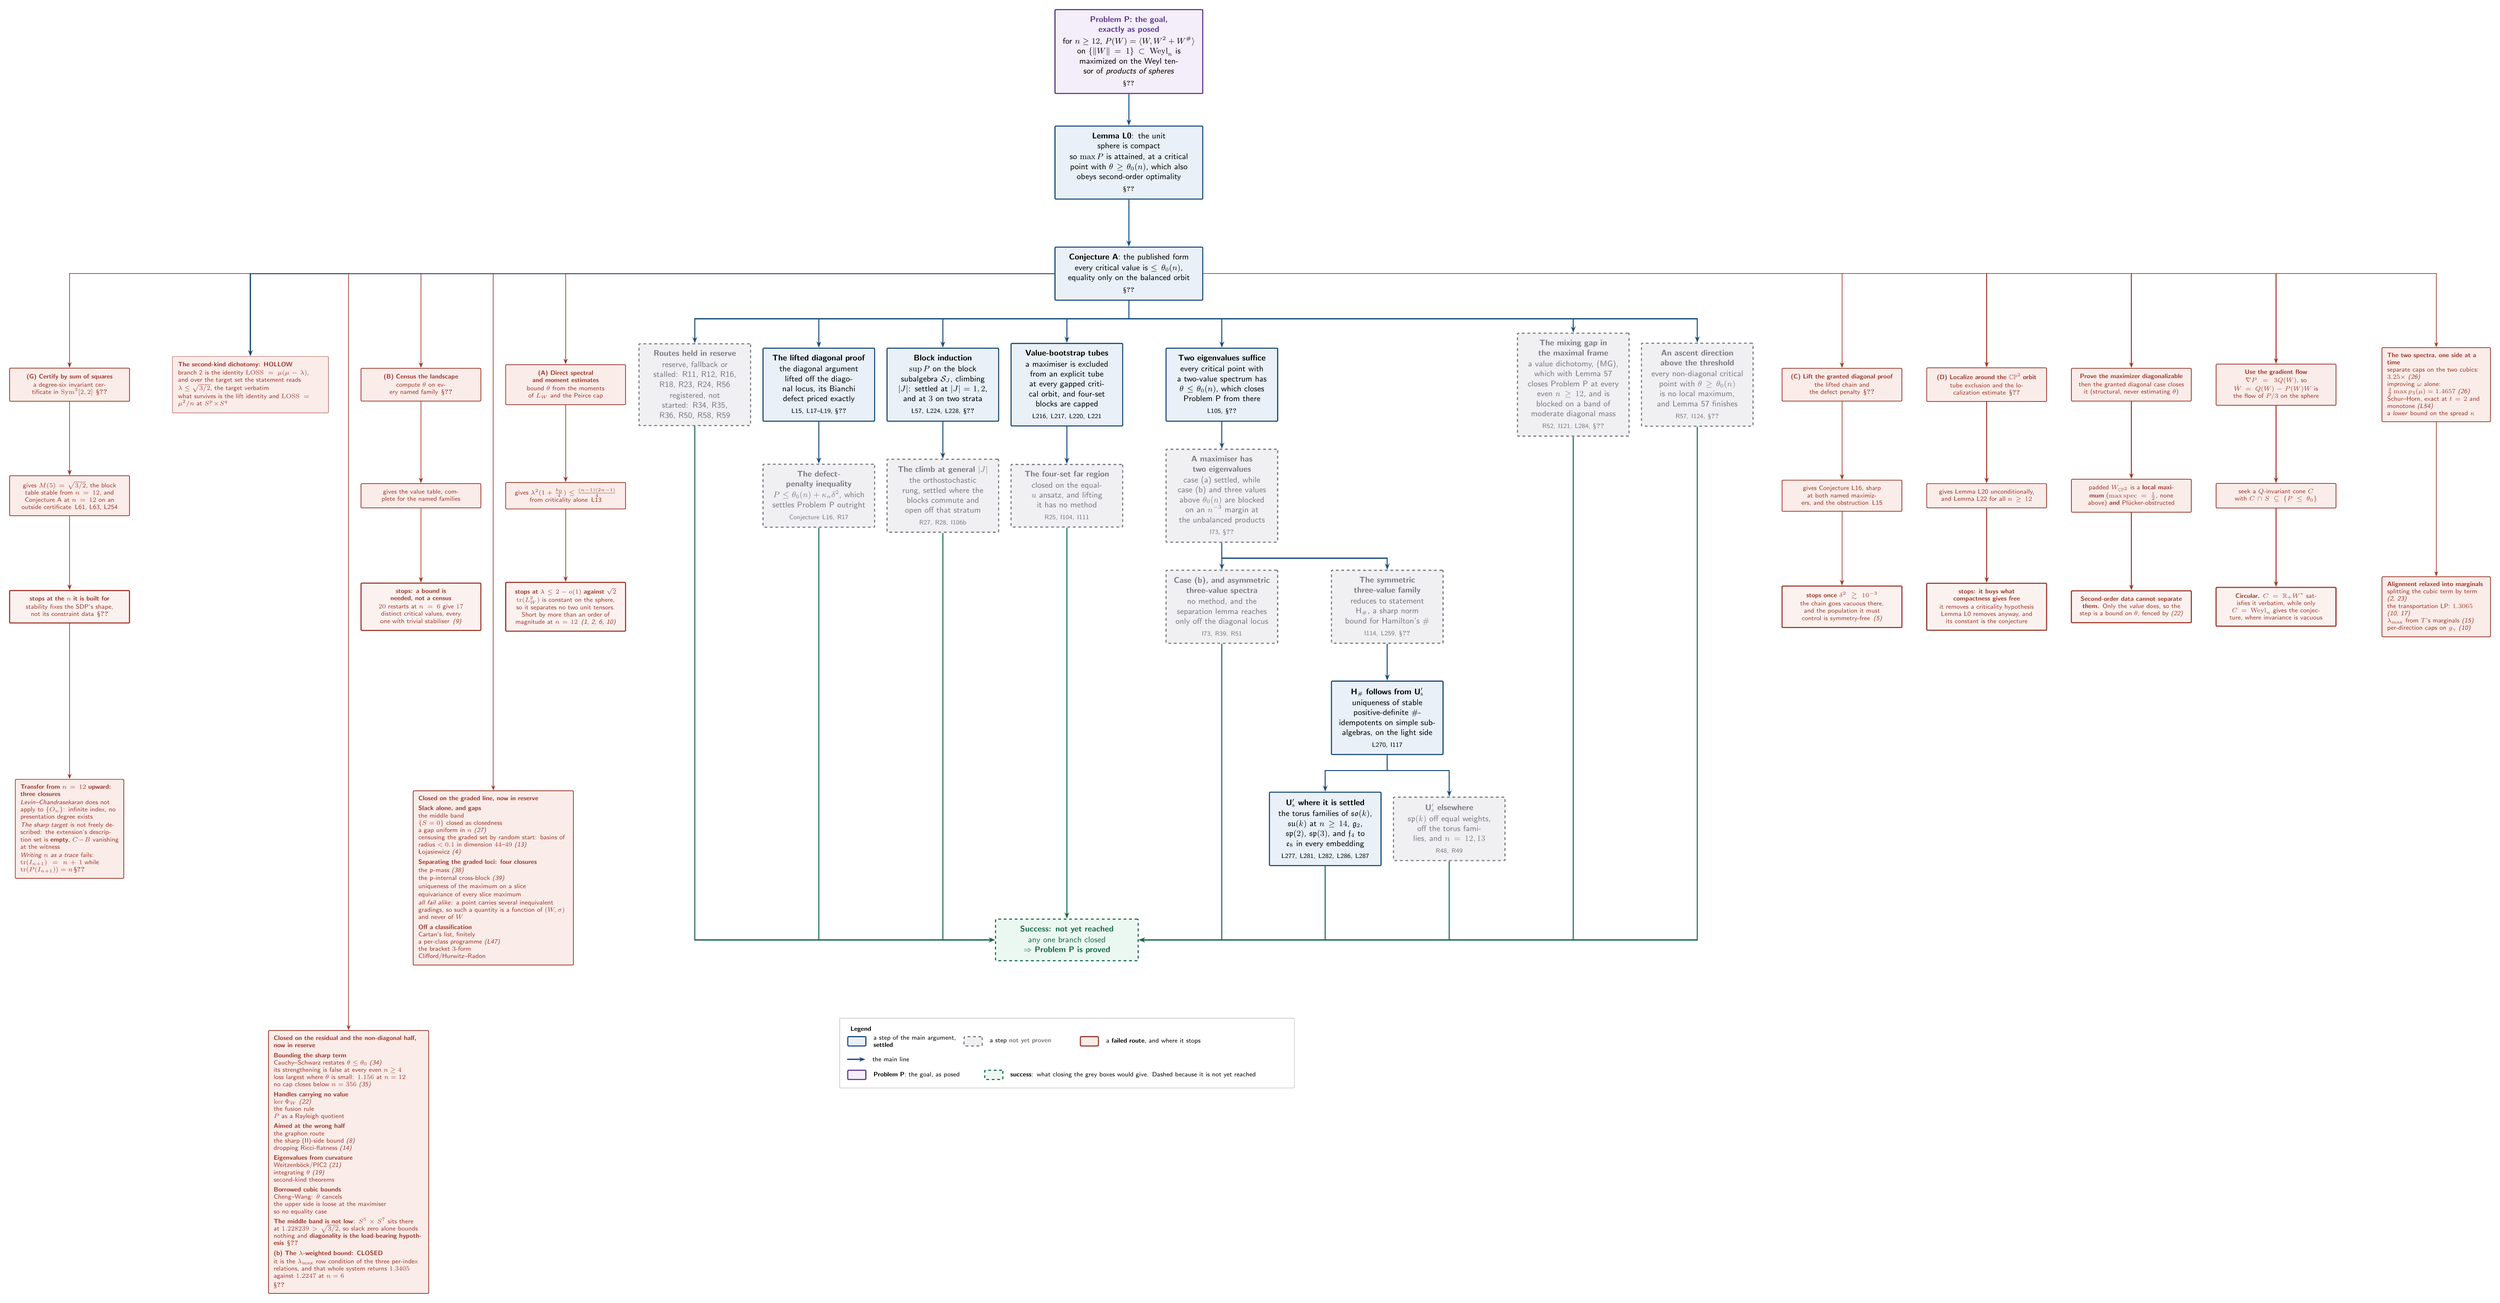
\begin{tikzpicture}[
  node distance=6mm and 9mm,
  font=\sffamily\small,
  spine/.style={draw=spineink, very thick, fill=spinebg, rounded corners=1pt,
                text width=62mm, align=center, inner sep=2.6mm},
  open/.style ={draw=openink, very thick, dashed, fill=openbg, rounded corners=1pt,
                text width=62mm, align=center, inner sep=2.6mm},
  stmt/.style ={draw=posedink, very thick, fill=posedbg, rounded corners=1pt,
                text width=76mm, align=center, inner sep=2.6mm},
  goal/.style ={draw=openink, very thick, dashed, fill=white, rounded corners=1pt,
                text width=76mm, align=center, inner sep=2.6mm},
  win/.style  ={draw=winink, very thick, dashed, fill=winbg, rounded corners=1pt,
                text width=76mm, align=center, inner sep=2.6mm},
  lem/.style  ={draw=lemink, fill=lembg, rounded corners=1pt,
                text width=40mm, align=left, inner sep=2.2mm, font=\sffamily\scriptsize},
  dead/.style ={draw=deadink, text=deadink, fill=deadbg, rounded corners=1pt,
                text width=40mm, align=left, inner sep=2.2mm, font=\sffamily\scriptsize},
  main/.style ={-{Stealth[length=2.4mm]}, spineink, very thick},
  feed/.style ={-{Stealth[length=2mm]}, lemink, dashed, thick},
  kill/.style ={-{Stealth[length=2mm]}, deadink, thick},
  failline/.style ={-{Stealth[length=2.2mm]}, deadink, thick},
  shut/.style ={draw=deadink, text=deadink, thick, fill=deadbg, rounded corners=1pt,
                align=center, inner sep=2.2mm, font=\sffamily\scriptsize},
  stop/.style ={draw=deadink, text=deadink, very thick, fill=deadbg!70, rounded corners=1pt,
                align=center, inner sep=2.2mm, font=\sffamily\scriptsize},
  side/.style ={draw=deadink, text=deadink, thick, fill=deadbg, rounded corners=1pt,
                align=left, inner sep=2.0mm, font=\sffamily\scriptsize},
]

% ===================== the live routes (Figure 1, copied verbatim into Figure 3) =====================
% One branch per live strategy under Conjecture A; routes that serve a single step
% fold into that step's box, and routes held in reserve share the grey box at left.
% Rows sit at the longest-path depth from Problem P, PITCH 43mm.
\node[stmt, text width=52mm] (asked) at (0mm,0mm)
      {\textbf{\color{posedink}Problem P: the goal, exactly as posed}\\[2pt]
       for $n\ge12$, $P(W)=\langle W,W^2+W^{\#}\rangle$ on $\{\|W\|=1\}\subset\Weyl_n$ is maximized on the Weyl tensor of \emph{products of spheres}\\[2pt] {\scriptsize\S\ref{sec:problem}}};
\node[spine, text width=52mm] (compact) at (0mm,-43mm)
      {\textbf{Lemma L0}: the unit sphere is compact\\[1pt] so $\max P$ is attained, at a critical point with $\theta\ge\theta_0(n)$, which also obeys second-order optimality\\[2pt] {\scriptsize\S\ref{sec:twoforms}}};
\node[spine, text width=52mm] (restate) at (0mm,-86mm)
      {\textbf{Conjecture A}: the published form\\[1pt] every critical value is $\le\theta_0(n)$, equality only on the balanced orbit\\[2pt] {\scriptsize\S\ref{sec:twoforms}}};

\node[open, text width=38mm] (reserve) at (-168mm,-129mm)
  {\textbf{\color{openink}Routes held in reserve}\\[1pt] \color{openink}reserve, fallback or stalled: R11, R12, R16, R18, R23, R24, R56\\[1pt] registered, not started: R34, R35, R36, R50, R58, R59};
\node[spine, text width=38mm] (lift) at (-120mm,-129mm)
  {\textbf{The lifted diagonal proof}\\[1pt] the diagonal argument lifted off the diagonal locus, its Bianchi defect priced exactly\\[2pt] {\scriptsize L15, L17--L19, \S\ref{app:C}}};
\node[spine, text width=38mm] (block) at (-72mm,-129mm)
  {\textbf{Block induction}\\[1pt] $\sup P$ on the block subalgebra $\mathcal S_J$, climbing $\lvert J\rvert$: settled at $\lvert J\rvert=1,2$, and at $3$ on two strata\\[2pt] {\scriptsize L57, L224, L228, \S\ref{sec:blockinduction}}};
\node[spine, text width=38mm] (tubes) at (-24mm,-129mm)
  {\textbf{Value-bootstrap tubes}\\[1pt] a maximiser is excluded from an explicit tube at every gapped critical orbit, and four-set blocks are capped\\[2pt] {\scriptsize L216, L217, L220, L221}};
\node[spine, text width=38mm] (twoval) at (36mm,-129mm)
  {\textbf{Two eigenvalues suffice}\\[1pt] every critical point with a two-value spectrum has $\theta\le\theta_0(n)$, which closes Problem~P from there\\[2pt] {\scriptsize L105, \S\ref{sec:classsystem}}};

\node[open, text width=38mm] (l16) at (-120mm,-172mm)
  {\textbf{\color{openink}The defect-penalty inequality}\\[1pt] \color{openink}$P\le\theta_0(n)+\kappa_n\delta^2$, which settles Problem~P outright\\[2pt] {\scriptsize Conjecture L16, R17}};
\node[open, text width=38mm] (climb) at (-72mm,-172mm)
  {\textbf{\color{openink}The climb at general $\lvert J\rvert$}\\[1pt] \color{openink}the orthostochastic rung, settled where the blocks commute and open off that stratum\\[2pt] {\scriptsize R27, R28, I106b}};
\node[open, text width=38mm] (far) at (-24mm,-172mm)
  {\textbf{\color{openink}The four-set far region}\\[1pt] \color{openink}closed on the equal-$u$ ansatz, and lifting it has no method\\[2pt] {\scriptsize R25, I104, I111}};
\node[open, text width=38mm] (i73) at (36mm,-172mm)
  {\textbf{\color{openink}A maximiser has two eigenvalues}\\[1pt] \color{openink}case (a) settled, while case (b) and three values above $\theta_0(n)$ are blocked on an $n^{-3}$ margin at the unbalanced products\\[2pt] {\scriptsize I73, \S\ref{sec:classsystem}}};

\node[open, text width=38mm] (asym) at (36mm,-215mm)
  {\textbf{\color{openink}Case (b), and asymmetric three-value spectra}\\[1pt] \color{openink}no method, and the separation lemma reaches only off the diagonal locus\\[2pt] {\scriptsize I73, R39, R51}};
\node[open, text width=38mm] (sym) at (100mm,-215mm)
  {\textbf{\color{openink}The symmetric three-value family}\\[1pt] \color{openink}reduces to statement H$_\#$, a sharp norm bound for Hamilton's $\#$\\[2pt] {\scriptsize I114, L259, \S\ref{sec:statementH}}};

\node[spine, text width=38mm] (hfromu) at (100mm,-258mm)
  {\textbf{H$_\#$ follows from U$_{\mathrm s}'$}\\[1pt] uniqueness of stable positive-definite $\#$-idempotents on simple subalgebras, on the light side\\[2pt] {\scriptsize L270, I117}};

\node[spine, text width=38mm] (torus) at (76mm,-301mm)
  {\textbf{U$_{\mathrm s}'$ where it is settled}\\[1pt] the torus families of $\mathfrak{so}(k)$, $\mathfrak{su}(k)$ at $n\ge14$, $\mathfrak g_2$, $\mathfrak{sp}(2)$, $\mathfrak{sp}(3)$, and $\mathfrak f_4$ to $\mathfrak e_8$ in every embedding\\[2pt] {\scriptsize L277, L281, L282, L286, L287}};
\node[open, text width=38mm] (offtorus) at (124mm,-301mm)
  {\textbf{\color{openink}U$_{\mathrm s}'$ elsewhere}\\[1pt] \color{openink}$\mathfrak{sp}(k)$ off equal weights, off the torus families, and $n=12,13$\\[2pt] {\scriptsize R48, R49}};

\node[open, text width=38mm] (mixgap) at (172mm,-129mm)
  {\textbf{\color{openink}The mixing gap in the maximal frame}\\[1pt] \color{openink}a value dichotomy, (MG), which with Lemma~57 closes Problem~P at every even $n\ge12$, and is blocked on a band of moderate diagonal mass\\[2pt] {\scriptsize R52, I121, L284, \S\ref{sec:mixinggap}}};

\node[open, text width=38mm] (ascent) at (220mm,-129mm)
  {\textbf{\color{openink}An ascent direction above the threshold}\\[1pt] \color{openink}every non-diagonal critical point with $\theta\ge\theta_0(n)$ is no local maximum, and Lemma~57 finishes\\[2pt] {\scriptsize R57, I124, \S\ref{sec:close}}};

\node[win, text width=50mm] (win) at (-24mm,-344mm)
  {\textbf{\color{winink}Success: not yet reached}\\[1pt] \color{winink}any one branch closed $\Rightarrow$ \textbf{Problem~P is proved}};

\draw[main] (asked) -- (compact);
\draw[main] (compact) -- (restate);
\draw[main] (restate.south) -- ++(0,-7mm) -| (reserve.north);
\draw[main] (restate.south) -- ++(0,-7mm) -| (lift.north);
\draw[main] (restate.south) -- ++(0,-7mm) -| (block.north);
\draw[main] (restate.south) -- ++(0,-7mm) -| (tubes.north);
\draw[main] (restate.south) -- ++(0,-7mm) -| (twoval.north);
\draw[main] (restate.south) -- ++(0,-7mm) -| (mixgap.north);
\draw[main] (restate.south) -- ++(0,-7mm) -| (ascent.north);
\draw[main] (lift) -- (l16);
\draw[main] (block) -- (climb);
\draw[main] (tubes) -- (far);
\draw[main] (twoval) -- (i73);
\draw[main] (i73) -- (asym);
\draw[main] (i73.south) -- ++(0,-6mm) -| (sym.north);
\draw[main] (sym) -- (hfromu);
\draw[main] (hfromu.south) -- ++(0,-6mm) -| (torus.north);
\draw[main] (hfromu.south) -- ++(0,-6mm) -| (offtorus.north);
\draw[main, winink] (reserve.south) |- (win.west);
\draw[main, winink] (l16.south) |- (win.west);
\draw[main, winink] (climb.south) |- (win.west);
\draw[main, winink] (far) -- (win);
\draw[main, winink] (asym.south) |- (win.east);
\draw[main, winink] (torus.south) |- (win.east);
\draw[main, winink] (offtorus.south) |- (win.east);
\draw[main, winink] (mixgap.south) |- (win.east);
\draw[main, winink] (ascent.south) |- (win.east);

% ===================== the failed routes, in red =====================
\node[shut, text width=42mm] (b1) at (-274mm,-129mm)
  {\textbf{(B) Census the landscape}\\[1pt] compute $\theta$ on every named family \,{\scriptsize\S\ref{app:census}}};
\node[shut, text width=42mm] (a1) at (-218mm,-129mm)
  {\textbf{(A) Direct spectral and moment estimates}\\[1pt] bound $\theta$ from the moments of $L_W$ and the Peirce cap};
\node[shut, text width=42mm] (c1) at (276mm,-129mm)
  {\textbf{(C) Lift the granted diagonal proof}\\[1pt] the lifted chain and the defect penalty \,{\scriptsize\S\ref{app:C}}};
\node[shut, text width=42mm] (d1) at (332mm,-129mm)
  {\textbf{(D) Localize around the $\CP^2$ orbit}\\[1pt] tube exclusion and the localization estimate \,{\scriptsize\S\ref{app:D}}};
\node[shut, text width=42mm] (b2) at (-274mm,-172mm)
  {gives the value table, complete for the named families};
\node[shut, text width=42mm] (a2) at (-218mm,-172mm)
  {gives $\lambda^2(1+\tfrac{k_0}4)\le\tfrac{(n-1)(2n-1)}4$ from criticality alone \,{\scriptsize L13}};
\node[shut, text width=42mm] (c2) at (276mm,-172mm)
  {gives Conjecture L16, sharp at both named maximizers, and the obstruction \,{\scriptsize L15}};
\node[shut, text width=42mm] (d2) at (332mm,-172mm)
  {gives Lemma L20 unconditionally, and Lemma L22 for all $n\ge12$};
\node[stop, text width=42mm] (b3) at (-274mm,-215mm)
  {\textbf{stops: a bound is needed, not a census}\\[1pt] $20$ restarts at $n=6$ give $17$ distinct critical values, every one with trivial stabiliser \,{\scriptsize\emph{(9)}}};
\node[stop, text width=42mm] (a3) at (-218mm,-215mm)
  {\textbf{stops at $\lambda\le2-o(1)$ against $\sqrt2$}\\[1pt] $\tr(L_W^2)$ is constant on the sphere, so it separates no two unit tensors. Short by more than an order of magnitude at $n=12$ \,{\scriptsize\emph{(1, 2, 6, 10)}}};
\node[stop, text width=42mm] (c3) at (276mm,-215mm)
  {\textbf{stops once $\delta^2\gtrsim10^{-3}$}\\[1pt] the chain goes vacuous there, and the population it must control is symmetry-free \,{\scriptsize\emph{(5)}}};
\node[stop, text width=42mm] (d3) at (332mm,-215mm)
  {\textbf{stops: it buys what compactness gives free}\\[1pt] it removes a criticality hypothesis Lemma L0 removes anyway, and its constant is the conjecture};
\node[side, text width=38mm] (s6) at (506mm,-129mm)
  {\textbf{The two spectra, one side at a time}\\ separate caps on the two cubics: $3.25\times$ \emph{(26)}\\ improving $\omega$ alone: $\tfrac32\max p_3(\mu)=1.4657$ \emph{(26)}\\ Schur--Horn, exact at $t=2$ and monotone \emph{(L54)}\\ a \emph{lower} bound on the spread $\kappa$};
\node[side, text width=38mm] (s7) at (506mm,-215mm)
  {\textbf{Alignment relaxed into marginals}\\ splitting the cubic term by term \emph{(2, 23)}\\ the transportation LP: $1.3065$ \emph{(10, 17)}\\ $\lambda_{\max}$ from $T$'s marginals \emph{(15)}\\ per-direction caps on $g_\gamma$ \emph{(10)}};
\node[shut, text width=42mm] (e1) at (388mm,-129mm)
  {\textbf{Prove the maximizer diagonalizable}\\[1pt] then the granted diagonal case closes it (structural, never estimating $\theta$)};
\node[shut, text width=42mm] (e2) at (388mm,-172mm)
  {padded $W_{\mathbb{CP}^2}$ is a \textbf{local maximum} ($\max\operatorname{spec}=\tfrac12$, none above) \textbf{and} Pl\"ucker-obstructed};
\node[stop, text width=42mm] (e3) at (388mm,-215mm)
  {\textbf{Second-order data cannot separate them.} Only the \emph{value} does, so the step is a bound on $\theta$, fenced by \emph{(22)}};
\node[shut, text width=42mm] (f1) at (444mm,-129mm)
  {\textbf{Use the gradient flow}\\[1pt] $\nabla P=3Q(W)$, so $\dot W=Q(W)-P(W)W$ is the flow of $P/3$ on the sphere};
\node[shut, text width=42mm] (f2) at (444mm,-172mm)
  {seek a $Q$-invariant cone $C$ with $C\cap S\subseteq\{P\le\theta_0\}$};
\node[stop, text width=42mm] (f3) at (444mm,-215mm)
  {\textbf{Circular.} $C=\mathbb R_+W^\ast$ satisfies it verbatim, while only $C=\mathrm{Weyl}_n$ gives the conjecture, where invariance is vacuous};
\node[dead, text width=56mm] (dich) at (-340mm,-129mm)
      {\textbf{\color{deadink}The second-kind dichotomy: HOLLOW}\\[1pt]
       \color{deadink}branch 2 is the identity $\mathrm{LOSS}=\mu(\mu-\lambda)$, and over the target set the statement reads $\lambda\le\sqrt{3/2}$, the target verbatim\\[1pt]
       \color{deadink}what survives is the lift identity and $\mathrm{LOSS}=\mu^2/n$ at $S^p\!\times\!S^q$};

\node[shut, text width=42mm] (g1) at (-410mm,-129mm)
  {\textbf{(G) Certify by sum of squares}\\[1pt] a degree-six invariant certificate in $\mathrm{Sym}^3[2,2]$ \,{\scriptsize\S\ref{sec:sos}}};
\node[shut, text width=42mm] (g2) at (-410mm,-172mm)
  {gives $M(5)=\sqrt{3/2}$, the block table stable from $n=12$, and Conjecture~A at $n=12$ on an outside certificate \,{\scriptsize L61, L63, L254}};
\node[stop, text width=42mm] (g3) at (-410mm,-215mm)
  {\textbf{stops at the $n$ it is built for}\\[1pt] stability fixes the SDP's shape, not its constraint data \,{\scriptsize\S\ref{sec:sos12}}};
\node[side, text width=38mm] (transferdead) at (-410mm,-301mm)
  {\textbf{Transfer from $n=12$ upward: three closures}\\[1pt] \emph{Levin--Chandrasekaran} does not apply to $\{O_n\}$: infinite index, no presentation degree exists\\[1pt] \emph{The sharp target} is not freely described: the extension's description set is \textbf{empty}, $C-B$ vanishing at the witness\\[1pt] \emph{Writing $n$ as a trace} fails: $\mathrm{tr}(I_{n+1})=n+1$ while $\mathrm{tr}(P(I_{n+1}))=n$\,{\S\ref{sec:sos12}}};
\node[side, text width=58mm] (rgraded) at (-246mm,-320mm)
  {\textbf{Closed on the graded line, now in reserve}\\[3pt] \textbf{Slack alone, and gaps}\\ the middle band\\ $\{S=0\}$ closed as closedness\\ a gap uniform in $n$ \emph{(27)}\\ censusing the graded set by random start: basins of radius $<0.1$ in dimension $44$--$49$ \emph{(13)}\\ {\L}ojasiewicz \emph{(4)}\\[3pt] \textbf{Separating the graded loci: four closures}\\[1pt] the $\pp$-mass \emph{(38)}\\[1pt] the $\pp$-internal cross-block \emph{(39)}\\[1pt] uniqueness of the maximum on a slice\\[1pt] equivariance of every slice maximum\\[1pt] \emph{all fail alike}: a point carries several inequivalent gradings, so such a quantity is a function of $(W,\sigma)$ and never of $W$\\[3pt] \textbf{Off a classification}\\ Cartan's list, finitely\\ a per-class programme \emph{(L47)}\\ the bracket $3$-form\\ Clifford/Hurwitz--Radon};
\node[side, text width=58mm] (rresid) at (-302mm,-430mm)
  {\textbf{Closed on the residual and the non-diagonal half, now in reserve}\\[3pt] \textbf{Bounding the sharp term}\\ Cauchy--Schwarz restates $\theta\le\theta_0$ \emph{(34)}\\ its strengthening is false at every even $n\ge4$\\ loss largest where $\theta$ is small: $1.156$ at $n=12$\\ no cap closes below $n=356$ \emph{(35)}\\[3pt] \textbf{Handles carrying no value}\\ $\ker\Phi_W$ \emph{(22)}\\ the fusion rule\\ $P$ as a Rayleigh quotient\\[3pt] \textbf{Aimed at the wrong half}\\ the graphon route\\ the sharp (II)-side bound \emph{(8)}\\ dropping Ricci-flatness \emph{(14)}\\[3pt] \textbf{Eigenvalues from curvature}\\ Weitzenb\"ock/PIC2 \emph{(21)}\\ integrating $\theta$ \emph{(19)}\\ second-kind theorems\\[3pt] \textbf{Borrowed cubic bounds}\\ Cheng--Wang: $\theta$ cancels\\ the upper side is loose at the maximiser\\ so no equality case\\[3pt] \textbf{The middle band is not low}: $S^5\times S^7$ sits there at $1.228239>\sqrt{3/2}$, so slack zero alone bounds nothing and \textbf{diagonality is the load-bearing hypothesis} \,{\S\ref{sec:horns}}\\[3pt] \textbf{\color{deadink}(b) The $\lambda$-weighted bound: CLOSED}\\[1pt] \color{deadink}it is the $\lambda_{\max}$ row condition of the three per-index relations, and that whole system returns $1.3405$ against $1.2247$ at $n=6$\\[2pt] {\scriptsize\S\ref{sec:pinned}}};

\draw[failline] (restate.west) -- ++(-40mm,0) -| (a1.north);
\draw[failline] (restate.west) -- ++(-40mm,0) -| (b1.north);
\draw[failline] (restate.east) -- ++(40mm,0) -| (c1.north);
\draw[failline] (restate.east) -- ++(40mm,0) -| (d1.north);
\draw[failline] (a1) -- (a2);  \draw[failline] (a2) -- (a3);
\draw[failline] (b1) -- (b2);  \draw[failline] (b2) -- (b3);
\draw[failline] (c1) -- (c2);  \draw[failline] (c2) -- (c3);
\draw[failline] (d1) -- (d2);  \draw[failline] (d2) -- (d3);
\draw[failline] (restate.east) -- ++(40mm,0) -| (e1.north);
\draw[failline] (restate.east) -- ++(40mm,0) -| (f1.north);
\draw[failline] (e1) -- (e2);  \draw[failline] (e2) -- (e3);
\draw[failline] (f1) -- (f2);  \draw[failline] (f2) -- (f3);
\draw[failline] (restate.west) -- ++(-40mm,0) -| (g1.north);
\draw[failline] (g1) -- (g2);  \draw[failline] (g2) -- (g3);
\draw[main] (restate.west) -- ++(-30mm,0) -| (dich.north);
\draw[kill] (restate.east) -- ++(46mm,0) -| (s6.north);
\draw[kill] (s6.south) -- (s7.north);
\draw[kill] (g3.south) -- (transferdead.north);
\draw[kill] (restate.west) -- ++(-40mm,0) -| (rgraded.north);
\draw[kill] (restate.west) -- ++(-40mm,0) -| (rresid.north);

% ---------------- legend
\begin{scope}[shift={($(win.south)+(-88mm,-22mm)$)}, font=\sffamily\scriptsize]
  \node[draw=black!35, fill=white, rounded corners=1pt, inner sep=3mm,
        minimum width=176mm, minimum height=27mm, anchor=north west] (leg) at (0,0) {};
  \node[anchor=north west, font=\sffamily\scriptsize\bfseries] at ($(leg.north west)+(3mm,-2mm)$) {Legend};

  \node[draw=spineink, very thick, fill=spinebg, rounded corners=1pt,
        minimum width=7mm, minimum height=3.6mm, anchor=west] (k1) at ($(leg.north west)+(3mm,-9mm)$) {};
  \node[anchor=west, text width=34mm] at ($(k1.east)+(1.5mm,0)$) {a step of the main argument, \textbf{settled}};

  \node[draw=openink, very thick, dashed, fill=openbg, rounded corners=1pt,
        minimum width=7mm, minimum height=3.6mm, anchor=west] (k2) at ($(leg.north west)+(48mm,-9mm)$) {};
  \node[anchor=west, text width=34mm] at ($(k2.east)+(1.5mm,0)$) {a step \textbf{\color{openink}not yet proven}};

  \node[draw=deadink, very thick, fill=deadbg, rounded corners=1pt,
        minimum width=7mm, minimum height=3.6mm, anchor=west] (k4) at ($(leg.north west)+(93mm,-9mm)$) {};
  \node[anchor=west, text width=40mm] at ($(k4.east)+(1.5mm,0)$) {a \textbf{failed route}, and where it stops};


  \node[draw=posedink, very thick, fill=posedbg, rounded corners=1pt,
        minimum width=7mm, minimum height=3.6mm, anchor=west] (k5) at ($(leg.north west)+(3mm,-22mm)$) {};
  \node[anchor=west, text width=42mm] at ($(k5.east)+(1.5mm,0)$) {\textbf{Problem P}: the goal, as posed};

  \node[draw=winink, very thick, dashed, fill=winbg, rounded corners=1pt,
        minimum width=7mm, minimum height=3.6mm, anchor=west] (k6) at ($(leg.north west)+(56mm,-22mm)$) {};
  \node[anchor=west, text width=110mm] at ($(k6.east)+(1.5mm,0)$) {\textbf{success}: what closing the grey boxes would give. Dashed because it is not yet reached};



  \draw[main] ($(leg.north west)+(3mm,-16mm)$) -- ++(7mm,0);
  \node[anchor=west, text width=34mm] at ($(leg.north west)+(11.5mm,-16mm)$) {the main line};


\end{scope}

\end{tikzpicture}%
}
\caption{\textbf{The same map, with the failed routes in red.} The centre is Figure~\ref{fig:routes} (the live routes) together with the second-kind dichotomy, which is hollow on the target set and so appears here rather than there. Seven strategies fork from Conjecture~A as red branches, each running to what it produced and then to where it stops, and none reaches the success box. A red box beside a step is a closure that bites that one step rather than a whole route, and the two hanging from Conjecture~A collect the closures on steps of routes now held in reserve. A parenthesised number is the fence post that holds it in \S\ref{sec:fenceposts}, an $L$ the lemma. A failed route is a result: each red terminus states what a new attempt must clear. \textbf{Figure~\ref{fig:closed-dag} reads what the results named here rest on.}}
\label{fig:closed}
\end{sidewaysfigure}

\clearpage
% GENERATED by scripts/misc/result_dag_figures.py -- do not edit
\begin{figure}[H]
\centering
\begin{adjustbox}{max width=\textwidth, max totalheight=0.78\textheight}
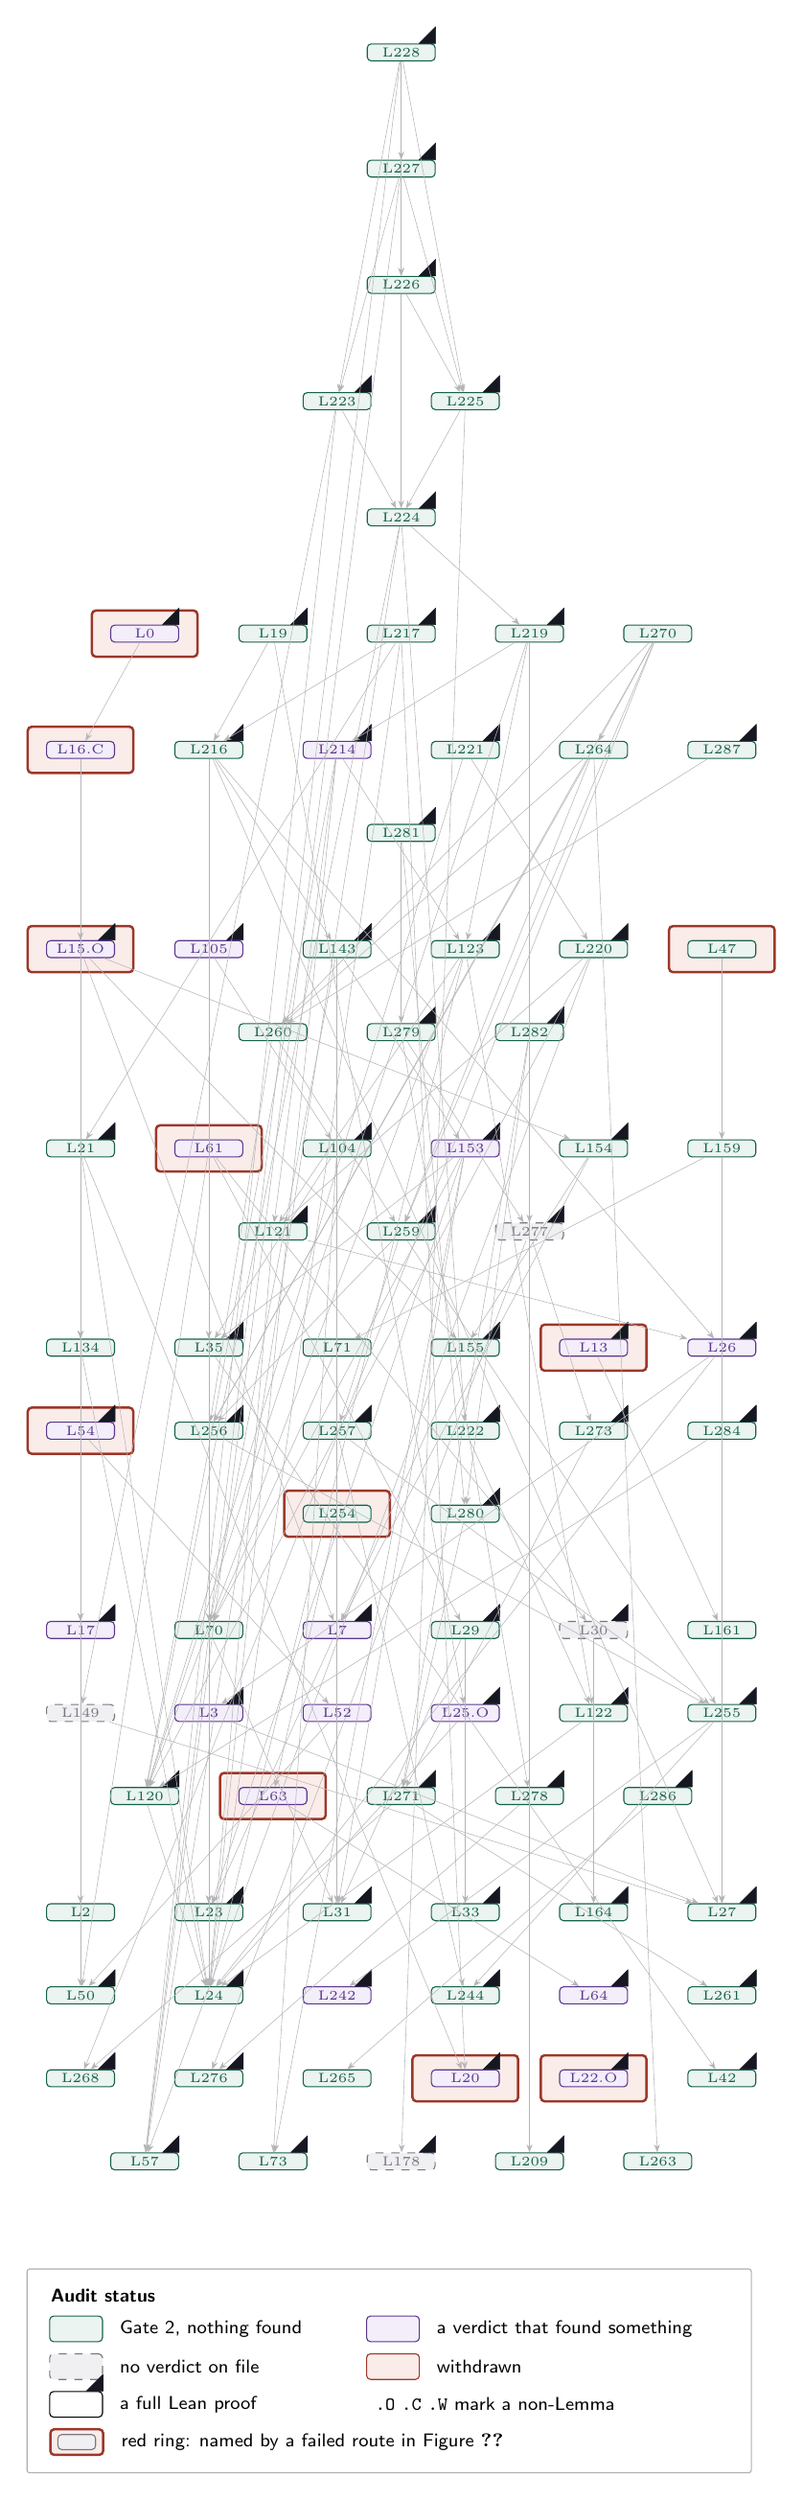
\begin{tikzpicture}[
  x=17mm,y=11mm,
  every node/.style={font=\tiny},
  res/.style={draw,rounded corners=1.5pt,inner sep=1.5pt,minimum width=9mm,align=center},
  ok/.style={res,draw=lemink,fill=lembg,text=lemink},
  gap/.style={res,draw=posedink,fill=posedbg,text=posedink},
  raw/.style={res,draw=openink,fill=openbg,text=openink,dashed},
  gone/.style={res,draw=deadink,fill=deadbg,text=deadink},
  halo/.style={res,draw=deadink,fill=deadbg,text=deadbg,inner xsep=9pt,inner ysep=7pt,minimum width=14mm,line width=.9pt},
  dep/.style={-{Stealth[length=3pt]},openink!55,line width=.2pt},
  bad/.style={-{Stealth[length=3pt]},deadink,line width=.5pt},
  lean/.style={fill=inkline,draw=inkline,line width=.2pt,line join=round},
]
\node[halo] at (-2.00,-7.00) {L0};
\node[halo] at (1.50,-15.60) {L13};
\node[halo] at (-2.50,-10.80) {L15.O};
\node[halo] at (-2.50,-8.40) {L16.C};
\node[halo] at (0.50,-24.40) {L20};
\node[halo] at (1.50,-24.40) {L22.O};
\node[halo] at (2.50,-10.80) {L47};
\node[halo] at (-2.50,-16.60) {L54};
\node[halo] at (-1.50,-13.20) {L61};
\node[halo] at (-1.00,-21.00) {L63};
\node[halo] at (-0.50,-17.60) {L254};
\node[gap] (n0) at (-2.00,-7.00) {L0};
\node[ok] (n2) at (-2.50,-22.40) {L2};
\node[gap] (n3) at (-1.50,-20.00) {L3};
\node[gap] (n7) at (-0.50,-19.00) {L7};
\node[gap] (n13) at (1.50,-15.60) {L13};
\node[gap] (n15) at (-2.50,-10.80) {L15.O};
\node[gap] (n16) at (-2.50,-8.40) {L16.C};
\node[gap] (n17) at (-2.50,-19.00) {L17};
\node[ok] (n19) at (-1.00,-7.00) {L19};
\node[gap] (n20) at (0.50,-24.40) {L20};
\node[ok] (n21) at (-2.50,-13.20) {L21};
\node[gap] (n22) at (1.50,-24.40) {L22.O};
\node[ok] (n23) at (-1.50,-22.40) {L23};
\node[ok] (n24) at (-1.50,-23.40) {L24};
\node[gap] (n25) at (0.50,-20.00) {L25.O};
\node[gap] (n26) at (2.50,-15.60) {L26};
\node[ok] (n27) at (2.50,-22.40) {L27};
\node[ok] (n29) at (0.50,-19.00) {L29};
\node[raw] (n30) at (1.50,-19.00) {L30};
\node[ok] (n31) at (-0.50,-22.40) {L31};
\node[ok] (n33) at (0.50,-22.40) {L33};
\node[ok] (n35) at (-1.50,-15.60) {L35};
\node[ok] (n42) at (2.50,-24.40) {L42};
\node[ok] (n47) at (2.50,-10.80) {L47};
\node[ok] (n50) at (-2.50,-23.40) {L50};
\node[gap] (n52) at (-0.50,-20.00) {L52};
\node[gap] (n54) at (-2.50,-16.60) {L54};
\node[ok] (n57) at (-2.00,-25.40) {L57};
\node[gap] (n61) at (-1.50,-13.20) {L61};
\node[gap] (n63) at (-1.00,-21.00) {L63};
\node[gap] (n64) at (1.50,-23.40) {L64};
\node[ok] (n70) at (-1.50,-19.00) {L70};
\node[ok] (n71) at (-0.50,-15.60) {L71};
\node[ok] (n73) at (-1.00,-25.40) {L73};
\node[ok] (n104) at (-0.50,-13.20) {L104};
\node[gap] (n105) at (-1.50,-10.80) {L105};
\node[ok] (n120) at (-2.00,-21.00) {L120};
\node[ok] (n121) at (-1.00,-14.20) {L121};
\node[ok] (n122) at (1.50,-20.00) {L122};
\node[ok] (n123) at (0.50,-10.80) {L123};
\node[ok] (n134) at (-2.50,-15.60) {L134};
\node[ok] (n143) at (-0.50,-10.80) {L143};
\node[raw] (n149) at (-2.50,-20.00) {L149};
\node[gap] (n153) at (0.50,-13.20) {L153};
\node[ok] (n154) at (1.50,-13.20) {L154};
\node[ok] (n155) at (0.50,-15.60) {L155};
\node[ok] (n159) at (2.50,-13.20) {L159};
\node[ok] (n161) at (2.50,-19.00) {L161};
\node[ok] (n164) at (1.50,-22.40) {L164};
\node[raw] (n178) at (0.00,-25.40) {L178};
\node[ok] (n209) at (1.00,-25.40) {L209};
\node[gap] (n214) at (-0.50,-8.40) {L214};
\node[ok] (n216) at (-1.50,-8.40) {L216};
\node[ok] (n217) at (0.00,-7.00) {L217};
\node[ok] (n219) at (1.00,-7.00) {L219};
\node[ok] (n220) at (1.50,-10.80) {L220};
\node[ok] (n221) at (0.50,-8.40) {L221};
\node[ok] (n222) at (0.50,-16.60) {L222};
\node[ok] (n223) at (-0.50,-4.20) {L223};
\node[ok] (n224) at (0.00,-5.60) {L224};
\node[ok] (n225) at (0.50,-4.20) {L225};
\node[ok] (n226) at (0.00,-2.80) {L226};
\node[ok] (n227) at (0.00,-1.40) {L227};
\node[ok] (n228) at (0.00,0.00) {L228};
\node[gap] (n242) at (-0.50,-23.40) {L242};
\node[ok] (n244) at (0.50,-23.40) {L244};
\node[ok] (n254) at (-0.50,-17.60) {L254};
\node[ok] (n255) at (2.50,-20.00) {L255};
\node[ok] (n256) at (-1.50,-16.60) {L256};
\node[ok] (n257) at (-0.50,-16.60) {L257};
\node[ok] (n259) at (0.00,-14.20) {L259};
\node[ok] (n260) at (-1.00,-11.80) {L260};
\node[ok] (n261) at (2.50,-23.40) {L261};
\node[ok] (n263) at (2.00,-25.40) {L263};
\node[ok] (n264) at (1.50,-8.40) {L264};
\node[ok] (n265) at (-0.50,-24.40) {L265};
\node[ok] (n268) at (-2.50,-24.40) {L268};
\node[ok] (n270) at (2.00,-7.00) {L270};
\node[ok] (n271) at (0.00,-21.00) {L271};
\node[ok] (n273) at (1.50,-16.60) {L273};
\node[ok] (n276) at (-1.50,-24.40) {L276};
\node[raw] (n277) at (1.00,-14.20) {L277};
\node[ok] (n278) at (1.00,-21.00) {L278};
\node[ok] (n279) at (0.00,-11.80) {L279};
\node[ok] (n280) at (0.50,-17.60) {L280};
\node[ok] (n281) at (0.00,-9.40) {L281};
\node[ok] (n282) at (1.00,-11.80) {L282};
\node[ok] (n284) at (2.50,-16.60) {L284};
\node[ok] (n286) at (2.00,-21.00) {L286};
\node[ok] (n287) at (2.50,-8.40) {L287};
\fill[lean] (n0.north east) -- ++(-2.2mm,0) -- ++(2.2mm,2.2mm) -- cycle;
\fill[lean] (n3.north east) -- ++(-2.2mm,0) -- ++(2.2mm,2.2mm) -- cycle;
\fill[lean] (n7.north east) -- ++(-2.2mm,0) -- ++(2.2mm,2.2mm) -- cycle;
\fill[lean] (n13.north east) -- ++(-2.2mm,0) -- ++(2.2mm,2.2mm) -- cycle;
\fill[lean] (n15.north east) -- ++(-2.2mm,0) -- ++(2.2mm,2.2mm) -- cycle;
\fill[lean] (n17.north east) -- ++(-2.2mm,0) -- ++(2.2mm,2.2mm) -- cycle;
\fill[lean] (n19.north east) -- ++(-2.2mm,0) -- ++(2.2mm,2.2mm) -- cycle;
\fill[lean] (n20.north east) -- ++(-2.2mm,0) -- ++(2.2mm,2.2mm) -- cycle;
\fill[lean] (n21.north east) -- ++(-2.2mm,0) -- ++(2.2mm,2.2mm) -- cycle;
\fill[lean] (n22.north east) -- ++(-2.2mm,0) -- ++(2.2mm,2.2mm) -- cycle;
\fill[lean] (n23.north east) -- ++(-2.2mm,0) -- ++(2.2mm,2.2mm) -- cycle;
\fill[lean] (n24.north east) -- ++(-2.2mm,0) -- ++(2.2mm,2.2mm) -- cycle;
\fill[lean] (n25.north east) -- ++(-2.2mm,0) -- ++(2.2mm,2.2mm) -- cycle;
\fill[lean] (n26.north east) -- ++(-2.2mm,0) -- ++(2.2mm,2.2mm) -- cycle;
\fill[lean] (n27.north east) -- ++(-2.2mm,0) -- ++(2.2mm,2.2mm) -- cycle;
\fill[lean] (n29.north east) -- ++(-2.2mm,0) -- ++(2.2mm,2.2mm) -- cycle;
\fill[lean] (n30.north east) -- ++(-2.2mm,0) -- ++(2.2mm,2.2mm) -- cycle;
\fill[lean] (n31.north east) -- ++(-2.2mm,0) -- ++(2.2mm,2.2mm) -- cycle;
\fill[lean] (n33.north east) -- ++(-2.2mm,0) -- ++(2.2mm,2.2mm) -- cycle;
\fill[lean] (n35.north east) -- ++(-2.2mm,0) -- ++(2.2mm,2.2mm) -- cycle;
\fill[lean] (n42.north east) -- ++(-2.2mm,0) -- ++(2.2mm,2.2mm) -- cycle;
\fill[lean] (n50.north east) -- ++(-2.2mm,0) -- ++(2.2mm,2.2mm) -- cycle;
\fill[lean] (n54.north east) -- ++(-2.2mm,0) -- ++(2.2mm,2.2mm) -- cycle;
\fill[lean] (n57.north east) -- ++(-2.2mm,0) -- ++(2.2mm,2.2mm) -- cycle;
\fill[lean] (n64.north east) -- ++(-2.2mm,0) -- ++(2.2mm,2.2mm) -- cycle;
\fill[lean] (n73.north east) -- ++(-2.2mm,0) -- ++(2.2mm,2.2mm) -- cycle;
\fill[lean] (n104.north east) -- ++(-2.2mm,0) -- ++(2.2mm,2.2mm) -- cycle;
\fill[lean] (n105.north east) -- ++(-2.2mm,0) -- ++(2.2mm,2.2mm) -- cycle;
\fill[lean] (n120.north east) -- ++(-2.2mm,0) -- ++(2.2mm,2.2mm) -- cycle;
\fill[lean] (n121.north east) -- ++(-2.2mm,0) -- ++(2.2mm,2.2mm) -- cycle;
\fill[lean] (n122.north east) -- ++(-2.2mm,0) -- ++(2.2mm,2.2mm) -- cycle;
\fill[lean] (n123.north east) -- ++(-2.2mm,0) -- ++(2.2mm,2.2mm) -- cycle;
\fill[lean] (n143.north east) -- ++(-2.2mm,0) -- ++(2.2mm,2.2mm) -- cycle;
\fill[lean] (n153.north east) -- ++(-2.2mm,0) -- ++(2.2mm,2.2mm) -- cycle;
\fill[lean] (n154.north east) -- ++(-2.2mm,0) -- ++(2.2mm,2.2mm) -- cycle;
\fill[lean] (n155.north east) -- ++(-2.2mm,0) -- ++(2.2mm,2.2mm) -- cycle;
\fill[lean] (n164.north east) -- ++(-2.2mm,0) -- ++(2.2mm,2.2mm) -- cycle;
\fill[lean] (n178.north east) -- ++(-2.2mm,0) -- ++(2.2mm,2.2mm) -- cycle;
\fill[lean] (n209.north east) -- ++(-2.2mm,0) -- ++(2.2mm,2.2mm) -- cycle;
\fill[lean] (n214.north east) -- ++(-2.2mm,0) -- ++(2.2mm,2.2mm) -- cycle;
\fill[lean] (n216.north east) -- ++(-2.2mm,0) -- ++(2.2mm,2.2mm) -- cycle;
\fill[lean] (n217.north east) -- ++(-2.2mm,0) -- ++(2.2mm,2.2mm) -- cycle;
\fill[lean] (n219.north east) -- ++(-2.2mm,0) -- ++(2.2mm,2.2mm) -- cycle;
\fill[lean] (n220.north east) -- ++(-2.2mm,0) -- ++(2.2mm,2.2mm) -- cycle;
\fill[lean] (n221.north east) -- ++(-2.2mm,0) -- ++(2.2mm,2.2mm) -- cycle;
\fill[lean] (n222.north east) -- ++(-2.2mm,0) -- ++(2.2mm,2.2mm) -- cycle;
\fill[lean] (n223.north east) -- ++(-2.2mm,0) -- ++(2.2mm,2.2mm) -- cycle;
\fill[lean] (n224.north east) -- ++(-2.2mm,0) -- ++(2.2mm,2.2mm) -- cycle;
\fill[lean] (n225.north east) -- ++(-2.2mm,0) -- ++(2.2mm,2.2mm) -- cycle;
\fill[lean] (n226.north east) -- ++(-2.2mm,0) -- ++(2.2mm,2.2mm) -- cycle;
\fill[lean] (n227.north east) -- ++(-2.2mm,0) -- ++(2.2mm,2.2mm) -- cycle;
\fill[lean] (n228.north east) -- ++(-2.2mm,0) -- ++(2.2mm,2.2mm) -- cycle;
\fill[lean] (n242.north east) -- ++(-2.2mm,0) -- ++(2.2mm,2.2mm) -- cycle;
\fill[lean] (n244.north east) -- ++(-2.2mm,0) -- ++(2.2mm,2.2mm) -- cycle;
\fill[lean] (n255.north east) -- ++(-2.2mm,0) -- ++(2.2mm,2.2mm) -- cycle;
\fill[lean] (n256.north east) -- ++(-2.2mm,0) -- ++(2.2mm,2.2mm) -- cycle;
\fill[lean] (n257.north east) -- ++(-2.2mm,0) -- ++(2.2mm,2.2mm) -- cycle;
\fill[lean] (n259.north east) -- ++(-2.2mm,0) -- ++(2.2mm,2.2mm) -- cycle;
\fill[lean] (n261.north east) -- ++(-2.2mm,0) -- ++(2.2mm,2.2mm) -- cycle;
\fill[lean] (n268.north east) -- ++(-2.2mm,0) -- ++(2.2mm,2.2mm) -- cycle;
\fill[lean] (n271.north east) -- ++(-2.2mm,0) -- ++(2.2mm,2.2mm) -- cycle;
\fill[lean] (n273.north east) -- ++(-2.2mm,0) -- ++(2.2mm,2.2mm) -- cycle;
\fill[lean] (n276.north east) -- ++(-2.2mm,0) -- ++(2.2mm,2.2mm) -- cycle;
\fill[lean] (n277.north east) -- ++(-2.2mm,0) -- ++(2.2mm,2.2mm) -- cycle;
\fill[lean] (n278.north east) -- ++(-2.2mm,0) -- ++(2.2mm,2.2mm) -- cycle;
\fill[lean] (n279.north east) -- ++(-2.2mm,0) -- ++(2.2mm,2.2mm) -- cycle;
\fill[lean] (n280.north east) -- ++(-2.2mm,0) -- ++(2.2mm,2.2mm) -- cycle;
\fill[lean] (n281.north east) -- ++(-2.2mm,0) -- ++(2.2mm,2.2mm) -- cycle;
\fill[lean] (n282.north east) -- ++(-2.2mm,0) -- ++(2.2mm,2.2mm) -- cycle;
\fill[lean] (n284.north east) -- ++(-2.2mm,0) -- ++(2.2mm,2.2mm) -- cycle;
\fill[lean] (n286.north east) -- ++(-2.2mm,0) -- ++(2.2mm,2.2mm) -- cycle;
\fill[lean] (n287.north east) -- ++(-2.2mm,0) -- ++(2.2mm,2.2mm) -- cycle;
\draw[dep] (n0) -- (n16);
\draw[dep] (n3) -- (n24);
\draw[dep] (n3) -- (n27);
\draw[dep] (n7) -- (n23);
\draw[dep] (n13) -- (n161);
\draw[dep] (n15) -- (n7);
\draw[dep] (n15) -- (n154);
\draw[dep] (n15) -- (n155);
\draw[dep] (n16) -- (n15);
\draw[dep] (n16) -- (n17);
\draw[dep] (n16) -- (n134);
\draw[dep] (n17) -- (n2);
\draw[dep] (n19) -- (n25);
\draw[dep] (n19) -- (n216);
\draw[dep] (n21) -- (n20);
\draw[dep] (n21) -- (n24);
\draw[dep] (n21) -- (n134);
\draw[dep] (n25) -- (n24);
\draw[dep] (n26) -- (n3);
\draw[dep] (n26) -- (n24);
\draw[dep] (n26) -- (n27);
\draw[dep] (n29) -- (n31);
\draw[dep] (n29) -- (n33);
\draw[dep] (n30) -- (n164);
\draw[dep] (n35) -- (n42);
\draw[dep] (n35) -- (n70);
\draw[dep] (n47) -- (n159);
\draw[dep] (n52) -- (n50);
\draw[dep] (n54) -- (n50);
\draw[dep] (n54) -- (n52);
\draw[dep] (n61) -- (n29);
\draw[dep] (n61) -- (n30);
\draw[dep] (n61) -- (n35);
\draw[dep] (n61) -- (n50);
\draw[dep] (n63) -- (n64);
\draw[dep] (n70) -- (n23);
\draw[dep] (n70) -- (n31);
\draw[dep] (n71) -- (n70);
\draw[dep] (n104) -- (n31);
\draw[dep] (n104) -- (n35);
\draw[dep] (n104) -- (n73);
\draw[dep] (n105) -- (n23);
\draw[dep] (n105) -- (n104);
\draw[dep] (n120) -- (n24);
\draw[dep] (n121) -- (n24);
\draw[dep] (n121) -- (n26);
\draw[dep] (n122) -- (n24);
\draw[dep] (n123) -- (n24);
\draw[dep] (n123) -- (n120);
\draw[dep] (n123) -- (n121);
\draw[dep] (n123) -- (n122);
\draw[dep] (n134) -- (n17);
\draw[dep] (n134) -- (n24);
\draw[dep] (n143) -- (n31);
\draw[dep] (n143) -- (n70);
\draw[dep] (n143) -- (n153);
\draw[dep] (n149) -- (n27);
\draw[dep] (n153) -- (n23);
\draw[dep] (n153) -- (n31);
\draw[dep] (n153) -- (n35);
\draw[dep] (n153) -- (n70);
\draw[dep] (n153) -- (n73);
\draw[dep] (n154) -- (n7);
\draw[dep] (n154) -- (n155);
\draw[dep] (n155) -- (n7);
\draw[dep] (n159) -- (n27);
\draw[dep] (n159) -- (n71);
\draw[dep] (n161) -- (n27);
\draw[dep] (n214) -- (n24);
\draw[dep] (n214) -- (n120);
\draw[dep] (n214) -- (n121);
\draw[dep] (n214) -- (n123);
\draw[dep] (n216) -- (n24);
\draw[dep] (n216) -- (n26);
\draw[dep] (n216) -- (n27);
\draw[dep] (n216) -- (n143);
\draw[dep] (n217) -- (n20);
\draw[dep] (n217) -- (n21);
\draw[dep] (n217) -- (n24);
\draw[dep] (n217) -- (n216);
\draw[dep] (n219) -- (n120);
\draw[dep] (n219) -- (n123);
\draw[dep] (n219) -- (n209);
\draw[dep] (n219) -- (n214);
\draw[dep] (n220) -- (n57);
\draw[dep] (n220) -- (n120);
\draw[dep] (n220) -- (n121);
\draw[dep] (n221) -- (n120);
\draw[dep] (n221) -- (n220);
\draw[dep] (n222) -- (n122);
\draw[dep] (n223) -- (n57);
\draw[dep] (n223) -- (n149);
\draw[dep] (n223) -- (n224);
\draw[dep] (n224) -- (n57);
\draw[dep] (n224) -- (n120);
\draw[dep] (n224) -- (n219);
\draw[dep] (n224) -- (n222);
\draw[dep] (n225) -- (n178);
\draw[dep] (n225) -- (n224);
\draw[dep] (n226) -- (n224);
\draw[dep] (n226) -- (n225);
\draw[dep] (n227) -- (n57);
\draw[dep] (n227) -- (n223);
\draw[dep] (n227) -- (n225);
\draw[dep] (n227) -- (n226);
\draw[dep] (n228) -- (n57);
\draw[dep] (n228) -- (n223);
\draw[dep] (n228) -- (n225);
\draw[dep] (n228) -- (n226);
\draw[dep] (n228) -- (n227);
\draw[dep] (n255) -- (n244);
\draw[dep] (n255) -- (n242);
\draw[dep] (n256) -- (n255);
\draw[dep] (n257) -- (n255);
\draw[dep] (n257) -- (n244);
\draw[dep] (n282) -- (n271);
\draw[dep] (n282) -- (n277);
\draw[dep] (n282) -- (n280);
\draw[dep] (n281) -- (n280);
\draw[dep] (n281) -- (n279);
\draw[dep] (n280) -- (n271);
\draw[dep] (n279) -- (n278);
\draw[dep] (n279) -- (n277);
\draw[dep] (n278) -- (n276);
\draw[dep] (n277) -- (n273);
\draw[dep] (n277) -- (n276);
\draw[dep] (n273) -- (n271);
\draw[dep] (n271) -- (n261);
\draw[dep] (n271) -- (n268);
\draw[dep] (n270) -- (n256);
\draw[dep] (n270) -- (n260);
\draw[dep] (n270) -- (n264);
\draw[dep] (n270) -- (n268);
\draw[dep] (n270) -- (n259);
\draw[dep] (n264) -- (n260);
\draw[dep] (n264) -- (n263);
\draw[dep] (n264) -- (n256);
\draw[dep] (n264) -- (n259);
\draw[dep] (n260) -- (n259);
\draw[dep] (n260) -- (n256);
\draw[dep] (n259) -- (n257);
\draw[dep] (n259) -- (n255);
\draw[dep] (n259) -- (n256);
\draw[dep] (n254) -- (n63);
\draw[dep] (n284) -- (n120);
\draw[dep] (n286) -- (n265);
\draw[dep] (n287) -- (n260);
% legend: the colour convention belongs in the picture, where a reader meets it
\begin{scope}[shift={($(current bounding box.south west)+(0,-13mm)$)}]
  \node[draw=openink!60,rounded corners=1pt,minimum width=96mm,minimum height=27mm,
        anchor=north west,font=\sffamily\scriptsize] (leg) at (0,0) {};
  \node[anchor=north west,font=\sffamily\scriptsize\bfseries] at ($(leg.north west)+(2mm,-1.5mm)$) {Audit status};
  \node[ok,anchor=west,minimum width=7mm,minimum height=3.4mm,inner sep=0pt] (g1) at ($(leg.north west)+(3mm,-8mm)$) {};
  \node[anchor=west,font=\sffamily\scriptsize] at ($(g1.east)+(1mm,0)$) {Gate~2, nothing found};
  \node[gap,anchor=west,minimum width=7mm,minimum height=3.4mm,inner sep=0pt] (g2) at ($(leg.north west)+(45mm,-8mm)$) {};
  \node[anchor=west,font=\sffamily\scriptsize] at ($(g2.east)+(1mm,0)$) {a verdict that found something};
  \node[raw,anchor=west,minimum width=7mm,minimum height=3.4mm,inner sep=0pt] (g3) at ($(leg.north west)+(3mm,-13mm)$) {};
  \node[anchor=west,font=\sffamily\scriptsize] at ($(g3.east)+(1mm,0)$) {no verdict on file};
  \node[gone,anchor=west,minimum width=7mm,minimum height=3.4mm,inner sep=0pt] (g4) at ($(leg.north west)+(45mm,-13mm)$) {};
  \node[anchor=west,font=\sffamily\scriptsize] at ($(g4.east)+(1mm,0)$) {withdrawn};
  \node[res,anchor=west,minimum width=7mm,minimum height=3.4mm,inner sep=0pt] (g5) at ($(leg.north west)+(3mm,-18mm)$) {};
  \fill[lean] (g5.north east) -- ++(-2.2mm,0) -- ++(2.2mm,2.2mm) -- cycle;
  \node[anchor=west,font=\sffamily\scriptsize] at ($(g5.east)+(1mm,0)$) {a full Lean proof};
  \node[anchor=west,font=\sffamily\scriptsize] at ($(leg.north west)+(45mm,-18mm)$) {\texttt{.O} \texttt{.C} \texttt{.W} mark a non-Lemma};
  \node[halo,anchor=west,minimum width=7mm,minimum height=3.4mm,inner sep=0pt] (g6) at ($(leg.north west)+(3mm,-23mm)$) {};
  \node[res,draw=openink,fill=openbg,anchor=center,minimum width=5mm,minimum height=2mm,inner sep=0pt] at (g6) {};
  \node[anchor=west,font=\sffamily\scriptsize] at ($(g6.east)+(1mm,0)$) {red ring: named by a failed route in Figure~\ref{fig:closed}};
\end{scope}
\end{tikzpicture}
\end{adjustbox}
\caption{\textbf{The same reading for Figure~\ref{fig:closed}}, which names 29 results against Figure~\ref{fig:routes}'s 21. \textbf{Figure~\ref{fig:routes-dag} is the live half of this}, and Figure~\ref{fig:full-dag} carries every numbered result.}
\label{fig:closed-dag}
\end{figure}

\clearpage
% GENERATED by scripts/misc/result_dag_figures.py -- do not edit
\begin{sidewaysfigure}
\centering
\resizebox{!}{0.58\textwidth}{%
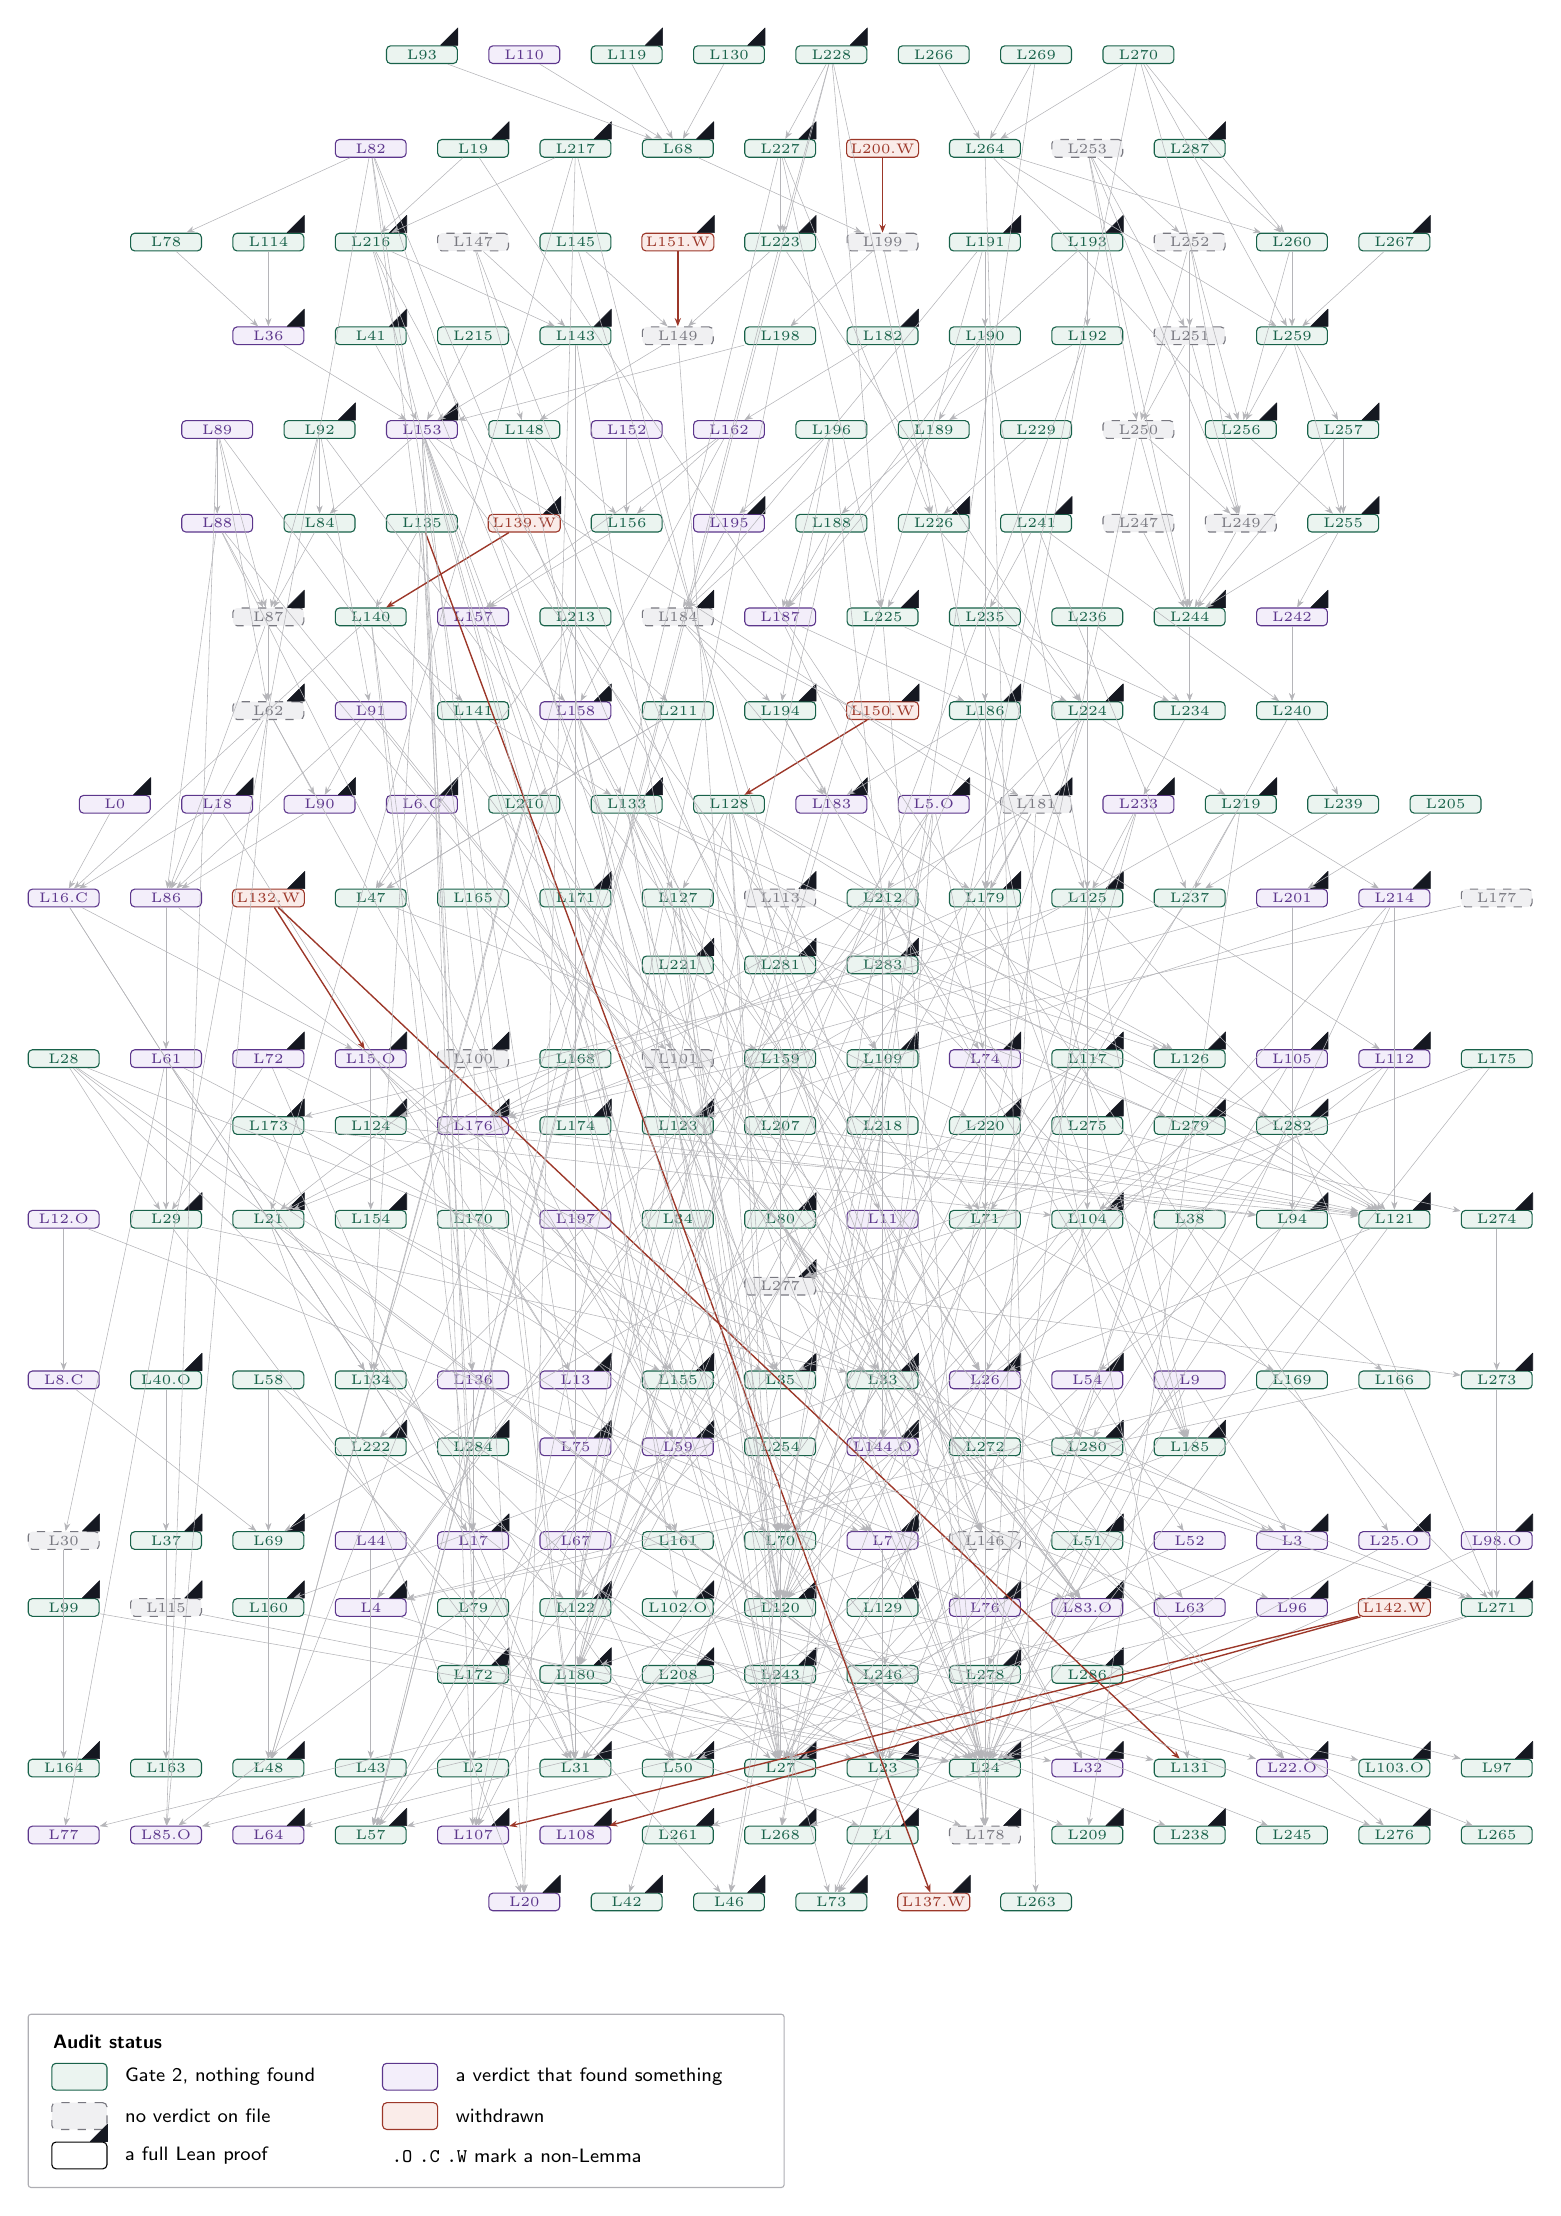
\begin{tikzpicture}[
  x=13mm,y=8.5mm,
  every node/.style={font=\tiny},
  res/.style={draw,rounded corners=1.5pt,inner sep=1.5pt,minimum width=9mm,align=center},
  ok/.style={res,draw=lemink,fill=lembg,text=lemink},
  gap/.style={res,draw=posedink,fill=posedbg,text=posedink},
  raw/.style={res,draw=openink,fill=openbg,text=openink,dashed},
  gone/.style={res,draw=deadink,fill=deadbg,text=deadink},
  halo/.style={res,draw=deadink,fill=deadbg,text=deadbg,inner xsep=9pt,inner ysep=7pt,minimum width=14mm,line width=.9pt},
  dep/.style={-{Stealth[length=3pt]},openink!55,line width=.2pt},
  bad/.style={-{Stealth[length=3pt]},deadink,line width=.5pt},
  lean/.style={fill=inkline,draw=inkline,line width=.2pt,line join=round},
]
\node[gap] (n0) at (-6.50,-11.20) {L0};
\node[ok] (n1) at (1.00,-26.60) {L1};
\node[ok] (n2) at (-3.00,-25.60) {L2};
\node[gap] (n3) at (5.00,-22.20) {L3};
\node[gap] (n4) at (-4.00,-23.20) {L4};
\node[gap] (n5) at (1.50,-11.20) {L5.O};
\node[gap] (n6) at (-3.50,-11.20) {L6.C};
\node[gap] (n7) at (1.00,-22.20) {L7};
\node[gap] (n8) at (-7.00,-19.80) {L8.C};
\node[gap] (n9) at (4.00,-19.80) {L9};
\node[gap] (n11) at (1.00,-17.40) {L11};
\node[gap] (n12) at (-7.00,-17.40) {L12.O};
\node[gap] (n13) at (-2.00,-19.80) {L13};
\node[gap] (n15) at (-4.00,-15.00) {L15.O};
\node[gap] (n16) at (-7.00,-12.60) {L16.C};
\node[gap] (n17) at (-3.00,-22.20) {L17};
\node[gap] (n18) at (-5.50,-11.20) {L18};
\node[ok] (n19) at (-3.00,-1.40) {L19};
\node[gap] (n20) at (-2.50,-27.60) {L20};
\node[ok] (n21) at (-5.00,-17.40) {L21};
\node[gap] (n22) at (5.00,-25.60) {L22.O};
\node[ok] (n23) at (1.00,-25.60) {L23};
\node[ok] (n24) at (2.00,-25.60) {L24};
\node[gap] (n25) at (6.00,-22.20) {L25.O};
\node[gap] (n26) at (2.00,-19.80) {L26};
\node[ok] (n27) at (0.00,-25.60) {L27};
\node[ok] (n28) at (-7.00,-15.00) {L28};
\node[ok] (n29) at (-6.00,-17.40) {L29};
\node[raw] (n30) at (-7.00,-22.20) {L30};
\node[ok] (n31) at (-2.00,-25.60) {L31};
\node[gap] (n32) at (3.00,-25.60) {L32};
\node[ok] (n33) at (1.00,-19.80) {L33};
\node[ok] (n34) at (-1.00,-17.40) {L34};
\node[ok] (n35) at (0.00,-19.80) {L35};
\node[gap] (n36) at (-5.00,-4.20) {L36};
\node[ok] (n37) at (-6.00,-22.20) {L37};
\node[ok] (n38) at (4.00,-17.40) {L38};
\node[ok] (n40) at (-6.00,-19.80) {L40.O};
\node[ok] (n41) at (-4.00,-4.20) {L41};
\node[ok] (n42) at (-1.50,-27.60) {L42};
\node[ok] (n43) at (-4.00,-25.60) {L43};
\node[gap] (n44) at (-4.00,-22.20) {L44};
\node[ok] (n46) at (-0.50,-27.60) {L46};
\node[ok] (n47) at (-4.00,-12.60) {L47};
\node[ok] (n48) at (-5.00,-25.60) {L48};
\node[ok] (n50) at (-1.00,-25.60) {L50};
\node[ok] (n51) at (3.00,-22.20) {L51};
\node[gap] (n52) at (4.00,-22.20) {L52};
\node[gap] (n54) at (3.00,-19.80) {L54};
\node[ok] (n57) at (-4.00,-26.60) {L57};
\node[ok] (n58) at (-5.00,-19.80) {L58};
\node[gap] (n59) at (-1.00,-20.80) {L59};
\node[gap] (n61) at (-6.00,-15.00) {L61};
\node[raw] (n62) at (-5.00,-9.80) {L62};
\node[gap] (n63) at (4.00,-23.20) {L63};
\node[gap] (n64) at (-5.00,-26.60) {L64};
\node[gap] (n67) at (-2.00,-22.20) {L67};
\node[ok] (n68) at (-1.00,-1.40) {L68};
\node[ok] (n69) at (-5.00,-22.20) {L69};
\node[ok] (n70) at (0.00,-22.20) {L70};
\node[ok] (n71) at (2.00,-17.40) {L71};
\node[gap] (n72) at (-5.00,-15.00) {L72};
\node[ok] (n73) at (0.50,-27.60) {L73};
\node[gap] (n74) at (2.00,-15.00) {L74};
\node[gap] (n75) at (-2.00,-20.80) {L75};
\node[gap] (n76) at (2.00,-23.20) {L76};
\node[gap] (n77) at (-7.00,-26.60) {L77};
\node[ok] (n78) at (-6.00,-2.80) {L78};
\node[ok] (n79) at (-3.00,-23.20) {L79};
\node[ok] (n80) at (0.00,-17.40) {L80};
\node[gap] (n82) at (-4.00,-1.40) {L82};
\node[gap] (n83) at (3.00,-23.20) {L83.O};
\node[ok] (n84) at (-4.50,-7.00) {L84};
\node[gap] (n85) at (-6.00,-26.60) {L85.O};
\node[gap] (n86) at (-6.00,-12.60) {L86};
\node[raw] (n87) at (-5.00,-8.40) {L87};
\node[gap] (n88) at (-5.50,-7.00) {L88};
\node[gap] (n89) at (-5.50,-5.60) {L89};
\node[gap] (n90) at (-4.50,-11.20) {L90};
\node[gap] (n91) at (-4.00,-9.80) {L91};
\node[ok] (n92) at (-4.50,-5.60) {L92};
\node[ok] (n93) at (-3.50,0.00) {L93};
\node[ok] (n94) at (5.00,-17.40) {L94};
\node[gap] (n96) at (5.00,-23.20) {L96};
\node[ok] (n97) at (7.00,-25.60) {L97};
\node[gap] (n98) at (7.00,-22.20) {L98.O};
\node[ok] (n99) at (-7.00,-23.20) {L99};
\node[raw] (n100) at (-3.00,-15.00) {L100};
\node[raw] (n101) at (-1.00,-15.00) {L101};
\node[ok] (n102) at (-1.00,-23.20) {L102.O};
\node[ok] (n103) at (6.00,-25.60) {L103.O};
\node[ok] (n104) at (3.00,-17.40) {L104};
\node[gap] (n105) at (5.00,-15.00) {L105};
\node[gap] (n107) at (-3.00,-26.60) {L107};
\node[gap] (n108) at (-2.00,-26.60) {L108};
\node[ok] (n109) at (1.00,-15.00) {L109};
\node[gap] (n110) at (-2.50,0.00) {L110};
\node[gap] (n112) at (6.00,-15.00) {L112};
\node[raw] (n113) at (0.00,-12.60) {L113};
\node[ok] (n114) at (-5.00,-2.80) {L114};
\node[raw] (n115) at (-6.00,-23.20) {L115};
\node[ok] (n117) at (3.00,-15.00) {L117};
\node[ok] (n119) at (-1.50,0.00) {L119};
\node[ok] (n120) at (0.00,-23.20) {L120};
\node[ok] (n121) at (6.00,-17.40) {L121};
\node[ok] (n122) at (-2.00,-23.20) {L122};
\node[ok] (n123) at (-1.00,-16.00) {L123};
\node[ok] (n124) at (-4.00,-16.00) {L124};
\node[ok] (n125) at (3.00,-12.60) {L125};
\node[ok] (n126) at (4.00,-15.00) {L126};
\node[ok] (n127) at (-1.00,-12.60) {L127};
\node[ok] (n128) at (-0.50,-11.20) {L128};
\node[ok] (n129) at (1.00,-23.20) {L129};
\node[ok] (n130) at (-0.50,0.00) {L130};
\node[ok] (n131) at (4.00,-25.60) {L131};
\node[gone] (n132) at (-5.00,-12.60) {L132.W};
\node[ok] (n133) at (-1.50,-11.20) {L133};
\node[ok] (n134) at (-4.00,-19.80) {L134};
\node[ok] (n135) at (-3.50,-7.00) {L135};
\node[gap] (n136) at (-3.00,-19.80) {L136};
\node[gone] (n137) at (1.50,-27.60) {L137.W};
\node[gone] (n139) at (-2.50,-7.00) {L139.W};
\node[ok] (n140) at (-4.00,-8.40) {L140};
\node[ok] (n141) at (-3.00,-9.80) {L141};
\node[gone] (n142) at (6.00,-23.20) {L142.W};
\node[ok] (n143) at (-2.00,-4.20) {L143};
\node[gap] (n144) at (1.00,-20.80) {L144.O};
\node[ok] (n145) at (-2.00,-2.80) {L145};
\node[raw] (n146) at (2.00,-22.20) {L146};
\node[raw] (n147) at (-3.00,-2.80) {L147};
\node[ok] (n148) at (-2.50,-5.60) {L148};
\node[raw] (n149) at (-1.00,-4.20) {L149};
\node[gone] (n150) at (1.00,-9.80) {L150.W};
\node[gone] (n151) at (-1.00,-2.80) {L151.W};
\node[gap] (n152) at (-1.50,-5.60) {L152};
\node[gap] (n153) at (-3.50,-5.60) {L153};
\node[ok] (n154) at (-4.00,-17.40) {L154};
\node[ok] (n155) at (-1.00,-19.80) {L155};
\node[ok] (n156) at (-1.50,-7.00) {L156};
\node[gap] (n157) at (-3.00,-8.40) {L157};
\node[gap] (n158) at (-2.00,-9.80) {L158};
\node[ok] (n159) at (0.00,-15.00) {L159};
\node[ok] (n160) at (-5.00,-23.20) {L160};
\node[ok] (n161) at (-1.00,-22.20) {L161};
\node[gap] (n162) at (-0.50,-5.60) {L162};
\node[ok] (n163) at (-6.00,-25.60) {L163};
\node[ok] (n164) at (-7.00,-25.60) {L164};
\node[ok] (n165) at (-3.00,-12.60) {L165};
\node[ok] (n166) at (6.00,-19.80) {L166};
\node[ok] (n168) at (-2.00,-15.00) {L168};
\node[ok] (n169) at (5.00,-19.80) {L169};
\node[ok] (n170) at (-3.00,-17.40) {L170};
\node[ok] (n171) at (-2.00,-12.60) {L171};
\node[ok] (n172) at (-3.00,-24.20) {L172};
\node[ok] (n173) at (-5.00,-16.00) {L173};
\node[ok] (n174) at (-2.00,-16.00) {L174};
\node[ok] (n175) at (7.00,-15.00) {L175};
\node[gap] (n176) at (-3.00,-16.00) {L176};
\node[raw] (n177) at (7.00,-12.60) {L177};
\node[raw] (n178) at (2.00,-26.60) {L178};
\node[ok] (n179) at (2.00,-12.60) {L179};
\node[ok] (n180) at (-2.00,-24.20) {L180};
\node[raw] (n181) at (2.50,-11.20) {L181};
\node[ok] (n182) at (1.00,-4.20) {L182};
\node[gap] (n183) at (0.50,-11.20) {L183};
\node[raw] (n184) at (-1.00,-8.40) {L184};
\node[ok] (n185) at (4.00,-20.80) {L185};
\node[ok] (n186) at (2.00,-9.80) {L186};
\node[gap] (n187) at (0.00,-8.40) {L187};
\node[ok] (n188) at (0.50,-7.00) {L188};
\node[ok] (n189) at (1.50,-5.60) {L189};
\node[ok] (n190) at (2.00,-4.20) {L190};
\node[ok] (n191) at (2.00,-2.80) {L191};
\node[ok] (n192) at (3.00,-4.20) {L192};
\node[ok] (n193) at (3.00,-2.80) {L193};
\node[ok] (n194) at (0.00,-9.80) {L194};
\node[gap] (n195) at (-0.50,-7.00) {L195};
\node[ok] (n196) at (0.50,-5.60) {L196};
\node[gap] (n197) at (-2.00,-17.40) {L197};
\node[ok] (n198) at (0.00,-4.20) {L198};
\node[raw] (n199) at (1.00,-2.80) {L199};
\node[gone] (n200) at (1.00,-1.40) {L200.W};
\node[gap] (n201) at (5.00,-12.60) {L201};
\node[ok] (n205) at (6.50,-11.20) {L205};
\node[ok] (n207) at (0.00,-16.00) {L207};
\node[ok] (n208) at (-1.00,-24.20) {L208};
\node[ok] (n209) at (3.00,-26.60) {L209};
\node[ok] (n210) at (-2.50,-11.20) {L210};
\node[ok] (n211) at (-1.00,-9.80) {L211};
\node[ok] (n212) at (1.00,-12.60) {L212};
\node[ok] (n213) at (-2.00,-8.40) {L213};
\node[gap] (n214) at (6.00,-12.60) {L214};
\node[ok] (n215) at (-3.00,-4.20) {L215};
\node[ok] (n216) at (-4.00,-2.80) {L216};
\node[ok] (n217) at (-2.00,-1.40) {L217};
\node[ok] (n218) at (1.00,-16.00) {L218};
\node[ok] (n219) at (4.50,-11.20) {L219};
\node[ok] (n220) at (2.00,-16.00) {L220};
\node[ok] (n221) at (-1.00,-13.60) {L221};
\node[ok] (n222) at (-4.00,-20.80) {L222};
\node[ok] (n223) at (0.00,-2.80) {L223};
\node[ok] (n224) at (3.00,-9.80) {L224};
\node[ok] (n225) at (1.00,-8.40) {L225};
\node[ok] (n226) at (1.50,-7.00) {L226};
\node[ok] (n227) at (0.00,-1.40) {L227};
\node[ok] (n228) at (0.50,0.00) {L228};
\node[ok] (n229) at (2.50,-5.60) {L229};
\node[gap] (n233) at (3.50,-11.20) {L233};
\node[ok] (n234) at (4.00,-9.80) {L234};
\node[ok] (n235) at (2.00,-8.40) {L235};
\node[ok] (n236) at (3.00,-8.40) {L236};
\node[ok] (n237) at (4.00,-12.60) {L237};
\node[ok] (n238) at (4.00,-26.60) {L238};
\node[ok] (n239) at (5.50,-11.20) {L239};
\node[ok] (n240) at (5.00,-9.80) {L240};
\node[ok] (n241) at (2.50,-7.00) {L241};
\node[gap] (n242) at (5.00,-8.40) {L242};
\node[ok] (n243) at (0.00,-24.20) {L243};
\node[ok] (n244) at (4.00,-8.40) {L244};
\node[ok] (n245) at (5.00,-26.60) {L245};
\node[ok] (n246) at (1.00,-24.20) {L246};
\node[raw] (n247) at (3.50,-7.00) {L247};
\node[raw] (n249) at (4.50,-7.00) {L249};
\node[raw] (n250) at (3.50,-5.60) {L250};
\node[raw] (n251) at (4.00,-4.20) {L251};
\node[raw] (n252) at (4.00,-2.80) {L252};
\node[raw] (n253) at (3.00,-1.40) {L253};
\node[ok] (n254) at (0.00,-20.80) {L254};
\node[ok] (n255) at (5.50,-7.00) {L255};
\node[ok] (n256) at (4.50,-5.60) {L256};
\node[ok] (n257) at (5.50,-5.60) {L257};
\node[ok] (n259) at (5.00,-4.20) {L259};
\node[ok] (n260) at (5.00,-2.80) {L260};
\node[ok] (n261) at (-1.00,-26.60) {L261};
\node[ok] (n263) at (2.50,-27.60) {L263};
\node[ok] (n264) at (2.00,-1.40) {L264};
\node[ok] (n265) at (7.00,-26.60) {L265};
\node[ok] (n266) at (1.50,0.00) {L266};
\node[ok] (n267) at (6.00,-2.80) {L267};
\node[ok] (n268) at (0.00,-26.60) {L268};
\node[ok] (n269) at (2.50,0.00) {L269};
\node[ok] (n270) at (3.50,0.00) {L270};
\node[ok] (n271) at (7.00,-23.20) {L271};
\node[ok] (n272) at (2.00,-20.80) {L272};
\node[ok] (n273) at (7.00,-19.80) {L273};
\node[ok] (n274) at (7.00,-17.40) {L274};
\node[ok] (n275) at (3.00,-16.00) {L275};
\node[ok] (n276) at (6.00,-26.60) {L276};
\node[raw] (n277) at (0.00,-18.40) {L277};
\node[ok] (n278) at (2.00,-24.20) {L278};
\node[ok] (n279) at (4.00,-16.00) {L279};
\node[ok] (n280) at (3.00,-20.80) {L280};
\node[ok] (n281) at (0.00,-13.60) {L281};
\node[ok] (n282) at (5.00,-16.00) {L282};
\node[ok] (n283) at (1.00,-13.60) {L283};
\node[ok] (n284) at (-3.00,-20.80) {L284};
\node[ok] (n286) at (3.00,-24.20) {L286};
\node[ok] (n287) at (4.00,-1.40) {L287};
\fill[lean] (n0.north east) -- ++(-2.2mm,0) -- ++(2.2mm,2.2mm) -- cycle;
\fill[lean] (n1.north east) -- ++(-2.2mm,0) -- ++(2.2mm,2.2mm) -- cycle;
\fill[lean] (n3.north east) -- ++(-2.2mm,0) -- ++(2.2mm,2.2mm) -- cycle;
\fill[lean] (n4.north east) -- ++(-2.2mm,0) -- ++(2.2mm,2.2mm) -- cycle;
\fill[lean] (n5.north east) -- ++(-2.2mm,0) -- ++(2.2mm,2.2mm) -- cycle;
\fill[lean] (n6.north east) -- ++(-2.2mm,0) -- ++(2.2mm,2.2mm) -- cycle;
\fill[lean] (n7.north east) -- ++(-2.2mm,0) -- ++(2.2mm,2.2mm) -- cycle;
\fill[lean] (n13.north east) -- ++(-2.2mm,0) -- ++(2.2mm,2.2mm) -- cycle;
\fill[lean] (n15.north east) -- ++(-2.2mm,0) -- ++(2.2mm,2.2mm) -- cycle;
\fill[lean] (n17.north east) -- ++(-2.2mm,0) -- ++(2.2mm,2.2mm) -- cycle;
\fill[lean] (n18.north east) -- ++(-2.2mm,0) -- ++(2.2mm,2.2mm) -- cycle;
\fill[lean] (n19.north east) -- ++(-2.2mm,0) -- ++(2.2mm,2.2mm) -- cycle;
\fill[lean] (n20.north east) -- ++(-2.2mm,0) -- ++(2.2mm,2.2mm) -- cycle;
\fill[lean] (n21.north east) -- ++(-2.2mm,0) -- ++(2.2mm,2.2mm) -- cycle;
\fill[lean] (n22.north east) -- ++(-2.2mm,0) -- ++(2.2mm,2.2mm) -- cycle;
\fill[lean] (n23.north east) -- ++(-2.2mm,0) -- ++(2.2mm,2.2mm) -- cycle;
\fill[lean] (n24.north east) -- ++(-2.2mm,0) -- ++(2.2mm,2.2mm) -- cycle;
\fill[lean] (n25.north east) -- ++(-2.2mm,0) -- ++(2.2mm,2.2mm) -- cycle;
\fill[lean] (n26.north east) -- ++(-2.2mm,0) -- ++(2.2mm,2.2mm) -- cycle;
\fill[lean] (n27.north east) -- ++(-2.2mm,0) -- ++(2.2mm,2.2mm) -- cycle;
\fill[lean] (n29.north east) -- ++(-2.2mm,0) -- ++(2.2mm,2.2mm) -- cycle;
\fill[lean] (n30.north east) -- ++(-2.2mm,0) -- ++(2.2mm,2.2mm) -- cycle;
\fill[lean] (n31.north east) -- ++(-2.2mm,0) -- ++(2.2mm,2.2mm) -- cycle;
\fill[lean] (n32.north east) -- ++(-2.2mm,0) -- ++(2.2mm,2.2mm) -- cycle;
\fill[lean] (n33.north east) -- ++(-2.2mm,0) -- ++(2.2mm,2.2mm) -- cycle;
\fill[lean] (n35.north east) -- ++(-2.2mm,0) -- ++(2.2mm,2.2mm) -- cycle;
\fill[lean] (n36.north east) -- ++(-2.2mm,0) -- ++(2.2mm,2.2mm) -- cycle;
\fill[lean] (n37.north east) -- ++(-2.2mm,0) -- ++(2.2mm,2.2mm) -- cycle;
\fill[lean] (n40.north east) -- ++(-2.2mm,0) -- ++(2.2mm,2.2mm) -- cycle;
\fill[lean] (n41.north east) -- ++(-2.2mm,0) -- ++(2.2mm,2.2mm) -- cycle;
\fill[lean] (n42.north east) -- ++(-2.2mm,0) -- ++(2.2mm,2.2mm) -- cycle;
\fill[lean] (n46.north east) -- ++(-2.2mm,0) -- ++(2.2mm,2.2mm) -- cycle;
\fill[lean] (n48.north east) -- ++(-2.2mm,0) -- ++(2.2mm,2.2mm) -- cycle;
\fill[lean] (n50.north east) -- ++(-2.2mm,0) -- ++(2.2mm,2.2mm) -- cycle;
\fill[lean] (n51.north east) -- ++(-2.2mm,0) -- ++(2.2mm,2.2mm) -- cycle;
\fill[lean] (n54.north east) -- ++(-2.2mm,0) -- ++(2.2mm,2.2mm) -- cycle;
\fill[lean] (n57.north east) -- ++(-2.2mm,0) -- ++(2.2mm,2.2mm) -- cycle;
\fill[lean] (n59.north east) -- ++(-2.2mm,0) -- ++(2.2mm,2.2mm) -- cycle;
\fill[lean] (n62.north east) -- ++(-2.2mm,0) -- ++(2.2mm,2.2mm) -- cycle;
\fill[lean] (n64.north east) -- ++(-2.2mm,0) -- ++(2.2mm,2.2mm) -- cycle;
\fill[lean] (n68.north east) -- ++(-2.2mm,0) -- ++(2.2mm,2.2mm) -- cycle;
\fill[lean] (n69.north east) -- ++(-2.2mm,0) -- ++(2.2mm,2.2mm) -- cycle;
\fill[lean] (n72.north east) -- ++(-2.2mm,0) -- ++(2.2mm,2.2mm) -- cycle;
\fill[lean] (n73.north east) -- ++(-2.2mm,0) -- ++(2.2mm,2.2mm) -- cycle;
\fill[lean] (n74.north east) -- ++(-2.2mm,0) -- ++(2.2mm,2.2mm) -- cycle;
\fill[lean] (n75.north east) -- ++(-2.2mm,0) -- ++(2.2mm,2.2mm) -- cycle;
\fill[lean] (n76.north east) -- ++(-2.2mm,0) -- ++(2.2mm,2.2mm) -- cycle;
\fill[lean] (n80.north east) -- ++(-2.2mm,0) -- ++(2.2mm,2.2mm) -- cycle;
\fill[lean] (n83.north east) -- ++(-2.2mm,0) -- ++(2.2mm,2.2mm) -- cycle;
\fill[lean] (n87.north east) -- ++(-2.2mm,0) -- ++(2.2mm,2.2mm) -- cycle;
\fill[lean] (n90.north east) -- ++(-2.2mm,0) -- ++(2.2mm,2.2mm) -- cycle;
\fill[lean] (n92.north east) -- ++(-2.2mm,0) -- ++(2.2mm,2.2mm) -- cycle;
\fill[lean] (n93.north east) -- ++(-2.2mm,0) -- ++(2.2mm,2.2mm) -- cycle;
\fill[lean] (n94.north east) -- ++(-2.2mm,0) -- ++(2.2mm,2.2mm) -- cycle;
\fill[lean] (n96.north east) -- ++(-2.2mm,0) -- ++(2.2mm,2.2mm) -- cycle;
\fill[lean] (n97.north east) -- ++(-2.2mm,0) -- ++(2.2mm,2.2mm) -- cycle;
\fill[lean] (n98.north east) -- ++(-2.2mm,0) -- ++(2.2mm,2.2mm) -- cycle;
\fill[lean] (n99.north east) -- ++(-2.2mm,0) -- ++(2.2mm,2.2mm) -- cycle;
\fill[lean] (n100.north east) -- ++(-2.2mm,0) -- ++(2.2mm,2.2mm) -- cycle;
\fill[lean] (n102.north east) -- ++(-2.2mm,0) -- ++(2.2mm,2.2mm) -- cycle;
\fill[lean] (n103.north east) -- ++(-2.2mm,0) -- ++(2.2mm,2.2mm) -- cycle;
\fill[lean] (n104.north east) -- ++(-2.2mm,0) -- ++(2.2mm,2.2mm) -- cycle;
\fill[lean] (n105.north east) -- ++(-2.2mm,0) -- ++(2.2mm,2.2mm) -- cycle;
\fill[lean] (n107.north east) -- ++(-2.2mm,0) -- ++(2.2mm,2.2mm) -- cycle;
\fill[lean] (n108.north east) -- ++(-2.2mm,0) -- ++(2.2mm,2.2mm) -- cycle;
\fill[lean] (n109.north east) -- ++(-2.2mm,0) -- ++(2.2mm,2.2mm) -- cycle;
\fill[lean] (n112.north east) -- ++(-2.2mm,0) -- ++(2.2mm,2.2mm) -- cycle;
\fill[lean] (n113.north east) -- ++(-2.2mm,0) -- ++(2.2mm,2.2mm) -- cycle;
\fill[lean] (n114.north east) -- ++(-2.2mm,0) -- ++(2.2mm,2.2mm) -- cycle;
\fill[lean] (n115.north east) -- ++(-2.2mm,0) -- ++(2.2mm,2.2mm) -- cycle;
\fill[lean] (n117.north east) -- ++(-2.2mm,0) -- ++(2.2mm,2.2mm) -- cycle;
\fill[lean] (n119.north east) -- ++(-2.2mm,0) -- ++(2.2mm,2.2mm) -- cycle;
\fill[lean] (n120.north east) -- ++(-2.2mm,0) -- ++(2.2mm,2.2mm) -- cycle;
\fill[lean] (n121.north east) -- ++(-2.2mm,0) -- ++(2.2mm,2.2mm) -- cycle;
\fill[lean] (n122.north east) -- ++(-2.2mm,0) -- ++(2.2mm,2.2mm) -- cycle;
\fill[lean] (n123.north east) -- ++(-2.2mm,0) -- ++(2.2mm,2.2mm) -- cycle;
\fill[lean] (n124.north east) -- ++(-2.2mm,0) -- ++(2.2mm,2.2mm) -- cycle;
\fill[lean] (n125.north east) -- ++(-2.2mm,0) -- ++(2.2mm,2.2mm) -- cycle;
\fill[lean] (n126.north east) -- ++(-2.2mm,0) -- ++(2.2mm,2.2mm) -- cycle;
\fill[lean] (n129.north east) -- ++(-2.2mm,0) -- ++(2.2mm,2.2mm) -- cycle;
\fill[lean] (n130.north east) -- ++(-2.2mm,0) -- ++(2.2mm,2.2mm) -- cycle;
\fill[lean] (n132.north east) -- ++(-2.2mm,0) -- ++(2.2mm,2.2mm) -- cycle;
\fill[lean] (n133.north east) -- ++(-2.2mm,0) -- ++(2.2mm,2.2mm) -- cycle;
\fill[lean] (n137.north east) -- ++(-2.2mm,0) -- ++(2.2mm,2.2mm) -- cycle;
\fill[lean] (n139.north east) -- ++(-2.2mm,0) -- ++(2.2mm,2.2mm) -- cycle;
\fill[lean] (n142.north east) -- ++(-2.2mm,0) -- ++(2.2mm,2.2mm) -- cycle;
\fill[lean] (n143.north east) -- ++(-2.2mm,0) -- ++(2.2mm,2.2mm) -- cycle;
\fill[lean] (n144.north east) -- ++(-2.2mm,0) -- ++(2.2mm,2.2mm) -- cycle;
\fill[lean] (n150.north east) -- ++(-2.2mm,0) -- ++(2.2mm,2.2mm) -- cycle;
\fill[lean] (n151.north east) -- ++(-2.2mm,0) -- ++(2.2mm,2.2mm) -- cycle;
\fill[lean] (n153.north east) -- ++(-2.2mm,0) -- ++(2.2mm,2.2mm) -- cycle;
\fill[lean] (n154.north east) -- ++(-2.2mm,0) -- ++(2.2mm,2.2mm) -- cycle;
\fill[lean] (n155.north east) -- ++(-2.2mm,0) -- ++(2.2mm,2.2mm) -- cycle;
\fill[lean] (n158.north east) -- ++(-2.2mm,0) -- ++(2.2mm,2.2mm) -- cycle;
\fill[lean] (n160.north east) -- ++(-2.2mm,0) -- ++(2.2mm,2.2mm) -- cycle;
\fill[lean] (n164.north east) -- ++(-2.2mm,0) -- ++(2.2mm,2.2mm) -- cycle;
\fill[lean] (n171.north east) -- ++(-2.2mm,0) -- ++(2.2mm,2.2mm) -- cycle;
\fill[lean] (n172.north east) -- ++(-2.2mm,0) -- ++(2.2mm,2.2mm) -- cycle;
\fill[lean] (n173.north east) -- ++(-2.2mm,0) -- ++(2.2mm,2.2mm) -- cycle;
\fill[lean] (n174.north east) -- ++(-2.2mm,0) -- ++(2.2mm,2.2mm) -- cycle;
\fill[lean] (n176.north east) -- ++(-2.2mm,0) -- ++(2.2mm,2.2mm) -- cycle;
\fill[lean] (n178.north east) -- ++(-2.2mm,0) -- ++(2.2mm,2.2mm) -- cycle;
\fill[lean] (n179.north east) -- ++(-2.2mm,0) -- ++(2.2mm,2.2mm) -- cycle;
\fill[lean] (n180.north east) -- ++(-2.2mm,0) -- ++(2.2mm,2.2mm) -- cycle;
\fill[lean] (n181.north east) -- ++(-2.2mm,0) -- ++(2.2mm,2.2mm) -- cycle;
\fill[lean] (n182.north east) -- ++(-2.2mm,0) -- ++(2.2mm,2.2mm) -- cycle;
\fill[lean] (n183.north east) -- ++(-2.2mm,0) -- ++(2.2mm,2.2mm) -- cycle;
\fill[lean] (n184.north east) -- ++(-2.2mm,0) -- ++(2.2mm,2.2mm) -- cycle;
\fill[lean] (n185.north east) -- ++(-2.2mm,0) -- ++(2.2mm,2.2mm) -- cycle;
\fill[lean] (n186.north east) -- ++(-2.2mm,0) -- ++(2.2mm,2.2mm) -- cycle;
\fill[lean] (n191.north east) -- ++(-2.2mm,0) -- ++(2.2mm,2.2mm) -- cycle;
\fill[lean] (n193.north east) -- ++(-2.2mm,0) -- ++(2.2mm,2.2mm) -- cycle;
\fill[lean] (n194.north east) -- ++(-2.2mm,0) -- ++(2.2mm,2.2mm) -- cycle;
\fill[lean] (n195.north east) -- ++(-2.2mm,0) -- ++(2.2mm,2.2mm) -- cycle;
\fill[lean] (n201.north east) -- ++(-2.2mm,0) -- ++(2.2mm,2.2mm) -- cycle;
\fill[lean] (n208.north east) -- ++(-2.2mm,0) -- ++(2.2mm,2.2mm) -- cycle;
\fill[lean] (n209.north east) -- ++(-2.2mm,0) -- ++(2.2mm,2.2mm) -- cycle;
\fill[lean] (n214.north east) -- ++(-2.2mm,0) -- ++(2.2mm,2.2mm) -- cycle;
\fill[lean] (n216.north east) -- ++(-2.2mm,0) -- ++(2.2mm,2.2mm) -- cycle;
\fill[lean] (n217.north east) -- ++(-2.2mm,0) -- ++(2.2mm,2.2mm) -- cycle;
\fill[lean] (n219.north east) -- ++(-2.2mm,0) -- ++(2.2mm,2.2mm) -- cycle;
\fill[lean] (n220.north east) -- ++(-2.2mm,0) -- ++(2.2mm,2.2mm) -- cycle;
\fill[lean] (n221.north east) -- ++(-2.2mm,0) -- ++(2.2mm,2.2mm) -- cycle;
\fill[lean] (n222.north east) -- ++(-2.2mm,0) -- ++(2.2mm,2.2mm) -- cycle;
\fill[lean] (n223.north east) -- ++(-2.2mm,0) -- ++(2.2mm,2.2mm) -- cycle;
\fill[lean] (n224.north east) -- ++(-2.2mm,0) -- ++(2.2mm,2.2mm) -- cycle;
\fill[lean] (n225.north east) -- ++(-2.2mm,0) -- ++(2.2mm,2.2mm) -- cycle;
\fill[lean] (n226.north east) -- ++(-2.2mm,0) -- ++(2.2mm,2.2mm) -- cycle;
\fill[lean] (n227.north east) -- ++(-2.2mm,0) -- ++(2.2mm,2.2mm) -- cycle;
\fill[lean] (n228.north east) -- ++(-2.2mm,0) -- ++(2.2mm,2.2mm) -- cycle;
\fill[lean] (n233.north east) -- ++(-2.2mm,0) -- ++(2.2mm,2.2mm) -- cycle;
\fill[lean] (n238.north east) -- ++(-2.2mm,0) -- ++(2.2mm,2.2mm) -- cycle;
\fill[lean] (n241.north east) -- ++(-2.2mm,0) -- ++(2.2mm,2.2mm) -- cycle;
\fill[lean] (n242.north east) -- ++(-2.2mm,0) -- ++(2.2mm,2.2mm) -- cycle;
\fill[lean] (n243.north east) -- ++(-2.2mm,0) -- ++(2.2mm,2.2mm) -- cycle;
\fill[lean] (n244.north east) -- ++(-2.2mm,0) -- ++(2.2mm,2.2mm) -- cycle;
\fill[lean] (n255.north east) -- ++(-2.2mm,0) -- ++(2.2mm,2.2mm) -- cycle;
\fill[lean] (n256.north east) -- ++(-2.2mm,0) -- ++(2.2mm,2.2mm) -- cycle;
\fill[lean] (n257.north east) -- ++(-2.2mm,0) -- ++(2.2mm,2.2mm) -- cycle;
\fill[lean] (n259.north east) -- ++(-2.2mm,0) -- ++(2.2mm,2.2mm) -- cycle;
\fill[lean] (n261.north east) -- ++(-2.2mm,0) -- ++(2.2mm,2.2mm) -- cycle;
\fill[lean] (n267.north east) -- ++(-2.2mm,0) -- ++(2.2mm,2.2mm) -- cycle;
\fill[lean] (n268.north east) -- ++(-2.2mm,0) -- ++(2.2mm,2.2mm) -- cycle;
\fill[lean] (n271.north east) -- ++(-2.2mm,0) -- ++(2.2mm,2.2mm) -- cycle;
\fill[lean] (n273.north east) -- ++(-2.2mm,0) -- ++(2.2mm,2.2mm) -- cycle;
\fill[lean] (n274.north east) -- ++(-2.2mm,0) -- ++(2.2mm,2.2mm) -- cycle;
\fill[lean] (n275.north east) -- ++(-2.2mm,0) -- ++(2.2mm,2.2mm) -- cycle;
\fill[lean] (n276.north east) -- ++(-2.2mm,0) -- ++(2.2mm,2.2mm) -- cycle;
\fill[lean] (n277.north east) -- ++(-2.2mm,0) -- ++(2.2mm,2.2mm) -- cycle;
\fill[lean] (n278.north east) -- ++(-2.2mm,0) -- ++(2.2mm,2.2mm) -- cycle;
\fill[lean] (n279.north east) -- ++(-2.2mm,0) -- ++(2.2mm,2.2mm) -- cycle;
\fill[lean] (n280.north east) -- ++(-2.2mm,0) -- ++(2.2mm,2.2mm) -- cycle;
\fill[lean] (n281.north east) -- ++(-2.2mm,0) -- ++(2.2mm,2.2mm) -- cycle;
\fill[lean] (n282.north east) -- ++(-2.2mm,0) -- ++(2.2mm,2.2mm) -- cycle;
\fill[lean] (n283.north east) -- ++(-2.2mm,0) -- ++(2.2mm,2.2mm) -- cycle;
\fill[lean] (n284.north east) -- ++(-2.2mm,0) -- ++(2.2mm,2.2mm) -- cycle;
\fill[lean] (n286.north east) -- ++(-2.2mm,0) -- ++(2.2mm,2.2mm) -- cycle;
\fill[lean] (n287.north east) -- ++(-2.2mm,0) -- ++(2.2mm,2.2mm) -- cycle;
\draw[dep] (n0) -- (n16);
\draw[dep] (n3) -- (n24);
\draw[dep] (n3) -- (n27);
\draw[dep] (n4) -- (n23);
\draw[dep] (n5) -- (n4);
\draw[dep] (n5) -- (n46);
\draw[dep] (n5) -- (n74);
\draw[dep] (n5) -- (n144);
\draw[dep] (n5) -- (n212);
\draw[dep] (n6) -- (n47);
\draw[dep] (n7) -- (n23);
\draw[dep] (n8) -- (n69);
\draw[dep] (n9) -- (n3);
\draw[dep] (n9) -- (n24);
\draw[dep] (n9) -- (n27);
\draw[dep] (n11) -- (n24);
\draw[dep] (n11) -- (n26);
\draw[dep] (n12) -- (n7);
\draw[dep] (n12) -- (n8);
\draw[dep] (n13) -- (n161);
\draw[dep] (n15) -- (n7);
\draw[dep] (n15) -- (n154);
\draw[dep] (n15) -- (n155);
\draw[dep] (n16) -- (n15);
\draw[dep] (n16) -- (n17);
\draw[dep] (n16) -- (n134);
\draw[dep] (n17) -- (n2);
\draw[dep] (n18) -- (n13);
\draw[dep] (n18) -- (n16);
\draw[dep] (n19) -- (n25);
\draw[dep] (n19) -- (n216);
\draw[dep] (n21) -- (n20);
\draw[dep] (n21) -- (n24);
\draw[dep] (n21) -- (n134);
\draw[dep] (n25) -- (n24);
\draw[dep] (n26) -- (n3);
\draw[dep] (n26) -- (n24);
\draw[dep] (n26) -- (n27);
\draw[dep] (n28) -- (n3);
\draw[dep] (n28) -- (n24);
\draw[dep] (n28) -- (n27);
\draw[dep] (n28) -- (n29);
\draw[dep] (n28) -- (n70);
\draw[dep] (n29) -- (n31);
\draw[dep] (n29) -- (n33);
\draw[dep] (n30) -- (n164);
\draw[dep] (n33) -- (n32);
\draw[dep] (n33) -- (n160);
\draw[dep] (n34) -- (n35);
\draw[dep] (n35) -- (n42);
\draw[dep] (n35) -- (n70);
\draw[dep] (n36) -- (n153);
\draw[dep] (n37) -- (n163);
\draw[dep] (n38) -- (n166);
\draw[dep] (n40) -- (n37);
\draw[dep] (n41) -- (n153);
\draw[dep] (n44) -- (n43);
\draw[dep] (n47) -- (n159);
\draw[dep] (n51) -- (n24);
\draw[dep] (n51) -- (n27);
\draw[dep] (n52) -- (n50);
\draw[dep] (n54) -- (n50);
\draw[dep] (n54) -- (n52);
\draw[dep] (n58) -- (n23);
\draw[dep] (n58) -- (n46);
\draw[dep] (n58) -- (n69);
\draw[dep] (n59) -- (n83);
\draw[dep] (n59) -- (n85);
\draw[dep] (n61) -- (n29);
\draw[dep] (n61) -- (n30);
\draw[dep] (n61) -- (n35);
\draw[dep] (n61) -- (n50);
\draw[dep] (n62) -- (n59);
\draw[dep] (n62) -- (n85);
\draw[dep] (n62) -- (n86);
\draw[dep] (n62) -- (n90);
\draw[dep] (n63) -- (n64);
\draw[dep] (n67) -- (n50);
\draw[dep] (n68) -- (n199);
\draw[dep] (n69) -- (n48);
\draw[dep] (n70) -- (n23);
\draw[dep] (n70) -- (n31);
\draw[dep] (n71) -- (n70);
\draw[dep] (n71) -- (n169);
\draw[dep] (n72) -- (n29);
\draw[dep] (n72) -- (n31);
\draw[dep] (n72) -- (n33);
\draw[dep] (n74) -- (n70);
\draw[dep] (n74) -- (n71);
\draw[dep] (n75) -- (n76);
\draw[dep] (n76) -- (n77);
\draw[dep] (n78) -- (n36);
\draw[dep] (n79) -- (n131);
\draw[dep] (n80) -- (n32);
\draw[dep] (n80) -- (n33);
\draw[dep] (n82) -- (n31);
\draw[dep] (n82) -- (n33);
\draw[dep] (n82) -- (n35);
\draw[dep] (n82) -- (n75);
\draw[dep] (n82) -- (n77);
\draw[dep] (n82) -- (n78);
\draw[dep] (n83) -- (n85);
\draw[dep] (n84) -- (n83);
\draw[dep] (n84) -- (n87);
\draw[dep] (n86) -- (n61);
\draw[dep] (n86) -- (n83);
\draw[dep] (n87) -- (n62);
\draw[dep] (n87) -- (n83);
\draw[dep] (n87) -- (n86);
\draw[dep] (n88) -- (n59);
\draw[dep] (n88) -- (n83);
\draw[dep] (n88) -- (n86);
\draw[dep] (n88) -- (n87);
\draw[dep] (n89) -- (n62);
\draw[dep] (n89) -- (n83);
\draw[dep] (n89) -- (n85);
\draw[dep] (n89) -- (n87);
\draw[dep] (n89) -- (n88);
\draw[dep] (n90) -- (n86);
\draw[dep] (n91) -- (n83);
\draw[dep] (n91) -- (n86);
\draw[dep] (n91) -- (n90);
\draw[dep] (n92) -- (n63);
\draw[dep] (n92) -- (n84);
\draw[dep] (n92) -- (n87);
\draw[dep] (n92) -- (n91);
\draw[dep] (n93) -- (n68);
\draw[dep] (n94) -- (n54);
\draw[dep] (n96) -- (n57);
\draw[dep] (n98) -- (n24);
\draw[dep] (n99) -- (n24);
\draw[dep] (n100) -- (n20);
\draw[dep] (n100) -- (n21);
\draw[dep] (n101) -- (n21);
\draw[dep] (n102) -- (n22);
\draw[dep] (n102) -- (n103);
\draw[dep] (n104) -- (n31);
\draw[dep] (n104) -- (n35);
\draw[dep] (n104) -- (n73);
\draw[dep] (n105) -- (n23);
\draw[dep] (n105) -- (n104);
\draw[dep] (n109) -- (n70);
\draw[dep] (n109) -- (n71);
\draw[dep] (n109) -- (n107);
\draw[dep] (n110) -- (n68);
\draw[dep] (n112) -- (n70);
\draw[dep] (n112) -- (n73);
\draw[dep] (n112) -- (n104);
\draw[dep] (n113) -- (n107);
\draw[dep] (n113) -- (n109);
\draw[dep] (n114) -- (n36);
\draw[dep] (n115) -- (n24);
\draw[dep] (n117) -- (n69);
\draw[dep] (n117) -- (n70);
\draw[dep] (n117) -- (n71);
\draw[dep] (n119) -- (n68);
\draw[dep] (n120) -- (n24);
\draw[dep] (n121) -- (n24);
\draw[dep] (n121) -- (n26);
\draw[dep] (n122) -- (n24);
\draw[dep] (n123) -- (n24);
\draw[dep] (n123) -- (n120);
\draw[dep] (n123) -- (n121);
\draw[dep] (n123) -- (n122);
\draw[dep] (n124) -- (n24);
\draw[dep] (n124) -- (n121);
\draw[dep] (n125) -- (n24);
\draw[dep] (n125) -- (n121);
\draw[dep] (n125) -- (n124);
\draw[dep] (n126) -- (n24);
\draw[dep] (n126) -- (n27);
\draw[dep] (n126) -- (n120);
\draw[dep] (n126) -- (n121);
\draw[dep] (n127) -- (n24);
\draw[dep] (n127) -- (n27);
\draw[dep] (n127) -- (n120);
\draw[dep] (n127) -- (n121);
\draw[dep] (n127) -- (n122);
\draw[dep] (n127) -- (n126);
\draw[dep] (n128) -- (n11);
\draw[dep] (n128) -- (n24);
\draw[dep] (n128) -- (n27);
\draw[dep] (n128) -- (n120);
\draw[dep] (n128) -- (n121);
\draw[dep] (n128) -- (n122);
\draw[dep] (n128) -- (n126);
\draw[dep] (n128) -- (n127);
\draw[dep] (n129) -- (n97);
\draw[dep] (n130) -- (n68);
\draw[bad] (n132) -- (n15);
\draw[bad] (n132) -- (n131);
\draw[dep] (n133) -- (n24);
\draw[dep] (n133) -- (n26);
\draw[dep] (n133) -- (n27);
\draw[dep] (n133) -- (n120);
\draw[dep] (n133) -- (n121);
\draw[dep] (n133) -- (n126);
\draw[dep] (n133) -- (n127);
\draw[dep] (n134) -- (n17);
\draw[dep] (n134) -- (n24);
\draw[dep] (n135) -- (n17);
\draw[dep] (n135) -- (n134);
\draw[dep] (n135) -- (n136);
\draw[bad] (n135) -- (n137);
\draw[dep] (n135) -- (n140);
\draw[dep] (n136) -- (n17);
\draw[bad] (n139) -- (n140);
\draw[dep] (n140) -- (n16);
\draw[dep] (n140) -- (n17);
\draw[dep] (n140) -- (n136);
\draw[dep] (n140) -- (n141);
\draw[dep] (n141) -- (n27);
\draw[dep] (n141) -- (n120);
\draw[dep] (n141) -- (n133);
\draw[bad] (n142) -- (n107);
\draw[bad] (n142) -- (n108);
\draw[dep] (n143) -- (n31);
\draw[dep] (n143) -- (n70);
\draw[dep] (n143) -- (n153);
\draw[dep] (n144) -- (n96);
\draw[dep] (n145) -- (n146);
\draw[dep] (n145) -- (n149);
\draw[dep] (n146) -- (n27);
\draw[dep] (n147) -- (n143);
\draw[dep] (n147) -- (n146);
\draw[dep] (n147) -- (n148);
\draw[dep] (n148) -- (n27);
\draw[dep] (n148) -- (n146);
\draw[dep] (n148) -- (n156);
\draw[dep] (n149) -- (n27);
\draw[dep] (n149) -- (n148);
\draw[bad] (n150) -- (n128);
\draw[bad] (n151) -- (n149);
\draw[dep] (n152) -- (n156);
\draw[dep] (n153) -- (n23);
\draw[dep] (n153) -- (n31);
\draw[dep] (n153) -- (n35);
\draw[dep] (n153) -- (n70);
\draw[dep] (n153) -- (n73);
\draw[dep] (n153) -- (n79);
\draw[dep] (n153) -- (n84);
\draw[dep] (n153) -- (n107);
\draw[dep] (n153) -- (n109);
\draw[dep] (n153) -- (n112);
\draw[dep] (n154) -- (n7);
\draw[dep] (n154) -- (n155);
\draw[dep] (n155) -- (n7);
\draw[dep] (n156) -- (n157);
\draw[dep] (n157) -- (n158);
\draw[dep] (n158) -- (n70);
\draw[dep] (n158) -- (n133);
\draw[dep] (n158) -- (n134);
\draw[dep] (n158) -- (n146);
\draw[dep] (n159) -- (n27);
\draw[dep] (n159) -- (n71);
\draw[dep] (n160) -- (n32);
\draw[dep] (n161) -- (n27);
\draw[dep] (n162) -- (n156);
\draw[dep] (n162) -- (n157);
\draw[dep] (n162) -- (n158);
\draw[dep] (n165) -- (n22);
\draw[dep] (n165) -- (n101);
\draw[dep] (n166) -- (n4);
\draw[dep] (n168) -- (n21);
\draw[dep] (n168) -- (n161);
\draw[dep] (n169) -- (n4);
\draw[dep] (n170) -- (n13);
\draw[dep] (n171) -- (n22);
\draw[dep] (n171) -- (n101);
\draw[dep] (n171) -- (n102);
\draw[dep] (n172) -- (n1);
\draw[dep] (n173) -- (n31);
\draw[dep] (n173) -- (n104);
\draw[dep] (n174) -- (n94);
\draw[dep] (n175) -- (n73);
\draw[dep] (n175) -- (n104);
\draw[dep] (n176) -- (n24);
\draw[dep] (n176) -- (n94);
\draw[dep] (n177) -- (n176);
\draw[dep] (n179) -- (n176);
\draw[dep] (n179) -- (n178);
\draw[dep] (n179) -- (n185);
\draw[dep] (n180) -- (n178);
\draw[dep] (n181) -- (n176);
\draw[dep] (n181) -- (n178);
\draw[dep] (n181) -- (n179);
\draw[dep] (n181) -- (n180);
\draw[dep] (n182) -- (n162);
\draw[dep] (n183) -- (n179);
\draw[dep] (n183) -- (n180);
\draw[dep] (n184) -- (n181);
\draw[dep] (n184) -- (n183);
\draw[dep] (n184) -- (n194);
\draw[dep] (n185) -- (n180);
\draw[dep] (n186) -- (n178);
\draw[dep] (n186) -- (n179);
\draw[dep] (n186) -- (n180);
\draw[dep] (n186) -- (n183);
\draw[dep] (n186) -- (n185);
\draw[dep] (n187) -- (n185);
\draw[dep] (n187) -- (n186);
\draw[dep] (n188) -- (n180);
\draw[dep] (n188) -- (n187);
\draw[dep] (n189) -- (n187);
\draw[dep] (n189) -- (n188);
\draw[dep] (n190) -- (n185);
\draw[dep] (n190) -- (n186);
\draw[dep] (n190) -- (n187);
\draw[dep] (n190) -- (n189);
\draw[dep] (n191) -- (n179);
\draw[dep] (n191) -- (n180);
\draw[dep] (n191) -- (n184);
\draw[dep] (n191) -- (n190);
\draw[dep] (n192) -- (n179);
\draw[dep] (n192) -- (n180);
\draw[dep] (n192) -- (n189);
\draw[dep] (n193) -- (n184);
\draw[dep] (n193) -- (n192);
\draw[dep] (n194) -- (n183);
\draw[dep] (n194) -- (n185);
\draw[dep] (n195) -- (n184);
\draw[dep] (n196) -- (n178);
\draw[dep] (n196) -- (n187);
\draw[dep] (n196) -- (n194);
\draw[dep] (n196) -- (n195);
\draw[dep] (n197) -- (n155);
\draw[dep] (n198) -- (n107);
\draw[dep] (n198) -- (n153);
\draw[dep] (n199) -- (n131);
\draw[dep] (n199) -- (n198);
\draw[bad] (n200) -- (n199);
\draw[dep] (n201) -- (n94);
\draw[dep] (n201) -- (n176);
\draw[dep] (n205) -- (n201);
\draw[dep] (n207) -- (n120);
\draw[dep] (n207) -- (n121);
\draw[dep] (n208) -- (n209);
\draw[dep] (n210) -- (n47);
\draw[dep] (n210) -- (n48);
\draw[dep] (n211) -- (n47);
\draw[dep] (n211) -- (n48);
\draw[dep] (n211) -- (n210);
\draw[dep] (n212) -- (n4);
\draw[dep] (n212) -- (n46);
\draw[dep] (n212) -- (n57);
\draw[dep] (n212) -- (n74);
\draw[dep] (n212) -- (n144);
\draw[dep] (n213) -- (n47);
\draw[dep] (n213) -- (n48);
\draw[dep] (n213) -- (n211);
\draw[dep] (n214) -- (n24);
\draw[dep] (n214) -- (n120);
\draw[dep] (n214) -- (n121);
\draw[dep] (n214) -- (n123);
\draw[dep] (n215) -- (n153);
\draw[dep] (n216) -- (n24);
\draw[dep] (n216) -- (n26);
\draw[dep] (n216) -- (n27);
\draw[dep] (n216) -- (n143);
\draw[dep] (n217) -- (n20);
\draw[dep] (n217) -- (n21);
\draw[dep] (n217) -- (n24);
\draw[dep] (n217) -- (n216);
\draw[dep] (n218) -- (n120);
\draw[dep] (n218) -- (n121);
\draw[dep] (n218) -- (n122);
\draw[dep] (n219) -- (n120);
\draw[dep] (n219) -- (n123);
\draw[dep] (n219) -- (n209);
\draw[dep] (n219) -- (n214);
\draw[dep] (n220) -- (n57);
\draw[dep] (n220) -- (n120);
\draw[dep] (n220) -- (n121);
\draw[dep] (n221) -- (n120);
\draw[dep] (n221) -- (n220);
\draw[dep] (n222) -- (n122);
\draw[dep] (n223) -- (n57);
\draw[dep] (n223) -- (n149);
\draw[dep] (n223) -- (n224);
\draw[dep] (n224) -- (n57);
\draw[dep] (n224) -- (n120);
\draw[dep] (n224) -- (n219);
\draw[dep] (n224) -- (n222);
\draw[dep] (n225) -- (n178);
\draw[dep] (n225) -- (n224);
\draw[dep] (n226) -- (n224);
\draw[dep] (n226) -- (n225);
\draw[dep] (n227) -- (n57);
\draw[dep] (n227) -- (n223);
\draw[dep] (n227) -- (n225);
\draw[dep] (n227) -- (n226);
\draw[dep] (n228) -- (n57);
\draw[dep] (n228) -- (n223);
\draw[dep] (n228) -- (n225);
\draw[dep] (n228) -- (n226);
\draw[dep] (n228) -- (n227);
\draw[dep] (n229) -- (n226);
\draw[dep] (n233) -- (n27);
\draw[dep] (n233) -- (n26);
\draw[dep] (n233) -- (n125);
\draw[dep] (n234) -- (n233);
\draw[dep] (n235) -- (n125);
\draw[dep] (n235) -- (n234);
\draw[dep] (n236) -- (n234);
\draw[dep] (n236) -- (n104);
\draw[dep] (n236) -- (n125);
\draw[dep] (n237) -- (n31);
\draw[dep] (n237) -- (n173);
\draw[dep] (n239) -- (n237);
\draw[dep] (n240) -- (n239);
\draw[dep] (n240) -- (n237);
\draw[dep] (n241) -- (n235);
\draw[dep] (n241) -- (n237);
\draw[dep] (n241) -- (n240);
\draw[dep] (n242) -- (n240);
\draw[dep] (n243) -- (n238);
\draw[dep] (n244) -- (n234);
\draw[dep] (n246) -- (n245);
\draw[dep] (n247) -- (n244);
\draw[dep] (n249) -- (n244);
\draw[dep] (n250) -- (n244);
\draw[dep] (n250) -- (n249);
\draw[dep] (n250) -- (n246);
\draw[dep] (n251) -- (n244);
\draw[dep] (n251) -- (n250);
\draw[dep] (n251) -- (n249);
\draw[dep] (n252) -- (n244);
\draw[dep] (n252) -- (n250);
\draw[dep] (n252) -- (n251);
\draw[dep] (n252) -- (n249);
\draw[dep] (n253) -- (n249);
\draw[dep] (n253) -- (n244);
\draw[dep] (n253) -- (n250);
\draw[dep] (n253) -- (n251);
\draw[dep] (n253) -- (n252);
\draw[dep] (n255) -- (n244);
\draw[dep] (n255) -- (n242);
\draw[dep] (n256) -- (n255);
\draw[dep] (n257) -- (n255);
\draw[dep] (n257) -- (n244);
\draw[dep] (n275) -- (n274);
\draw[dep] (n274) -- (n273);
\draw[dep] (n283) -- (n282);
\draw[dep] (n283) -- (n271);
\draw[dep] (n282) -- (n271);
\draw[dep] (n282) -- (n277);
\draw[dep] (n282) -- (n280);
\draw[dep] (n281) -- (n280);
\draw[dep] (n281) -- (n279);
\draw[dep] (n280) -- (n271);
\draw[dep] (n279) -- (n278);
\draw[dep] (n279) -- (n277);
\draw[dep] (n278) -- (n276);
\draw[dep] (n277) -- (n273);
\draw[dep] (n277) -- (n276);
\draw[dep] (n273) -- (n271);
\draw[dep] (n272) -- (n271);
\draw[dep] (n271) -- (n261);
\draw[dep] (n271) -- (n268);
\draw[dep] (n270) -- (n256);
\draw[dep] (n270) -- (n260);
\draw[dep] (n270) -- (n264);
\draw[dep] (n270) -- (n268);
\draw[dep] (n270) -- (n259);
\draw[dep] (n269) -- (n268);
\draw[dep] (n269) -- (n264);
\draw[dep] (n267) -- (n259);
\draw[dep] (n266) -- (n264);
\draw[dep] (n264) -- (n260);
\draw[dep] (n264) -- (n263);
\draw[dep] (n264) -- (n256);
\draw[dep] (n264) -- (n259);
\draw[dep] (n260) -- (n259);
\draw[dep] (n260) -- (n256);
\draw[dep] (n259) -- (n257);
\draw[dep] (n259) -- (n255);
\draw[dep] (n259) -- (n256);
\draw[dep] (n254) -- (n63);
\draw[dep] (n284) -- (n120);
\draw[dep] (n286) -- (n265);
\draw[dep] (n287) -- (n260);
% legend: the colour convention belongs in the picture, where a reader meets it
\begin{scope}[shift={($(current bounding box.south west)+(0,-13mm)$)}]
  \node[draw=openink!60,rounded corners=1pt,minimum width=96mm,minimum height=22mm,
        anchor=north west,font=\sffamily\scriptsize] (leg) at (0,0) {};
  \node[anchor=north west,font=\sffamily\scriptsize\bfseries] at ($(leg.north west)+(2mm,-1.5mm)$) {Audit status};
  \node[ok,anchor=west,minimum width=7mm,minimum height=3.4mm,inner sep=0pt] (g1) at ($(leg.north west)+(3mm,-8mm)$) {};
  \node[anchor=west,font=\sffamily\scriptsize] at ($(g1.east)+(1mm,0)$) {Gate~2, nothing found};
  \node[gap,anchor=west,minimum width=7mm,minimum height=3.4mm,inner sep=0pt] (g2) at ($(leg.north west)+(45mm,-8mm)$) {};
  \node[anchor=west,font=\sffamily\scriptsize] at ($(g2.east)+(1mm,0)$) {a verdict that found something};
  \node[raw,anchor=west,minimum width=7mm,minimum height=3.4mm,inner sep=0pt] (g3) at ($(leg.north west)+(3mm,-13mm)$) {};
  \node[anchor=west,font=\sffamily\scriptsize] at ($(g3.east)+(1mm,0)$) {no verdict on file};
  \node[gone,anchor=west,minimum width=7mm,minimum height=3.4mm,inner sep=0pt] (g4) at ($(leg.north west)+(45mm,-13mm)$) {};
  \node[anchor=west,font=\sffamily\scriptsize] at ($(g4.east)+(1mm,0)$) {withdrawn};
  \node[res,anchor=west,minimum width=7mm,minimum height=3.4mm,inner sep=0pt] (g5) at ($(leg.north west)+(3mm,-18mm)$) {};
  \fill[lean] (g5.north east) -- ++(-2.2mm,0) -- ++(2.2mm,2.2mm) -- cycle;
  \node[anchor=west,font=\sffamily\scriptsize] at ($(g5.east)+(1mm,0)$) {a full Lean proof};
  \node[anchor=west,font=\sffamily\scriptsize] at ($(leg.north west)+(45mm,-18mm)$) {\texttt{.O} \texttt{.C} \texttt{.W} mark a non-Lemma};
\end{scope}
\end{tikzpicture}
}
\caption{\textbf{Every numbered result the record cites, and what each rests on.} $258$ results, $481$ dependencies, \textbf{acyclic}. A result sits above all it rests on. Figures~\ref{fig:routes-dag} and~\ref{fig:closed-dag} are the two neighbourhoods of this graph that the route diagrams name.}
\label{fig:full-dag}
\end{sidewaysfigure}

\clearpage


\begin{longtable}{@{}p{0.34\linewidth}p{0.62\linewidth}@{}}
\toprule
\textbf{Route} & \textbf{Why it closed} \\
\midrule
\endhead
The extremal-idempotent fusion rule & The fusion identity holds at the ungraded points too, so it tracks primitivity rather than gradedness \\
The Clifford/Hurwitz--Radon cap & Its source theorem assumes a \emph{unital} algebra, but $\Weyl_n$ has no unit, since $L_u=\Id$ would force $\tr(L_u)>0$ against $\tr(L_x)\equiv0$ \\
The moment/trace route & The Cauchy--Schwarz bound is the \emph{exact} optimum of its moment problem rather than a lossy relaxation, and $\mathrm{bound}/\theta_0\to\sqrt2$ \\
The graphon route to the diagonal case & Its target is the half already sharp: the diagonal functional is purely spectral and the sphere product saturates the cap exactly. The difficulty is the hollowness constraint, which is not a density statement \\
Two-block LP tightness & The certificate uses only row marginals on that slice, whereas off it the full constraint set already exceeds $\theta_0$ (fence post F10) \\
The three-block Casimir system & $S_{\mm\mm\mm}=0$ along the whole graded locus, so the cap stops selecting \\
Finite arithmetic over Cartan's list & Admissibility is provably not a function of the four invariants (two pairs share all four and fail differently, one on Ricci and one on Bianchi), the representation is a free infinite parameter, and semisimple $\mathfrak g$ with non-isomorphic factors has no single $c$ \\
Wilking's $\mathrm{ad}$-form of $\langle M^{\#},M\rangle$ & Cauchy--Schwarz on $-\tfrac12\tr(\mathrm{ad}_xM\,\mathrm{ad}_yM)$ gives a \emph{norm-only} bound, and norm-only bounds already overshoot by $3.25\times$: separate Okumura caps on the two cubics reach $4.0129$ at $n=12$ against $\theta_0(12)=1.236$. The bound never uses that $M$ is a Weyl tensor, so it discards the first Bianchi identity, which is exactly the information the target needs \\
The Cheng--Wang cubic bound & Its transfer to an algebraic curvature tensor is sound, but $\theta(n)$ cancels identically, so none of its constants reaches the conclusion, and the bound controls a different cubic. Applying it to $-W$ gives the upper side, which is the only side that could bound $\theta$, and that side is loose at the conjectured maximiser, so it cannot carry an equality case \\
Huisken's chirality argument, extended past $n=4$ & Lemma~49: the collapse space has dimension set by the number of irreducible summands of $\Weyl_n$, which is one for every $n\ge5$, leaving the single line $T\equiv\text{const}$, and $\so(n)$ realises no point of it \\
An invariant theory of the bracket $3$-form & There is one form per $n$, in closed form, so nothing is classified; Jacobi puts them inside the Cartan--Killing list; and moduli do not preclude bounds, $n=4$ having four moduli and a sharp bound \\
The per-class programme over Cartan's list & Lemma~47 covers every space of rank $\ge2$ and $\mathbb{OP}^2$ in one statement, and the partition argument covers the reducible ones \\
A two-million-point falsifier hunt & Post F25: no sampled point was critical or had $S=0$, so the sample could not contain a falsifier however long it ran \\
$\ker\Phi_W$ as a characterisation handle & Fence post~22: it decides diagonality and carries no information about $\theta$, taking the generic value $1$ at every $\CP^m$ and at random Weyl tensors alike \\
Sharp Weitzenb\"ock estimates for $|\lambda_{\min}|$ & Fence post~21: the whole family is phrased in sectional curvature, which is blind to $\lambda_{\min}$ at the K\"ahler points that set the threshold \\
The second-kind operator \emph{as a source of $|\lambda_{\min}|$} & Its sphere theorems bound the smallest eigenvalues from \emph{below}, which is the wrong direction. \textbf{The operator itself is not closed and is now load-bearing}: it carries half of $\theta$ exactly (Lemma~50) \\
Separate caps on the two bi-spectral cubics & Factor $3.25$ at $n=12$, decaying only to $3.08$ by $n=24$ (worse than post~2's term-by-term split, which is the same failure one level up) \\
One-sided improvement on the second-kind cubic & $\tfrac32\max p_3(\mu)=1.4657$ already exceeds $\theta_0(12)$, so the $\mu$ term alone overshoots however sharp the $\omega$ estimate becomes \\
Schur--Horn on the vertex matrix, one side or both & Any bound exact at $t=\|K\|_F^2=2$ and monotone in diagonal information is $\ge\theta_0(n)$ at every $t<2$. $t=2$ is the coordinate-diagonal case, which is granted. The mechanism is generic, so no sharpening of the majorization repairs it \\
The frame-optimized diagonal spread $\kappa$ & A \emph{lower} bound on it is worth nothing: the relaxation is unmoved at every constraint level up to the hard ceiling, including at the maximum $\kappa^2=2$ \\
A census of the graded critical set, by root-finding or by ascent & Graded points are degenerate zeros of the criticality map, excess $9$ against $0$ elsewhere, so a residual-cutoff solver is blind to them structurally; and $S^3\times S^3$ is a degenerate saddle, so ascent passes it by. The methods cannot see the objects the census is about \\
``$\{S=0\}$ closed'' as the graded set's closedness & $S=0$ is necessary for gradedness and not sufficient. Closedness reduces instead to a per-$n$ nonzero spectral gap (\S\ref{sec:closedness}), and the uniform-in-$n$ form is refuted by the conjectured maximizer itself \\
The spectral Tur\'an transfer (Nosal's walk count, one category up) & The sign is inverted: $\theta=\lambda_{\min}+\langle v,W^{\#}v\rangle/\lambda_{\min}$ with $\lambda_{\min}<0$, so the triangle terms \emph{lower} $\theta$ and the hypothesis $S=0$ deletes a term that was helping. Worse, $S_{\mathfrak{mmm}}+S_{\mathfrak{mmp}}=\|[\mm,\mm]\|^2$, so the hypothesis moves \emph{all} the bracket mass into the term the bound must control \\
Bounding the deficiency $D(v)$ of Lemma~70 from below & $D(v)=\lvert\lambda_{\min}\rvert\big(\lambda_{\min}+(n-2)\lambda_{\max}-\theta\big)$ identically, so $D$ is a function of $(\theta,\lambda_{\min},\lambda_{\max})$ carrying no bracket information and the reduction is the target with the same terms subtracted from both sides \\
Any relaxation inside the three per-index relations & Maximising $\theta$ over $T\ge0$ subject to (A), (B), (C) with the spectrum free returns $1.3405$ at $n=6$ against a true maximum of $1.2247$. The list of relations is complete, so no arrangement of them closes the gap (\S\ref{sec:pinned}) \\
Reaching the Jacobi identity through the squared structure constants & Jacobi is quadratic and sign-dependent in the constants, hence not a function of $T$: two non-isometric algebras in dimension~$6$ share their $T$ \\
The first free contraction $\sum\lambda_a^2\lambda_b^2T_{abc}$ as a lever & At a two-eigenvalue spectrum $\lambda^2$ is affine in $\lambda$, so the contraction is spectrum-determined. The balanced product has two eigenvalues, so the lever is dead exactly where the conjecture is decided \\
\bottomrule
\end{longtable}

% ==============================================================================

% ==============================================================================


\appendix
\section*{Appendix: work that is off the path, and why}
\addcontentsline{toc}{section}{Appendix: work that is off the path, and why}

Three bodies of work below are \textbf{not} steps of the argument of \S\ref{sec:shape}. Each was pursued for a reason that was sound when it was taken, and each is now off the path for a reason worth stating, because the reasons are themselves results: two say something about what \emph{cannot} work, and the third produced theorems that stand without feeding the endgame.

\begin{center}
\begin{tabular}{@{}p{0.17\linewidth}p{0.38\linewidth}p{0.39\linewidth}@{}}
\toprule
& \textbf{Why it was done} & \textbf{Why it is off the path} \\
\midrule
\S\ref{app:census} \newline The census & A maximization conjecture is not worth attacking until the named candidates have been checked, and it had to be established that the $\CP^2$ rival is real rather than an artifact & Fence post F9: the critical set is exponentially large and mostly symmetry-free, so no census can close the problem. The residual bound of \S\ref{sec:outside} is a supremum over a set no enumeration reaches \\
\addlinespace
\S\ref{app:C} \newline The lifted chain & The granted diagonal proof is the only machinery that has ever produced a sharp bound of this shape, so what it costs off the diagonal locus had to be answered & It goes vacuous once the defect exceeds roughly $10^{-3}$, and the population it must control (symmetry-free critical points at high value) is exactly the one no method here can construct or search \\
\addlinespace
\S\ref{app:D} \newline Localization & The published localization theorem is the natural route from the critical-point statement to the general one, and its inner half came off cleanly and unconditionally & The reduction it delivers is the removal of a criticality hypothesis, which compactness supplies for free (\S\ref{sec:shape}), and its constant is the sphere-product value, so as an input to Conjecture~A it is circular \\
\bottomrule
\end{tabular}
\end{center}

They are kept rather than deleted because the eliminations in \S\ref{app:census} are what make the conjecture credible enough to attack; the obstruction named in \S\ref{app:C} constrains every other route, including the live one; and \S\ref{app:D} holds the strongest unconditional theorem in the programme together with a repair of a gap in the published literature.

% ------------------------------------------------------------------
\section{The census of named rivals}\label{app:census}

\emph{Why it was done.} Several of these families had never been connected to Hamilton's $Q$ at all (the quaternionic-K\"ahler case is new ground rather than a gap in searching), and until they were checked, the conjecture had no evidence behind it beyond two named points.

\emph{Why it is off the path.} Fence post F9. Twenty unpenalized restarts at $n=6$ gave seventeen distinct critical values, every one with trivial stabilizer, so the named families are the high-value tip of a dense thicket and no enumeration of them bounds anything. One structural fact does reach the main line, and it is in Lemma~4's proof: reaching $P\ge\thstar$ would force an isotropy algebra large enough to contain a unitary factor, which reintroduces the defect that disqualifies it.

\begin{Lem}{4}[A generator for critical points]
Let $K\subseteq SO(n)$ be a (possibly disconnected) subgroup with $(\Lambda^4\R^n)^K=0$ and $\dim\Weyl_n^K=1$. Then the $K$-invariant $W$ is automatically a critical point, by equivariance of $Q$. Irreducibility is not required. Every member has exactly two eigenvalues, $W\propto\Pi_{\hh}-\tfrac rN\Id$ with $r=\dim\hh$ and $N=\binom n2$, whence
\[
P/\|W\|^3=\tfrac2n\sqrt{rN/(N-r)} .
\]
\end{Lem}

\begin{proof}
$Q$ is $O(n)$-equivariant, $Q(gWg^{\mathsf T})=gQ(W)g^{\mathsf T}$, so it maps $\Weyl_n^K$ into itself. If that space is one-dimensional and spanned by $W$, then $Q(W)$ is a multiple of $W$: criticality, with no computation at any example. The hypothesis $(\Lambda^4\R^n)^K=0$ is what places $W$ in $\Weyl_n$ to begin with: $\Alt(W)$ is a $K$-invariant $4$-form, hence zero.

For the closed form, note that such a $W$ has exactly two eigenvalues, so $W=c(\Pi_{\hh}-\tfrac rN\Id)$ with $r=\dim\hh$, $N=\binom n2$, and $c=\sqrt{N/(r(N-r))}$ by unit norm. The eigenvalue equation then splits into two scalar equations, which the structure-constant identities of Lemma~23 solve, giving $\theta=\tfrac2n\sqrt{rN/(N-r)}$.
\end{proof}

\begin{certificate}
The closed form was checked against held-out spaces it was never fitted to, one of which ($SU(2)^3$ at $n=9$) turns out to be exactly the three-block sphere product, tying the family back into the catalogue. Every member was screened for unit norm, Ricci-flatness, $\Alt(W)=0$ and criticality residual at $10^{-16}$.
\end{certificate}

Bi-invariant metrics on compact simple Lie groups and isotropy-irreducible symmetric spaces with $b_4=0$ both qualify. The closed form was checked against held-out spaces it was never fitted to, one of which ($SU(2)^3$ at $n=9$) turns out to be exactly the three-block sphere product, tying the family back into the catalogue. The family's maximum is the balanced split $\so(n/2)\oplus\so(n/2)$, at $\theta_0(n)$, which exceeds $\thstar$ for every $n\ge12$, so the family is not bounded below $\thstar$ at all. The figure $0.8367$ that stood here bounds only the simple-isotropy members the record tabulates, and not even those: $\spin(9)\subset\so(16)$, the isotropy of the Cayley plane, gives $0.896421$. The structural argument that stood here (that a subalgebra beyond $0.44\binom n2$ forces a unitary factor, reintroducing the invariant $4$-form and destroying the hypothesis) fails at the balanced split itself, which exceeds that threshold with no unitary factor. Large isotropy does make $P$ large, but it does not disqualify the maximiser.

\begin{Lem}{5}[Rival critical-point families]
Every named family of critical points is eliminated on value: multi-block sphere products with three or more factors; Fox's $5$-dimensional hyper-K\"ahler subalgebra and its $r\ge8$ extension; the quaternionic-K\"ahler operators on $\HP^m$; the strongly-regular-graph operators of \cite{dgk2022}; the isotropy-generated family of Lemma~4; $SO(2m)/U(m)$; and the complex Grassmannians. The highest value among them is $\theta(\HP^2)=\sqrt{56/45}\approx1.11555$, against $\thstar\approx1.2247$. The figure $0.8367$ that stood here bounds only the simple-isotropy members the record tabulates (and $\spin(9)\subset\so(16)$ gives $0.896421$), and $\HP^2$ sits in this list far above both. The elimination survives, with a margin of $0.109$ rather than $0.388$.
\end{Lem}

\begin{certificate}
Each family was constructed and evaluated by at least two independently written pipelines, and the $Q$-machinery was validated against the coordinate-diagonal formula at $<10^{-15}$ before being trusted on anything else. The quaternionic-K\"ahler case used three constructions (one derived purely from the $Sp(1)$-invariance defining property with no formula lookup, one from the published Ishihara/Besse curvature formula, one cross-checked against Petersen--Wink \cite{pw2021}), agreeing to full double precision. For the strongly regular graphs the elimination rests on a sweep over all combinatorially valid $(n,r,\lambda,\mu)$ up to $n=200$, which is exhaustive in that range and not beyond it. The closed form written here, $\theta=\lambda-\mu+1$, contradicts Lemma~74: at the octahedron it returns $-1$ against Lemma~74's $0.645497$. Whatever normalisation it belongs to is not this document's, so the elimination in this class is evidence up to $n=200$ rather than a closed form. For Fox's hyper-K\"ahler subalgebras, an abstract classification of idempotents and an explicit tensor construction agree to six significant digits and return the same three idempotent magnitudes at $r=8$ and $r=12$.
\end{certificate}

Selected values, each confirmed by at least two independent constructions:
\begin{center}
\begin{tabular}{@{}lll@{}}
\toprule
Family & Value(s) & Verdict \\
\midrule
$\HP^m$ quaternionic-K\"ahler & $1.115547$ ($n{=}8$), $0.852944$ ($n{=}12$), $0.745356$ ($n{=}16$) & below both named points \\
Fox $\mathbb B$, $r=4$ and $r\ge8$ & all collapse onto $\mathcal S^4(\alpha)$-orbits at $\thstar$ & no new competitor \\
Strongly regular graphs & largest primitive value $0.417$ (sweep to $n=200$) & no new competitor \\
Isotropy-generated (Lemma~4) & ceiling $0.8367$ & no new competitor \\
$\CP^m$ family & $\theta^2=\tfrac{(m+1)(2m-1)}{3m(m-1)}$, decreasing to $2/3$ & peaks at the rival \\
\bottomrule
\end{tabular}
\end{center}

Two structural facts came out of this census and are used later. First, no prior literature connects Hamilton's $Q$ or Fox's algebra to quaternionic-K\"ahler geometry. That link is new ground here rather than a gap in searching. Second, the $\HP^2$ operator at $n=8$ is a \emph{strict local maximum} with nonzero defect:

\begin{Obs}{9}[The high ground has more than one peak]
At $\HP^2$ the second variation is negative on the whole tangent space apart from orbit directions, at $n=8$ and $n=12$, while $\delta^2=0.031746\ne0$. So ``defective $\Rightarrow$ saddle'' is false, and any argument excluding defective rivals must be sensitive to the \emph{value} and not to the defect alone.

\begin{certificate}
Second variation diagonalized on the full tangent space at $\HP^2$ ($n=8$, and its Ricci-flat padding into $n=12$): negative everywhere except along the orbit, with $\delta^2$ read off the same operator. The same computation shows the Ricci-flat K\"ahler family's $m=3$ member is a \emph{third-order} saddle (second variation negative semidefinite, but the value rising cubically along the extra flat directions), and its $m=4$ member an ordinary saddle, so the rival is that family's only local maximum.
\end{certificate}
\end{Obs}

\begin{Conj}{6}[The zero-defect set hides no rival]
The set $\{\delta^2=0\}$ has codimension $\binom n4$, far larger than the diagonal orbit, and does contain non-diagonalizable critical points. All of them sit low. For the symmetric family this is proven, by the competition between isotropy size and defect described under Lemma~4. For the symmetry-free remainder it is tested rather than proven: high-value seeded searches return to the diagonal maximizers, and at $n=12$ produced no non-diagonalizable zero-defect critical point at all.
\end{Conj}


% ------------------------------------------------------------------
\section{The lifted chain, and the defect-penalty inequality}\label{app:C}

\emph{Why it was done.} The granted diagonal proof is the only machinery that has ever produced a sharp bound of this shape, so what it costs off the diagonal locus is worth knowing exactly, and the answer is a single, exactly-priced term.

\emph{Why it is off the path.} The assembled chain goes vacuous once the defect exceeds roughly $10^{-3}$, so tightening it cannot reach the core, and the population it would have to control is the symmetry-free high-value one that no construction produces and no search finds. Two things from it do reach the main line: Lemma~15 names the obstruction (the Bianchi defect, constant exactly $6$, no cross-term), which every other route has to respect, and Conjecture~16 remains the one inequality that would settle the problem outright if a global mechanism for it were found.

\subsection{The obstruction, identified exactly}

\begin{Lem}{15}[What stops the diagonal proof from lifting]
J\"ager's argument never forms either cubic term: it transfers the eigenvalue equation to the entrywise absolute value $|W|$ and contracts, collapsing cubic data into quadratic data about row sums. Every step of that transfer survives off the diagonal locus, using spectral rather than coordinate projections, with exactly one exception: $|W|$ and the spectral parts $W_\pm$ do not satisfy the first Bianchi identity, and the identity the opening step rests on is Bianchi-dependent. The exact defect is
\[
\scal\big(R^2+R^{\#}\big)=\|\Ric(R)\|^2+6\,\|\Alt(R)\|^2,
\]
with the constant exactly $6$ in every dimension and no cross-term.
\end{Lem}

\begin{proof}
The Ricci-level statement behind the displayed identity is that for \emph{every} symmetric $R$ on $\Lambda^2\R^n$,
\[
D(R)_{ij}:=\Ric(R^2+R^{\#})_{ij}-\sum_{k,l}\Ric(R)_{kl}\,T_R(k,i,l,j)\;=\;\tfrac32\sum_{k,l,m}\Alt(R)_{iklm}\,\Alt(R)_{jklm},
\]
so the correction is a \textbf{Gram matrix} and $D(R)\succeq0$ automatically. Taking the trace recovers the scalar identity with its constant exactly $6$ and no cross-term.

We give the second of the identity's two proofs, which is the stronger one: it is a formal identity of index expressions, uses only the $S^2(\Lambda^2)$ symmetries, and is therefore valid verbatim in every dimension, with no first Bianchi identity and no stability or spanning-set argument anywhere.

Set
\[
A_{ab}=\sum_{j,p,q}R_{ajpq}R_{bjpq},\qquad B_{ab}=\sum_{x,y,z}R_{axyz}R_{yxbz}.
\]

\emph{Step (i): $D=\tfrac12A-B$.} Expanding the two pieces of $Q$ at the Ricci level gives $\Ric(R^2)=\tfrac12A$ and $\Ric(R^{\#})=R.\Ric-B$. The $R.\Ric$ term is exactly the subtracted contraction in the definition of $D$, so it cancels and $D=\tfrac12A-B$.

\emph{Step (ii): cyclic averaging on the last three slots.} Averaging $R_{a\,\cdot\,\cdot\,\cdot}R_{b\,\cdot\,\cdot\,\cdot}$ over the cyclic group acting on the last three indices produces
\[
3\,\mathrm{Gram}\big(\Alt R\big)=A+G_1+G_2 ,
\]
where $G_1,G_2$ are the two cyclically shifted pairings. This is the only place the antisymmetrisation $\Alt$ enters, and it enters as an average rather than as a projection identity.

\emph{Step (iii): relabelling dummies.} Renaming summation indices gives $G_1=-B$ and transposing gives $G_2=G_1^{\mathsf T}$, while $B=B^{\mathsf T}$ by the pair symmetry of $R$. Hence $G_1+G_2=-2B$ and
\[
\tfrac32\,\mathrm{Gram}\big(\Alt R\big)=\tfrac12A-B=D . \qquad\square
\]

Taking the trace of the last display recovers the scalar identity $\scal(R^2+R^{\#})=\|\Ric(R)\|^2+6\|\Alt(R)\|^2$ as a corollary, which is what explains that identity's exactness.
\end{proof}

\begin{certificate}
The three steps were machine-checked as they were written, at residuals $\le4.2\times10^{-14}$ at $n=5,6,7$. Independently: the constant fits as $1.500000000000$ with spread $\le5.8\times10^{-15}$ at $n=5,6,7,8$ across random symmetric, random positive semidefinite, and Weyl-plus-defect operators; $D\succeq0$ on $420$ operators with worst normalised minimum eigenvalue $-6.2\times10^{-15}$; $\tr D=6\|\Alt R\|^2$ exactly; and the whole identity was verified \emph{in exact rational arithmetic} on integer-valued operators at $n=5$ and $n=6$, every one of the $n^2$ entries equal on the nose, so the $3/2$ is exact rather than fitted.

A second proof of the same identity, recorded for completeness: clear denominators, verify the polarized bilinear form in exact integer arithmetic on a spanning set at $n=4,5,6,7$ (all $35{,}827$ evaluation points identically zero), then extend to all $n$ by Weyl's first fundamental theorem (the difference is an $n$-independent combination of the $945$ pairings on $(\R^n)^{\otimes10}$) together with the second fundamental theorem in Brauer form (those pairings are independent at $n=5$). It carries two quoted steps that the argument above does not need.
\end{certificate}

Two consequences fix the role of the defect in everything downstream. Coordinate-diagonal operators have $\delta^2=0$ for three separate reasons: $\Alt$ lives on four \emph{distinct} indices where all three pairings vanish; $\phi\phi^{\mathsf T}$ is Bianchi exactly when $\phi$ is decomposable; and $\Alt(W_-)$ is a $\mathrm{Stab}(W)$-invariant $4$-form, so $\delta^2=0$ whenever $(\Lambda^4\R^n)^{\mathrm{Stab}(W)}=0$. The third is the strongest and explains the exclusions structurally: the rival has stabilizer containing $U(2)\times SO(n-4)$, which admits the invariant $\omega\wedge\omega$, and $\HP^2$ admits the Kraines form. And $J_4=0$ at every zero-defect point, since $|W|$ is Bianchi exactly when $\delta=0$, so the correction calculus of the whole lifted chain closes on $\delta^2$, the same scalar Conjecture~16 is written in.

So the invariant master inequality carries an extra $+24\|\Alt(W_-)\|^2$, and that term is not a technicality: at Fox's $\mathcal S^4(\alpha)$ it is exactly what makes the inequality fail (by a factor of three at a genuine critical point), while the corrected version is saturated there. This is precisely how the rival escapes the diagonal argument.

\subsection{The inequality the whole problem reduces to}

\begin{Conj}{16}[The defect-penalty inequality]
For $n\ge12$, on $\{\|W\|=1\}$,
\[
P(W)\;\le\;\theta_0(n)+\kappa_n\,\delta^2,\qquad \kappa_n=9\big(\thstar-\theta_0(n)\big),
\]
with $\delta^2=\|\Alt(W_-)\|^2$.
\end{Conj}

The shape is forced rather than fitted. $\kappa_n$ is pinned by requiring equality at the rival, whose defect is exactly $1/9$ in every ambient dimension. Equality then holds at \emph{both} named maximizers by construction, and $\kappa_n$ changes sign exactly at the crossover $n=6+2\sqrt7$, so the bound permits the rival above $\theta_0$ for $n\le11$ and penalizes all defect for $n\ge12$. If true it settles Conjecture~A outright (zero-defect points fall under it with no criticality hypothesis), and it is precisely the \emph{joint} bound on $\langle Q(W),W\rangle$ that fence post~2 shows is necessary.

It has survived a full adversarial battery at $n=12$ and $n=14$: every catalogued critical point, random sampling, seeded gradient ascent of the penalized functional, and the ridge between the two equality points, which sags rather than bulges. The analogous interpolation statement for $n\le11$ is refuted by an explicit violation at $n=8$, but that refutation needs the penalty's other sign, so it leaves the $n\ge12$ claim untouched.

\begin{Lem}{17}[First-order protection at the rival]
For every $n\ge12$, the penalized functional cannot increase to first order at $W_{\CP^2}$ in any direction.
\end{Lem}

\begin{proof}
\emph{Step 1: the structure at the rival, exactly.} Its spectrum on $\Lambda^2$ is $(2,-1,-1,0,\dots,0)/\sqrt6$, with $P=\thstar$ at criticality residual $4\times10^{-16}$ and $\Ric(W)=\Alt(W)=0$ identically. The defect carrier is a multiple of the Hodge form: for each self-dual $\hat\omega_i$ one has $\Alt(\hat\omega_i\hat\omega_i^{\mathsf T})=\tfrac16\star$, so
\[
\Alt(W_-)=a\,\star,\qquad a=\tfrac1{3\sqrt6},\qquad\text{hence}\qquad \delta^2=6a^2=\tfrac19 ,
\]
analytically rather than numerically, and at zero residual. This is where the $1/9$ that pins $\kappa_n$ comes from.

\emph{Step 2: $\delta^2$ is not differentiable there, and the kink is the mechanism.} The spectrum has a kernel of dimension $N-3$, so a perturbation spills negative eigenvalue-slivers into it. A two-sided profile gives $\delta^2(t)\approx\tfrac19-c|t|$: the rival is a local \emph{maximizer} of the defect functional, and the tangential gradient that a smooth formula reports there is a subgradient artifact.

\emph{Step 3: the one-sided derivative in closed form.} Writing the Daleckii--Krein divided differences of the spectral map across the eigenvalue blocks gives $0$ on $(+,+)$, $-1$ on $(-,-)$ and $(-,0)$, $-\tfrac13$ on $(+,-)$, $0$ on $(+,0)$, while the $(0,0)$ block contributes the kink itself. Since the anti-self-dual space satisfies $\Pi_{ASD}\subset\ker W$ and $\star=\Pi_{SD}-\Pi_{ASD}$, these assemble into
\[
d^{+}\delta^2(H)=-2a\,F(H),\qquad F(H)=H_{22}+H_{33}+2\tr\big(\Pi_{ASD}(P_0HP_0)_-\big),
\]
for every tangent direction $H$. Verified against one-sided finite differences on random, engineered-$B\prec0$, engineered-$B\succ0$, mixed and orbit-tangent directions, with worst error $3\times10^{-5}$ at the truncation level.

\emph{Step 4: two structural constraints on a tangent direction.} Unit-norm tangency and the first Bianchi identity give $\langle H,\star\rangle=0$ and $2H_{11}=H_{22}+H_{33}$, whence
\[
H_{22}+H_{33}=\tfrac23\tr B,\qquad B:=\Pi_{ASD}H\Pi_{ASD},
\]
to residual $5\times10^{-16}$. This is the self-dual/anti-self-dual trace balance: the $4$-plane's diagonal entries cannot be chosen independently.

\emph{Step 5: Jensen's trace inequality.} Write $B=B_+-B_-$ with $B_\pm\succeq0$ the positive and negative parts, both taken positive semidefinite. The remaining term of $F$ is convex in $H$, and the Hansen--Pedersen form of Jensen's trace inequality (applied with $f(x)=x_-$, convex with $f(0)=0$, along the isometry $\Pi_{ASD}\le P_0$) bounds it below in terms of $\tr B_-$. Combining with Step 4,
\[
F(H)\;\ge\;\tfrac23\tr B_++\tfrac13\tr B_-\;\ge\;0 ,
\]
both terms being traces of positive semidefinite operators. Since $\kappa_n<0$ exactly for $n>6+2\sqrt7$, this gives $d^{+}\Phi(H)\le0$ in every tangent direction, for every $n\ge12$. The inequality's margin was positive on all $800$ sampled directions.

\emph{Step 6: below the crossover the same formula reverses.} For $n\le11$ one has $\kappa_n>0$, the identical formula makes the rival a local \emph{minimum} of $\Phi$ along those directions, and projected ascent at $n=8$ converts this into a genuine finite violation: $\Phi=1.149188$ against $\theta_0(8)=1.145644$, at a non-critical kink point with $P=1.221305$ and $\delta^2=0.101301$. The refutation therefore needs the penalty's other sign and leaves the $n\ge12$ claim untouched.
\end{proof}

\begin{remarkstar}
Two points are built into the statement above, and both matter for what comes next. First, $\inf F=0$ and it is \emph{attained}: an earlier report of a floor $\min F=+0.15$ was a random-sampling artifact, since $F$ is convex and $1$-homogeneous on the tangent space, so projected subgradient descent certifies the sign globally and drives $F$ to $4\times10^{-5}$ at $n=8$ and $7\times10^{-5}$ at $n=12$. Second, the equality manifold $\{F=0\}$ is far larger than the orbit and the hyper-K\"ahler rotations: \emph{every} Weyl tensor of the complementary $\R^{n-4}$, zero-padded, has $F=0$ exactly: such an $H$ lies in $\ker W$, is orthogonal to $\Lambda^2\R^4$ so $B=0$, and has $H_{22}=H_{33}=0$. That is a linear subspace of dimension $\dim\Weyl_{n-4}$: $10$ at $n=8$ and $\mathbf{300}$ at $n=12$, against an orbit dimension of $34$. So the second-order argument that would complete Conjecture~16's sharpness has to control a $300$-dimensional flat, not a handful of symmetry directions. That flat is checked at second order and is safe by an $18\times$ margin, for a structural reason: complement-supported directions do not couple to the rival through $Q$ at all, so the full Hessian of $P$ acts there.
\end{remarkstar}

The equality cases are the rival's own orbit, its hyper-K\"ahler rotations, and (as an independent review of this work found) every Weyl tensor of the complementary $\R^{n-4}$, a large flat rather than a handful of symmetry directions. That flat is checked at second order and is safe by an $18\times$ margin, for a structural reason: complement-supported directions do not couple to the rival through $Q$ at all, so the full Hessian of $P$ acts there.

At the rival the defect is non-smooth (its spectrum has a large kernel and perturbations spill negative eigenvalue-slivers into it), and the one-sided derivative obeys a closed formula whose nonnegativity reduces, via Jensen's trace inequality, to two structural facts: the first Bianchi identity forces a self-dual/anti-self-dual trace balance on the distinguished $4$-plane, and unit-norm tangency fixes the remaining diagonal entry against it. The mechanism deserves stating plainly: \emph{any perturbation that deepens the rival's negative eigenvalues must, to remain a curvature tensor, inject anti-self-dual mass into the kernel, and the kink prices that mass at exactly the rate the deepening gains.} Below the crossover the identical formula flips sign, reproducing the escape the numerics see there. The equality cases include a large flat (every Weyl tensor of the complementary $\R^{n-4}$, found by an independent review of this work), which is checked at second order and is safe by an $18\times$ margin, for the structural reason that complement-supported directions do not couple to the rival through $Q$ at all. What remains is second-order: the mixed flat directions need a Hessian comparison, verified numerically and not yet proven.

\subsection{The lifted chain, and the dichotomy it produces}

\begin{Lem}{18}[The middle chapters, lifted with the defect cost quantified]
Spectral compressions of the criticality equation turn the workhorse inequality of J\"ager's \S3.3 into an \emph{exact identity} holding at every critical point in every frame. Its two departures from the diagonal case are pinned: the Bianchi correction is a positive-semidefinite Gram form in $\Alt(R)$ with universal constant $\tfrac32$, costing at most $24\|\Alt(W_-)\|^2\lambda_{\max}(\Ric(|W|))$ (the same defect scalar Conjecture~16 is written in, saturated exactly by the rival), and the operator positivity his proof invokes, false off the diagonal locus, is needed only through one scalar contraction whose diagonal part is proven nonnegative and whose cross term provably vanishes at every named critical point, by an isotropy argument forcing the relevant operators to commute. \S\S3.4--3.5 then lift at no cost.

Granting the cross-term bound off the class where it is proven, the chain gives: \textbf{every critical point clearing the threshold has either scalar curvature at least $(n+1)\tilde\theta_0(n)$, or defect bounded below by an explicit constant}, computed at $n=12$ as $c(12)=1.0008\times10^{-3}$, with proven constants.
\end{Lem}

\begin{proof}
\emph{The master identity, in four lines.} With $\Ric:=\Ric(|W|)$, $r=\|\Ric\|$, $S=\Ric/r$ and J\"ager's own $e$-decomposition $|W|=\sqrt{1-e^2}\,\Ric\wedge\Ric/\|\Ric\wedge\Ric\|+E$, the master relation at every critical point is an \emph{identity}:
\[
\theta r^2=\sqrt2\,r^2\sqrt{1-\tr S^4}\sqrt{1-e^2}\;-\;2\langle\Ric(W_-^2),\Ric\rangle\;+\;J_4\;-\;J_5 ,
\]
with $J_4=\langle D(|W|),\Ric\rangle$ the Bianchi correction of Lemma~15 and $J_5=\langle\Ric(X_{\mathrm{inv}}),\Ric\rangle$, $X_{\mathrm{inv}}=|W|^{\#}-P_+W^{\#}P_++P_-W^{\#}P_-$. Every term is frame-invariant, so this is J\"ager's \S3.3 skeleton valid off the diagonal locus with no hypothesis beyond criticality. His diagonal case is exactly $J_4=0$, $J_5\ge0$.

The derivation is four lines. The spectral compressions of criticality give $\theta W_\pm$ blockwise, hence
\[
\theta|W|=\big(|W|^2+|W|^{\#}\big)-2W_-^2-X_{\mathrm{inv}} .
\]
Pair this with $\Ric$. Two facts finish it: $\langle|W|.\Ric,\Ric\rangle=\langle|W|,\Ric\wedge\Ric\rangle$, so the first term is exactly $\langle|W|,\Ric\wedge\Ric\rangle$; and $\|\Ric\wedge\Ric\|=\sqrt2\,r^2\sqrt{1-\tr S^4}$. The factor $\sqrt{1-e^2}$ is then the cosine $c=\langle|W|,\widehat{\Ric\wedge\Ric}\rangle$, positive at every point tested. Both facts were verified to $10^{-15}$, and the assembled identity holds at $14$ structurally diverse critical points (sphere products at $n=6,8,12,14$ in the coordinate frame and under random $O(n)$ rotations, balanced and unbalanced; the rival at $n=6,8,12$; the $SU(3)$ bi-invariant, rotated and zero-padded), with worst absolute residual $1.4\times10^{-14}$ and worst relative residual $4.1\times10^{-16}$. At two generic symmetry-free critical points the identity residual tracks the criticality residual ($3\times10^{-8}$ at criticality $6\times10^{-8}$), and at non-critical Weyl tensors it \emph{fails} (residual $-0.54$ at $n=6$), so criticality is load-bearing here too.

Since $D\succeq0$ is a Gram matrix, $J_4\le\lambda_{\max}(\Ric(|W|))\cdot\tr D(|W|)=24\,\delta^2\lambda_{\max}(\Ric(|W|))$, with equality exactly when $\Ric$ is $\lambda_{\max}$ times the identity on $D$'s support, which is the case at the rival, and explains $\HP^2$'s ratio.

\emph{The $J_5$ term, decomposed.} Everything here follows from one clean identity,
\[
|W|^{\#}=W^{\#}+4\,W_+\#W_- ,
\]
verified at zero residual. It gives $X_{\mathrm{inv}}=|W|^{\#}+(W-\theta)|W|$ in closed form and makes the three spectral-diagonal blocks one-liners:
\[
P_+X_{\mathrm{inv}}P_+=4P_+(W_+\#W_-)P_+,\qquad
P_-X_{\mathrm{inv}}P_-=2P_-\big(W_+^{\#}+W_-^{\#}\big)P_-,\qquad
P_0X_{\mathrm{inv}}P_0=P_0|W|^{\#}P_0 ,
\]
each positive semidefinite by the $\#$-positivity calculus of Lemma~7 (worst measured minimum eigenvalue $-5.4\times10^{-16}$). This \emph{proves} the surviving scalar statement $\scal(X_{\mathrm{inv}})\ge0$ and localises any failure of $X_{\mathrm{inv}}\succeq0$ in the cross-blocks.

Next, $J_5=\langle X_{\mathrm{inv}},H\rangle$ with $H=\Ric^{*}(\Ric(|W|))$, and $H\succeq0$ is proven outright: for a bivector $\varphi$ with antisymmetric matrix $\Phi$,
\[
\langle\varphi,H\varphi\rangle=\tr\big(h\,\Phi\Phi^{\top}\big)\ge0 .
\]
Hence the diagonal part
\[
J_5^{\mathrm{diag}}=\sum_b\big\langle P_bX_{\mathrm{inv}}P_b,\;P_bHP_b\big\rangle\;\ge\;0
\]
is proven. The cross part vanishes identically whenever $[H,W]=0$, and an isotropy argument forces the relevant operators to commute at every named critical point.
\end{proof}

\paragraph{What is granted, and how big it is.} The open ingredient is $|\langle X_{\mathrm{cross}},H_{\mathrm{cross}}\rangle|\le J_5^{\mathrm{diag}}$ off the commuting class. At twenty points including all adversarial ones the ratio is at most $2.9\times10^{-2}$, and at six generic saddle points at $n=6$ it is at most $0.27\%$ of the diagonal part. The equality-case alignment is already exact: at every sharp point both sides vanish together. On the multi-block family the grant is now \emph{proven} in closed form, but (as \hyperref[sec:ungraded]{the ungraded half} records) below the region where the chain invokes it.

\begin{Lem}{19}[The rest lifts, and the top orbits are rigid]
The two inequalities the middle chapters rest on are proven off the diagonal locus, and more cleanly than expected: the working estimate needs nothing about its operator argument beyond positive semidefiniteness and the value of its Ricci contraction: the first Bianchi identity never enters, and a lemma whose original argument was genuinely diagonal-specific is replaced outright by an unconditional one, sharp at a family not previously noticed here (the critical operator of a product of $n/2$ two-spheres). The endgame section is frame-free until its final steps, so the defect enters the whole lifted argument at exactly one place, and that place is priced. At every high-value critical orbit the degenerate directions of the second variation are exactly the orbit directions, established in exact integer arithmetic, so each such orbit is nondegenerate and isolated: nothing branches off it.
\end{Lem}

\begin{proof}
The load-bearing step is the lifted form of J\"ager's Lemma 3.4.6, and it holds for \textbf{every} $R\succeq0$ on $\Lambda^2\R^n$, Bianchi or not. In an orthonormal eigenbasis of $\Ric=\Ric(R)$, both $\Ric\wedge\Ric$ and $\Ric\wedge2\,\mathrm{id}$ are diagonal on the induced basis of $\Lambda^2$, hence so is their product $D$, and
\[
\tr(RD)=\sum_{i<j}R_{ijij}D_{ijij},
\]
so only $R$'s \emph{diagonal} entries in that basis enter and no structural property of $R$ has been used. Positive semidefiniteness gives $R_{ijij}=\langle R(b_i\wedge b_j),b_i\wedge b_j\rangle\ge0$ in any orthonormal basis, so J\"ager's componentwise two-variable bound may be multiplied through, yielding $\ge\langle R,\tilde R\rangle$. His computation that $\tilde R$ has vanishing Weyl part is pure scalar algebra. And under the orthogonal splitting $S^2(\Lambda^2)=\mathcal W\oplus\Ric_0\text{-type}\oplus\text{scalar}\oplus\Lambda^4$, both $\mathcal W$ and $\Lambda^4$ are annihilated by $\Ric$, so $\langle R,\tilde R\rangle$ is determined by $\Ric(R)$ exactly as in the Bianchi case. \emph{The only inputs are $R\succeq0$ and the value of $\Ric(R)$.}

\emph{The statement reduces to a scalar inequality, and positive semidefiniteness is stronger than it needs.} Since the left side sees only $\operatorname{diag}(R)$ in the $\Ric$-eigenbasis, the right side only $\Ric(R)$, and $\lambda_i=\sum_{j\ne i}R_{(ij)(ij)}$ automatically, the claim ``for all $R\succeq0$'' is \emph{equivalent} to a statement about hollow nonnegative matrices: for every hollow symmetric $d\ge0$ with row sums $\lambda$,
\[
\sum_{i<j}d_{ij}\lambda_i\lambda_j(\lambda_i+\lambda_j)\;\ge\;n\bar\lambda^4+\bar\lambda^2(2-\epsilon)\|\lambda_0\|^2-\bar\lambda(1+\epsilon)\sum_i\lambda_{0,i}^3 .
\]
That equivalence holds to $3.6\times10^{-15}$ against the operator formula, and it makes the test far sharper than sampling positive semidefinite operators: adversarial minimisation over $d\ge0$ at $n=4,5,6,8,12$ returns minimum margin exactly $0$, attained only at $d\equiv\mathbf1$, i.e.\ $R=\Id$, with a strictly positive Hessian there. The hypothesis $\epsilon\ge(\sqrt{10}-3)/2$ does not bind: the same minimisation at $\epsilon=0.05$ and at $\epsilon=0$ still returns minimum margin $0$, and the Hessian at $d\equiv\mathbf1$ stays strictly positive down to $\epsilon=-0.5$. So $\epsilon_0$ is a sufficient condition inherited from J\"ager's route, not a necessary one: slack the \S3.5 margins could in principle spend.

Lemma 3.4.3 is then the corollary $R:=2W_-$, which is positive semidefinite with $\Ric(2W_-)=\Ric(|W|-W)=\Ric(|W|)$ because $\Ric(W)=0$ for a Weyl operator. Lemma 3.4.8 is pure trace algebra plus Cauchy--Schwarz: $W-|W|=-2W_-$ gives $T_2=\tr(WEK)-\tr(|W|EK)$, the first term is $\le e\|WK\|$, and substituting the $e$-decomposition in the second produces exactly $X-\langle K,E^2\rangle$. No Bianchi identity, diagonality or positivity is used anywhere in either.
\end{proof}

A textual audit of the thesis's \S3.5 shows the only occurrences of $W$ in the entire section are the two $-2\langle\Ric(W_-^2),\Ric\rangle$ terms inside Corollary 3.5.1's proof (precisely the term already lifted), while Lemmas 3.5.2--3.5.6 are scalar analysis on the eigenvalues of $\Ric_0(|W|)$, valid verbatim in any frame. In the thesis's \S3.6 the setup, Lemma 3.6.2 and Lemma 3.6.3 lift verbatim, and the defect re-enters at exactly one place, Lemma 3.6.4's use of Lemma 3.2.2. Hence the single additive penalty quoted in Lemma~18 is the whole cost of running the chain off the diagonal locus.

The rigidity half is the nondegeneracy of Lemma~27, applied at the rival and at every sphere pair in the dimensions that matter.

That reshapes what is missing into a localization statement, \emph{every critical point at or above the rival's value lies close to one of these rigid orbits}, which the rigidity then finishes. This is the same shape as the localization strategy's Theorem~4.19, which is why the two strategies converge.

Two neighbouring routes are closed rather than untried. General finiteness arguments for critical values carry constants far too large to say anything in a fixed dimension. And the lifted chain goes vacuous once the defect exceeds roughly a thousandth, so tightening it cannot reach the core. Running it quantitatively also measures how sharp the closing comparison must be: the rival forces any closing bound into a \textbf{window of width $0.011$ at $n=12$}, so nothing lossy will finish it.


% ------------------------------------------------------------------
\section{Localization around the rival's orbit}\label{app:D}

\emph{Why it was done.} The published localization theorem splits the unit sphere around $SO(n)\cdot W_{\CP^2}$ and controls the outside, which is the natural route from the critical-point statement to the general one, and its inner half came off cleanly.

\emph{Why it is off the path.} What that reduction buys is the removal of a criticality hypothesis, and compactness supplies exactly that for free (\S\ref{sec:shape}), so the extension work was removing a hypothesis the argument never needed. Its remaining branch is conditional on the sphere-product value, which is the conjecture, so it cannot be an input to it. The rival's orbit is in any case now excluded from the residual by the eigenvalue-count argument of \S\ref{sec:outside}, which needs none of this.

\emph{Why it is kept.} Lemma~20 is unconditional, independently audited, and the strongest single statement in the programme about the whole sphere rather than about critical points. Lemma~22 repairs an estimate the published source states and records that it could not supply. Both are worth reporting on their own account.

\subsection{What the literature supplies, and with what hypothesis}

Nienhaus \cite{nienhaus2023} Theorem~4.19 removes the criticality hypothesis outside a tubular neighbourhood of $SO(n)\cdot W_{\CP^2}$, for $10\le n\le11$. \textbf{It is conditional on Conjecture~A itself.} Its proof splits on the limit of the gradient flow, and the second case reads verbatim: \emph{``2nd case. $W(t_0)\notin SO(n).W_{\CP^2}$: Then we find that $P(W)\le P(W(t_0))\le P(W^{\mathrm{crit}}_{\mathrm{sym}})$ \textbf{by Conjecture~A}''}, where his Conjecture~A is the critical-point form of the statement. So 4.19's content is a localization \emph{reduction}: it converts the critical-point statement into the general statement outside the tube. An earlier record in this programme that treated it as a free unconditional bound was wrong and is corrected here.

Two halves therefore have to be supplied: the tube itself, and the extension of the reduction past $n=11$.

\subsection{The tube, unconditionally}

\begin{Lem}{20}[No maximizer lies near the rival's orbit]
For every $n\ge12$, with no parity restriction, no maximizer of $P$ on $\Weyl^1_n$ lies within angular distance $0.5748$ of $SO(n)\cdot W_{\CP^2}$.
\end{Lem}

\begin{proof}
The unit sphere of $\Weyl_n$ is compact, so $m:=\sqrt{2/3}\max P$ is attained, at some $W^{*}$. Suppose $\varphi:=d\big(W^{*},SO(n).W_{\CP^2}\big)\le0.5748$. Since $P$ is invariant under conjugation, rotate so that the nearest orbit point is $u=W_{\CP^2}$, and write $W^{*}=\cos\varphi\,u+\sin\varphi\,V$. Then $V$ is a unit vector orthogonal to $u$ and, by the first-variation condition for a nearest point on an orbit, orthogonal to $T_u\big(SO(n).u\big)$. Because $Q(u)=\thstar u$ gives $T(u,u,V)=\thstar\langle u,V\rangle=0$, the cubic expansion is exact with no linear term:
\[
m=\cos^3\varphi+3\cos\varphi\sin^2\varphi\,\alpha+\sin^3\varphi\,\gamma_V,\qquad
\alpha=\sqrt{\tfrac23}\langle F_uV,V\rangle,\quad \gamma_V=\sqrt{\tfrac23}P(V).
\]
The largest eigenvalue of $F_u$ on $u^\perp\cap T_u(SO(n).u)^\perp$ is $\tfrac13\thstar$, so $\alpha\le1/3$ (Lemma~21 below, which also removes this step's dependence on any hypothesis about isotypic multiplicities). And $\gamma_V\le m$, because $V$ is itself a unit Weyl operator and $m$ is the maximum over all of them. Substituting both and using $\cos^3\varphi+\cos\varphi\sin^2\varphi=\cos\varphi$,
\[
m\;\le\;\cos\varphi+m\sin^3\varphi,\qquad\text{i.e.}\qquad m\;\le\;\psi(\varphi):=\frac{\cos\varphi}{1-\sin^3\varphi}.
\]
On $[0,0.5748]$ one has $\psi\le1$. With $s=\sin\varphi$, both $\cos\varphi$ and $1-s^3$ are positive, so $\psi\le1$ is $s^2(1-s)(1-s-s^2-s^3)\ge0$, that is $s\le s^*$ with $s^*$ the real root of $s^3+s^2+s=1$. And $\sin(0.5748)\le x-\tfrac{x^3}6+\tfrac{x^5}{120}\big|_{x=0.5748}<0.543672<0.5436890<s^*$, the last bound kernel-checked. $\psi$ is \emph{not} monotone there: it dips below $1$ and returns to $1$ at $\varphi=\arcsin s^*$. Hence $m\le1$, i.e.\ $\max P\le\thstar$. But a unit Weyl operator with $P>\thstar$ exists at every $n\ge12$: the balanced sphere product, with $P=\theta_0(n)$, at even $n$, and the best split, with $P^2=\frac{2(n-1)(n-3)}{(n-2)(n+1)}>\tfrac32$, at odd $n\ge13$. That is a contradiction. The degenerate branch $\varphi=0$ is covered by the same contradiction.
\end{proof}

Three features of this argument are worth isolating.

\emph{The contradiction is with the value, not the location.} Nothing is assumed about where the sphere product sits.

\emph{The bootstrap is what removes the dimension dependence.} Nienhaus's Theorem~4.17 bounds the analogous quantity using the a priori cap $P\le\thstar$, available only while $W_{\CP^2}$ is the global maximizer, i.e.\ only for $n\le11$. Using the attained maximum $m$ as its own cap is legitimate and removes the dimension dependence entirely. Run at $n=10$ the argument has no contradiction to draw and simply returns $\max P\le\thstar$ (the correct answer there), so it switches over exactly at $n=6+2\sqrt7$ rather than at a fitted constant. Below the crossover the same machinery yields an unconditional dichotomy: for $8\le n\le11$, either $\max P\le\thstar$, or every maximizer sits farther than $0.5748$ from the rival's orbit.

\emph{The radius is more than double the largest published $\gamma_n$}, and the lemma is far from sharp: a fixed-$\varphi$ sweep over the full $1603$-dimensional complement at $n=12$ gives $\max f=0.9147$ at $\varphi=0.5748$ against $\psi=0.99999$. The reason is structural: $\alpha$ and $\gamma$ trade off against each other, so the worst case the proof guards against ($\alpha=1/3$ together with $\gamma$ at its ceiling) is not realisable on any single $V$.

\paragraph{Audit.} Lemma~20 passed an independent adversarial rebuild from definitions (structure constants by literal commutators, $\#$ validated against Hamilton's diagonal formula, the Weyl basis as $\mathrm{Bianchi}\cap\mathrm{Ricci\text{-}flat}$), with the kernel identity $\ker(6F_u-3\thstar)=T_u(SO(n).u)$ of dimension $4n-14$ confirmed \emph{exactly} over a finite field at $n=6,8,10$. Four corrections were applied and are incorporated above: Theorem~4.14 has cases (a)--(g) and the seventh eigenvalue $-\thstar$ is case (g) rather than an omission; the claim must be that Nienhaus's \emph{proof} does not extend, never that his theorem fails; $\psi$ is not monotone; and the parity restriction is unnecessary, since odd $n\ge13$ also clears $\thstar$ ($1.248376$ at $n=13$, $1.270978$ at $n=15$).

\subsection{The eigenvalue input, made dimension-free}

\begin{Lem}{21}[$\alpha\le1/3$ is structural]
The bound $\alpha\le\tfrac13$ holds in every dimension in the stable range, by a fixed finite computation on four multiplicity spaces, with \textbf{no multiplicity-free hypothesis}.
\end{Lem}

The published route to this bound (Nienhaus Theorem~4.14, via his Lemma~4.13) applies Schur's lemma on the stabiliser's isotypic components, which is valid only where those components are multiplicity-free (unverified at large $n$, and the one gap the tube audit left open). The hypothesis is avoidable.

\begin{proof}
$W_{\CP^2}$ is supported entirely inside $\Lambda^2(\R^4)$, so the whole construction is equivariant for $G=SO(n-4)$ acting on the last $n-4$ coordinates. Hence $F_u$ commutes with $G$ (verified at $3.9\times10^{-15}$ on the generators), and decomposing $\Weyl_n=\bigoplus_\lambda M_\lambda\otimes V_\lambda$ into $G$-isotypic pieces gives $F_u=\bigoplus_\lambda F_\lambda\otimes\Id_{V_\lambda}$, so $\operatorname{spec}(F_u)=\bigcup_\lambda\operatorname{spec}(F_\lambda)$. \emph{Multiplicities are exactly what the spaces $M_\lambda$ absorb}, which is the structural difference from the isotypic route.

\begin{center}
\begin{tabular}{@{}llll@{}}
\toprule
$G$-type & $\dim V_\lambda$ ($n=10/12/14$) & $\dim M_\lambda$ & $\operatorname{spec}(F_\lambda)/\thstar$ \\
\midrule
trivial   & $1/1/1$     & $20$ & $-1^{2},\,-\tfrac16^{6},\,0^{6},\,\tfrac13^{3},\,\tfrac12^{2},\,1$ \\
vector    & $6/8/10$    & $20$ & $-\tfrac12^{4},\,0^{12},\,\tfrac12^{4}$ \\
$\Lambda^2$ & $15/28/45$ & $6$  & $-\tfrac16^{2},\,0^{3},\,\tfrac13$ \\
$S^2_0$   & $20/35/54$  & $10$ & $-\tfrac16^{6},\,0,\,\tfrac13^{3}$ \\
two higher types & & & $0$ throughout \\
\bottomrule
\end{tabular}
\end{center}

Every multiplicity-space dimension and every $F_\lambda$ spectrum is identical across the three dimensions while the $\dim V_\lambda$ grow. Under the same group the orbit decomposes as $2\cdot(\text{trivial})\oplus4\cdot(\text{vector})$, of dimension $2+4(n-4)=4n-14$ for every $n$, and it coincides with the $\tfrac12\thstar$-eigenspace block by block. The identity previously verified numerically now has its reason. Deleting $\R u$ and the orbit leaves top eigenvalue $\tfrac13\thstar$ in the trivial, $\Lambda^2$ and $S^2_0$ blocks and $0$ in the vector block. Hence $\alpha\le\tfrac13$, \emph{with equality attained}, so the bound is tight rather than slack.
\end{proof}

The remaining formal obligation is a proof that the stable range begins at $n-4\ge8$ rather than a check at particular dimensions. The $n=10$ column already agrees, which is evidence that even $n-4=6$ lies inside it.

\subsection{The estimate the localization theorem needs}

Extending the reduction past $n=11$ turns on a single estimate inside Nienhaus's Theorem~4.17, which he states and records that he could not supply. Since $f'(\varphi)=3\sin\varphi\cdot\tilde f(\varphi)$ with $\tilde f(\pi/6)=(5\alpha+\sqrt3\gamma-3)/4$, the requirement is exactly
\begin{equation}\label{eq:req}
\gamma_{\max}(\alpha)\;<\;\frac{3-5\alpha}{\sqrt3}\qquad\text{for every }\alpha<\tfrac13 .
\end{equation}
At $\alpha=1/3$ the right-hand side is $4/(3\sqrt3)=0.769800$, which is precisely what his $c=1$ bound returns: the argument is \emph{borderline by construction}, so any constant $c_n>1$ breaks it, and the breakage is confined to $\alpha$ near $1/3$. That such a constant is forced has an explicit witness, and it exists at \emph{every} $n\ge12$ rather than at $n=12$ alone: the balanced $S^{n/2}\times S^{n/2}$ operator for the split whose first factor contains the $\CP^2$ block satisfies $\langle W_1,W_{\CP^2}\rangle=0$ exactly and lies \emph{exactly} on the orbit tangent, the reported $4.8\times10^{-16}$ being arithmetic noise around zero. At $n=12$, $P(W_1)=1.236033081$ and $f(\pi/2)=1.0092168>1$.

\textbf{The constant has a closed form, and it makes the refutation an integer comparison.} $f(\varphi)=\cos^3\varphi+c_{12}\sin^3\varphi$ with
\[
c_{12}=\sqrt{55/54}=1.009216785\ldots,
\]
and $\varphi=\pi/2$ is the maximiser, derived rather than searched, so $f(\pi/2)>1$ reduces to $55>54$. \textbf{What is \emph{not} established is that $c_{12}$ is sharp}: sharpness is a supremum over the full $1603$-dimensional complement at $n=12$, which is a statement of Conjecture~A's own strength. The sweep above gives a lower bound on that supremum and no more, so $c_{12}$ is a witnessed replacement constant rather than the least one.

\begin{Lem}{22}[The missing estimate, for every $n\ge12$]
Requirement \eqref{eq:req} holds for every $n\ge12$, by two branches covering complementary $\alpha$-intervals with an overlap that survives to the limit.
\end{Lem}

\begin{proof}
\emph{The subdivision is exact.} In Nienhaus's Remark~4.18 decomposition $W=\cos\beta\,W_1+\sin\beta\,W_2$, the admissible space splits as $(\R u\oplus T_u\mathcal O)^\perp=V_{1/3}\oplus V_{\le0}$ with nothing else possible, since $\operatorname{mult}(+1)=1$ and $\operatorname{mult}(+\tfrac12)=\dim\mathcal O$. Writing $W_2=c_0K+c_-N$ with $K\in\ker F_u$ and $N$ in the strictly negative part, and $\mu_N=\langle F N,N\rangle/\thstar\in[-1,-\tfrac16]$, the identity
\[
\alpha=\tfrac{1-s^2}{3}+s^2c_-^2\mu_N,\qquad s=\sin\beta,
\]
is exact (the cross term vanishes because $F_uW_1=\tfrac13\thstar W_1$ and $W_1\perp W_2$), whence $s^2\le6\varepsilon/(3-c_0^2)$ with $\varepsilon=\tfrac13-\alpha$.

\emph{The configuration at the maximiser is forced.} The bound's maximiser always has $c_0=1$: $W_2$ lies entirely in $\ker F_u$, with $s^2=3\varepsilon$ an equality. Consequently both couplings $A=T(W_1,W_1,K)$ and $B=T(W_1,K,K)$ are evaluated at \emph{one and the same} pair, and bounding them by separate suprema (the natural route, and the source of the earlier version's loss) pays for both at once.

\emph{The frontier is exact rather than estimated.} For every $W_1\in V_{1/3}$ one has $M_{W_1}\cdot\Pi_{\ker}Q(W_1)=0$, which makes the inner maximisation over $K$ a \emph{hard-case trust-region problem}, globally solvable rather than ascended. Its value is monotone in both $a\le\sqrt{5/6}$ and $\lambda\le2/3$, and both suprema are attained at the same $W_1^{*}$, giving, with $t=s/\cos\beta$,
\[
V(t)=\begin{cases}\sqrt{5/6}, & t\le t^{*},\\[3pt]
\dfrac{5}{16t}+\dfrac{2t}{3}, & t>t^{*},\end{cases}
\qquad t^{*}=\tfrac34\sqrt{\tfrac56}=\tfrac{\sqrt{30}}8=0.6846532 .
\]
Since $t$ and $s^2=3\varepsilon$ together fix $\alpha$, this reads: $B=0$ exactly for $\alpha\ge\alpha^{*}=32/141=0.2269504$, with $A$ pinned at $\sqrt{5/6}$. Three independent optimisers (global trust-region solves, $64$-start L-BFGS-B, and an exact second-order Hessian pencil) agree to $10^{-15}$.

\emph{Why the frontier is the true maximum and not an estimate.} Write the inner problem as maximising $\phi(K)=a\,\langle K,\xi\rangle+\lambda\,\langle K,\mathcal M K\rangle$ over the unit ball, with $a\le\sqrt{5/6}$ and $\lambda\le2/3$ the two coupling constants. Ordinarily such a problem is only locally solvable, but the vanishing $M_{W_1}\Pi_{\ker}Q(W_1)=0$ says exactly that the linear term is orthogonal to the top eigenspace of the quadratic form, the defining condition of the \emph{hard case} of the trust-region subproblem, where the global maximiser is characterised by a scalar secular equation rather than found by ascent. The value is monotone in both $a$ and $\lambda$, and both suprema are attained at the same $W_1^{*}$, so the two can be charged together rather than separately. Solving the secular equation gives the closed form $V(t)$ above, with the two branches meeting at $t^{*}$ where the multiplier hits the boundary. At $t=3/4$ the exact values are $A=5/6$ and $B=1/9$. At $t=0.9$, $A=25/36$ and $B=0.280864$.

\emph{The two branches overlap.} Nienhaus's own bound is sharp for small $\alpha$ and degenerates at $\tfrac13$, covering $\alpha\le0.322271$ at $n=12$, $0.290168$ at $n=16$ and $0.234970$ at $n=100$, whereas the frontier bound vanishes at $\tfrac13$ and covers $\alpha\ge32/141$ at every $n$. They overlap for every $n\ge12$, with worst margin $+0.0074$ at $\alpha\approx0.223$ in the limit $n\to\infty$.
\end{proof}

\begin{remarkstar}
Three points govern how the proof is stated, and the first is why the frontier is not justified by ``traced by ascent, hence a lower bound (the safe direction)''. That justification is \textbf{wrong}: a lower estimate of a support function cannot serve inside an \emph{upper} bound on $\gamma$, and this is the error class that sank two previous attempts on the same estimate. What rescues the argument is the trust-region certificate, which makes the frontier provably maximal rather than merely attained. Second, the threshold $t\le0.65$ recorded earlier was a grid artefact (the sweep never sampled between $0.65$ and $0.75$), and the exact value is $t^{*}=\sqrt{30}/8$. Third, the coverage claim had been \emph{understated}: on the earlier numbers the overlap reached only $n\le109$, and with the corrected threshold $\alpha^{*}=32/141$ the two branches overlap for every $n\ge12$.
\end{remarkstar}

\begin{certificate}
That $B=0$ on the first branch is not an artefact of a stuck optimiser: three methods agree to $10^{-15}$ ($23$-seed alternating \emph{global} trust-region solves, $64$-start L-BFGS-B, and an exact second-order Hessian pencil), and seeding deliberately near high-$B$ configurations still returns $A=\sqrt{5/6}$ with $B=0$. The three coupling constants were verified exhaustively at $n=10$ by building the full $770\times770$ matrix of $F_{W_1}$ for \emph{all} $78$ basis vectors of $V_{1/3}$ and reading the eigenspace blocks: $\sup T(W_1,W_1,K)=\sqrt{5/6}$ exact to $6.7\times10^{-16}$, $\sup T(W_1,K,K)=2/3$, $\sup T(W_1,N,N)=\sqrt{2/3}$, and the couplings $T(W_1,W_1',N)$, $T(W_1,K,N)$ and $P|_{V_{1/3}}$ all $\le8\times10^{-16}$.
\end{certificate}

\paragraph{Scope, stated exactly.} Two obligations remain attached to Lemma~22, and nothing downstream is claimed free of them.
\begin{enumerate}[nosep,leftmargin=1.6em]
\item The vanishing $M_{W_1}\Pi_{\ker}Q(W_1)=0$ is \emph{verified} at $n=12,14,16$ (residual $\le8.5\times10^{-15}$ against a control of $0.33$), not proven. Zero-padding the $n=12$ pair into $m=14,16,20,24$ preserves everything exactly, which gives monotonicity in $n$ but only as a lower bound. The case $n=20$ is not directly reachable, the Weyl-basis SVD having $18145$ columns there.
\item Both branches use the sphere-product value as their constant, so the estimate is \emph{conditional on Conjecture~A's constant} past $n=12$.
\end{enumerate}
Alongside these, four coupling vanishings that the bound rests on are exhaustively verified numerics rather than proofs. Proving them is recorded as \textbf{blocked}: three cycles were spent without movement. Six candidate explanations are dead: a circle in the isotropy (weight-additivity forces every weight to zero); a $\mathbb Z_2$ grading (refuted directly, $T(\mathrm{odd},\mathrm{odd},\mathrm{odd})=2.8\times10^{-2}$); $\mathrm{Stab}^0$-invariance alone (the invariant cubics on $V_{1/3}$ form a four-dimensional space); the Casimir contraction (collapses to $0=0$); the $SO(n)$-invariance identity (proves a different statement, and is inert here because $W_2$ carries no $V_{1/2}$ component by construction); and support in the $4$-block. The hard-case condition is now known to be a \emph{bilinear} identity, $\langle\Pi_{\ker}Q(W_1),\mathrm{top}(W_1')\rangle=0$ for every pair with the top eigenspace exactly two-dimensional, which is a narrower target than any of these addressed and is the natural place for a seventh attempt.

\paragraph{Where the estimate is actually tightest.} Direct maximisation on the exact constraint set gives true $\sup\gamma=0.636$ at $n=16$, $\alpha=0.295$, against a requirement of $0.880$, a margin of $+0.244$ where the bound above fails by $0.0081$, so the bound overshoots the truth by a factor $1.40$. The ratio of true value to requirement peaks near $\alpha=0.23$ rather than near $\alpha=0.295$, and grows with $c_n$. \textbf{Theorem~4.17's estimate is not in trouble at large $n$, but particular routes to it are.}

\subsection{What (D) delivers and what it leaves}

\begin{itemize}[leftmargin=1.4em]
\item \textbf{Delivered, unconditionally:} the entire tube around the rival's orbit contains no maximizer, at every $n\ge12$, with a radius more than double the largest published one. The one rival that genuinely beats the sphere product below the crossover is eliminated together with its whole neighbourhood.
\item \textbf{Delivered, conditionally:} the estimate blocking the published localization reduction above $n=11$, hence (granting the conjecture at critical points, and the two obligations above) the reduction extends to $n\ge12$, and with Lemma~20 gives the bound everywhere.
\item \textbf{Left open:} maximizers away from the $\CP^2$ orbit. Lemma~20 constrains \emph{where} a maximizer can be and says nothing about anywhere else. This is the core problem.
\end{itemize}


\begin{thebibliography}{99}

\bibitem{bw2008} C.~B\"ohm and B.~Wilking,
\emph{Manifolds with positive curvature operators are space forms},
Ann.\ of Math.\ \textbf{167} (2008).
\url{https://arxiv.org/abs/math/0606187}

\bibitem{jaeger2016} F.~J\"ager,
\emph{An algebraic characterization of the Weyl curvature of $S^m\times S^m$},
PhD thesis, Universit\"at M\"unster, 2016.
\url{https://repositorium.uni-muenster.de/document/miami/820840d1-0252-4bf3-8fc7-853730eee3f5/diss_jaeger_florian.pdf}

\bibitem{nienhaus2023} J.~Nienhaus,
\emph{Towards finding the second best Einstein metric in low dimensions}, 2023.
\url{https://arxiv.org/pdf/2311.02404}

\bibitem{beitz2018} S.~F.~Beitz,
\emph{Bianchi-convexity and applications to Ricci flow},
PhD thesis, Universit\"at M\"unster, 2018.
\url{https://arxiv.org/abs/1902.09088}

\bibitem{fox2019} D.~J.~F.~Fox,
\emph{The commutative nonassociative algebra of metric curvature tensors}, 2019.
\url{https://arxiv.org/abs/1901.04012}

\bibitem{ps2025} P.~Petersen and M.~Stanfield,
\emph{Poincar\'e polynomials and curvature operators of symmetric spaces}, 2025.
\url{https://arxiv.org/abs/2508.11236}

\bibitem{xu2024} Y.~Xu,
\emph{On some new Ricci flow invariant curvature conditions}, 2024.
\url{https://arxiv.org/abs/2412.13633}

\bibitem{huisken1985} G.~Huisken,
\emph{Ricci deformation of the metric on a Riemannian manifold},
J.\ Differential Geom.\ \textbf{21} (1985), 47--62.
\url{https://projecteuclid.org/journals/journal-of-differential-geometry/volume-21/issue-1/Ricci-deformation-of-the-metric-on-a-Riemannian-manifold/10.4310/jdg/1214439463.pdf}

\bibitem{dgk2022} C.~Deninger, T.~Grundh\"ofer and L.~Kramer,
\emph{Curvature operators from strongly regular graphs}, 2022.
\url{https://arxiv.org/pdf/2204.02706}

\bibitem{pw2021} P.~Petersen and M.~Wink,
\emph{Tachibana-type theorems and special holonomy}, 2021.

\bibitem{li2024} X.~Li,
\emph{New sphere theorems under curvature operator of the second kind}, 2024.
\url{https://arxiv.org/abs/2407.13847}

\bibitem{li2021} X.~Li,
\emph{Manifolds with nonnegative curvature operator of the second kind},
Commun.\ Contemp.\ Math.\ (2023).
\url{https://arxiv.org/abs/2112.08465}

\bibitem{li2022} X.~Li,
\emph{Product manifolds and the curvature operator of the second kind},
Pacific J.\ Math.\ (2024).
\url{https://arxiv.org/abs/2209.02119}

\bibitem{daifu2023} Z.-L.~Dai and H.-P.~Fu,
\emph{Einstein manifolds and the curvature operator of the second kind},
Calc.\ Var.\ PDE (2024).
\url{https://arxiv.org/abs/2311.18235}

\bibitem{wolf1968} J.~A.~Wolf,
\emph{The geometry and structure of isotropy irreducible homogeneous spaces},
Acta Math.\ \textbf{120} (1968).

\bibitem{kt2018} Y.~Krasnov and V.~G.~Tkachev,
\emph{Variety of idempotents in nonassociative algebras}, 2018.
\url{https://arxiv.org/abs/1801.00617}

\bibitem{tkachev2019} V.~G.~Tkachev,
\emph{The universality of one half in commutative nonassociative algebras with identities}, 2019.
\url{https://arxiv.org/abs/1901.02765}

\bibitem{lauret2025} J.~Lauret, E.~A.~Rossi Bertone and A.~Tolcachier,
\emph{On the Laplace spectrum of isotropy irreducible homogeneous spaces}, 2025.
\url{https://arxiv.org/abs/2511.14463}

\bibitem{richard2014} T.~Richard,
\emph{Curvature cones and the Ricci flow}, 2014.

\end{thebibliography}


\end{document}
